% Stanford University PhD thesis style -- modifications to the report style
% This is unofficial so you should always double check against the
% Registrar's office rules
% See http://library.stanford.edu/research/bibliography-management/latex-and-bibtex
% 
% Example of use below
% See the suthesis-2e.sty file for documentation
%
\documentclass[12pt]{report}
\usepackage{suthesis-2e}
\usepackage[utf8]{inputenc}
\usepackage[T2A]{fontenc}
%\usepackage[T1]{fontenc}
\usepackage{csquotes}
\usepackage[english]{babel}

\usepackage{graphicx}
\graphicspath{ {media/} }
\usepackage{amsmath}
\usepackage{amssymb}
\usepackage{amsthm}

\theoremstyle{definition}
\newtheorem{defn}{Definition}[section]

\usepackage[backend=biber,style=numeric]{biblatex}
%\usepackage{microtype}

\addbibresource[label=othercites]{othercites.bib}
\addbibresource[label=authorpapersVAK]{authorpapersVAK.bib}
\addbibresource[label=authorpapers]{authorpapers.bib}
\addbibresource[label=authorconferences]{authorconferences.bib}
\addbibresource[label=authorsvid]{authorsvid.bib}

\providecommand{\tightlist}{%
	\setlength{\itemsep}{0pt}\setlength{\parskip}{0pt}}

\usepackage{float} %% картинки на том месте где нужно
%\usepackage{hyperref}
\usepackage{booktabs}




\begin{document}
\title{Methodology for measuring the scientific efficiency\\
	   of the scientific and technical center \\
	   in the oil and gas industry}
\author{Fedor Krasnov}
%\principaladviser{John Parker}
%\firstreader{John Green}
%\secondreader{John BigBooty}
%\thirdreader{Jane Supernumerary} %if needed
%\fourthreader{Severus Snape} %if needed
 
\beforepreface
\prefacesection{Preface}

A qualitative leap in the structure and dynamics of the development of productive forces is provided by the activities of sectoral scientific and technical centers (STC). 
The number of STCs in the energy industry is growing from year to year, and as the reserves of easily extracted oil are depleted, the role of the scientific component in its production increases. Therefore, the effectiveness of the STC is a crucial characteristic that needs to be assessed and planned. 

The questions concerning the methods of evaluation of STC, considered in this paper, allow us to determine the list of observed characteristics that provide a reliable assessment of scientific and technical centers and allow both to compare them and to build mathematical models for scenario planning of their effectiveness. Traditionally, STC was created according to the patterns of Russian research and design institutes, which estimated oil and gas reserves, put them on the state balance sheet and formed project documents for field development. The tasks of such institutions also included the development and implementation of new technologies and materials, but often manifested their main vulnerability - isolation from the business.

Initially, after obtaining permits from the Central Commission for the development of deposits, the STC stepped aside, and production workers came into action. Modern STC is a research and design structure that is fully integrated into production. The evaluation of such STCs needs to be reviewed. 

Thus, the object of research of this work is the results of scientific activity of STC. The subject of the study is the methods of measurement, evaluation, and planning of performance.

\prefacesection{Acknowledgments}
I would like to thank my Mother.
\afterpreface

\chapter{Introduction}
Many recent studies show a strong correlation between the rise in oil prices and the volume of investment in promising research and development of new technologies in the oil industry.
The optimal range of oil prices for innovative investments can be recognized in modern conditions the range of 60-70 USD per barrel.
At price values in the region of 50-55 and less than USD per barrel oil the industry falls into survival mode with the corresponding tight optimization of all costs.
If the price is more than 80 USD per barrel occurs a well-known euphoric effect with a preference for investing profits in other sectors
economies with expected rapid returns, particularly in speculative sectors financial instruments and markets.
The situation is somewhat different for the Downstream industry, as expensive raw materials stimulate the need for more in-depth processing. However, currently, traditional the refining processes have achieved a certain technological the limit, and the introduction of new methods requires overcoming the known psychological barrier on the part of owners of oil refineries productions'. 
Sharp fluctuations in oil prices and their potential cartel decisions (e.g., OPEC) create a nervous background in the industry,
which is not conducive to innovative financial investment.

Thus, financial investments in the development and development of new technologies are impulsive in time, tied to oil price fluctuations.
At the same time, development, testing, and implementation of new technologies require much longer time than the duration speculative business cycle of the hydrocarbon market. 
Moreover, many start-up stage technologies or even more Mature will require for its refinement and technical implementation of additional funds. 

At not every peak of investment and innovation activity will bring funds to the budget for the development of this particular technology.
Technological ideas are still quite a lot, also takes place a competitive struggle of scientific groups and directions for the allocated funds.
Investors, for psychological and behavioral reasons, may invest the next tranche of investment in any new projects instead of projects under active development, but not yet demonstrated from management its practical efficiency. 

Based on the above, it can be concluded that candidates for survival are technology projects that can be brought to the funds of the first investment tranche at least to stage of feasibility, and better until stage pilot plant.

The situation in the gas industry is somewhat different.
Gas is a cheaper raw material, the process of its extraction and transportation is in a certain sense more technological, and the market is more stable due to large constant volumes of demand from the systems of power generation, domestic and industrial heating, production of high-grade process heat and well-known gas chemistry industries.
However, these same factors at the same time and limit innovation activity and investment and innovation attractiveness in the gas industry.
The development of gas chemistry concerning new gas processing technologies is attractive from a theoretical point of view and may in the future be worthy of competition to many traditional areas of petrochemistry.
However, in practice, the technology of energy-efficient methane conversion has not yet been developed, and the existing technology through steam or steam-oxygen reforming can compete in costs with refining only at oil prices of 90 USD per barrel.
As for the processing of higher hydrocarbons, they are to a certain extent developed, and the raw material for them is the expander selection (separation) of natural gas into fractions.
However, the feedstock for the same group of technologies can also be used for the associated refining gases, primarily ethylene, which processes have been implemented in many refineries.

Separately, it should be noted the promising role of coal when used as a fuel, and chemical raw materials.
The key in both areas is the industrial introduction of efficient gasification and pyrolysis technologies with a full cycle of conditioning and purification of the resulting product.
Despite all the current situation in the present case on the hydrocarbon market, the use of coal remains essential in the long term for such industrialized countries as the USA, Germany, China, South Africa, and the Russian Federation.
Ukraine and Kazakhstan.
We have here not accidentally attributed the Russian Federation, Ukraine, and Kazakhstan to the industrialized powers, although someone can say that such an assignment is conditional.
Indeed, these states are at an economic crossroads but still, have both a reasonably powerful industrial potential and raw material capabilities.
It depends on the weighted investment and innovation-technological policy of these states, and primarily in the fuel and energy sector of the economy, whether they will join the club of leading world economic players or will continue to be subject to disintegration and degradation processes.

In addition to short-term and long-term economic trends, social and political factors significantly influence the mining and processing of hydrocarbon raw materials, and in particular its innovative technological sector.
So for the United States, as well as for transnational corporations in the hydrocarbon market, environmental problems are relevant, which can be divided into local (ecological impact in the places of direct extraction and processing of hydrocarbon raw materials) and global (greenhouse effect, pollution of the oceans, pollution of groundwater In particular, when applying new popular technologies for the production of shale oil and shale gas).
For the countries of Eastern and Western Europe, the political problem of dependence on gas supplies from the Russian Federation and the search for alternative sources of fuel and chemical raw materials is relevant.

Therefore, the effectiveness of the development, development, and introduction of new technologies in the hydrocarbon industry should be assessed by a multi-criteria approach, which should take into account the conjuncture (determining current investments), economic long-term, technological and socio-political components.
This situation requires the use of multivariate analysis methods using the latest algorithms from the field of Data Mining, Big Data Analysis, neuroscience, machine learning methods, search, systematization, and analysis of digital artifacts of scientific and technical centers and laboratories, semantic and computer linguistic analysis of texts, etc.

For the Russian Federation, there is a list of specific problems that can be attributed to both the sociopolitical and the technological sphere.

To review these problems, we turn to a brief history of the oil and gas industry in the Russian Federation.

\section{Why the Russian oil and gas industry?}
The beginning of industrial oil production is considered to be the second half of the nineteenth century, but since time immemorial oil has been mined by the open method at its exit to the surface and used by people living in those areas for various purposes who lived in different parts of the world where oil seeped to the surface.
According to written sources in Russia, the tribes living in the territory of the Timan-Pechersk district, in particular along the banks of the Ukhta river, collected oil from the surface of water bodies and used it as a lubricant, as well as for medical purposes.
Oil from this region was first delivered to Moscow in 1597.
The year 1684 is the date of a report on the discovery of oil by the head of the Irkutsk prison, Leonti Kislyansky.
In 1703, the first issue of the newspaper ``Vedomosti'' published a message about the discovery of oil on the Sok River in the Volga region.
Later, there were reports of oil production by residents in the North Caucasus.

Locals extracted oil using buckets from wells 1-2 meters deep.
The use of oil was mostly medical.
The manifestations of oil and gas on the western coast of the Caspian Sea in the 10th century were reported by Arab travelers and by a historian as early as the tenth century.
According to the data of the Italian historian and traveler Marco Polo, people in this region used oil for medical purposes and religious purposes.
From the fourteenth century, oil from the Caspian coast was supplied to the countries of the Middle East.

The first attempt to organize the oil refining industry could be attributed to 1745, when a native of Arkhangelsk, Fedor Pryadunov, received permission to extract oil on the Ukhta River in the already mentioned Timan-Pechersk district.
Pryadunov also created an oil refinery and some oil refineries supplied to Moscow.
However, this technology has not received further development, because, throughout the XVIII century, the practical use of oil and products from it remained extremely narrow.
This situation has not changed significantly in the first half of the XIX century.
Nevertheless, the commissioning of the Dubinins Brothers' oil refinery, the raw material for which was the oil from the open Voznesensky field near the city of Mozdok, dates back to 1823.

The expansion of the Russian Empire to the Caspian region at the beginning of the XIX century and the accession of the North Caucasus designated these two regions as the main ones regarding oil.
The world's first exploration oil well was drilled in the Bibi-Aibat field of the Absheron Peninsula (near Baku) in 1847, which was more than a decade ahead of the start of the US oil industry.
However, the first full production well close in its structure to new wells was put into operation in the Kuban on the river.
Kudako in 1864.

1849 can rightly be considered a turning point in the global oil industry since Canadian geologist Abraham Gesner received kerosene from oil this year as a stable product with reproducible properties.
In 1853, Lviv pharmacists Ivan Lukasevich and Jan Zeh invented a safe kerosene lamp, which marked the beginning of an era of widespread consumption of oil.

A direct oil refinery for the production of kerosene was launched in Baku in 1863 under the supervision of engineer David Melikov.
A few years later, he also founded an oil refinery in the city of Grozny.

Meanwhile, the first well was drilled in Pennsylvania in the USA in 1859 and oil production begins.
The oil field is developing rapidly, and the oil is transported in standard wooden barrels of 42 gallons or 168 liters, initially intended for carrying salted herring.
So there is a measure of the volume of oil 1 barrel, equal to 42 gallons.
In 1865, the world's first oil pipeline with a capacity of 2,500 barrels per day was built to transport oil from the oil wells to the Miller Farm Station railway station.
This node also served as a prototype for oil-loading transport terminals and a cluster (flowering) scheme for combining oil flows from several nearby wells before transporting oil through the main oil pipeline.

In 1870, Rockefeller founded the company Standard Oil, whose share in US oil production in less than ten years has grown from 10\% to 90\%, which led to the introduction of the antimonopoly law for the first time in the world.

It is interesting that in 1871 Ivan Mikhailovich Gubkin (1871-1939) was born in Russia - one of the founders and creators of petroleum geology as a separate section of general geology.
Gubkin made an almost invaluable contribution to the development of the Russian oil industry, and today his name is given to the Russian State University of Oil and Gas.

In Russia, in the area of Baku, the first oil pipeline was commissioned in 1878.
Unlike the United States, he connected wells with an oil refinery.
Moreover, in 1877, Russia for the first time in the world mastered the use of oil tankers (tankers) for the transportation of oil.

Initially, the state in Russia was a monopolist in the oil industry, but by the end of the seventh decade of the 19th century, foreign companies were allowed to oil production.
A large concentration of fields with easily recoverable reserves of oil was found on the Absheron Peninsula, but the transportation of oil and refined products to the final consumer was utterly unregulated.
One of the critical achievements of the Nobel brothers and the Rothschild family in Russia was precisely the unification of oil production, oil refining, and transportation of oil and oil products to end users within the framework of single commercial companies.
It was in Russia in 1874 that the first vertically integrated oil company appeared - the Baku Oil Society.
During this period, the oil industry of Russia showed significant growth, and by the beginning of the twentieth century, Russia's share in total world oil production was about 30%.
Interestingly, Shell Transport and Trading, which later became part of Royal Dutch-Shell, at the first stage of its operations transported Baku oil from Russia to Western Europe.

The processes of oil production and refining did not remain outside the sphere of interests of the Russian science of that time.
Chemist Zelinsky, mathematicians, and mechanics, L.S. Leibenzon, I.P. Moskalkova, I.A. Charny, V.N. Schelkacheva, Ya.I. Hurgin and many other now recognized classics.

The basis of petroleum science are the achievements of organic chemistry, as well as the apparatus of theoretical mechanics, soil and rock mechanics, and hydromechanics.
It was developed and achieved high perfection, the apparatus of partial differential equations describing the transfer of fluids in porous media based on phenomenological concepts, such as Darcy's law.

Dmitry Ivanovich Mendeleev played a significant role in the development of the science of oil in Russia.
In the early 1990s, the bulk of the scientific interests of the scientist were related to petrochemical and oil refining issues.
So Mendeleev proposed a method of continuous crushed distillation of oil, analytical methods for determining the composition of the products of oil distillation, suggested the use of selective solvents.
He tirelessly argued the need to use all fractions of oil, including the heavy ones.
They were suggested to use tanning oil instead of kerosene in lighting lamps.
He also contributed to the construction in the city of Rybinsk, thanks to which instead of an annual loss of about 100 ~ 000 rubles in the prices of that time (costs for the purchase of lubricants) Russia soon acquired several million rubles annually from the export of such lubricants.

Mendeleev opposed the preferential use of oil products in the boilers of steam boilers.
``It is possible to drown with banknotes,'' he wrote in one of his economic articles, justifying the expediency of using oil as chemical raw materials, and coal as fuel.

Back in 1881, Mendeleev proposed to study the possibility of deep thermal processing of oil by passing it through pipes with a temperature of 300--400 degrees Celsius.
He assumed that such heavy refining should be subjected to such heavy distillation, in order to obtain from them an additional quantity of suitable products.
These ideas were all the more critical because Russian oil was denser than American oil and more heavy oils and other residues remained from its distillation.
Mendeleev was the continent of the abiogenic concept of oil formation through the interaction of hot iron and nickel carbides with water in the early geological epochs of the Earth.

Mendeleev paid great attention to the rational organization of the production cycle of oil production and refining.
He proposed to place refineries not only near wells (fields) but also on the banks of the Volga, where at that time there was a large concentration of industrial production.
With his participation, one of the oldest Russian refineries in Yaroslavl was founded.

Known controversy with Nobel, who was a supporter of the widespread use of oil as fuel, and also often gave orders to pour out distilled gasoline, because merely
there were not yet sufficient applications for it at that time. It demonstrates the opposite of scientific-technological and economic-conjuncture concepts in evaluating production efficiency, which was discussed in the first sections of this chapter.

Mendeleev advocated the construction of the Baku-Batumi oil pipeline and kerosene pipeline.
He wrote: ``With the pipeline, the demand for crude oil increases, and the prices for it will be settled, because new sales sites will appear, and therefore new drilling rigs will appear in the city Baku itself and in other places in the Caucasus, which should be the case''.

The invention in the 90s of the nineteenth century of internal combustion engines, in particular, the diesel engine, and the emergence of the automotive industry further increased the demand for oil and led to the development of technologies for more advanced oil refining.
Along with kerosene, such fractions as gasoline and ligroin appeared.
The remains of oil refining were used as lubricating oils in machines and mechanisms.

However, the dramatic events in Russia related to the First World War and the 1917 revolution led to a drop in oil production and the loss of Russia's dominant position in the hydrocarbon market.
If in 1913 more than 9 million tons of oil were produced in Russia, then in 1920 this figure decreased by more than 40\%.
The countries of the Entente tried to separate the oil-bearing regions from the territory of the Soviet Republic but ultimately suffered defeat.
As a result, in 1920, the Nobel brothers sold a significant part of their Russian assets to Standard Oil from New Jersey.
Later this company became the basis of Exxon.
Standard Oil opposed the decisions of the Soviet government on the nationalization of oil fields and refused to cooperate further with the Soviet authorities.

On the contrary, the New York oil companies (later transformed into the Mobile company) continued making investments in the Russian oil industry, so that by 1923 the export of oil and oil products from Russia had reached the pre-revolutionary level again.

Thus, already in the 20s, a partial dependence of the Russian (Soviet) oil industry on Western capital and western technologies was formed.
The Soviet government decided, in particular, to intensively train its personnel in the field of petroleum engineering and geological exploration.

Ivan Mikhailovich Gubkin played a considerable role in the implementation of this program--- organizer of Soviet petroleum geology, academician of the USSR Academy of Sciences (1929), vice president of the USSR Academy of Sciences (1936), chairman of the Azerbaijan branch of the Academy of Sciences CCCP (1936 --- 1939), laureate  of V.I. Lenin's awards  (1931), Deputy of the Supreme Soviet of the USSR of the 1st convocation (1937).
In contrast to D.I. Mendeleev, I.M. Gubkin was a supporter of the theory of the biogenic production of oil.
In particular, he wrote: ``We believe that oil formation, starting from the decomposition of fats in biogenic sludge before its burial, continued even after its burial, with the active assistance of anaerobic bacteria during the entire period of diagenetic rock change''.
Unfortunately, the theory of oil formation by IM Gubkin remained unknown in the framework of world science, since the works of Gubkin at that time were not translated into foreign languages.

In 1930, under the leadership of I.M. Gubkin, a textbook ``The Teaching of Oil'' was published, according to Gubkin himself ``outlining the main issues of petroleum science''.
The basis of the textbook served as a course of lectures of Gubkin himself. However, the materials of other authors were widely used.
So A.I.Kosygin was the author of the section ``Basic techniques of oil field exploration'', and geophysicist A.I. Zaborovsky wrote the chapter ``Elements of geophysical methods of exploration''.

Alexander Ignatievich Zaborovsky doctor of physical and mathematical sciences, a geophysicist.
He was one of the founders of the Soviet school of geological exploration geophysics and the developer of a program for training specialists in universities in this area.
Zaborovsky - author of the monograph ``Geophysical methods of exploration'', which was used in educational institutions of the USSR as a textbook on applied geophysics.

In 1919 - 1926 Zaborovsky magnetometric works on the Kursk Magnetic Anomaly.
He worked in the same team with PP Lazarev, A. D. Arkhangelsky, I. M. Gubkin, O. Yu. Schmidt and other prominent Russian scientists of the time.
As a result of the activities of this group, significant accumulations of ferruginous quartzites were found on the territory of the Kursk Magnetic Anomaly, and according to the estimates made, the total amount of iron in this field exceeded the total reserves of iron, explored by that time in Europe.

In 1926, Zaborovsky developed many geophysical methods based on seismic data.
Since 1929, he taught courses in geological exploration geophysics at Moscow State University, and since 1930 he headed the faculties and department of geological exploration geophysics created by him at Moscow State Geological Prospecting University.
In the periods from 1944 to 1949 and from 1954 to 1968, Zaborovsky also headed the department of geophysical methods at the geological department of Moscow State University.

Even in these two examples of figures of Soviet geological science, we see that in the 30s, 40s, and 50s, along with practical achievements and theoretical developments, considerable attention was paid to the training of qualified personnel for the industry.

Up until the beginning of the Second World War, the Caspian region and the North Caucasus remained the main areas of oil production and the oil industry.
One of the main strategic tasks of the command of Nazi Germany was the capture of these oil-bearing areas.
It is known that Germany does not have its oil reserves, so Hitler went to war with gasoline produced from acetylene, which in turn was obtained complexly and expensively of electric arc pyrolysis of coal in inert gases.
After the war, oil production in the Caspian region increased again and in 1951 reached a record level of 850,000 barrels per day.
In addition to the actual oil production, Baku has become an industrial center for the production of equipment for oil production and petrochemistry throughout the USSR.
However, the Soviet government began targeted work on finding new deposits, primarily in the Volga-Ural region, in which initial exploration was carried out back in the 30s.
The advantages of the deposits of this region were their low geological complexity and proximity to the nodes of the transport infrastructure.
From the mid-50s, production from the fields of the Volga-Ural region amounted to 40\% of the total oil production in the USSR for that period.
The extracted oil was sent for processing to new plants.
An interesting fact is that one of the largest in the world for that time, the Omsk Oil Refinery, which was commissioned in 1955, is located in Western Siberia, which is itself an oil-bearing region, initially used raw materials from the fields of the Volga region.

However, the Volga oil was inferior in its properties of Baku and North Caucasus one.
This situation stimulated a new round of research in petrochemistry and oil refining.

In the 1930s, oil and gas fields were searched in the Yelshano-Kurdyumskaya gas-bearing area in the Saratov Region.
In 1941, in the area of the village of Elshanka near Saratov, the first gas well was drilled with a daily production of 800 thousand cubic meters of gas.
In June 1942, another well was drilled, which, like the first one, turned out to be highly productive, which allowed specialists to conclude the discovery of a field with commercial reserves of natural gas.
These dates can be considered the dates of birth of the gas industry of the USSR (Russia).
Since 1942, the gas produced from the wells was sent to supply the Saratovskaya TPP, for which in October 1942 the gas pipeline ``Elshanka --- Saratov'' 16 km long was built.
Before the start of natural gas production in the USSR, luminous gas, produced by the conversion of hot coal with water vapor, was used at the production as a combustible process gas.
Natural gas turned out to be much more technological and less toxic than illuminating gas.
The composition of which is carbon monoxide CO.
Following the power plant and at other enterprises of Saratov began the use of natural gas to produce process heat and for space heating.

In 1943, another gas field was discovered near the Kurdyum settlement in the Saratov Region with one million cubic meters of gas per day, and in 1944 significant reserves of gas — 6 billion cubic meters — were discovered in the region.
At the end of 1944, the USSR State Defense Committee decided to build an 843-kilometer-long gas pipeline ``Saratov - Moscow'' to provide gas for the industry and population of the capital.

Up to 30 thousand people worked daily on the construction of the facility.
Dozens of engineering, instrument-making, heavy engineering, electrical and other industries produced almost 9 thousand 
names of various equipment and materials required by the pipeline.
The gas pipeline has become an experimental testing ground where new technologies were developed.
Here, the flow-rate method of conducting linear work was first applied, construction mechanisms and devices for route operations, gas welding units were tested, butt welding of thin-walled high-pressure pipes with a wall thickness of 6.25 mm was tested in practice.

The development of the gas industry of the USSR (Russia) was further noted by such milestones as the construction and commissioning of the gas transmission system ``Central Asia - Center'', which connected the gas fields of Turkmenistan, Kazakhstan, Uzbekistan with industrially developed areas of central Russia, the construction of Orenburg gas processing plant.
In the late 1970s, the construction of the Urengoy-Pomar-Uzhgorod gas pipeline laid the foundation for the export of Russian gas to Western Europe.

%%% End of oil and gas history
\section{Why Science and Technology Centers?}

Scientific and technical centers were established for the scientific, technical and engineering support of the gas industry.
Such of them as VNIIgaz, VNIPIgazpepererabotka is still operating organizations.

Chemical processing of natural gas is mainly associated with the processes of producing methanol and nitric acid.
Relevant technologies, including catalysts for all stages of the processes, were developed in particular for Novomoskovsk (the NIAP Institute, now part of Alvigo).

In the 50s and 60s, exploration and commissioning of the oil fields of the European North of the USSR (the Komi Republic, Timan-Pechora basin) continued.
Construction of the oil pipeline transportation system has begun.
The growth of oil production opened for the USSR the possibility of increasing exports and strengthening its position in the international market.
In the 60s, the USSR took the second place among oil exporters in the world, having pressed Venezuela.
Already at that time, the negative trend of exports of predominantly crude oil, instead of the value-added products of oil refining, that persisted in modern Russia, was outlined.
The dumping oil prices set by the USSR on the world market ultimately led to a conflict between Western oil-producing companies and the governments of the Middle East countries, where the main oil fields used by the West at that time were located.
The governments of the Middle East countries have established the Organization of the Countries of the Oil Producers (OPEC) to resolve this range of issues.
The 1972 Arab-Israeli conflict further aggravated the situation.
The USSR sided with the Arab countries, not least because of the considerations of retaining dominant positions in the oil market.
Interruptions in oil supplies to Western countries led to the start of oil production by Great Britain and Norway on the North Sea shelf.

The flowering of Soviet petroleum science in all three sectors — Upstream, Midstream, Downstream — also belongs to this period.
As is known, according to the classification adopted in the west, the full production cycle of oil production and refining is divided into three parts - Upstream, Midstream, Downstream.
Upstream includes oil production processes and, more generally, all technological processes associated with the exploitation of fields.
By Midstream are the processes of preparing oil for transportation and the actual transportation.
Midstream processes encompass the operation of a pipeline transportation system for transporting oil.
Downstream processes are associated with the refining of oil at refineries (refineries).
The focus of this work is Upstream technologies.

\section{Upstream technologies}
Geophysical models of deposits and oil-bearing formations and gas-hydrodynamic models of oil production processes have been intensively developed in the joint works of the Moscow and Makhachkala schools of mathematical physics.
We can mention, for example, the works of Kholodov, AS and Magomedova K.M. with employees in the field of the numerical solution of multidimensional nonlinear equations of gas dynamics and hyperbolic hydrodynamics.
The Siberian Branch of the Academy of Sciences of the USSR, primarily the Institute of Catalysis named after Boreskov, is becoming one of the centers of catalytic chemistry and its applications in oil refining.
Branch research centers in Yaroslavl, Sterlitamak and Nizhny Novgorod are beginning intensive work in the field of catalysts based on artificial zeolites.
Large-Scale industrial production of zeolites is mastered.
General and specialized issues in the industry, including the operation and diagnostics of oil pipelines (and gas pipelines), are dealt with by industry centers in Krasnodar, Saratov, Ufa, VNIIGAZ in Moscow.
In the future, it is planned to extend geological exploration to the bottom of the sea shelves.
Organizations such as ``Yuzhmorgeo'', ``Soyuzmorgeo'' and others are starting exploration on the shelves of the Black, Okhotsk and Japanese seas.
Naval expeditions are being organized for reconnaissance in the South China Sea in the framework of cooperation with the Republic of Vietnam.

At that time, the need to organize dedicated scientific and technical centers (STC) in the industry and not just design institutes, was finally clarified.
STC was a potential intellectual accumulator, and a bank of intellectual values, which could use for technological development and re-equipment of the industry as a whole.
The disadvantages of this period include the fact that the achievements of sectoral science often remained limited not only by industry but even by the territorial administration.
The achievements of academic science, in particular in the field of oil refining and petrochemistry, were not introduced since industry associations did not have the necessary incentives for this.

Meanwhile, the USSR began to develop fields in Western Siberia.
The high level of production, determined by the large volumes (reserves) of individual fields and the relatively small costs of production, was one of the critical factors in the emerging decline of the USSR oil industry.
In the wake of success, the costs of exploration and development of new fields, as well as the improvement of oil production and refining technologies, were reduced.
Guided by the priority of maximizing the volume of oil production in short rather than in the long term, the Soviet planning authorities encouraged production associations to extract as much oil as possible from fields already developed without taking into account the consequences for the state of the fields.
An excessive number of wells were drilled in each developed field, and an enormous amount of water was pumped into the oil-bearing formation.
As a result, by the mid-70s of the last century, the USSR was confronted with a sharp drop in recoil from operating wells in western Siberia.
The government of the USSR managed to halt this negative process through massive investments in geological exploration and the commissioning of new fields, but this gave only a postponement due to the failure in the development and implementation of new technologies throughout the technological cycle.
Strangely enough, it was during this period that new promising ideas for automating the processes of drilling and oil production arose and developed in the oil industry of the USSR, in particular:

\begin{itemize} 
	\tightlist 
	\item automation of the drilling process, automatic control of parameters of a drilling rig, power consumption, rock resistance;
	\item prediction and prevention of emergency conditions and breakdowns, optimization of the distribution of labor and material and technical resources during repairs;
	\item automated diagnostics, power consumption monitoring and emergency mode prediction for deep sucker-rod pumps and oil transfer pumps.
\end{itemize}	

The next drop in production fell in the period from 1982 to 1986 and, thanks to the political crisis and the collapse of the USSR, smoothly flowed into the decline of the oil industry in the 1990s.
Disintegration processes caused a sharp drop in the demand for oil in the domestic market; also, domestic oil consumers often could not pay for the consumed raw materials on time.
Opportunities for oil exports remained limited; besides, financial flows from export sales passed through the hands of financial monopolists and near-criminal structures, so that mining companies got the minimum amount of proceeds from the sale.
The result of all these negative processes was a further drop in oil production, which stopped only in 1997.

This difficult period in the history of the oil industry in Russia is marked by some promising developments in the field of catalytic cracking of oil, including those introduced into production processes at Russian refineries.
Such business interest in technology was caused by the fact that the refineries, being located at the end of the process chain, mostly felt the negative impact of the above destructive economic and political processes.

According to independent expert organizations, oil reserves in Russia are still quite significant.
So the remaining reserves in the region of Western Siberia are estimated at more than 150 billion barrels (more than 20 billion tons), while the level of production can be increased two to three times compared with the current.
However, oil production is complicated by difficult geological conditions, since the deposits in this region are usually several oil-bearing strata.

All this will require investing both in geological exploration of new and a priori refinement of the profiles of fields already in operation and in improving oil production technologies, including automation, as well as the development and use of sophisticated digital models of production processes with their direct adaptation to the operation of specific fields.

The estimate for the European North of Russia (the Timan-Pechora basin) is nine billion barrels (1.25 billion tons).
The indicated reserves relate mainly to hard-to-recover, oil, by its qualitative properties, refers to heavy oil.
Also, the development of oil production in this region is complicated by the harsh climatic conditions and the degradation of the transport system of the Soviet era.
Nevertheless, the potential of this region, as well as the Volga-Ural region, the estimate for which amounts to a value comparable to the estimate for the Timan-Pechersk basin, should not be discounted.

Estimated remaining reserves in the region of Eastern Siberia amount to three billion barrels (0.45 billion tons), but the available geological exploration data are not enough for more accurate estimates, with the result that real oil reserves may be several times larger.
The development of oil fields in this region is hampered by both geological reasons and the remoteness of fields from sales markets and the reduced level of development of transport infrastructure in the region.

Recently, both the Russian government and Western oil corporations have been showing interest in offshore fields - in the Kara Sea and near Sakhalin Island.
The development of these fields is constrained by high capital intensity, but the decisive factors include the possibility of direct transportation of mining products by sea using tankers.

The history of the development of the oil industry in Russia (USSR) broadly follows the trends described in the first sections of this chapter, with the only difference that in a planned economy, the predictor of the market price for oil should be replaced by the profit from oil production (revenues fewer costs).
In the most favorable periods, the government did not pay enough attention to the development and introduction of new technologies, and in critical periods the rate was often placed on the import of ready-made technologies from abroad.
Dependence on foreign technologies for the Russian oil industry remains critical even now.
Thus, the announcement in the Financial Times on October 30, 2014, about the withdrawal of foreign oil companies from Russian projects plunged Russian officials and company executives into depression and pessimism.
Indeed, in 2014, ExxonMobil closed ten joint ventures with Rosneft.
Other western companies (both Shell and Total corporations, as well as mid-level companies specializing in equipment maintenance and engineering support) also minimize their activities in Russia.
According to experts, these trends create additional obstacles in the first place for the development and development of new deposits.

In part, an interview with ``Oil and Gas - Eurasia'' magazine with the CEO of ``Gazpromneft STC'' Mars Magnavievich Khasanov was devoted to answering the challenges of this situation.

LLC ``Gazprom Neft Scientific-Technical Center'' was established on October 30, 2007.
The company was established to improve the efficiency of field development and the development of the mineral resource base of PJSC `Gazprom Neft''.
The main activities of the Scientific and Technical Center are the design, analysis, and monitoring of oil field development and geological exploration, geological and hydrodynamic modeling, technological support and operational control of drilling.
STC’s responsibilities include the creation and maintenance of a corporate base of geological field information, managing the process of extracting oil from the subsoil using permanent geological and technological models, planning and organizing pilot projects to introduce new technologies in oil production.
Also, LLC ``Gazpromneft STC'' performs a range of works on the development, examination, and protection of project documentation to fulfill license obligations, carries out planning, analysis, and maintenance of exploration, conducts training and retraining of specialists of PJSC ``Gazprom Neft''.

According to Mr. Khasanov, one of the priorities of LLC ``Gazprom Neft STC'' is interaction with leading Russian universities and the involvement of young specialists in cooperation.
So the efforts of LLC ``Gazpromneft STC'' created a laboratory center at St. Petersburg State Mining University, and at the RSU of Oil and Gas. With the participation of Gazpromneft STC, the department of geology of hydrocarbon systems, jointly organized by the university and Gazpromneft STC, was opened.
The ``Oil Engineering'' specialization is also open at the Moscow Institute of Physics and Technology.
The Scientific and Technical Center has established scholarships for postgraduate students and undergraduates who complete the program and participate in research.

At the same time, the general director of LLC ``Gazpromneft STC'' notes that ``today all technologies are available on the market, you can buy any of them''.
The competitive advantage of the oil company in the modern world is not the availability of its technologies, but the ability to correctly select and apply these technologies, to continually improve their level.
Successful companies differ from the rest in that they correctly apply technologies, use their potential by 100\% and change them on time. Also, Mr. Khasanov notes: ``As for technologies, STC is often the design office for creating a pipeline for their implementation, the definition of technological calls and their ranking, the introduction of technology into production according to the project principle''.
Thus, conceptually, the position of the General Director of Gazpromneft STC LLC is in line with the approaches of the Soviet government in the 20s of the previous century - the import and adaptation of technologies and the cultivation of their staff.

At the same time, in the conditions of modern Russia, the introduction of advanced foreign technologies is complicated by a gap in technological structures.
The implementation should be comprehensive, targeted, project-oriented and problem-driven to prove the effectiveness.
And in this process, the role of scientific and technical centers of the oil and gas industry should not be underestimated.

\section{Industrial value chains}

As noted earlier, scientific and technical centers (STC) are primarily designed to serve as centers of competence, combining responsibility for exploration, reserves assessment, primary identification of parameters of newly developed fields, construction and commissioning of fields, monitoring, control and management of oil production processes in the fields in order to maximize oil recovery, optimization of capital costs and operating costs, selection of equipment and technologies, the introduction of new technologies and the formation and implementation of testing programs of new technologies with the dissemination of experience in other production units of the company.

The concentration of intellectual values, functionally-oriented knowledge, high-performance computing resources, and qualified personnel within the STC allows servicing a large number of geographically remote fields in almost real time.

At the same time, real-time systems for managing the development, drilling and oil production processes with remote access to equipment and measurement and sensor systems of the fields are already being implemented and used by STC.
Such systems will allow for the development and operation of geologically complex fields to quickly attract the full potential of geological, hydrodynamic and 3D-modeling, available to specialists of STC, including in the form of computer information and analytical tools, specialized application software, databases and knowledge, combined with expert systems with elements of artificial intelligence, including neural network technology and machine learning elements.

The typical chain of occurrence of intellectual values in the oil and gas industry demonstrated on Figure \ref{fig:int0}.

\begin{figure}[ht]
	\centering     
	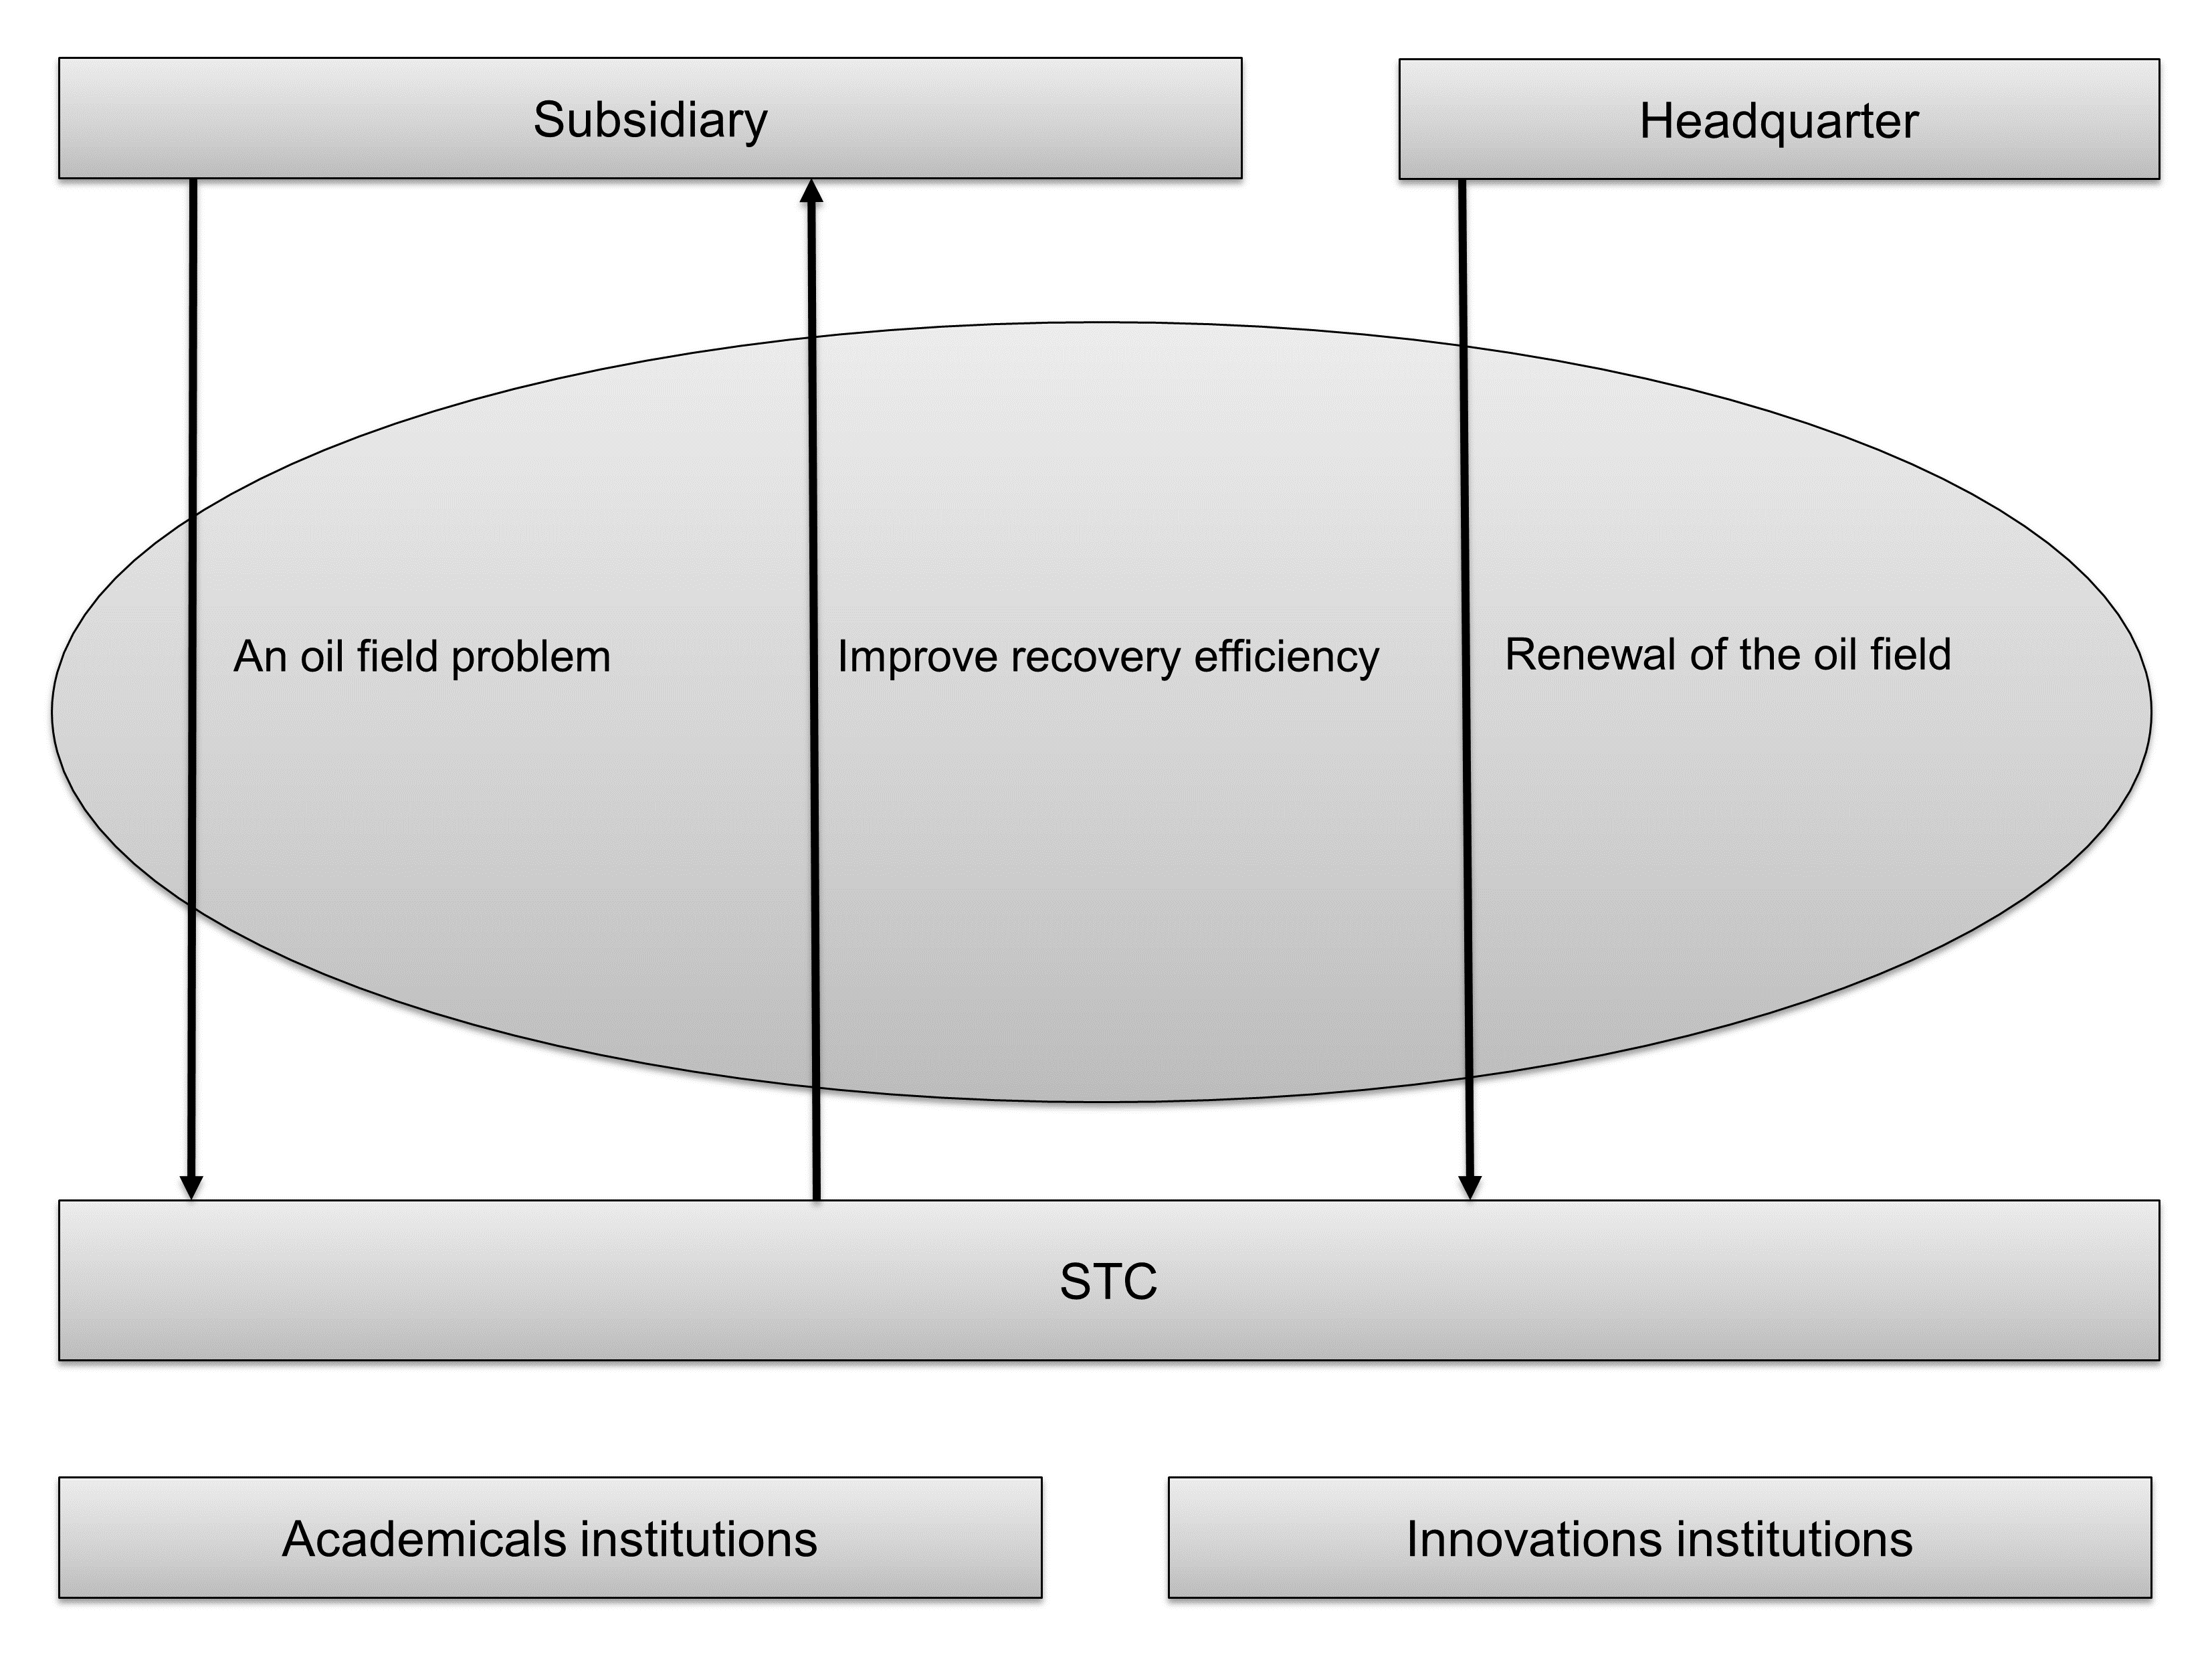
\includegraphics[width=0.8\textwidth]{intro_fig_0_eng}   
	\caption{Industrial value chains.}  
	\label{fig:int0} 
\end{figure}  

In the first model chain, the initiating factor is the problem that arises directly from the development or operation of a particular field.
However, the problem should become a typical one, i.e. typical for several fields, or for one colossal oilfield, and have a significant impact on the oil production process, so that the company's management decides to order the relevant research in any STC, after which intellectual values arise, ready for subsequent use in other fields and other situations.
Another option is the situation when in the course of standard design and service engineering works ordered by the oil company for the development, arrangement, and operation of a particular field.
STC specialists make a predictive forecast based on a posteriori models built on the data and knowledge available to the STC and recommend the Customer to take specific preventive measures and proactively carry out the necessary engineering, geological and technical measures to ensure the further sustainable operation of the field with the high index of recovery.

In the second scheme, the company's management is the initiator of research and development and implementation of the technology.
As a rule, we are talking about the commissioning of sites recognized as unprofitable in the framework of the use of oil production technologies, for example, low-productivity areas with low permeability, fractured reservoirs, low-debit wells, which require, in particular for their development and operation of the intelligent adaptive control of the production process.

In both of the described flow of intellectual values is of the order of the research and development of STC can be built in the purchase of already existing technology on the external market.
However, even in this case, the role of STC is critical regarding technology adaptation, its implementation in a particular field, the collection, and analysis of primary data on the use of technology and the problems arising in this regard.

It is also evident that the transfer of a single technology can be difficult or even impossible due to fundamental differences in the technological structures of the Russian and foreign oil industries.
Therefore, it is necessary first of all to provide a purposeful step-by-step transfer of the optimal technological environment, and for this, it is first of all essential to introduce modern concepts of business processes organization and to follow the main current trends steadily.
Only within the framework of the updated conceptual understanding, the explication of individual technological processes will not remain isolated inclusions, will not dissolve over time, but will serve as the embryos of a new phase, around which the effective crystallization of a new technological structure will begin.
Indeed, the processes of standardization and innovative integrated technological training of personnel play a significant role.
It is possible to direct the inevitable influence of the human factor in the introduction of new innovative technologies in the right direction only by nurturing the project and corporate culture of a new level.

Also, the introduction of almost any modern technology should be accompanied by changes and a presentation of new technologies in its sphere, the information environment of the company, system and application software.
The conceptual priorities here are well known and clearly defined:
\begin{itemize} 
	\tightlist 
	\item Comprehensive digitalization (digitalization) of the oil industry from ``Digital field'' to ``Digital electronic oil company'';
	\item Application of artificial intelligence systems with elements of neural network technologies and machine learning algorithms for process control; 
	\item Wide implementation of Big Data concepts and methods, including cloud technologies, analytical tools, and specialized software.
\end{itemize}

In essence, we are talking about the introduction of Industry 4.0 concept in Upstream.
It is necessary to create conditions for the widespread of digital culture, as well as to ensure a direct interest in the successful digital transformation on the part of employees of all levels and specializations, but above all the top management of the company.
It is necessary to fully involve representatives of the ``digital generation'' in the production process - specialists in Big Data, neural networks, cluster analysis, machine learning methods, as well as existing employees of the company who are loyal to the dynamic digital ecosystem and other employees who can safely work in a vibrant digital ecosystem.
After that, measures can be taken to speed the death of old ``non-digital'' approaches.

As is well known, the smart digital oil and gas field is a system of automatic control of oil and gas production operations, providing continuous optimization of the integrated field model and production management model.
Due to the complexity and fuzziness of geological models (as part of the integrated model) to build a fully automatic control of oil production in the foreseeable period is impossible.
But it is possible to use this standard for the formation of goals for programs to reduce the human factor in the management of the life cycle of deposits.

Intellectual digital field (IDF)- is a class of asset management systems of oil-producing enterprises, built by a formal, integrated asset model, processed by an automated control system that ensures optimal management at all levels of the enterprise while controlling the goals set by the owners of the asset.
The term is based on the concept of intelligent management.
An analog of IDF is the Digital oil field (Digital OilField, DoF), integrated operations management at the area.
A particular concept of this term is ``smart well''.

\begin{itemize}
	\tightlist
	\item formalization of the field information model;
	\item control apparatus; 
	\item the most accurate feedback interfaces (sensors, communication);
	\item interfaces to optimize processes, models and criteria.
\end{itemize}

The necessary conditions for the existence of the intellectual field is:

To ensure the integrity of field management, an integrated asset information model should include and integrate all aspects of existing asset knowledge, including submodels such as:  

\begin{itemize}
	\tightlist
	\item geological model; 
	\item geographic model;
	\item technology model;
	\item logistic model of supply chains;
	\item economic model; 
	\item financial model.
\end{itemize}

The introduction of an intelligent digital oil field is based on open standards ISO 15926, ISA-95, ISA-88.

The intelligent digital field includes several control circuits, first of all:  
\begin{itemize} 
	\tightlist 
	\item The operational loop which provides control over the efficiency of processes for managing field operations (production, monitoring, and control of operating modes and condition of equipment, auxiliary processes, etc.)); 
	\item Modeling circuit that provides a dynamic development management model under varying external (context) and internal (content) conditions.
\end{itemize}  

However, the process of digitalization (digitalization) faces some organizational, administrative and behavioral-psychological obstacles.

\section{Big Data in oil and gas industry}
The importance of taking into account the randomness factor is also confirmed by other promising works on accounting for randomly changing dependencies between permeability and porosity of the formation.
As predictors for the establishment of such dependences for a particular field, in addition to well logging data, it is proposed to use the division into zones with approximately the same conditions of sedimentation.
In the framework of the model used, it is considered that the statistical regularities for porosity and permeability for each of these zones and their parts are the same.

Thus, we see that digitalization (digitalization) is faced in Russian conditions not only with the established administrative-organizational and behavioral aspects of activity in the oil industry but also with physics, the reason for which is the existence of random fields.
This means that the physics and models of geophysical environments, although they cannot be entirely attributed to the digital stage and the Big Data era, still have a chance of survival in the transition to Industry 4.0.
Together with physics have a chance of survival, at least at the initial stage, and the Russian STC in the oil industry

For this reason, the analysis of the activities of Russian STC in the oil industry is still of great interest, including in the context of innovative and technological solutions developed by these STC.
To be entirely carried out, such an analysis requires the development of integrated criteria for the effectiveness of the STC.

The Big Data approach is characterized by exponential growth in the number of measurement operations and their corresponding data.
At the same time, both the data itself and the algorithms for processing them, implemented in the form of information and analytical computer systems using network and cloud technologies, along with human resources, technological know-how, and capital, become one of the main assets of industrial, including oil companies.
Data Mining analytical tools are at the same time the essential tools to achieve a competitive advantage in the market.
Systems for the collection, primary processing, storage and security of information are also necessary.
It is not surprising that many experts and analysts say now: ``we have realized that there are terabytes of information around us, and now we need to understand what to do with these terabytes''.

It is possible that the exit is a departure from traditional computer architectures in the direction of neuromorphic computational and analytical systems equipped with deep machine learning algorithms.

It is also necessary to use the methods of probabilistic programming based on the Bayesian inference since often a large proportion of sensors that monitor the digital field, characterized by a situation where the random spread of the observed values of the measured values is comparable to the price of the division of the measuring instrument.
The reason for this is an attempt to control complex technological processes by controlling an increasing number of degrees of freedom of complex distributed systems.
A corresponding increase in the number of signals from measuring devices with the simultaneous requirement to increase the accuracy of measurements leads to a decrease in the useful signal/noise ratio for a large proportion of measured values and parameters.
There are cases when a further increase in the accuracy of measurement of a particular technological value (parameter) is impossible due to the achievement of the physical and technical limit for this method of analysis or too costly.
At the same time, increasing the useful signal/noise ratio for this type of measurements carried out in real conditions is also either technologically impossible or very costly.
As a result, an increase in the total number of measured parameters of the system or process does not lead, starting with a specific limit value, to an improvement in the accuracy of monitoring data and the quality of control and management.
The output is seen in the development and use of hierarchical adaptive controllers based on fuzzy logic, as well as neural network systems, including algorithms for deep multi-layer learning with elements of formation of abstract clusters of data within the neural network (deep learning technology and neuromorphic computing).
A neuromorphic computer network, equipped with a specialized algorithm of configuration and training, is able in the long term to absorb the flow of Big Data generated by sensors and sensors of the digital field and subject this flow to multi-criteria analysis, separating essential data from non-essential.
In the same vein, it should be considered, and the prospects for the machine to machine communication, when armed with neural processors of the device along the oil transportation line from the well to pumps share data with the purpose of optimization of technological modes and predictive forecasting of adverse, unplanned and potentially dangerous situations.
This approach is entirely consistent with the concepts of \textit{Internet of things} and \textit{Industry 4.0}.

Another approach to the utilization of Big Data generated by a digital (digitalized) field is to apply a universal code based on the Shannon information entropy theory and the Laplace and Krichevsky predictors to the archiving data flow based on the identified comprehensive system for this flow.

This kind of ideas refers us to the works of the late Soviet period (late 70's-early 80's of the last century) in the field of automation of the oil and gas industry.
Then, for example, the approaches of constant diagnostics of drilling equipment or deep sucker rod pumps based on continuous wattmeter were proposed, as well as algorithms for energy-efficient control of facilities due to adaptive speed control of electric drives of various types of equipment.
Of course, in modern oil production and drilling equipment, many of these principles have already been implemented in different versions.
Thus, to ensure high-precision drilling of horizontal shafts with multi-stage hydraulic fracturing, Gazprom Neft has created a center for geological support of drilling, whose specialists manage drilling in on-line mode under remote access using rotor-controlled systems.
In particular, similarly, the latest digital technology is found and combined in a real field with electro-mechanistic technology.

We cannot ignore supercomputer computing technologies and their application in the oil and gas industry.
Over the past 20 years and to the present time, foreign countries, together with oil and service companies, have made significant efforts to stimulate research and applied for work on the long-term development and effective implementation of high-performance information and computing technologies to solve computational problems in the search, exploration, and development of hydrocarbon deposits.
As a result of this activity, foreign oil and service companies gained competitive advantages and were able to oust Russian companies in the market of oilfield services significantly. Including the production, sale and maintenance of software, production and use of supercomputers (high-performance computing systems), which led to the technological dependence of Russian organizations, a high level of maintenance costs, lagging in scientific and technical development, the growth of the threat to information security and, ultimately, the risk of complete loss of a promising high-tech market of production, sale and maintenance of complex scientific and technical products and information and computing services.

At the same time, in Russia, in the last 20 years, the development and production of domestic software and hardware systems and software aimed at solving the problems of prospecting, exploration, and development of deposits have significantly decreased.
The lag in the development of scientific research, the creation of software products, the quality of training of specialists from the level achieved by foreign countries was manifested.
In some areas, there is an almost complete replacement of domestic equipment and technologies with imported products.
In the domestic market, more than 80\% of high-level computer technology for solving geological and geophysical problems is imported.
When using external information and computing technologies in the field of Geophysics and Geology, there are inevitably prerequisites for the leakage of valuable information about the national subsoil and strategically essential resources.
Such a situation, under certain foreign policy circumstances, can have a very detrimental effect on Russia's energy security.
This situation does not mean that the state should limit access to the domestic market of high-performance computing technologies in this area from abroad using organizational or economic levers.
Instead, it is necessary to stimulate and initiate the creation and implementation of high-quality domestic software products that can effectively compete with similar foreign developments.

There are quite good economic reasons for this.
For example, standard software packages of leading foreign companies (Petrel, Eclipse, Roxar) used for seismic and geological-hydrodynamic modeling cost about 4.5 million rubles for one workplace plus  1 million rubles annually is paid for support.
At the same time, in many software packages, there is a limit on the use of the number of nodes of the cluster computing system.
For the possibility of using each next computational node, you have to pay about 12 thousand dollars.
Thus, for an oil and gas company of average size, which involves about 100 geological jobs of about 200 potential users in geophysical works, and half less for hydrodynamic modeling, if necessary, the full use of the computational cluster of 400 nodes, the initial cost of costs is not less than 1350 million rubles plus the cost of annual support (expert evaluation).
At the same time, the domestic software package \textit{tNavigator} for the calculation of hydrodynamic models of production of the company ``Rock Flow Dynamics'' is supplied without limitation on the number of involved computing nodes, are several times cheaper and considers several times faster.

The tasks of development of scientific research, creation, and implementation of the most useful information technologies and the obstacles that stand in this way were noted in the Energy strategy of Russia until 2030.
Awareness of the importance of the development of supercomputer technologies and algorithms and software for high-performance computing for modernization and innovative development of various sectors of the economy is recognized in Russia at the state level.
This position reflected in the decisions of the Commission under the President of the Russian Federation on modernization and technological development, decisions of the Security Council, reflected In the strategy of development of the geological industry until 2030 and the Energy strategy of Russia until 2030, the State program ``Information society for 2011 -- 2020'', the Project ``Creation of a system of training of highly qualified personnel in the field of supercomputer technologies and specialized software'' Of the Commission of the President of the Russian Federation on modernization and technological development of the Russian economy, speeches of specialists, developers of supercomputers, software for the oil and gas industry, representatives of oil and gas and service companies concentrated in the solution of the First conference ``Supercomputers in the oil and gas industry''.

\section{Criteria for assessing the scientific effectiveness of the STC}

Let us turn to the criteria for assessing the effectiveness of the STC in the oil and gas sector of the Russian Federation.
The definition and practical use of such criteria are one of the objectives of this work. 
First of all, let us consider what types of STC are represented in Russia for activities in the oil and gas sector.
They can be divided into the following groups:

\begin{itemize} 
	\tightlist
	\item scientific and technical centers for large Russian oil and gas companies such as Gazprom, Rosneft, LUKOIL, TNK-BP, Gazprom Neft, Surgutneftegas; 
	\item state scientific and technical centers; 
	\item independent Russian scientific and technical centers; 
	\item Russian scientific and technical units of foreign service companies, for example, DCS Department in Schlumberger.
\end{itemize}  

Let's consider the activities of STC in the oil and gas industry by short-term and long-term perspectives. 
Both of these aspects have both economic and technological components. 
Let us first consider the short-term aspect.
As previously noted, the economic component in assessing the efficiency of STC activities in the short term is determined by the dynamics of the company's profit from the sale of oil, gas and their products.
At the same time, from the STC as a commercial organization, its internal structure should be optimized for the effective execution of orders, and the experience baggage and competencies should meet the current needs of the market.
PR-technologies also play an essential role here.

Indeed, the analysis of the issues of the journal ``Oil and Gas industry'', conducted with the participation of the author of this work, shows that in recent years in the articles appeared a large number of ``digital'' terms (topics) such common memes as ``data'', ``method'', ``system'', ``study'', ``sensor'', ``standard'', ``scheme'', in contrast to those present in the earlier issues  ``pipeline'', ``pipe'', ``specialist'', ``Geology'', ``field'', ``technology'', ``territory'', ``well'', ``refinery''.
Is it true that in the Russian oil and gas industry is growing interest in the use of information technology and the use of intelligent data analysis methods are becoming increasingly popular in the oil sector of the economy?

Undoubtedly, however, the articles in a trade magazine, Pestryaev such buzzwords also reflect a splash.
Whether this wave will turn into a long-term technological trend will show the development of the situation in time.
Thus, the economic situation determines the current advertising campaign in the activities of the STC, implemented through publications in open editions.
Of course, not all publications in industry scientific journals are speculative and market-advertising.

Let us consider the assessment of the STC's activities from the long-term perspective.
The economic component here can be characterized by using standard integrated indicators of economic analysis of the enterprise, such as integrated financial indicators for the operating period of activity or specific financial indicators per employee.
The results of a study \footnote{\url{https://www2.deloitte.com/content/dam/Deloitte/ru/Documents/energy-resources/Russian/key-trends-of-market-research-in-oilgas-industry-in-russia.pdf}}
by Deloitte, which evaluated the activities of 33 STC operating in the oil sector of the Russian economy, including all of the above types, are shown in Figure.\ref{fig:int1}.

\begin{figure}[ht]
	\centering     
	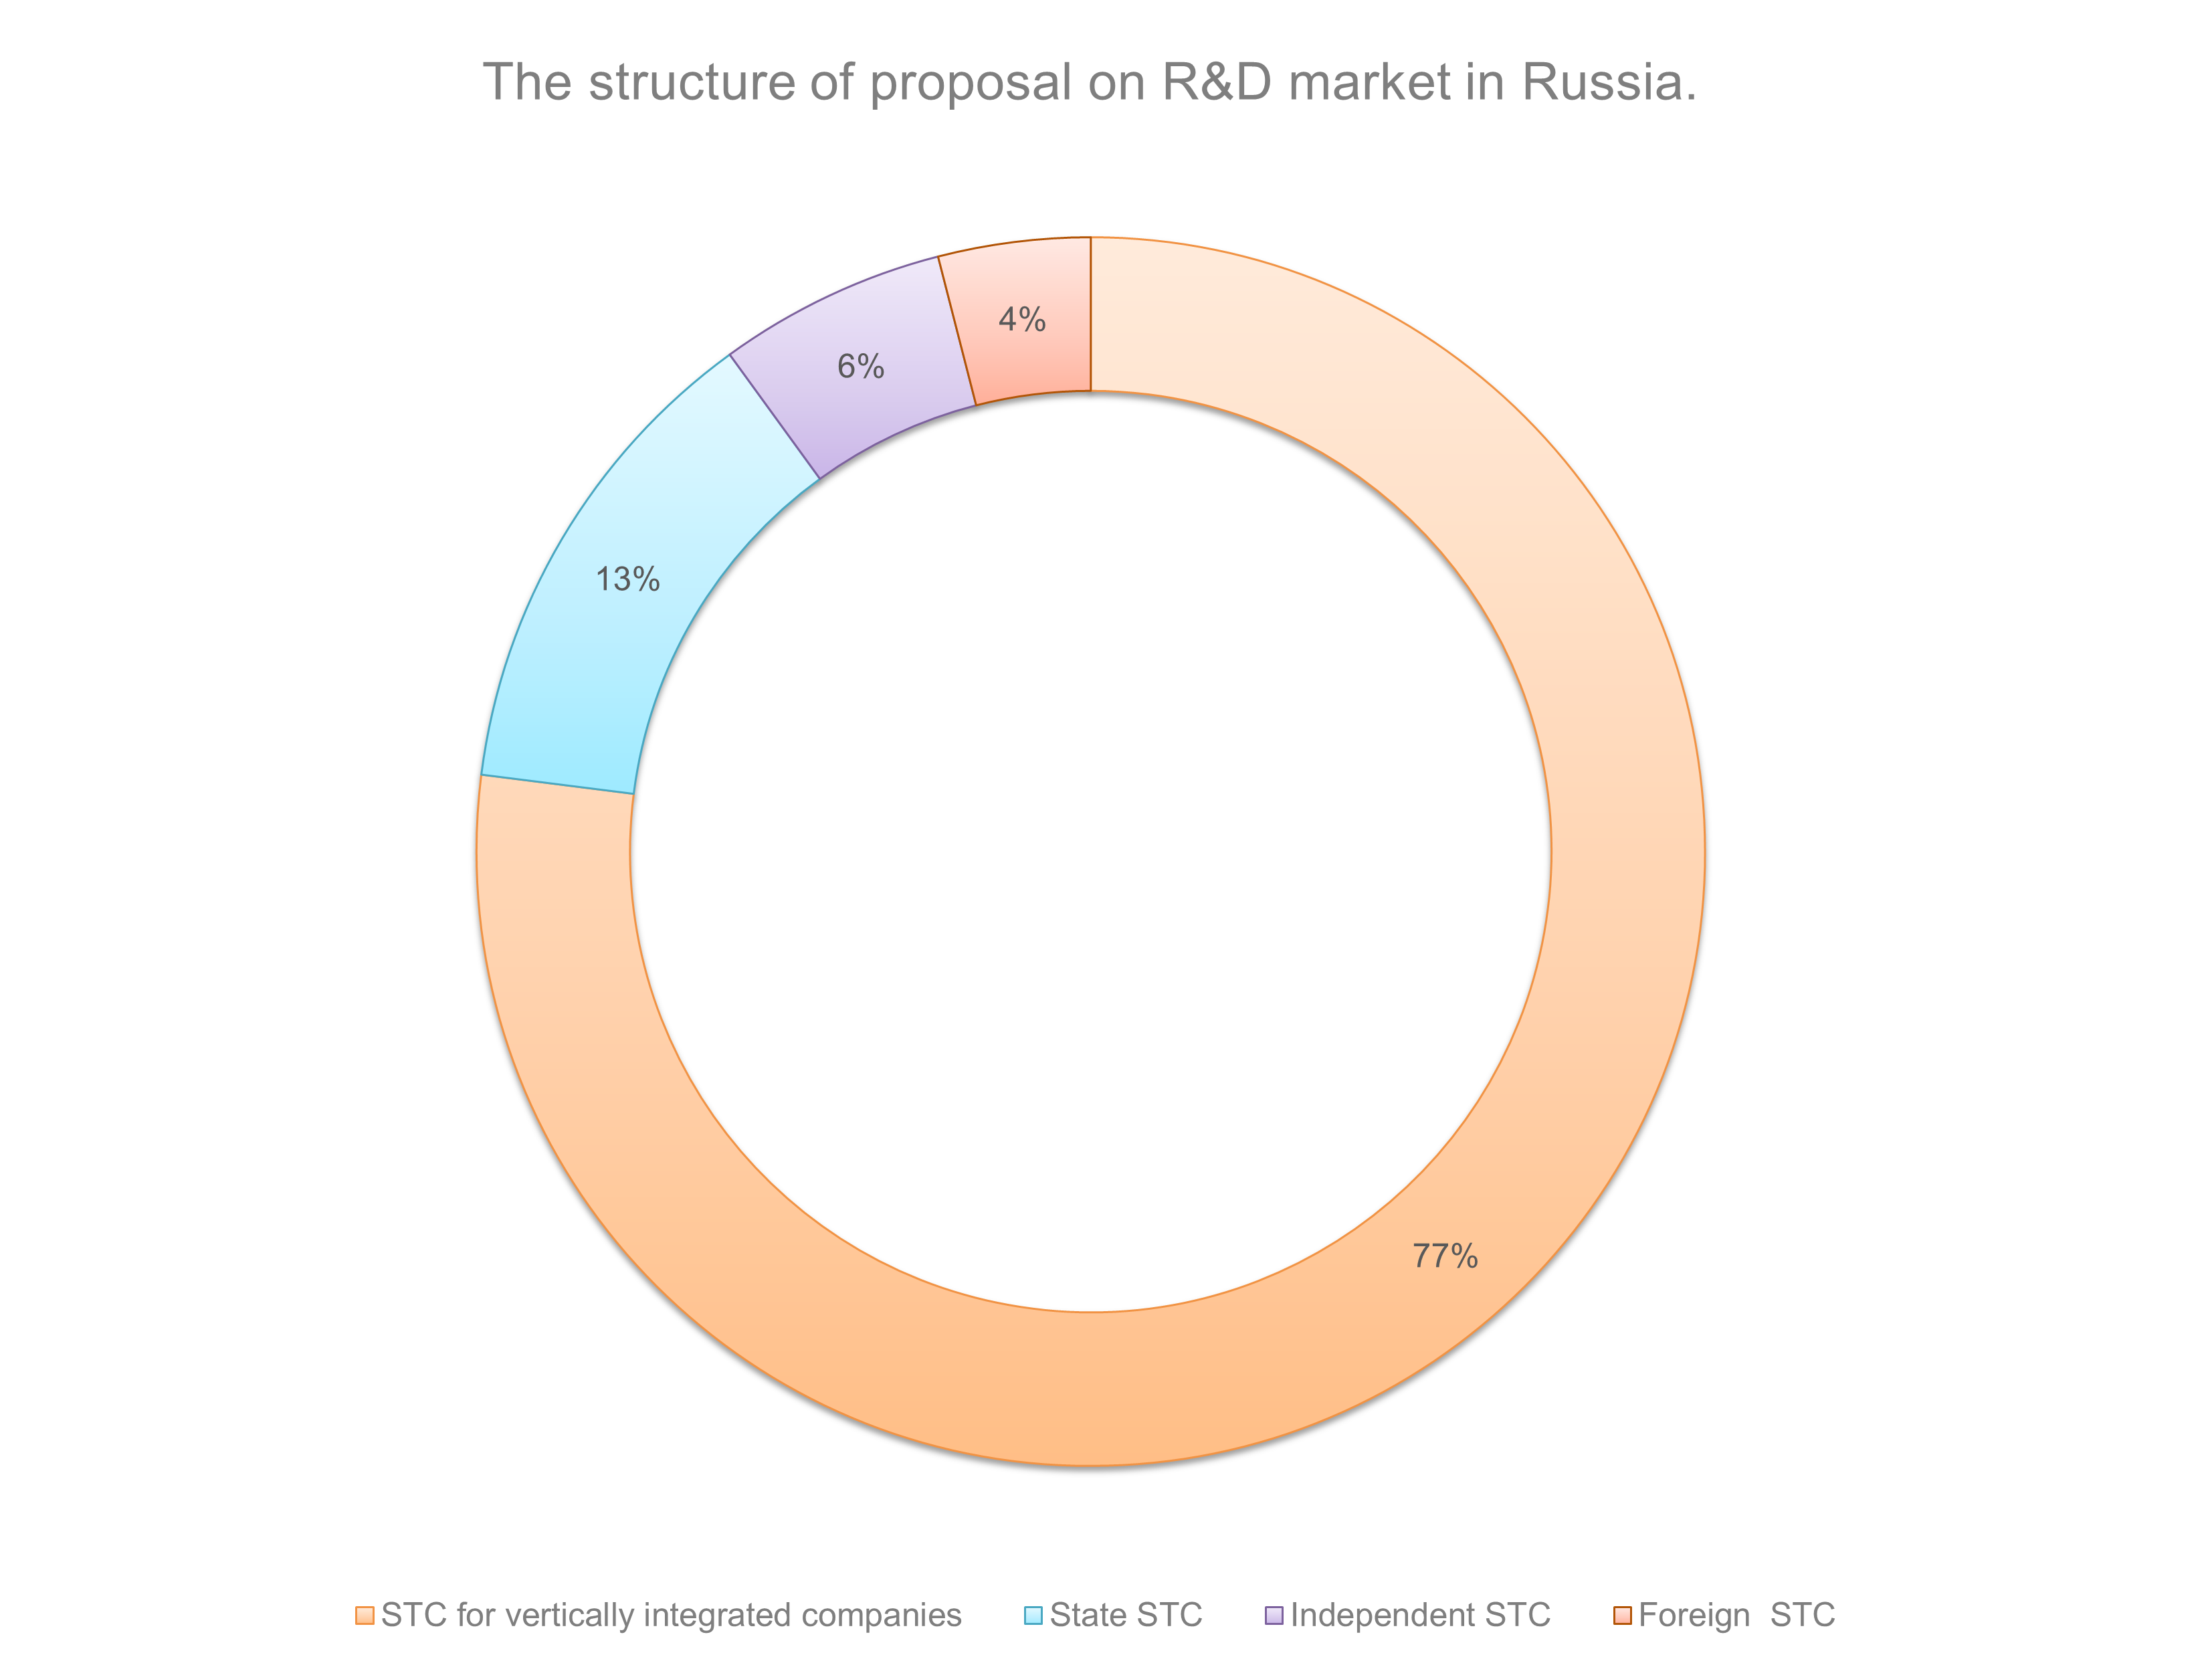
\includegraphics[width=0.8\textwidth]{intro_fig_1_eng}   
	\caption{The structure of supply in the market of research works in 2009.}  
	\label{fig:int1} 
\end{figure} 

So, we see that despite a specific actual orientation of the industry to import technologies, the share of STC of foreign oil service companies is low, while the percentage of STC in large Russian vertically integrated oil and gas companies exceeds the total part for STC of all other types.
Such deviations do not mean that the industry uses domestic technologies, but only that significant industry players prefer to develop and adapt imported techniques on their own.

Given the current structure of the technology development market in the oil and gas sector of Russia, close attention should be paid to the activities of independent STC, taking into account the time of their operation in the market.
So it is possible to reveal the hidden technological trends and actual production and technological requests in the oil industry of Russia.
Of course, if the STC is young enough, for example, operates in the market for no more than 5 years, this does not mean that such a company can not demonstrate high efficiency, but it is still evident that the activities of quite young companies in the market require additional analysis in terms of assessing the effectiveness and identifying promising trends.

%\begin{figure}[ht]
%	\centering     
%	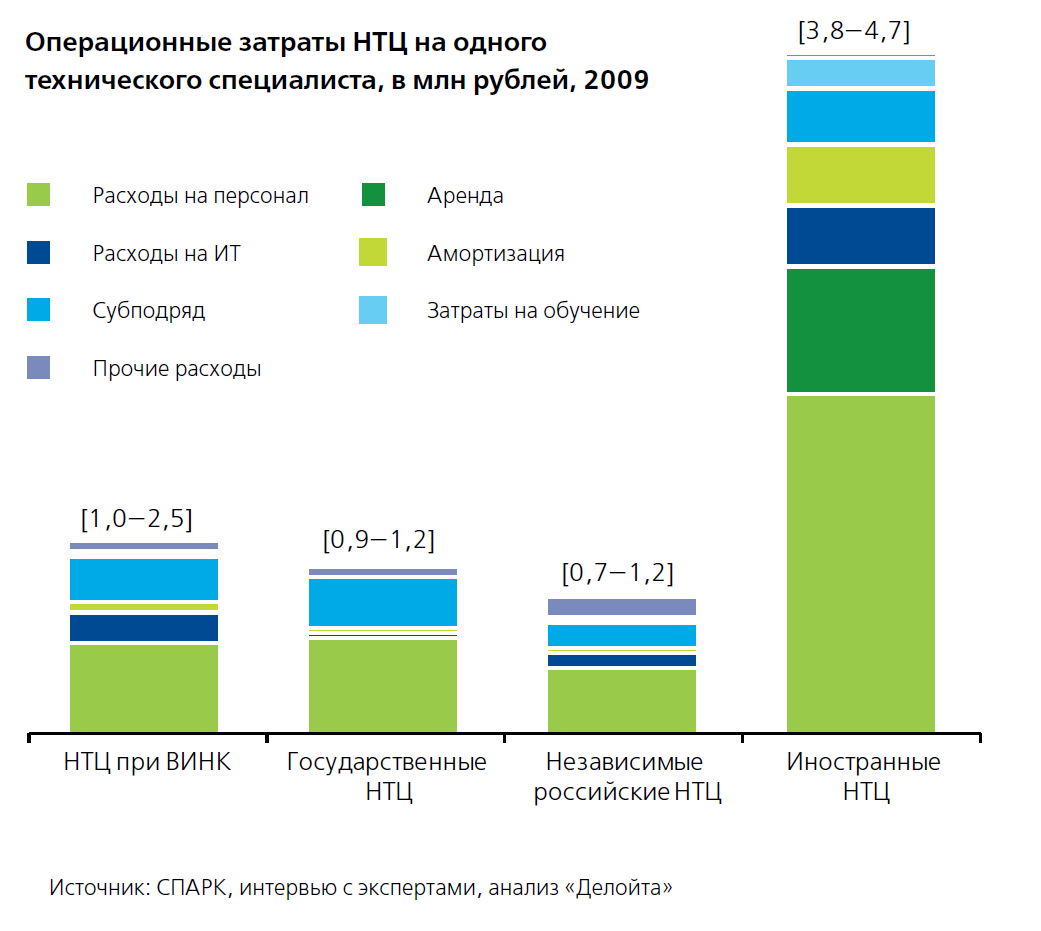
\includegraphics[width=0.8\textwidth]{int2}   
%	\caption{Operating expenses of STC on to one technician 2009 (mln. roubles)}
%	\label{fig:int2} 
%\end{figure} 

Let us turn to the description of the criteria for the effectiveness of the activity of the Scientific and Technical Center in the long term, related to the actual production of the Scientific and Technological Center in the form of new technologies.
To do this, we consider an approach based on the analysis of digital artifacts of STC activities, primarily various types of documents in electronic format, reflecting the results of STC activities and available for review from open sources.
These types of digital artifacts can include:

\begin{itemize} 
	\tightlist 
	\item industrial e-libraries documents; 
	\item patents; 
	\item scientific papers in industrial journals; 
	\item open access documents about oil and gas industry. 
\end{itemize}  

All of these documents may be subjected to computer analysis, primarily a highly promising method of the topic model, the essence of which is the use of bi-clustering, that is, simultaneous clustering of words and documents on their semantic proximity.
In this case, as a rule, Dirichlet's hidden placement is used, which, although convenient for algorithmic computer calculations when conducting thematic modeling, is not entirely justified from a linguistic point of view.

The results of the topic modeling conducted by the author of this work for the articles in all issues of the journal  ``Oil and Gas industry'' for the period from 2008 to 2016 (which was mentioned in this Chapter earlier) showed that contrary to the initial assumption about the smooth evolution of the topics identified in the framework of thematic modeling from issue to issue, in various volumes of the journal were fixed fundamentally different subjects.
Does this mean that the journal focuses on the latest technological developments in each new issue and does not refer to outdated and unused technical approaches? Yes and no.
The tactical component in the selection of publications by the Editorial Board to increase the attractiveness of the magazine in a wide range of oil and gas and related fields is visible.
This tactic is the essence of specialized publishing.
At the same time, the fate of the technologies mentioned once cannot be judged by such single publications.
Have they been rejected in practice, or have they been tried and proven to be untenable? 
Or, perhaps, have you become a part of the oil industry's tools during the analyzed period of 8 years? 
Such conclusions cannot be drawn from the information analyzed.
What is the way out of this situation?

It consists in the analysis of a broader range of documents, from patents to abstracts at industry conferences.
These documents can be subjected to cluster analysis using different algorithms.
At the same time, if we are talking about using a classification with a training template (``with a teacher''), then expert descriptions of the most modern technological trends and innovative topics in the oil and gas industry can be chosen as a training template.
The same sets of analyzed documents that will not be included in the classes (clusters) defined in this way should not be considered a priori as `noise", but should be subjected to additional analysis for the fact that they represent evidence (digital artifacts) of latent innovation and technological trends.

On the basis of this performed clustering (classification) of documents (digital artifacts of innovation and technological development of the oil and gas industry) can be defined multicriteria integral numerical performance indicators of specific STC, calculated on the basis of the distribution shares of digital artifacts produced by employees of the STC, clusters (classes).
Changes in such distributions over time can serve as a basis for posterior predictive modeling of the performance of specific STC in future periods of time.

A separate topic, although related to the technical side of this study, is the provision of information exchange, access to documents (digital artifacts) and their pre-processing, including uniform electronic formats and stemming.

All these issues will be discussed in the following chapters of this work.

\chapter{Related works}
\section{Organizational efficiency}

Scientific management guru Michael Porter in his book ``Competitive advantage of nations: creating and sustaining superior performance'' \autocite{porter2011competitive} highlights the effectiveness of research work as one of the processes of competition between countries. 

There are many approaches to the interpretation of the concept of performance in general and in research, in particular. 
But it is essential to understand that efficiency is not a number \autocite{quinn1983spatial, wolfe1994organizational, daft2010organization}.

The main components of the research process include the formation of researchers collaboration, the process of creating a scientific article and its publication. 
The published scientific article is one of the embodiments of the results of scientific research. 
There are many methods of conducting research. 
Most of them use the structuring of research activities into stages to simplify its understanding. 
For example, in the book \cite{lipch2013met} the following seven steps are highlighted:

\begin{enumerate}
	\tightlist
	\item Selection of the research topic;
	\item Study of world experience on the chosen topic through scientific sources;
	\item Preparation of research work plan;
	\item accumulation of material to test the validity of the proposed hypothesis;
	\item Data processing, model building;
	\item Analysis of research results and conclusions;
	\item Documentation of research work.
\end{enumerate}

Thus, the creation of a scientific article, as a result of scientific research, can be presented in the form of a formalized process implemented by the participants of the research group. 
This process belongs to the category of everyday social interaction. 
And its study is one of our tasks in this research. 
Therefore, the author set the task of considering the process of joint research activities and writing a scientific article with subsequent publication. 
Also, the author of this study tried to take into account the processes of collective thinking and communication, noted in \cite{mkrt1995f}.

In scientific practice, researchers should share the results of their research with colleagues. 
Publication of an article in a scientific journal is a form of communication between a researcher and the scientific community \cite{danil2016o}. 
In addition to the publication of the article, communication can be carried out in the form of publication of monographs, abstracts of conferences or patents, as well as personal presentations at conferences and seminars. 
Therefore, scientific research cannot be considered in the in isolation from the publication process.
Thus, the Editorial Board of scientific journals and committees of scientific conferences should be included in the broad collaboration of the research team.

In the simplified view of the Editorial Board and the committees of the conferences are grouped not by formal categories like  Code of State Categories Scientific and Technical Information 
%\footnote{\url{https://ru.wikipedia.org/wiki/Государственный_рубрикатор_научно-технической_информации}} 
but in specific mental codes \cite{gary2016unpacking}, hidden behind the descriptions of the format and editorial policies.
An example of such mental code would be ``we only accept articles from members of the SPE (Society of Petroleum Engineers)'' or ``Authors must have a degree in CS''.
The concept of mental code is widely used in the analysis of grouping \cite{sidor2006g, gentner2014mental}. 
The mental code can be made up of individual fragments, like a DNA molecule. 
It is essential to understand that a new member is accepted into the community by the coincidence of the mental codes. 
That, in our case, means acceptance by the Editorial Board or Committee of the conference of scientific work for publication.
Sometimes a part of the mental code can be declared.
But this does not mean that a significant portion of it, by which the decision will be made, does not remain the internal property of the Editorial Board or the Program Committee.
In this case, the author will be puzzled by the fact that he was ``unmotivated'' refused, as a significant part of the mental code of the Editorial Board or the Program Committee of the conference is not available to him.

The process of publication of a scientific article also has formal stages, which, however, does not reflect the network process of work on the result:
\begin{enumerate}
	\tightlist
	\item Announcement of the date and topic of the conference;
	\item Call for papers;
	\item Peer review;
	\item Creating of bilingual text of the paper;
	\item Creating of a presentation;
	\item Oral performance of the presentation;
	\item Preparing text for publication;
\end{enumerate}

Thus, it is possible to speculate about the fundamental process contains the logic of the extension of the small co-author's group to broader groups.
Broader co-authors groups include the representatives of the Editorial Boards, committees of conferences, guest authors, translators, experts, presentation designers.
The consideration of such collaborations is necessary to understand the process of publishing scientific articles and then estimate the contributions of individual participants.

The division of labor \cite{taylor1914scientific} characterizes the maturity of production processes. 
For the scientific writing process, it means mean that specialized pools of resources are created to maintain certain stages without personification. 
For example, from the Soviet Union past, we know the slang term ``cooperative for recording formulas'' concerning Ph.D. theses. 
Despite the marginality of this phenomenon, which was publicly condemned and flourished due to the demand in a narrow specialization, the author sees in it the first prerequisites for the division of labor in the production of scientific research and publication on its basis. 
Currently, due to the acceleration of research production, new forms of division of labor (and new requirements for the effectiveness of research personnel) have appeared, which need to be studied.

The question of collective knowledge creation and writing research, in particular, has many aspects related to the ethics of the researcher. 
Should the author fully comply with all stages of work on the study? 
If there are two co-authors in work, then what division of labor does not violate the ethical norms of the researcher? 
What roles are ethical among co-authors? 
In the well-known ``Course of Theoretical Physics'' by Landau and Lifshitz \cite{landau2013course}, what role did L.D.Landau play, and which E.M.Lifshitz?

After the unification by the mental code, the development of relations within the framework of collaborations takes place in a full (with external participants) and narrow (within the research group) sense.
Strengthening co-authorships as a result of writing several papers creates more sustainable working groups. 
There are examples of ongoing co-authorship over decades.
On the other hand, there are examples when, having written a single research paper, the authors no longer collaborate.
What are the reasons for sustainable associations in co-authors?

The author believes that many scientific and methodological sources focus on the technology of writing a scientific article and its design, but not studying the process of creating scientific articles. 
Therefore they consider this work practically useful for administering and planning research regarding scientific management according to F. Taylor \cite {taylor1914scientific}.

The problem of an objective assessment of the effectiveness of R\&D has been in the center of attention of researchers for a long time, and this, first of all, is related to the issues of financing both budget and within grants.
In the framework of the traditional approach, the following indicators for evaluating the effectiveness are highlighted \cite{korol2014krit}:

\begin{itemize}
	\tightlist
	\item Financial
	\item Human resources
	\item Innovational
	\item Bibliometrical
\end{itemize}

Actually, within the bibliometrics, the following parameters are taken into account:

\begin{itemize}
	\tightlist
	\item The number of publications in international journals characterizes the quality of articles;
	\item Citation indicator and Hirsch index show the degree of significance of the research and recognition of scientific schools by the world community;
	\item ``publication load'' of scientists shows the productivity of scientists;
	\item availability of patents;
	\item co-authorship with foreign scientists is an indicator of international cooperation.
\end{itemize}

As many researchers have noted \cite{vonortas1995new, veugelers1998collaboration, faems2005interorganizational}, this set of parameters is far from perfect, because it does not provide a completely objective picture of the research of the selected scientist or team.
For example, the Hirsch index depends on the discipline, and it also does not fall if a person has not published new works for ten years or more. 
The citation bases WoS and Scopus, firstly, reflect inadequately research in Russian, and secondly, unequal shares are assigned to different disciplines.
This study tests the hypothesis that improving the quality of the evaluation of the effectiveness of research and development is possible through the consideration of additional factors, which will be discussed later.

Organization effectiveness is a very complex and multifaceted concept.
It is influenced by various factors.
One of the most important precursors of the market success of a research and development company is a well-developed communication and cooperation between employees.

Many theoretical and practical studies demonstrate the relationship between the productivity of an organization and the communication structure of its employees, for example, see \cite{allen1984managing,noe2006human}.
The study of the social structure of organizations and professional communities is becoming one of the main areas of applied analysis of social networks.
In the field of public relations and management, communication patterns within organizations are studied in depth.
This research began in 1956 with the work of C.H.Cooley ``Social Organization'' \cite{cooley1956social}.

Information about employee interactions can be obtained in various ways, for example, through corporate databases, public surveys, and personal reports.
However, the data obtained in such ways must be interpreted with some reservations, since they do not reflect the whole mechanism of professional interaction in integrity.
According to Wasserman and Faust \cite{wasserman1994social}, about half of what people report about their interactions is wrong for one reason or another.
Thus, people are not very good at communicating well with their relationships, so ways to collect data should avoid such subjectivity.

The source of such information may be Google Scholar, arXiv and other online libraries.
Consideration of open scientific communities is as impressive as the narrowing of the sample to one country, industry, and organization.

One of the more objective ways of analyzing human interactions is a formal conceptual analysis (FCA).
Formal concept analysis (FCA) is a way to analyze a collection of objects and their properties. 

A {\em formal context} is a triple $K = (G, M, I)$, where $G$ is a set of objects, $M$ is a set of attributes, and $I \subset G \times M$ is a binary relation that expresses which objects have which attributes.

In FCA implication $A \to B$ for subsets $A$, $B$ of the set of attributes $M$ $(A,B \subseteq M )$ holds if $A' \subseteq B'$, i.e. every object possessing each attribute from $A$ also has each attribute from $B$.

An {\em  association rule} is an implication expression of the form $X \to Y$ , where $X$ and $Y$ are disjoint sets, i.~e. $X\cap Y = \emptyset$. The strength of an association rule can be measured in terms of its {\em support} and {\em confidence}. Support determines how often a rule is applicable to a given data set, while confidence determines how frequently items in $Y$ appear in transactions that contain $X$. See \cite{ganter2005formal} for a detailed introduction to the subject. 

In this paper we utilize the FCA framework for studying the author - keyword relationship. For us
\begin{itemize}
	\item $G$ denotes the set of keywords.
	\item $M$ stands for the set of all co-authors of the papers.
	\item $I \subset G \times M$ is a binary relation. One has $(g,m)\in I$ if $m$ co-authors a paper for which $g$ is among the keywords.
\end{itemize}

Then the association rules are interpreted as indicators of connectivity between different research fields, and also used to recognize weak ties between authors of different papers.

The idea to apply FCA in the context of social network analysis is not new. In \cite{kurtz2009collective} it was used for collective network analysis.
In \cite{snasel2009analyzing} a combination of Formal Concept Analysis and well-known matrix factorization methods were used to address computational complexity of social networks analysis and the clarity of their visualization. 
Bi-clustering and tri-clustering were used in \cite{gnatyshak2012gaining} to analyze data collected from the Russian online social network Vkontakte for extracting groups of users with similar interests, finding communities of users which belong to similar groups, and revealing users’ interests.
FCA was extensively used for analyzing social networks based on co-references, see \cite{kuznetsov2007reducing},
and detecting criminal networks \cite{poelmans2012semi}.
For other applications of FCA in social network analysis see \cite{poelmans2013formal}.
Another rather detailed overview of FCA-based applications for
Social Networks Analysis could be found in \cite{pensa2005towards,obiedkov2007social,aufaure2013advances}.


One of the particular cases of communication is cooperation, which can in the case of research work go in collaboration with the creation of scientific publications.

The publication of scientific research is the primary object by which the effectiveness of research work is assessed.
Therefore, it is essential to follow the process of this process, starting with the birth of the research idea, conducting the experiment and ending with the publication of the work.
It is necessary to analyze what conditions contribute to the successful publication of the article.
As part of this study, the ratio of publications of individual scientists and research teams was studied. 
It has been shown that over the past decade there is a clearly expressed tendency of scientists to unite in groups of co-authors to publish articles.
From this, we can conclude that one of the factors that positively affect the publication of works is the unification of people into teams.

In turn, team building is also victorious and unsuccessful, it is also amenable to study, as a result of which it is possible to single out the conditions for successful team building.
The task of finding the optimal parameters of the team of co-authors for the most productive writer of scientific articles belongs to the class of optimization problems.
Traditionally, researchers pay attention to the following parameters that are important for productive scientific creativity:

\begin{itemize}
	\tightlist
	\item Team size         
	\item Community mental codes
	\item Emploee competences
	\item Week connection
\end{itemize}

Unlike the size of the team, which is a visible, not a hidden sign, and also easily formalized, the sign of the mental models of the community is much more difficult to identify and fix.
Many researchers have noted the importance of changes over time in mental models in addition to the structure of the team \cite{klimoski1994team, morgeson1999structure}.

The concept of a mental model is the development of the concepts of \cite{walsh1995managerial}, knowledge structure \cite{fiske2013social}, knowledge schemes \cite{sims1986thinking}, and the implicit theory \cite{brief1983cognitive}.

The author of this study interprets the concept of the mental model as a strategic consistency of team competencies.
For example, the mental model of ``Agile geoscience'' \cite{hall2011shale} of the largest community of geophysicists is based on the competencies of ``flexible techniques'' and ``geology''.

Researchers agree that the coincidence of the mental models of team members has a positive effect on the performance of \cite{lim2006team, mathieu2000influence}.
This fact addresses the connection between the mental model of the team and the full team code, which is described in more detail below.

The formation of the primary system of internal interaction within the team according to the study \cite{harper1985power} occurs when the participants meet the principle of complementarity.
Nevertheless, one cannot completely deny the value of homophilic competencies.
In many works, the dynamic structure of hemophilia is noted \cite{mcpherson2001birds, snijders2010introduction, steglich20108}, during which two processes take place in parallel.
On the one hand, individuals similar to each other form social ties (social selection).
On the other hand, people already connected adopt the behavior of each other (social influence).
The combination of these factors results in a homogeneous social system, in which between individuals with similar behavior and characteristics there is a connection, while the nature of the relationship can be both formal and informal.

Although connections between individuals with similar characteristics are more likely than those between unique ones, the level of similarity is also essential.
In the \cite{block2014multidimensional}, it was shown that cultural similarity in more than one indicator leads to the fact that people are less likely to form relationships with each other.
The author explains this effect by the fact that people who are too similar in many respects, as a rule, cannot bring something new and constructive into mutual relations or a team.
Productive cooperation requires not only the similarity of interests is necessary, but also a variety of professional and life experience that allows us to offer multi-dimensional approaches to its solution.

\section{Scientific text}

Text analysis is sometimes called \textit{Text mining}. 
The essence of this process is the transformation of data (text) into high-quality information capable of bringing knowledge.
The critical point is that in obtaining knowledge of human costs should be minimal.

The knowledge obtained from the text becomes the basis for making management decisions in the organizational environment.
A separate process is considered the receipt of text, sometimes called the creation of the body of texts.

The real world is reflected in the texts with the help of the authors, and the process of analyzing the text does the opposite: from the texts, it compiles information about the real nature of things.

The multimode approach to text analysis is the process of taking into account the information accompanying the main text.
For example, the address of a letter, the number of a newspaper issue with news, or the names of the co-authors of a scientific article.

Formally, text analysis is performed in the following sequence:
\begin{enumerate}
	\tightlist
	\item text language analysis;
	\item text content analysis;
	\item getting information about the author of the text;
	\item deduction of certain variables characterizing the nature of things in the text.
\end{enumerate}

Let us consider in more detail the methods of working with texts of scientific articles.

\subsection{Text preprocessing}
Text processing tasks were arranged in the 60-70 years of the 20th century in the processing of natural language \cite{weizenbaum1966eliza, kuvcera1967computational}.
It was necessary to bring the text to a more convenient form for further analysis.
This procedure is commonly called \textit{text normalization}.
For the normalization of text using regular expressions, the concept of which was developed by S. C. Wedge \cite{kleene1951representation}. 
One of the first people who used regular expressions in the test was K. Thompson \cite{thompson1968programming}.

At present, the task of normalizing the text has expanded considerably.
It is necessary not only to highlight words but also to take into account special symbols denoting emotions (Emoji), such as 8-)\cite{eisner2016emoji2vec}, highlight hashtags \cite{o2010tweets}, highlight hyperlinks \cite{bingel2017identifying} and process citations \cite{jha2017nlp}.

The task of lexical analysis is to divide the text into parts: sentences, words, letters.  
Sometimes lexical analysis is called tokenization from the English word \textit{tokenizing} \cite{lovins1968development}.

Another task of text normalization is to define words with a single basis and is called lemmatization. The base of the word does not necessarily coincide with the morphological root of the word.
Lemmatization for Russian language differs from lemmatization for English language \cite{segalovich2003fast, sharoff2011proper, korobov2015morphological}. 
Therefore, for English use lemmatization procedure based on frequency algorithms \cite{willett2006porter, porter2001snowball}, also called stemming from the English word \textit{stemming}. 
But for other languages, lemmatization uses even more complex algorithms. For example, there is a stemming for the ancient Greek language \cite{packard1973computer}.

Therefore, text normalization consists of three steps: 
\begin{enumerate}
	\tightlist
	\item Select words from the text
	\item Reduction of words to more common forms 
	\item allocation of the sentences
\end{enumerate}

Libraries in the Python programming language are used to automate text normalization tasks. 
For example, the library NLTK \cite{bird2009natural}, containing a vast number of different text processing algorithms.

\subsection{Text models}
\label{sec:textmodel}

Models that assign probabilities to words in word sequences are called probabilistic text models. 
Mathematically, this definition can be written as an equation.
Suppose we have a probability of a sequence of $n$ words $ P(w_1, \dots, w_n)$, such that the probability of the third word $P\left( w_3 \right) $ is $P \left(w_3 \vert w_1, w_2 \right)$. 
Then the following expression (\ref{eq:rev1}) defines the probabilistic model of the text.
\begin{equation}
	\label{eq:rev1}
	P \left( w \right)  = P \left( w_1, w_2, \dots , w_n \right) =  \prod_i^n P \left( w_i \vert w_1, w_2, \dots , w_{i-1} \right)
\end{equation}

Since the computation of $P \left( w \right) $ represents the complexity of $O^n$, modern text studies use the representation of $P \left( W \right) $ as a homogeneous Markov Chain and construct approximate models \cite{schwenk2002connectionist}:

\begin{enumerate}
	\tightlist
	\item unigram model: $ P \left(w_1, w_2, \dots , w_n \right)  \approx \prod_i P  \left( w_i \right)$
	\item bigram model: $ P\left( w_i \vert w_1, w_2, \dots , w_{i-1} \right)  \approx  \prod_i P \left( w_i \vert w_{i-1} \right)$
\end{enumerate}

One can also consider n-gram models for greater context coverage, as in the works of \cite{teahan1996entropy, teahan1997models}. 
In relation to speech recognition problems, this is done in the works of researchers from IBM \cite{bahl1983maximum, bahl1986maximum, averbuch1987experiments}.

Tomas Mikolov in the works \cite{mikolov2013efficient, mikolov2013distributed} shows that these simplified models have too big computational complexity, so his lab has developed a vector representation of words not using prior distributions as in the study of \cite{blei2006dynamic}, but by the embedded vectors.

From the equation (\ref{eq:rev1}) follows a method for checking the quality of the probabilistic model of the text.
Most common  metric is \textit{Perplexity}:

\begin{equation}\label{eq:rev2}
	\mathcal{P}  = \sqrt[n]{\frac{1}{P(w)}}
\end{equation}

In the studies \cite{cover1991entropy, algoet1988asymptotic}  is shown that the following relationship exists between the metric \textit{Perplexity} and the relative entropy per word $ H(W)$ :

\begin{equation}\label{eq:rev3}
	H(W) = \log_2  \left( \mathcal{P} \right)
\end{equation}

Claude Shannon \cite{shannon1951prediction} estimated the entropy of the English language as 0.6 - 1.3 bits per letter, asking people to predict the next letter of the word. 
In the study \cite{cover1978convergent} the estimation of lower bounds for the entropy of English text as 1.25, and in the research \cite{brown1992estimate} using a trigram model of words given a rating of 1.75 bits per word.  
But there are other approaches to assessing the quality of text models. 
For example, in the researches \cite{cohen1998learning, collobert2011natural} used a metric based not on entropy, but on a pairwise comparison (pair ranking approach).
In addition to the approach developed by T.Mikolov, there are other ways of the vector representation of words. 
It should be noted the work of researchers and the University of Standford, called the GloVe \cite{pennington2014glove}. 
Vector representation of the words Glove requires significantly fewer calculations, as it uses only the frequency of the use of words, not the probabilities.

\subsection{Text classification}
\label{sec:textclassification}

The most common example of the need for text classification is probably the problem of classifying emails as spam. 
And the baseline for this task is the Naive Bayes (NB) based classifier.
Naive Bayesian text classification was proposed by M.Maron in \cite{maron1961automatic} to assign the category of ownership of the text of the report to a particular journal.
His model presented most of the features used and currently used for the classification of texts.

Bayesian methods \cite{bayes1763essay} were also applied to the task of text classification according to authorship in the pioneering research of F. Mosteller and D. Wallace \cite{mosteller1963inference}. 
Firstly Naive Bayes classifier was applied for detection of spam in the study \cite{sahami1998bayesian}.

In the studies \cite{metsis2006spam, wang2012baselines, pang2002thumbs} was shown that the use of binary features with multinomial distribution gives better results than word counters. 

Binary Bayes with Multinomial distribution is often confused with another option naive Bayesian algorithms that also use a binary representation of whether a word occurs in a document: 
Multivariate Naive Bayes (MNB) using the Bernoulli distribution. 
The NB variant with Bernoulli distribution estimates the probability that the word is not included in the document.

The study \cite{mccallum1998comparison} it is shown that the NMB is not always generalize well to new text.
The problem of determining the emotionality of the text refers to the issues of classification and is successfully solved with the help of algorithms of NB.  
There are many good reviews of the application of emotionality analysis of texts among which are the works of \cite{pang2008opinion, liu2012survey, stamatatos2009survey}.
It is also a good overview of the various text classifiers was made by C.Manning with co-authors of \cite{schutze2008introduction}.

Currently, the vector representation of the parts of the text (embedding)  has become very popular.
Word2Vec methods are widely used \cite{mikolov2013efficient}, GloVe \cite{pennington2014glove}, StarSparse \cite{wu2017starspace}, Fasttext \cite{bojanowski2016enriching}, Sent2vec \cite{pagliardini2017unsupervised}. 
Therefore, it is worth mentioning and a rational view of the benefits from the use of vector representations

The main demonstration of the advantages of using vector representations of words became the formula: $ king - men = queen$.
The meaning of this formula is that vector representations of words (king, men, queen) can be subjected to arithmetic operations.

But not all words sum up. Some obvious human analogies in vector representation are not close vectors of \cite{finley2017analogies}.
The search for smears in vector representations is undertaken in \cite{pelevina2017making, panchenko2017unsupervised}.
The AdaGram algorithm is proposed in \cite{bartunov2016breaking} to find vector representations for ambiguous words.
A study to clarify the understanding of vector representations depending on the context is undertaken in \cite{huang2012improving,gladkova2016intrinsic}. 
Significant advantages in the classification of texts were obtained from the use of recurrent neural networks. 
From the whole mass of works in this direction it is necessary to note numerous studies of text models based on neural networks performed by the staff of the natural language laboratory at Stanford University \cite{schuster2018gapping,eric2017copy,wang2017naturalizing,li2017adversarial,xie2017data}.

\section{Social Network Analysis}
In the book \cite{de2018exploratory} it is noted that the basis for the analysis of social networks is a theory of sociometry founded by J.L.Moreno \cite{moreno1953shall}. 
Sociometry studies the relative positions of social atoms in groups. 
A Moreno sociogram is a graphical representation of the social choice of members of a social group.
Social choice can be the choice of a leader, friendship, casual tasks, etc.  
The sociogram is a graph consisting of the vertices and the edges.

In the book \cite{tsvetovat2011social} M. Tsvetovat raises the question:
Which of the participants of the organization represented in the form of a graph is more important? 
Thus making a logical connection between graphs and organizational theory, as noted in \cite{atherley2015model}.

An excellent example of the dimension of the innovativeness of the organization by analyzing social ties serves research \cite{porter2018mapping}.
Direction in-depth study of graphs (Social media mining) communities of developed in \cite{kurmukov2016classification, zafarani2014social}.
Thus, translating various metrics of graphs into properties for classification problems of constituent graphs of vertices and edges. 
For example, in the study \cite{makarov2016co} metrics of the co-authorship graph is used to predict the new collaborations.
And in \cite{makarov2018recommending} the prediction of co-authorship is used to improve the efficiency of the scientific organization.

It is necessary to consider how graphs are created to solve the problems of predicting vertices and edges of graphs.
Small World \cite{watts1998collective} and Preferential Attachment Model \cite{barabasi1999emergence} are models of random graphs consisting of subgraphs.

In the research\cite{fortunato2010community}  is shown that the allocation of sub-graphs makes it possible to identify social sub-groups united by a common theme. 
The definition of such communities is not possible without the use of the mathematical apparatus of graph theory \cite{lancichinetti2009community}.

One of the techniques to identify communities is to build a vector node space (node embedding) \cite{zheng2016node}. 
As with the vector space of text parts described in \ref{sec:textclassification}, the construction of the vector space of nodes allows the authors of the study \cite{liu2017semantic} to introduce new properties of graphs based on the proximity of nodes in the vector space.

The co-authorship graph is a particular case of a social network. 
One of the first studies of the co-authorship graph is the work of \cite{mullins1973development}, done in 1973. 
Since that time, research activities with the help of graphs of co-authorship did not stop and gained the status of a proven analysis tool. 
For example, in a recent study \cite{chuan2018link} take an attempt to predict future scientific studies based on a count of co-authorship. 
And in the research \cite{chen2017building} was constructed a global graph of co-authorship graph from Google Scholar, which contains over 400 thousand vertices. 
Both studies were conducted in 2017.

The construction of a co-authorship graph is performed in such a way that if two authors have done a joint research work, then each of the authors is considered the vertex of the graph, and the fact of co-authorship is considered the edge of the graph. 
We will call this method of creating a graph of co-authorship traditional. 
The traditionally obtained graph shown in Figure \ref{fig:rev1}.

\begin{figure}[ht]
	\centering
	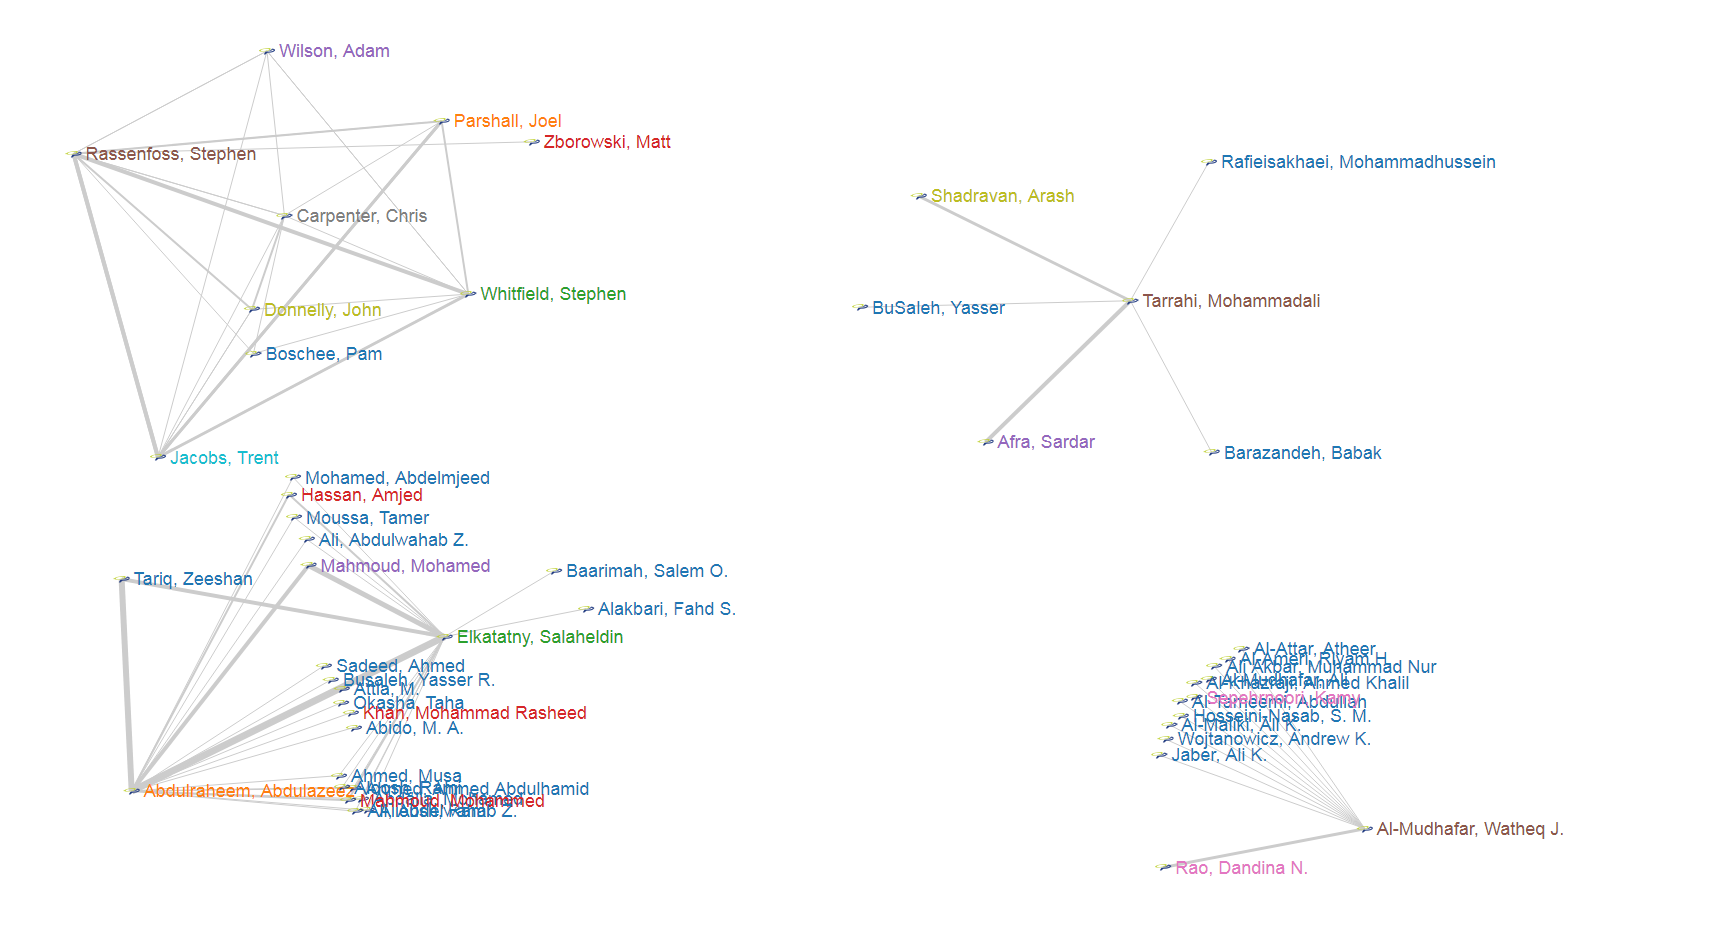
\includegraphics[width=0.95\textwidth]{rev1}
	\caption{An example of co-authorship graph.}
	\label{fig:rev1}
\end{figure}

\chapter{Object and methods}
\label{cha:objectandmethod}
The emergence of digital ecosystems is the result of the natural development of scientific cooperation and information technologies. 
The purpose of digital ecosystems is to increase the efficiency of communication between internal and external agents to support business. 
There are two broad definitions of the concept of digital ecosystems in the literature. 
The first comes from a structural and functional perspective that sees the digital ecosystem as an open network environment for effective interaction. The second, on the contrary, view the digital ecosystem as an open cluster of loosely coupled components, in which each agent is proactive for its benefit (Figure \ref{fig:om0}).

\begin{figure}[ht]

	\centering
	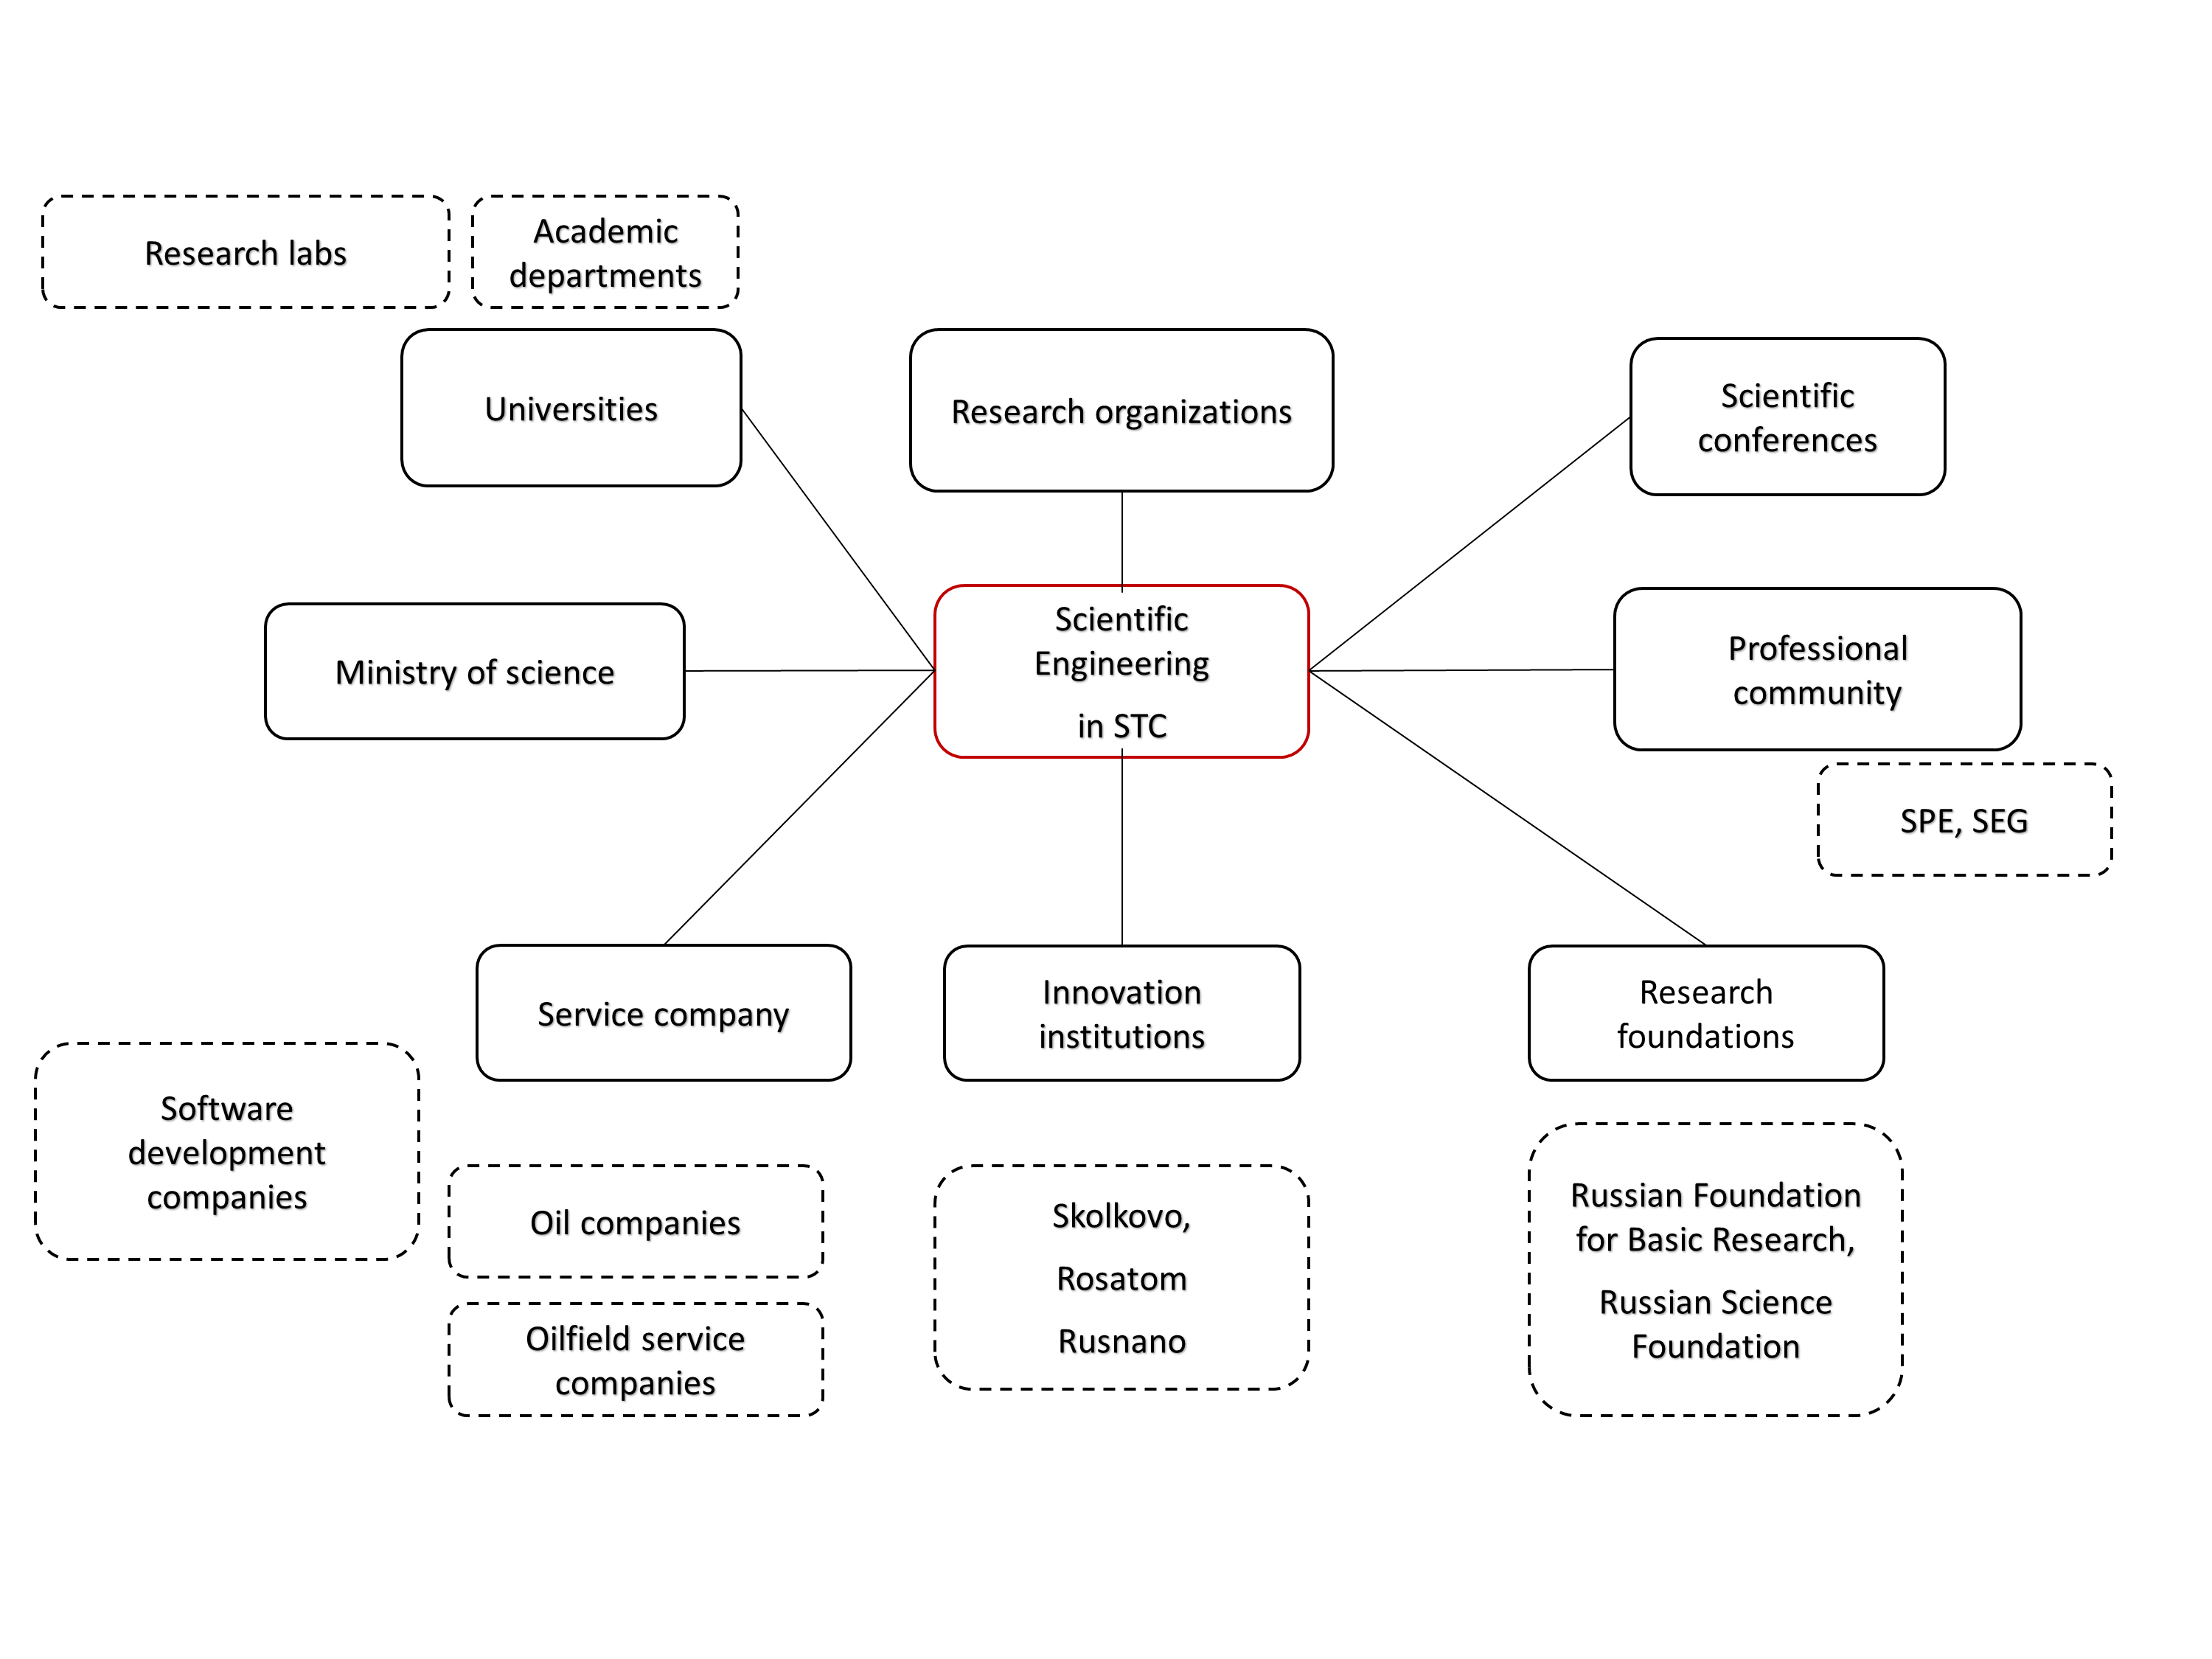
\includegraphics[width=0.95\textwidth]{se_eco_eng}
	\caption{The ecosystem science engineering.}
	\label{fig:om0}
\end{figure}

The concept of ``digital artifacts'' came into use together with the idea of the digital ecosystem. 
In a broad sense, digital artifacts are synonymous with any information output from the digital ecosystem. 
By their informational nature, digital artifacts can be preserved or destroyed. 
Both the preservation and the destruction of the original digital artifact are modified. In the historical perspective, digital objects can be studied, as well as any other products of human activity.

Digital ecosystems can be considered at the macro level (country, industry) and the micro level (Corporation, a group of companies, individual enterprise, Department). 
Digital artifacts can also exist at different levels.

One example of digital artifacts at the micro level is knowledge distribution systems (KDS) in oil and gas companies.
A knowledge distribution system is a framework that helps coordinate the processes of management and exchange of knowledge in the field of oil exploration and production within the Gazprom Neft group to solve technological and production problems in decision making.

KDS is designed to set up the processes of collecting, processing and propagating knowledge to maximize the benefits of the company's practices and technologies. 
KDS is implemented in the form of an information system with several subsystems that help to obtain the necessary information on various aspects of work at the field.

KDS systematically provides information on the best practices applied in Gazprom Neft in the field of exploration and production. 
The system allows the user to carry out a comparative analysis and selection of optimal technical solutions by the necessary criteria. It also stores data on all tests of new equipment conducted within the company, which allows the most effective implementation of new equipment and technologies at any field within the company.

The most significant contribution to the development of KDS is made by experts of the Scientific and Technical Center. 
They form a big structured knowledge database in various fields of Geology, exploration, and production, to which all Gazprom Neft employees have access. 
KDS is one of the tools to create an innovative climate within the company, necessary for the development of new, more efficient technologies for oil exploration and production

\section{Modeling of socio-technical objects}

The modern paradigm of scientific research is that real objects are replaced by their simplified representations, abstractions, selected so that they reflect the essence of the phenomenon, those properties source objects that are essential to solving the problem, which was staged.
An object that is built as a result of simplification, called a model.

Models can be classified according to different characteristics: dynamic and static, discrete and continuous, stochastic and deterministic, simulation and analytical. 

Statistical models operate on characteristics and objects that do not change over time. 
In dynamic models, the change in model parameters over time is significant.
Statistical models are dealing with the equations of balance type, steady-state processes, with marginal characteristics.
Simulation of dynamic systems is to simulate the rules of transition from a particular state to another over time.

Models whose state changes continuously over time are called continuous models. 
Models in which transitions from one state of the system to another occur instantly at separated moments of time are called discrete.

Stochastic models, unlike deterministic ones, take into account the probabilistic nature of the system parameters.

In analytical modeling, the processes of the functioning of the system under study are reflected as algebraic, integral, differential equations and logical relations, and in some instances, the analysis of such associations can be performed using analytical transformations.

In simulation modeling, the structure of the simulated system -- its connections and subsystems -- is directly represented by the structure of the model, and the process of functioning of subsystems in the form of equations and rules that bind the variables are simulated on the computer.

Computer systems for predictive modeling (also called engineering decision support systems) with computer-aided design systems have long been used to automate the work of the design engineer and improve the quality of decisions that are made. 
But until the beginning of the XXI century in predictive modeling used exclusively mathematical models based on the principles of physics, describing the physical phenomena and processes that occur in the operation of the object, complex partial differential equations with boundary conditions. 
In meaningful situations for such equations neither theorems on uniqueness and existence of the solution, nor the nature of the dependence of the solution on boundary conditions and parameters are unknown.
Numerical methods for solving these equations have significant computational complexity and the calculations themselves, and the preparation of initial data and computational grids.
Because of this, the possibility of using these models in the design of complex objects is significantly reduced, especially at the stage of conceptual or preliminary design, when a significant number of different solutions are considered, and the price of a solution that is chosen incorrectly is extraordinarily high. 
An essential part of predictive modeling is simulation modeling, which is used to study complex information and telecommunication systems.

\subsection{A posteriori and a priori approach to research}
Considering the possibilities of a posteriori and a priori approach to research, the author tends to give priority to the experimental study of this phenomenon, and then find out which of the theories can form the basis for further deepening in the study of the phenomenon of co-authorship.

Modern possibilities of direct simulation modeling have become so convenient for computational experiments that for the initial approach to the study of complex social phenomena can quickly give the researcher a significant understanding of their nature. The formalism of the mathematical model, in this case, does not abstract into the world of Greek letters but brings closer to understanding the generic features of the object under study.

The model seeks to describe the system for which it is created. 
But note that the creation of a model for a complete description of the social system is not a correct statement of the problem. 
The full model of the social system will be as complex as the social system itself. 
Let us formulate the following definition of the social system model (\ref{defi:so1}):

\begin{defn}
	\label{defi:so1}
The $\mathbb{M}_{\Omega}$ model of the social system $\Omega$ can be used to determine the characteristics $Z$ with given accuracy $\delta$.
\end{defn}

Thus, the model aims to obtain answers to a set of questions. 
These questions are implicitly present in the analysis process, and therefore they guide and guide the creation of the model. This indicates that the model will have to answer these questions with a given degree of accuracy.
If the model does not answer all questions or its answers are not accurate enough, it is said that the model has not achieved its goal.

Agent-based modeling involves simulating the performance of the system by configuring the behavior of individual agents. 
Based on the results of the behavior of individual individuals, a complex picture of interactions is formed.
The agent modeling method is used in addition to the system dynamics method, which simulates the behavior of the whole system.

Agent modeling software algorithms are developed in several information systems, in particular, Anylogic and NetLogo.
These information systems are used to solve practical problems,  in Social Sciences, including Economics and Sociology. 
An essential task of agent modeling is to include information about the interactions of agents with each other since in some social systems it is the complex structure of the communications of individual agents that lead to more complex macro-states. 
Agent-based modeling is used to study the dynamics of social networks and the mutual influence of exogenous and structural characteristics on each other.

Model for the study of the interaction of agents in the process of creating scientific articles has been implemented by the author in the software environment of agent-based modeling AnyLogic is based on Java language. 
In AnyLogic environment, certain rules of behavior are prescribed for each agent – heuristics, individual strategies.
After all the rules of behavior are prescribed for each of the agents, a series of simulations is started.
Agent modeling software environments are used to predict collective behavior, mass events, educational process, and many other social processes.

The method of simulation based on internal states and actions was used to model the processes in this study.
The main advantage of this approach is the ability to conduct a computer experiment to understand the behavior of the system as a whole by adjusting the state graphs and actions of decentralized individual agents. 
Thus, the result was a database of agent behavior for the study of processes.

Within the framework of the above methodology, the following research questions were formulated:
\begin{enumerate}
	\item To what extent does the scientific paper reflect the conducted research? Is it possible to judge the quality of research on published research?
	\item What are the social mechanisms for bringing together researchers to conduct research? What types of competencies and to what extent do they influence such integration?
	\item How does the time of research depend on the number of researchers involved? Are there natural limitations on the number and composition of research teams?
	\item What are the heuristic algorithms of handling researchers with the publishers and programme committees of conferences? Are there basic behavioral strategies? If it is possible to identify and simulate basic strategies?
	\item Are time management approaches applicable to R\&D? How effective is the consideration of research as a project activity?
	\item What is the maturity model of the research organization concerning research? To what extent is it possible to determine the degree of maturity of a research organization based on the analysis of scientific articles published by it?
	\item What is the structure of the processes that make up the research activity? How appropriate process approach to the study of research activities? There are indicators of research activities, reflecting the characteristic structure of its constituent processes?
\end{enumerate}

\subsection{Theory of simulation}

Simulation modeling is a method of research in which the system under study is replaced by a model that accurately describes the real system with which experiments are conducted to obtain information about this system.

The purpose of the simulation is to obtain approximate knowledge about a specific parameter of the object, without direct measurement of its values. 
This is necessary when the direct measurement is not possible or is more expensive than the simulation.
At the same time, to study this parameter, it is possible to use other known settings of the object and the model of its design.
Assuming that the design model accurately describes the object, the authors suggest that the statistical distribution of values of the parameter modeling of the object, obtained during simulation, will to some extent coincide with the statistical distribution of values of the parameter of the real object.

Areas of application of simulation modeling are:

\begin{itemize}
	\tightlist
	\item Agent-based modelling
	\item System dynamics
	\item Discrete event simulation
	\item Dynamic systems
\end{itemize}

Next, we consider in more detail System Dynamics.

\subsection{System Dynamics}

This approach was developed and proposed by Jay Forrester in the late 1950s as a study of information feedbacks in industrial activity to show how organizational structure, gains (in policies) and delays (in actions and decision-making) interact, influencing the success of the enterprise.

Applications of system dynamics also include urban, social, environmental systems. Processes that occur in reality are represented in System Dynamics regarding drives (stocks, for example, material objects, people, knowledge, money), flows between these drives and information that determines the value of such flows.
System Dynamics is abstracted from certain events and objects and assumes an aggregate view of processes.
It focuses on the politicians who manage these processes.
By modeling in the style of System Dynamics, you represent the structure and behavior of the system as a set of interacting negative and positive feedbacks and delays.

\subsection{Model building principles}

Set of system-dynamic models can describe a socio-economic system. 
The choice of factors to be included in the model depends on the questions to be answered.
But in broader case, the base of the model cannot be limited to any narrow scientific discipline.
It is necessary to include in the model economic, organizational, legal, technical, labor, psychological, historical and monetary factors.
All of them should find their place in determining the interaction of the elements of the system. 
Any factor can have a decisive influence on the behavior of the system.

Typically, 30 to 3,000 variables are included in the most important models that meet management requests.
The lower limit is close to the minimum, reflecting the main types of system behavior that interest decision makers.
The upper limit is limited by our ability to perceive the system and all its interactions.

Particular attention should be paid to such aspects of the system under study as:

\begin{itemize}
	\tightlist
	\item time dependencies,
	\item backward dependencies,
	\item distortion of information.
\end{itemize}

When building a model, its variables must correspond to the variables of the system being modeled and be measured in the same units.
For example, the flow of goods should not be measured in monetary units, but in physical units. 
Cash flows are considered separately.
Cash and commodity indices connected with prices.
Goods cannot be presented as corresponding monetary amounts, otherwise, the value of prices and the fact that the movement of money is not synchronous to the flow of goods will not be taken into account.
Orders for products are not products, shipped products are not equal to invoices, and the invoices are not equivalent to cash.

The economic system model should use actual prices rather than indexed or quoted prices.
Actual prices and their fluctuations lead to critical psychological consequences, for example, when determining the number of wages.

The system-dynamic model does not have to be stable.
Among the existing socio-economic systems, certain are unstable in mathematical understanding.
They do not tend to the equilibrium state even in the absence of external disturbances.
Social systems are highly non-linear and most of the time counteract the restrictions that are associated with a lack of labor, overcoming inflation, reduction of monetary resources, the decline in business activity, lack of means of production.

\subsection{Stages of computer simulation}
In addition to the principles, there are typical stages of computer simulation. 
Typically, it includes the following steps:

\begin{itemize}
	\tightlist
	\item Understanding the system: understanding what is happening in a system that subjects to the analysis: what is its structure, what are the processes leak in it.
	\item Formulation of the purpose of system modeling: a list of tasks that it is supposed to be solved utilizing the future model. List of weekends and  the input parameters of the model, the data source listing, the criteria completeness of future research.
	\item Development of the conceptual structure of the model:  the structure of the model, the composition essential processes to be displayed in the model,  fixed level of abstraction for each subsystem of the model  (list of assumptions), description of control logic for subsystems.
	\item Implementation of the model in the modeling environment: implemented subsystems, their behavior, their parameters, performed the logic of subsystems communication.
	\item Implementation of the animated representation of the model: model view, user interface.
	\item Validation of model implementation: the belief that the model correctly reflects the processes of the real system that are required to analyze.
	\item Calibration of the model: fixation of parameter values, the equations coefficients, and distributions of random variables that reflect situations for which the model will be used.
	\item Planning and implementing a computer-based experiment: results simulations -- tables, graphs, databases, models that correspond to put the question.
\end{itemize}

In addition to the stages of modeling, it is necessary to consider the principles of data collection required for the experiment. 
This will be discussed in the next subsection.

\subsection{Data acquisition}

Simulation is a statistical experiment.
Its results should be based on appropriate statistical tests: confidence intervals and methods for testing hypotheses.
To perform this task, the obtained observations and simulation experiment must meet the following requirements:

\begin{enumerate}
	\tightlist
	\item \textbf{Observations have stationary distributions, that is, distributions do not change during the experiment.}
	The results of observations on the model are dependent on the duration of the simulation period.
	The initial period of unstable behavior of a model is usually referred to as transitional.
	When the results of the simulation experiment stabilize, the system goes into a steady state.
	The longer the run time of the model, the higher the chance of achieving a steady state.

	\item \textbf{Observations are subject to normal distribution.}
	This requirement can be fulfilled if we involve the central limit theorem that states that the distribution of the average sample is asymptotically normal, regardless of the distribution of the general the aggregate from which the sample was taken.
	
	\item \textbf{Observations are independent.}
	The nature of a simulation experiment does not guarantee independence between consistent observations of the model. 
	But the use of samples averages for the presentation of individual observations gives the opportunity to decrease a problem that is associated with a lack of independence.
\end{enumerate}

There are three most common methods for collecting information during simulation modeling:
\begin{enumerate}
	\tightlist
	\item \textbf{Subinterval method.}
	Let us consider a simulation of $n$ observations with a duration $T$. 
	The information relating to the transient state is cut off according to this method, and the rest of the simulation results is divided into $n$ equal parts.
	The average value of the desired value within each subinterval is used as the only observation.
	The advantage of this method is that the influence of non-stationary conditions is reduced.
	The disadvantage is that successive groups with a common border are correlated, which leads to a failure to fulfill the assumption of independence.

	\item \textbf{Repeat method.}
	In this method, each observation is represented as an independent model run, in which the transition period is not taken into account.
	The calculation of the average sample values for each group is carried out in the same way as in the subinterval method.
	In this case, the standard formula for dispersion is applicable, since the groups are not correlated with each other.
	The advantage of this method is that each simulation run of the model is determined by its sequence of random numbers from the interval, due to which the statistical independence of the obtained observations is provided.
	The disadvantage is that the initial transient conditions can strongly influence all observations.
	
	\item \textbf{Cycle method.}
	This method can be considered as an extended version of the subinterval method.
	In this method, we tried to reduce the effect of autocorrelation by selecting groups to provide the same initial conditions for each of them.
	The length of the queue can be considered as a variable. 
	Then each group should start at the moment when the queue length is zero.
	In contrast to the subinterval method, in the method of cycles, the length of the intervals of each group may be different.
	The disadvantages of the method include a smaller, in comparison with the subinterval method, the number of observations obtained at a given run length.
\end{enumerate}

Simulation is a reasonably flexible research tool that can be effectively used in the analysis of complex systems.
Its disadvantage is that any result obtained by simulation modeling is subject to experimental errors and must be verified by statistical tests.
The task of obtaining observations using simulation modeling, which is both representative and independent in stationary conditions, is somewhat tricky.
The use of specialized data collection techniques can mitigate these difficulties.

\subsection{The use of simulation models in historical research.}

Theoretical and methodological problems of application of simulation models have not yet been developed.
There are different opinions about the possible use of simulation models in history, but there is a great interest in their application.
The existing experience of their practical construction makes it possible to identify three types of tasks that can be solved on their basis:

\begin{itemize}
	\tightlist
	\item modeling alternative, that is subjectively and objectively possible, but unrealized in practice historical situations in order to characterize the real course of development more deeply;
	\item building models of counterfactual (really non-existent) historical situations that are constructed by the historian in order to use these models as a benchmark for assessing real historical reality;
	\item imitation of historical phenomena and processes, for the collective characteristics and reflective-measuring modeling of which there is no necessary concrete historical data.
\end{itemize}

In recent years, significant success has been achieved in the field of creating models of social history.
The models currently available can be divided into three groups:

\begin{enumerate}
	\tightlist
	\item model-concepts based on identifying and analyzing general historical patterns, representing them in the form of cognitive schemes describing the logical connections between various factors influencing historical processes (J. Goldstein).
	These models have a high degree of generalization, but have not a mathematical, but a purely logical, conceptual character;
	\item particular mathematical models of the imitation type, which are devoted to the description of specific historical events or phenomena (D. Meadows, J. Forrester).
	In such models, the focus is on careful consideration of the description of the factors of the processes that influence the phenomena under consideration.
	The applicability of these models is usually limited to a rather narrow space-time interval; they are `` tied '' to a specific historical event, they cannot be extrapolated for long periods of time;
	\item mathematical models that are intermediate between these two types.
	These models describe a specific class of social processes without a claim for a detailed description of the features of each specific historical case.
	Their task is to identify the underlying patterns that characterize the processes of the type in question.
	By this, these mathematical models are called primary. 
\end{enumerate}

\section{Model of the process of publishing scientific articles}

All researchers were faced with the fact that publishing the results of a study is almost as tricky as performing the study itself.
Consider the process of publishing research results in detail and analyze the possibilities of its acceleration and simplification for the authors.
The starting point for our analysis will be a sharp text describing, from researchers, the result of their research work.
Traditionally, this text is called a manuscript.

In the modern world, the speed of publication of manuscripts is a critical factor for the growth of the country's scientific contribution to international science.
Publication of articles requires a wide range of administration and communication skills from researchers, which are not always characteristic of scientists.
The need for these individual authors to acquire these skills creates the risk of losing focus on research questions and takes time away from scientists, which can be usefully spent on science.
On the other hand, by co-sponsoring people, for example, to translate articles into English or lobbying business trips to a conference, the authors blur the research profile of the organization and create so-called ``guest-authors''.

Historically, the task of a scientist is to make the result of a study accessible to the broadest range of stakeholders; this is the essence of the process of publishing research results.
The primary goal of this thesis is to explore the process of publishing a manuscript, understand bottlenecks, identify opportunities for their elimination, and suggest improvements.
Below is the research framework of the study in the form of a diagram (Fig. \ref{fig:om1}):

\begin{figure}[ht]
	\centering
	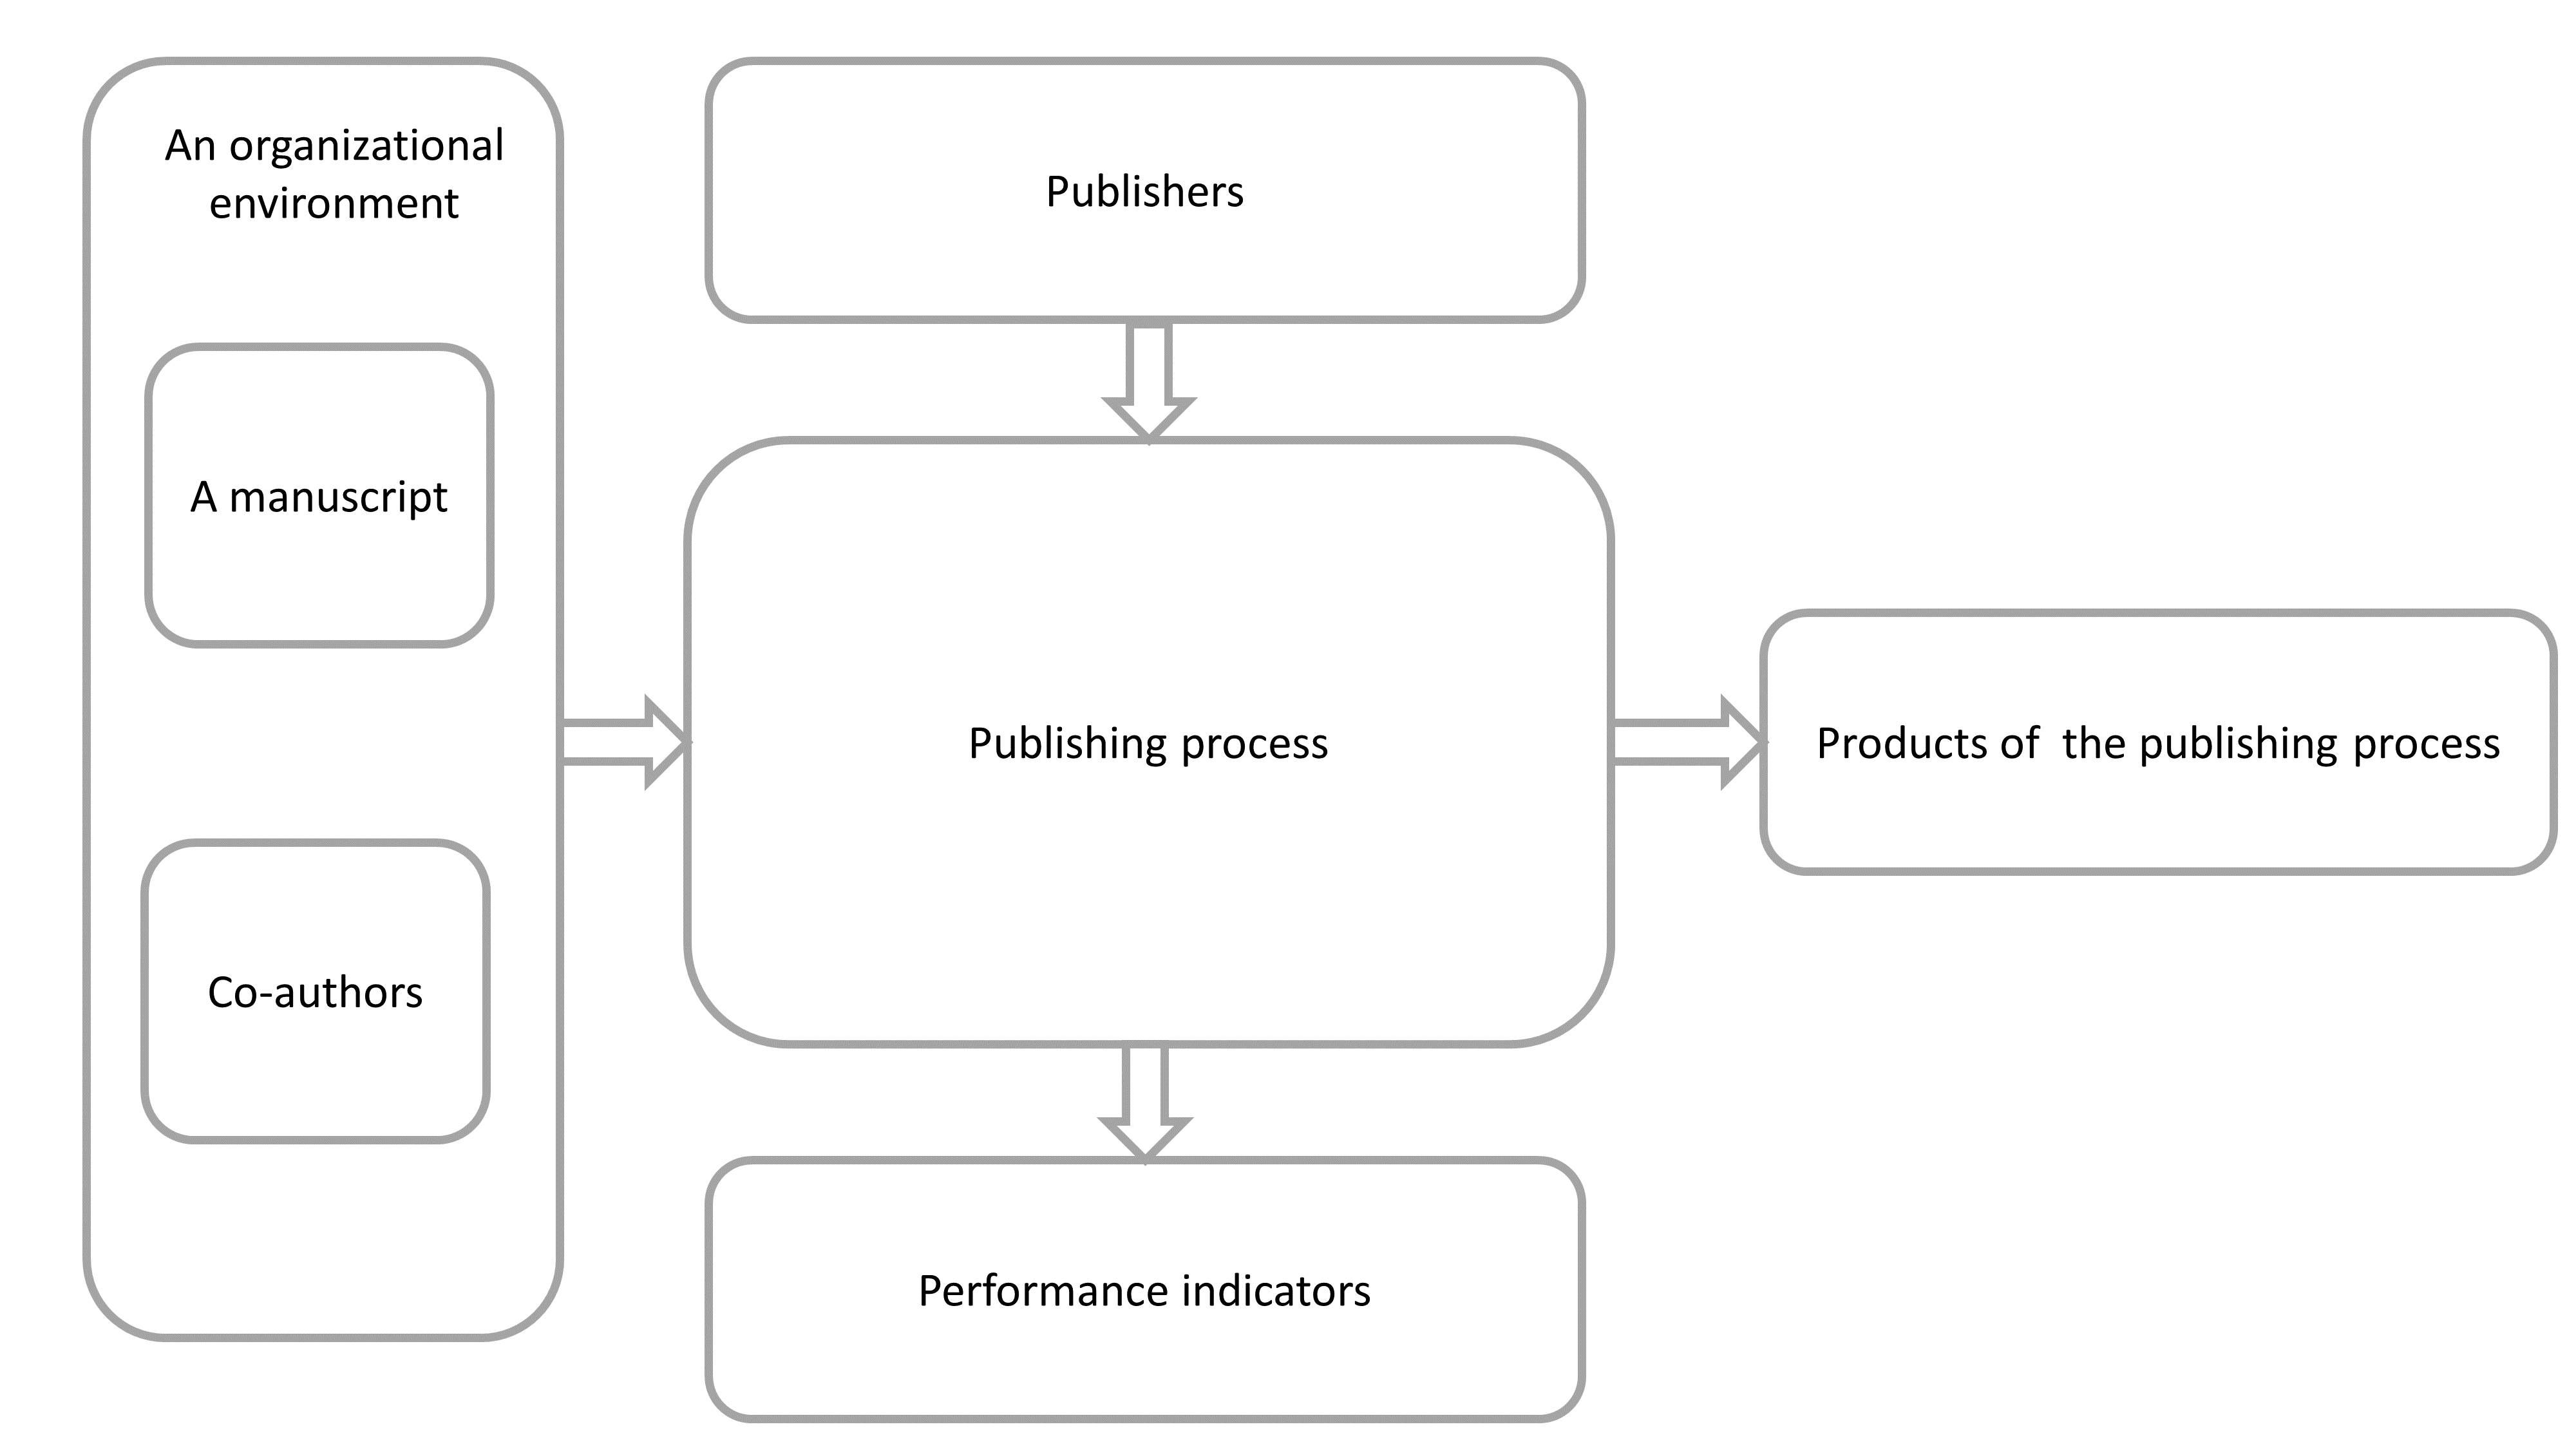
\includegraphics[width=0.8\textwidth]{om1_eng}
	\caption{The research framework for publishing processes.}
	\label{fig:om1}
\end{figure}  

As can be seen from the figure (\ref{fig:om1}), the logical framework of the study includes the organizational environment (co-authors and their manuscript), the process of publication, publishers, performance indicators and the results of publication. 
In the next subsection, each of the components of the logical framework will be discussed in more detail.

\subsection{Manuscript}
As mentioned earlier, a form manuscript is a text.
Methodologically, manuscripts are divided into the following main types:

\begin{itemize}
	\tightlist
	\item Monography, dissertation
	\item Paper 
	\item Report theses
\end{itemize}

A scientific article is a work of a small volume, usually from five to twenty pages. 
The content of scientific articles is divided into three types: theoretical articles,  practical articles, and methodical articles. 

Practical articles are devoted to logical experiments and real experience. 
Further, it will be considered this type of manuscripts.

\subsection{Co-authors}
The most study is done by research teams, not by single authors. 
That is why manuscripts are also written as a result of collective work.
According to the study \cite{kradoya2016structure}, in the oil and gas industry, the distribution of the number of co-authors has the form shown in the Figure \ref{fig:om2}.

\begin{figure}[ht]
	\centering
	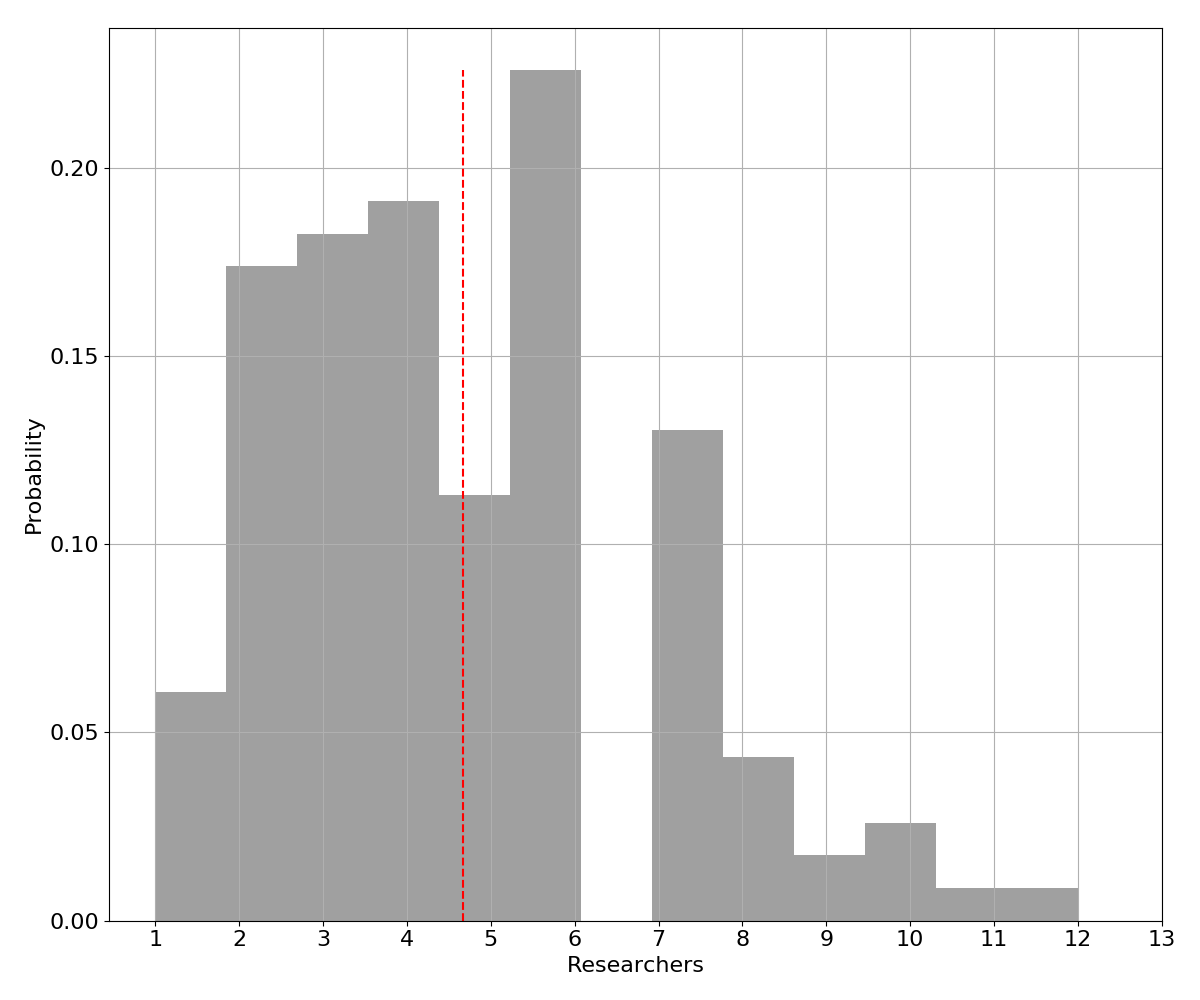
\includegraphics[width=0.6\textwidth]{om2}
	\caption{Distribution of the number of co-authors of scientific articles in the oil and gas industry.}
	\label{fig:om2}
\end{figure}  

The figure \ref{fig:om2} shows the normal distribution of the number of co-authors. The red line indicates the average value: $4.67$. 
The standard deviation of the distribution is $2.28$.

\subsection{Organizational environment}

Research is carried out by employees of research departments. 
In the oil and gas industry, such units may belong to specialized institutes, scientific and technical centers, service organizations and other participants of the ecosystem. 
Thus, the co-authors work in an organizational environment. 
The organizational environment largely determines the communication between co-authors, which is vital in our research.

\subsection{The publishing process}

The publishing process consists of two types of actions:
\begin{itemize}
	\tightlist
	\item Interaction of co-authors with the publisher;
	\item Interaction between co-authors;
\end{itemize}	

The object of both actions is the manuscript and additional related materials: questionnaires, presentations, letters, reviews.
The main task of interaction with the publisher is to meet the conditions for the publication of the article in this edition. 
Usually, the requirements for authors are indicated on publishers' websites and may differ.  
Co-authors' interactions during the publication process include the following:

\begin{itemize}
	\tightlist
	\item Creating a list of possible publishers,
	\item Study of specific topics required by publishers,
	\item Defining the time limits for the submission of the manuscript,
	\item Preparation of the manuscript revision plan to meet the requirements of publishers,
	\item Collection of related documents according to the requirements of publishers,
	\item Preparation of presentation for the report (required for conferences)
	\item Make an oral presentation (business trip)
	\item Confirmation of authorship in the science community and citation indexes.
\end{itemize}

The most significant are the publishers recommended for publication by the Higher Attestation Commission (HAC). 
The ``list of peer-reviewed scientific publications'' of the HAC as of 20.09.2017 contains 2172 magazines. 
We will choose publishers by one, the closest to the oil and gas industry specialty-25.00 ``Earth Sciences''.
There are 147 such magazines. 
Then the author of the study proposed the following sequence for data collection (Fig. \ref{fig:om2_1} ).

\begin{figure}[ht]
	\centering
	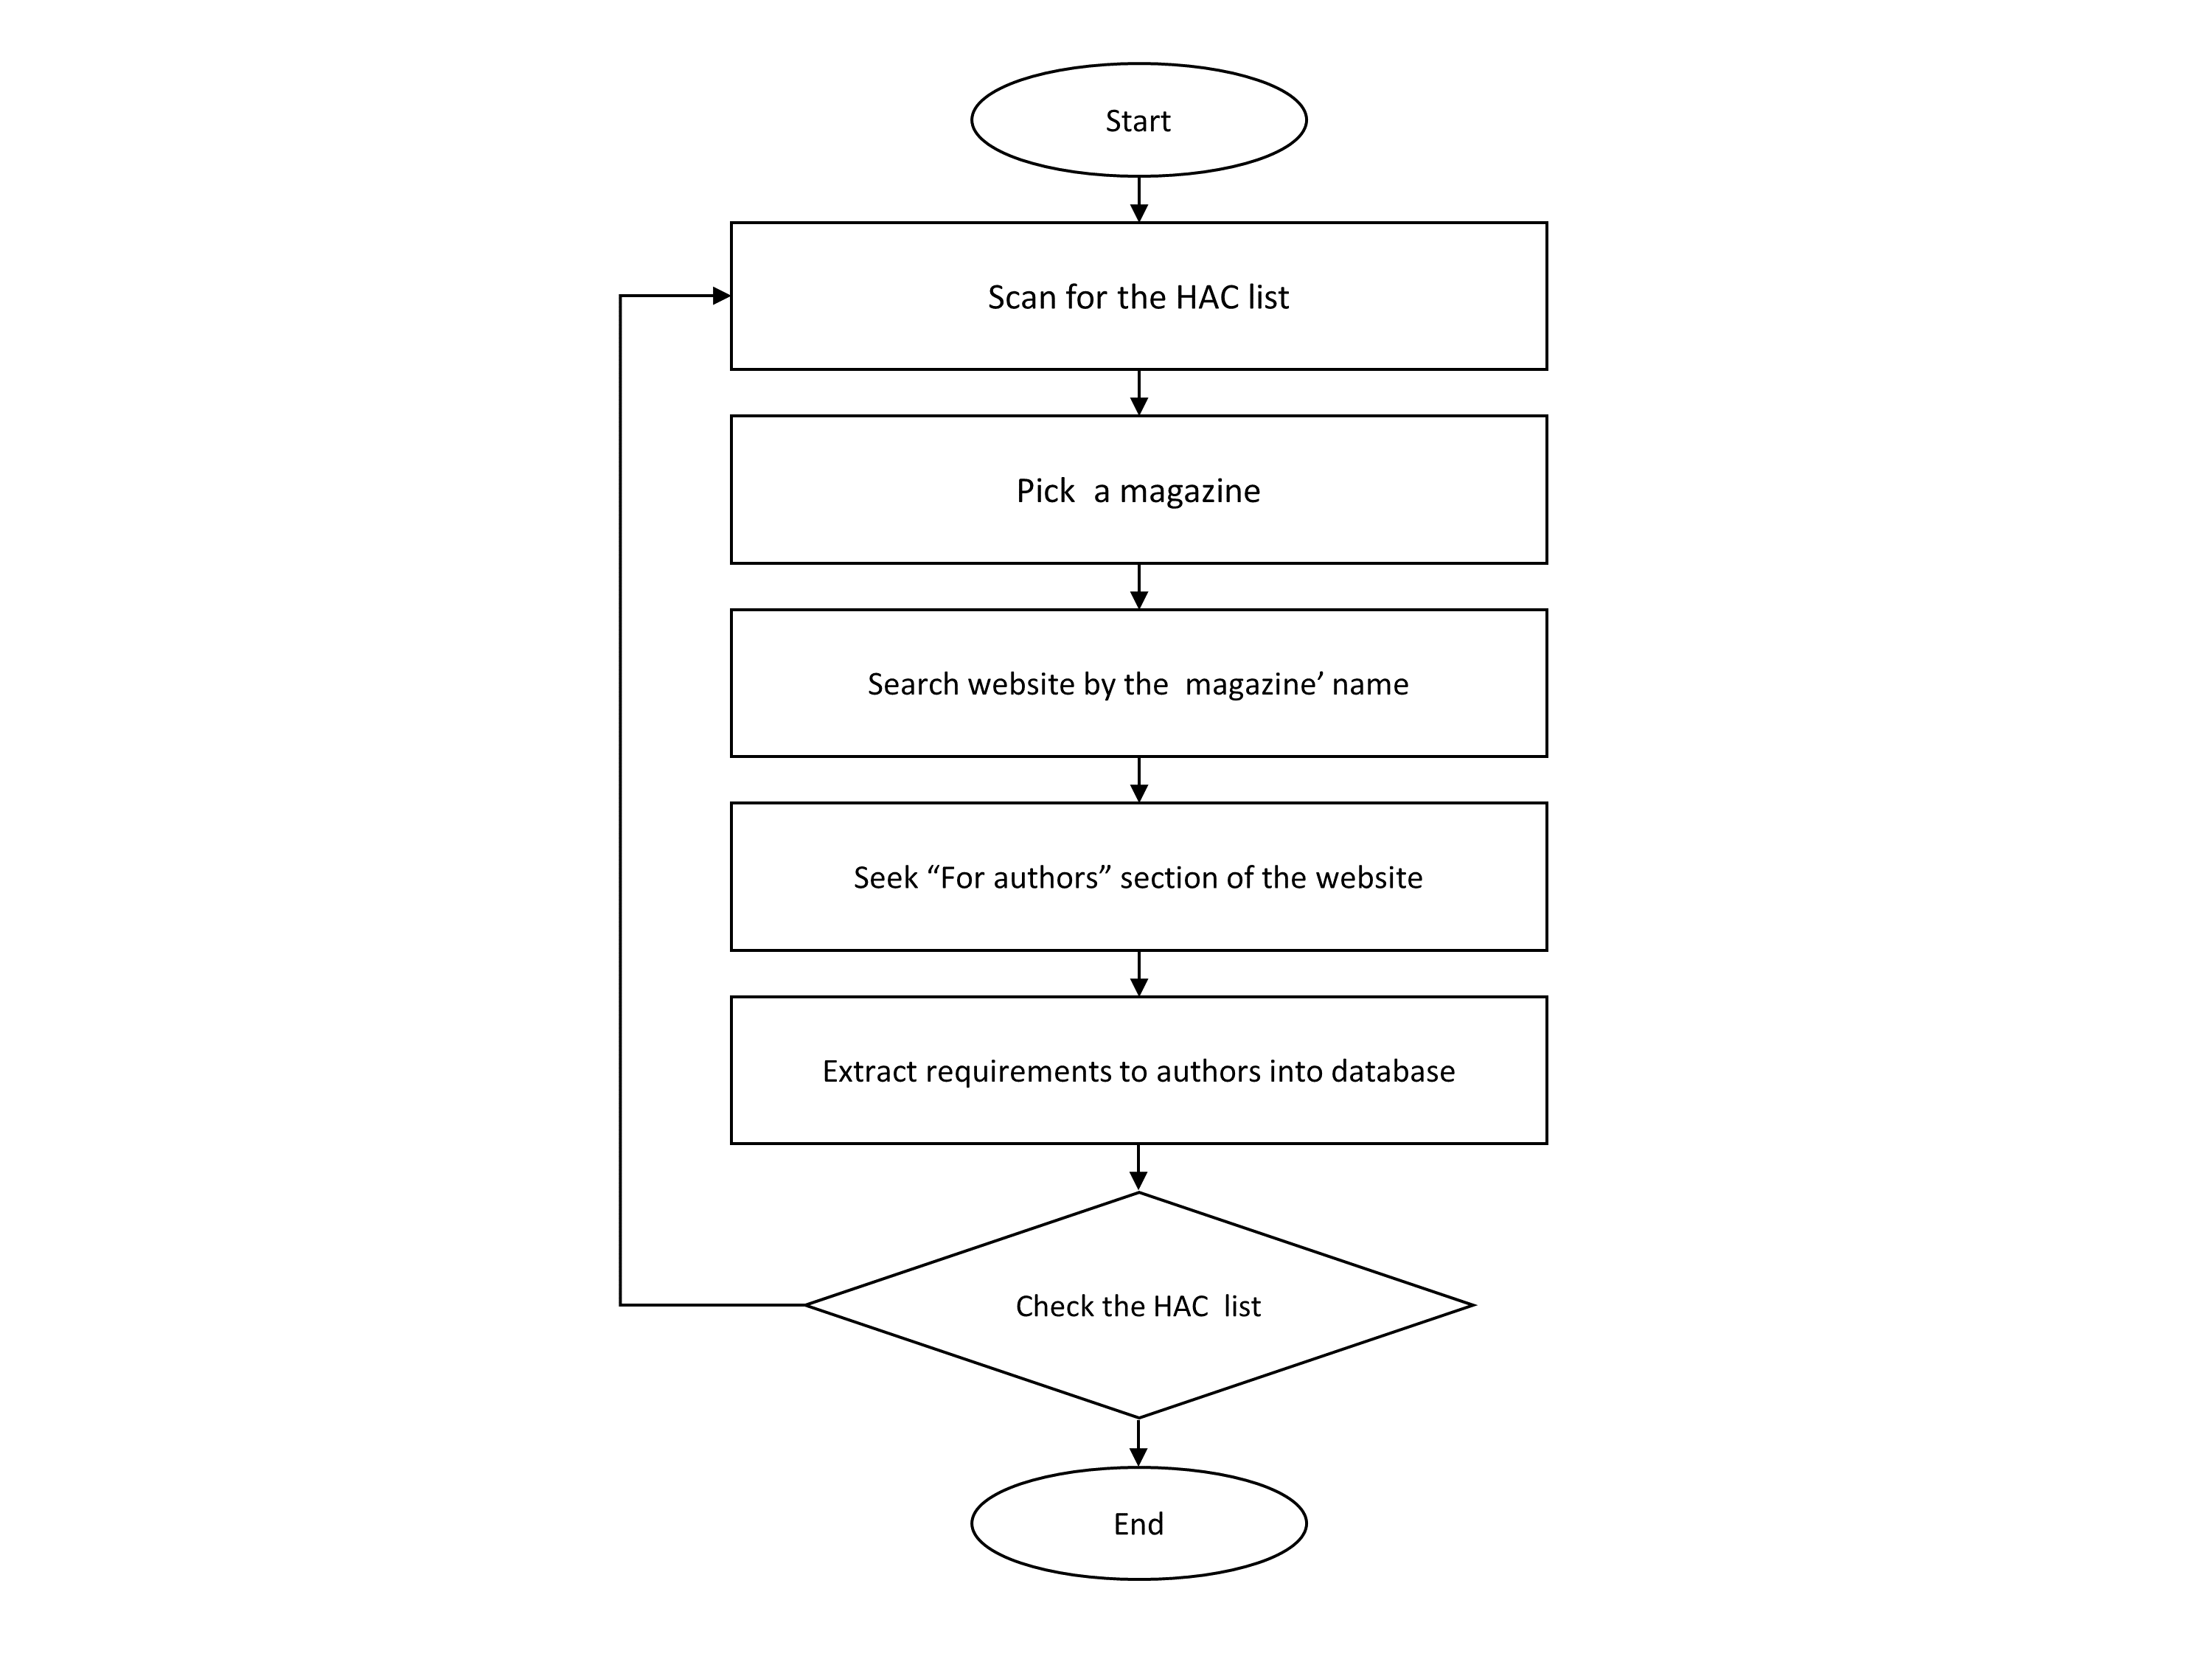
\includegraphics[width=0.99\textwidth]{om2_1_eng}
	\caption{Algorithm for author' requirements collection.}
	\label{fig:om2_1}
\end{figure}  

Let's use the results of research \cite{mazov2015russian} to select publishers with the highest publication activity and impact factor on international abstract databases. 
The list contains 16 journals. 
All 16 journals have standard rules for authors developed by the publisher MAIK "Nauka/Interperiodika".
Each edition has its allowable volume of publications, due to the number of articles in one issue and the number of issues per year.
The more manuscripts the publisher receives, the higher the competition for the right to be published.

\subsection{The results of the publication.}

The result of the publication is a real contribution to science. 
The problem of maximizing the availability of research results in the Internet era can be solved by using Internet resources. 
Here are just some ways to increase the audience:

\begin{itemize}
	\tightlist
	\item The international scientometric databases (Scopus, WoS), 
	\item Digital libraries (for example, eLibrary.ru, OnePetro.org),
	\item Assignment of the digital object identifier (DOI) to a scientific article, 
	\item Linking a scientific article to an author in online communities of scientists (for example, ResearchGate),
	\item Publication of the material in open libraries (e.g., aRxiv.org),
	\item Binding an article to a scientist identification number (e.g., ORCID, SPIN),
	\item Citation indexes (e.g., Russian Science Citation Index).
\end{itemize}

Citation index, for example, the Russian Science Citation Index (RSCI), is one of the most common scientometric indicators in Russia and is used for formal evaluation in the scientific community.
Alternatives to the citation index are expert evaluation and evaluation of the impact factor of scientific journals.
In-depth methods of bibliometric analysis provide an opportunity to consider the contribution of the author from different points of view.
Much attention is paid in particular to the analysis of publications using co-authorship graphs, discussed further in \ref{sec:coat}. 
An example of the co-authorship graph is shown in the figure (Fig. \ref{fig:om3}).

\begin{figure}[ht]
	\centering
	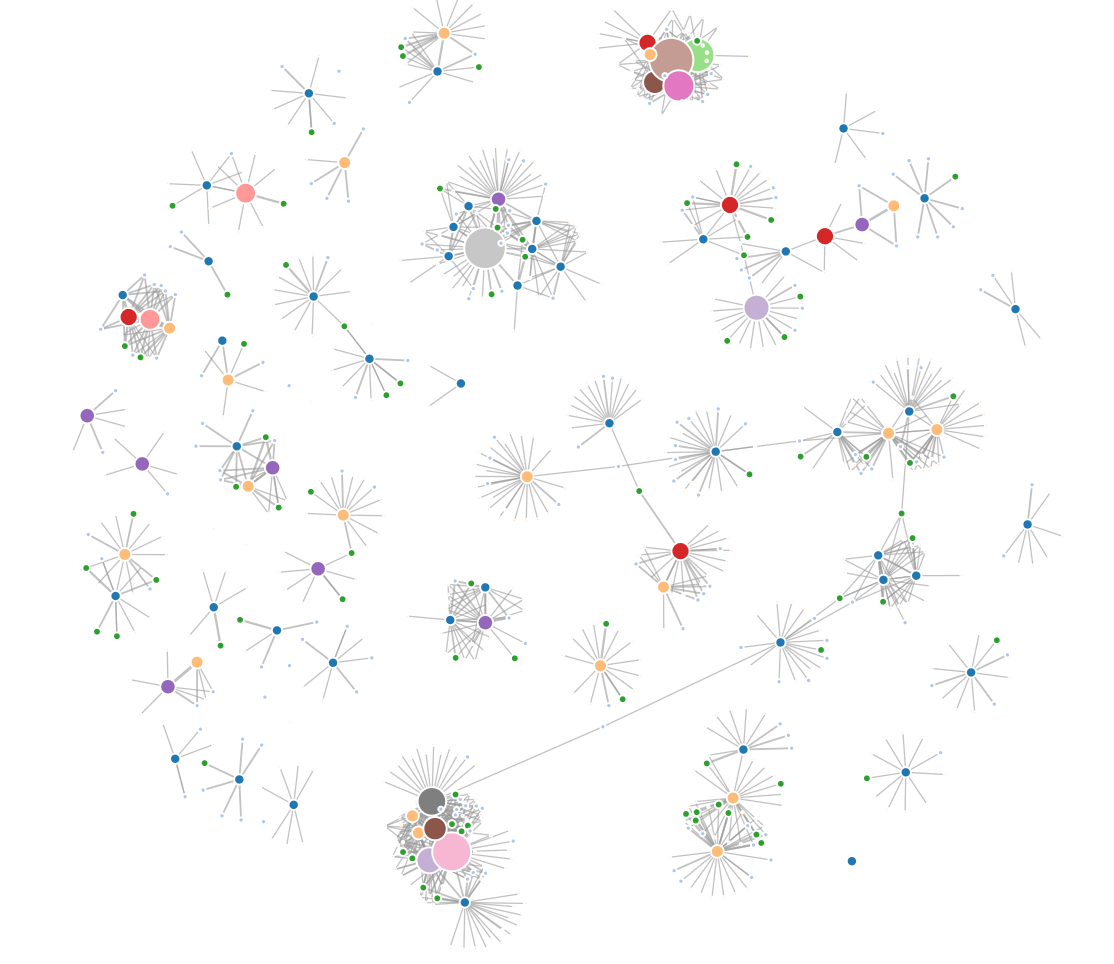
\includegraphics[width=0.8\textwidth]{om3}
	\caption{An example of co-author graph for keyword \textit{Oil rims}}
	\label{fig:om3}
\end{figure}  

Graphs of co-authors allow visually identify the most important scientists on the consideration subject.
For example, in the figure \ref{fig:om4} we can see such a cluster.

\begin{figure}[ht]
	\centering
	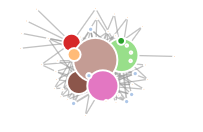
\includegraphics[width=0.40\textwidth]{om4}
	\caption{A fragment of the graph of co-authorship of the keyword Oil rims.}
	\label{fig:om4}
\end{figure} 

On the figure \ref{fig:om4} only nodes belonging to Professor Rahim Masoudi are depicted.

The principle of construction of co-authorship graphs is to classify the number of publications on the selected keyword to the vertices (authors), and the facts of co-authorship to the edges of the graph. 
This principle of graph construction allows to analyze it using social network analysis (SNA) methods.

\subsection{Performance indicators}
Performance indicators of the publication process need to give an integrated description of the process and allow to compare various implementations process. 
The table \ref{tab:om1} shows the most valuable  performance indicators.

\begin{table}[H]
	\centering
	\caption{Performance indicators of the publishing process.}
	\label{tab:om1}
	\resizebox{\textwidth}{!}{%
		\begin{tabular}{|l|l|}
			\hline
			\textbf{Performance indicator} & \textbf{Description} \\ \hline
			Efficiency of publications & The ratio of the number of published manuscripts to the total number of written manuscripts  \\ \hline
			The share of published manuscripts per author & The ratio of the number of published manuscripts to the number of authors \\ \hline
			The proportion rejected by the publishers of manuscripts per author & The ratio of rejected manuscripts to the number of authors in the organization \\ \hline
		\end{tabular}%
	}
\end{table}

It is assumed that the process is more productive when \textit{Publication Efficiency} tends to one, \textit{Share of published manuscripts per author} increases, and \textit{Share of rejected papers per author} tends to zero.
Strategies for managing the publication process through productivity indicators are given in the table \ref{tab:om2}.

\begin{table}[H]
	\centering
	\caption{Performance management strategies for the publication process through productivity indicators.}
	\label{tab:om2}
	\resizebox{\textwidth}{!}{%
		\begin{tabular}{|l|l|l|}
			\hline
			\textbf{Performance indicator} & \textbf{Maximum productivity} & \textbf{Minimum productivity} \\ \hline
			Publication Efficiency & tends to one & tends to zero \\ \hline
			Share of published manuscripts per author & Increases & Decreases \\ \hline
			Share of rejected papers per author & tends to zero & Increases \\ \hline
		\end{tabular}%
	}
\end{table}

Note that these productivity indicators do not characterize the quality of the scientific article.
In this study, the author does not set the task of assessing the quality of scientific work.

By the above-stated methodical principles, the model of the process using system dynamics can be constructed.

\section{Theory of surrogate modeling}

The surrogate model is the basis of a new direction of modeling in engineering.
It is a mathematical method of drawing up a model based on the results of tests and computational experiments conducted with various objects of the same class.
In some cases, surrogate modeling is the only way to solve the engineering problem.

The task of surrogate modeling is to optimize the original complex function in such a way as to minimize the calculation area and minimize it. 
Creation of the surrogate model of the objective function subsequently replaces the function itself and simplify many engineering tasks.

The concept of creating surrogate models consists of the following stages:

\begin{itemize}
	\tightlist
	\item  
	Characteristics of the object $Z$, which determines the properties of an object under certain conditions, can be described in the form of the functional dependence of $Z= \Phi \left( X, Y \right)$, where the variable $X$ represents the object, and the variable $Y$ specifies the conditions of operation.
	\item
	The function $\Phi$ is unknown, and computational experiments are carried out to calculate it.
	\item
	There are a number of measurements $ \Xi = \{ X_i,Y_i,Z_i= \Phi_i \left( X_i,Y_i \right), i \in \mathbb{R} \} $, where $Z_i= \Phi_i \left( X_i, Y_i \right) $ of the characteristic of $Z$ obtained by $M_i$ for object with description $X_i$, in the framework of the $Y_i$.
	\item
	Over a well-known $\Xi$ with the help of certain mathematical methods for the analysis and processing of data is a function of $\Phi^s \left( X,Y \right)$ whose value is taken as the approximate value of the characteristics $Z$ of the object with the description of $X$ in terms of operation $Y$.
	\item
	If all values in the set $\Xi$ are obtained using the same model $M$ and $\Phi^s (X,Y) = \Phi^m \left( X,Y \right)$, then the constructed function $\Phi^s$ can be considered as a ``substitute" (surrogate) for the function $\Phi^m$.
\end{itemize}

Surrogate modeling has been successfully applied in such areas as electrical engineering, oil, water management, military, mechanical engineering, and chemical industry.

The use of surrogate models is also indispensable in construction to optimize aerodynamic contour to identify the optimal shape of unique civil structures, such as high-rise buildings and long-span bridges, which are surrounded by turbulent flow.

The following tasks of the oil and gas industry can also be solved using surrogate models:
\begin{itemize}
	\tightlist
	\item Surrogate reservoir model,
	\item Optimizing the location of wells,
	\item Uncertainty analysis of oil production forecast,
	\item Automatic adaptation of the basin model according to the data.
\end{itemize}

Some computational experiments use the meta-algorithm described above to solve problems in the oil and gas industry. 
For example, the hydrodynamic simulator first calculates the function values for specific nodal values of $X_i$ parameters based on the physical laws of fluid motion in a porous medium $M_i$. 
And then the function $\Phi$ specified in this numerical way is used to obtain the values of the function $Y_i$ either on a more detailed set of parameter values or for parameter values beyond the nodal values $X_i$.

One of the main reasons for the meta-algorithm described above is the construction of a surrogate model is the limitations on the speed of hydrodynamic modeling. 
In the future, when at any time any specialist of the organization will be able to vary the values of parameters in a wide range and in near real time to get the desired values of the function, the need for surrogate models is likely to disappear.
In the meantime, modeling is performed on expensive high-performance computational clusters, with the help of specialists for the times measured in hours and sometimes days for one set of parameters, there is a need for foresight data preparation that may be needed in the future.
Since the need to change the parameters can occur several times a day and demand a variety of specialists from different departments of the organization, the use of surrogate modeling is an urgent need.
The resulting surrogate model $\Phi^s$, sometimes called a proxy model, exceeds the original model $\Phi^m$ in computational power many times, that is, does not require a large number of computing resources and operates in near real time.

\section{Nonparametric models}

To understand non-parametric models let us consider a parametric model. 
A parametric model $p$ for values of $y$ dependent variables $X$ and parameters $\theta$ would be $p\left( y\vert\theta \right)$.
Finding the $\theta$ parameters using the a posteriori probability maximization methods $p \left( \theta \vert y,X \right) \longrightarrow \max_\theta $.

Optimization methods are used to find the optimal parameters of the mathematical model.
Numerical optimization methods are:

\begin{itemize}
	\tightlist
	\item Gradient and non-gradient,
	\item Robust (for optimization problems under uncertainty), 
	\item Surrogate-based.
\end{itemize}

Let's consider Bayesian optimization methods, which are most often used in surrogate and simulation modeling. In this case, the data and the model are a ``black box''.

Let the function $f \left( x \right)$ be given and we need to find $x$ at which it reaches a maximum of $f \left( x \right) \longrightarrow \max_x$. Let's add a condition under which the calculation of each value $f \left( x \right)$ is a resource-intensive task. 
This condition may occur in the following cases:

\begin{itemize}
	\item $x$ are the geographic coordinates of the well, and $f \left( x \right)$ is the amount of oil that can be extracted by drilling the well at $x$ coordinates. 
	In this case, one value of $f \left( x \right)$ is worth millions of rubles;
	\item $x$ are hyperparameters of artificial neural deep learning network, $f \left( x \right)$ is a target metric of prediction accuracy. 
	In this case, one value of $f  \left(  x \right) $will take months of work;
	\item $x$ is the medicine formula, and $f \left( x \right)$ is the efficacy of the medicine against the disease. 
	In this case, one $f \left( x \right)$ will cost the life of one test animal.
\end{itemize}

Thus, the formulation of the problem is to optimize the target function in the minimum number of attempts. 
At the same time, the use of surrogate models of the objective function allows making each optimization step less resource-intensive. 
Let us introduce the function values of the detection of $\mu \left( x \right)$ that characterizes the benefit received from the optimization of $f \left( x \right)$ when using a surrogate model $\hat{f}$. 
Value function detection is a quantitative evaluation function to minimize the number of attempts. 
Consider the following $\mu \left( x \right)$:

\begin{itemize}
	\item Maximum probability of improvement (MPI): $ \mu \left(  x \right)  = P(\hat(f \left(  x \right) ) \geq f^* + \epsilon =  \Phi \bigg( \frac{\mathbb{E}\hat{f \left(  x \right) } - f^* -\epsilon}{Var[\hat{f \left(  x \right) }]}\bigg) $, where $f^*$ - current best value.
	\item Upper confidence bound (UCB): $ \mu \left(  x \right)  = \mathbb{E}\hat{f \left(  x \right) } + \eta Var[\hat{f \left(  x \right) }] $
	\item Expected improvement (EI): $ \mu \left(  x \right)  = \mathbb{E} \max(f \left(  x \right)  - f^*,0)  = Var[\hat(f \left(  x \right) ] \cdot [z \Phi (z) + \phi(z)]$, where $z = \frac{\mathbb{E}\hat{f \left(  x \right) } - m \left(  x \right) }{Var[\hat{f \left(  x \right) }]}$
\end{itemize}

\section{Bayesian Methods of STC' Parameters Estimation}

Let us consider the results of the STC activity as observations $x$.
Then in the broadest sense as a problem we set to find the distribution of the random variable $\theta$, leading to the available observations $x$.

According to Bayes theorem we have equation \ref{eq:bay}.

\begin{equation} \label{eq:bay}
p \left( \theta \vert x \right) = \frac{p \left(  x \vert \theta \right) \, p \left( \theta \right)} {\sum_i p \left( x \vert \theta_i \right) \, p \left( \theta_i \right)}
\end{equation}

To calculate the a posteriori distribution $p \left( \theta \vert x \right)$ based on the likelihood function $p \left(  x \vert \theta \right)$, a priori distribution with probability density $p \left( \theta_i \right)$ and full probability $p \left( x \right) = \sum_i p \left( x \vert \theta_i \right) p \left( \theta_i \right)$.
	
Calculating the total probability $p \left( x \right)$ is a complex problem, so we use the principle of maximizing the a posteriori probability $p \left( \theta \vert x \right) $.
Find the parameters $\theta_{MAP}$ for which the expression $p \left( \theta \vert x \right) $ is maximal.
The principle of maximizing a posteriori probability (Maximum a Posteriori, MAP) can be written as \ref{eq:bay01}:

\begin{eqnarray} \label{eq:bay01}	 
	\theta_{MAP} & = & \operatorname*{arg\,max}_\theta p \left( \theta \vert x \right)\\
	& = & \operatorname*{arg\,max}_\theta \frac{p \left( \theta \vert x \right) \, p\left( \theta \right)} {p \left( x \right)}
\end{eqnarray}

Since the total probability $p \left(  x \right) $ does not depend on $\theta$, we can remove the denominator and obtain a formulation for the optimization problem in the form \ref{eq:mpopt}.

\begin{equation} \label{eq:mpopt}
\theta_{MAP} = \operatorname*{arg\,max}_\theta p \left( \theta \vert x \right) \, p \left( x \right)
\end{equation}

The equation \ref{eq:mpopt} does not contain  $p \left( x \right)$ and can be solved by numerical methods.
But this approach suffers from the following problems:	

\begin{itemize}
	\item There is no invariance with respect to distribution parameters $\theta_{MAP}$;
	\item $\theta_{MAP}$ not applicable as a priori distribution;
	\item There is no possibility to evaluate Bayesian credible interval.
\end{itemize}

Let us consider the particular case of $\theta_{MAP}$ when the probabilities of all $\theta$ are uniformly distributed. 
Then the problem of finding $\theta$ is to find the maximum value for $p \left( \theta \vert x \right)$. 
This approach is called the method of maximum likelihood estimation (MLE).
Now we may write the expression of the optimization problem for the maximum likelihood estimation method (\ref{eq:mle0}).

\begin{equation} \label{eq:mle0}
\theta_{MLE} = \operatorname*{arg\,max}_\theta p\left( x \vert \theta \right) = \operatorname*{arg\,max}_\theta \prod_i p \left( x_i \vert \theta \right)
\end{equation}

Without losing generality, we can maximize the logarithm from the right side of the expression \ref{eq:mle0} and get next expression \ref{eq:mle1}.

\begin{equation} \label{eq:mle1}
\theta_{MLE} = \operatorname*{arg\,max}_\theta \log p \left( x \vert \theta \right) 
\end{equation}

\begin{eqnarray} \label{eq:mle2}
	\theta_{MLE} & = & \operatorname*{arg\,max}_\theta \log \prod_i p \left( x_i \vert \theta \right) \\
	& = & \operatorname*{arg\,max}_\theta \sum_i \log p \left( x_i \vert \theta \right)
\end{eqnarray}

Let us show in more detail how the MAP is converted to MLE for the case of uniform distribution $\theta$:
\begin{eqnarray} \label{eq:mapmle}
	\theta_{MAP} & = &\operatorname*{arg\,max}_\theta \sum_i \log p \left( x_i \vert \theta \right) p \left( \theta \right) \\
	& = & \operatorname*{arg\,max}_\theta \sum_i \log p \left( x_i \vert \theta \right) \, const \\
	& = & \operatorname*{arg\,max}_\theta \sum_i \log p \left( x_i \vert \theta \right) \\
	& = & \theta_{MLE}
\end{eqnarray}

Another approach to estimating $\theta$ is the conjugate a priori distribution method. 
In Bayes theorem ~\ref{eq:bay}, only the term $p \left( x \right)$ is mutable, since the likelihood function $p \left( x \vert \theta \right)$ is defined by the model, and $p \left( x \right)$ by the data.

The distribution of a priori probability is called conjugate to the distribution of a posteriori probability if they belong to the same family of distributions. 

Let us explain the above with an example.
Let $p \left( x \vert \theta \right)$ and $p \left( x \right)$ be normal distributions.
For the distribution $p \left( \theta \right) = N (x \vert \mu_0,\sigma_0^2)$ with expectation $\mu_0$ and variance $\sigma_0^2$, the expression ~\ref{eq:bay} can be written as ~\ref{eq:bayconj}.

\begin{equation} \label{eq:bayconj}
p \left( \theta \vert  x \right) = \frac{\mathbb{N} \left( x \vert \theta \right) \, \mathbb{N}(\theta \vert \mu_0,\sigma_0^2)} {p \left(  x \right)}
\end{equation}

The product of two normal distributions will also be a Normal distribution, and the following formulas can calculate the parameters of the posterior distribution \ref{eq:bayconj1}.

\begin{eqnarray}
\label{eq:bayconj1}
\mu & = & \frac{\left( \frac{\mu_0}{\sigma_0^2} + \frac{\sum_{i=1}^n x_i}{\sigma^2}\right)} { \frac{1}{\sigma_0^2}+ \frac{n}{\sigma^2} }\\
\sigma & = & \left( \frac{1}{\sigma_0^2} + \frac{n}{\sigma^2}\right)^{-1}
\end{eqnarray}

Thus, the use of conjugate families of distributions avoids complex calculations of the total probability.	

\subsection{Latent variables of the model}

Speaking about the characteristics of STC  as an object of research, we cannot measure such parameters as intellectual capital (IC).
Although the IC affects the performance of the STC, which we can measure, for example, the number of publications and the number of authors.
We will call such parameters as IC hidden or latent parameters.

A machine learning approach can be considered to define IC. 
For example, based on an artificial neural network. 
Then to us for training artificial neural networks will need a dataset containing the values of IC for different companies with different parameters: number of publications, number of employees, and others.
It is known from the theory that datasets with hundreds of thousands of samples and hundreds of parameters are needed to train artificial neural networks.  
There is no such dataset for STC. 
However, even have to imagine that such a dataset is there, it will contain a lot of missing values, conflicting data, and other problematic data.

On the other hand, Bayesian statistics can work with small datasets. 
That fact brings us to the consideration of the probabilistic approach to the assessment of hidden parameters. 
The first step for constructing a probabilistic model is to build the dependence of the observed parameters (Fig.\ref{fig:bn2}).
Moreover, at first glance, all the parameters will depend on each other. 
For example, the more authors, the more publications, the more employees with academic degrees, the more publications in journals from the list of HAC.

%Bayesian network
\begin{figure}[ht]
	\centering
	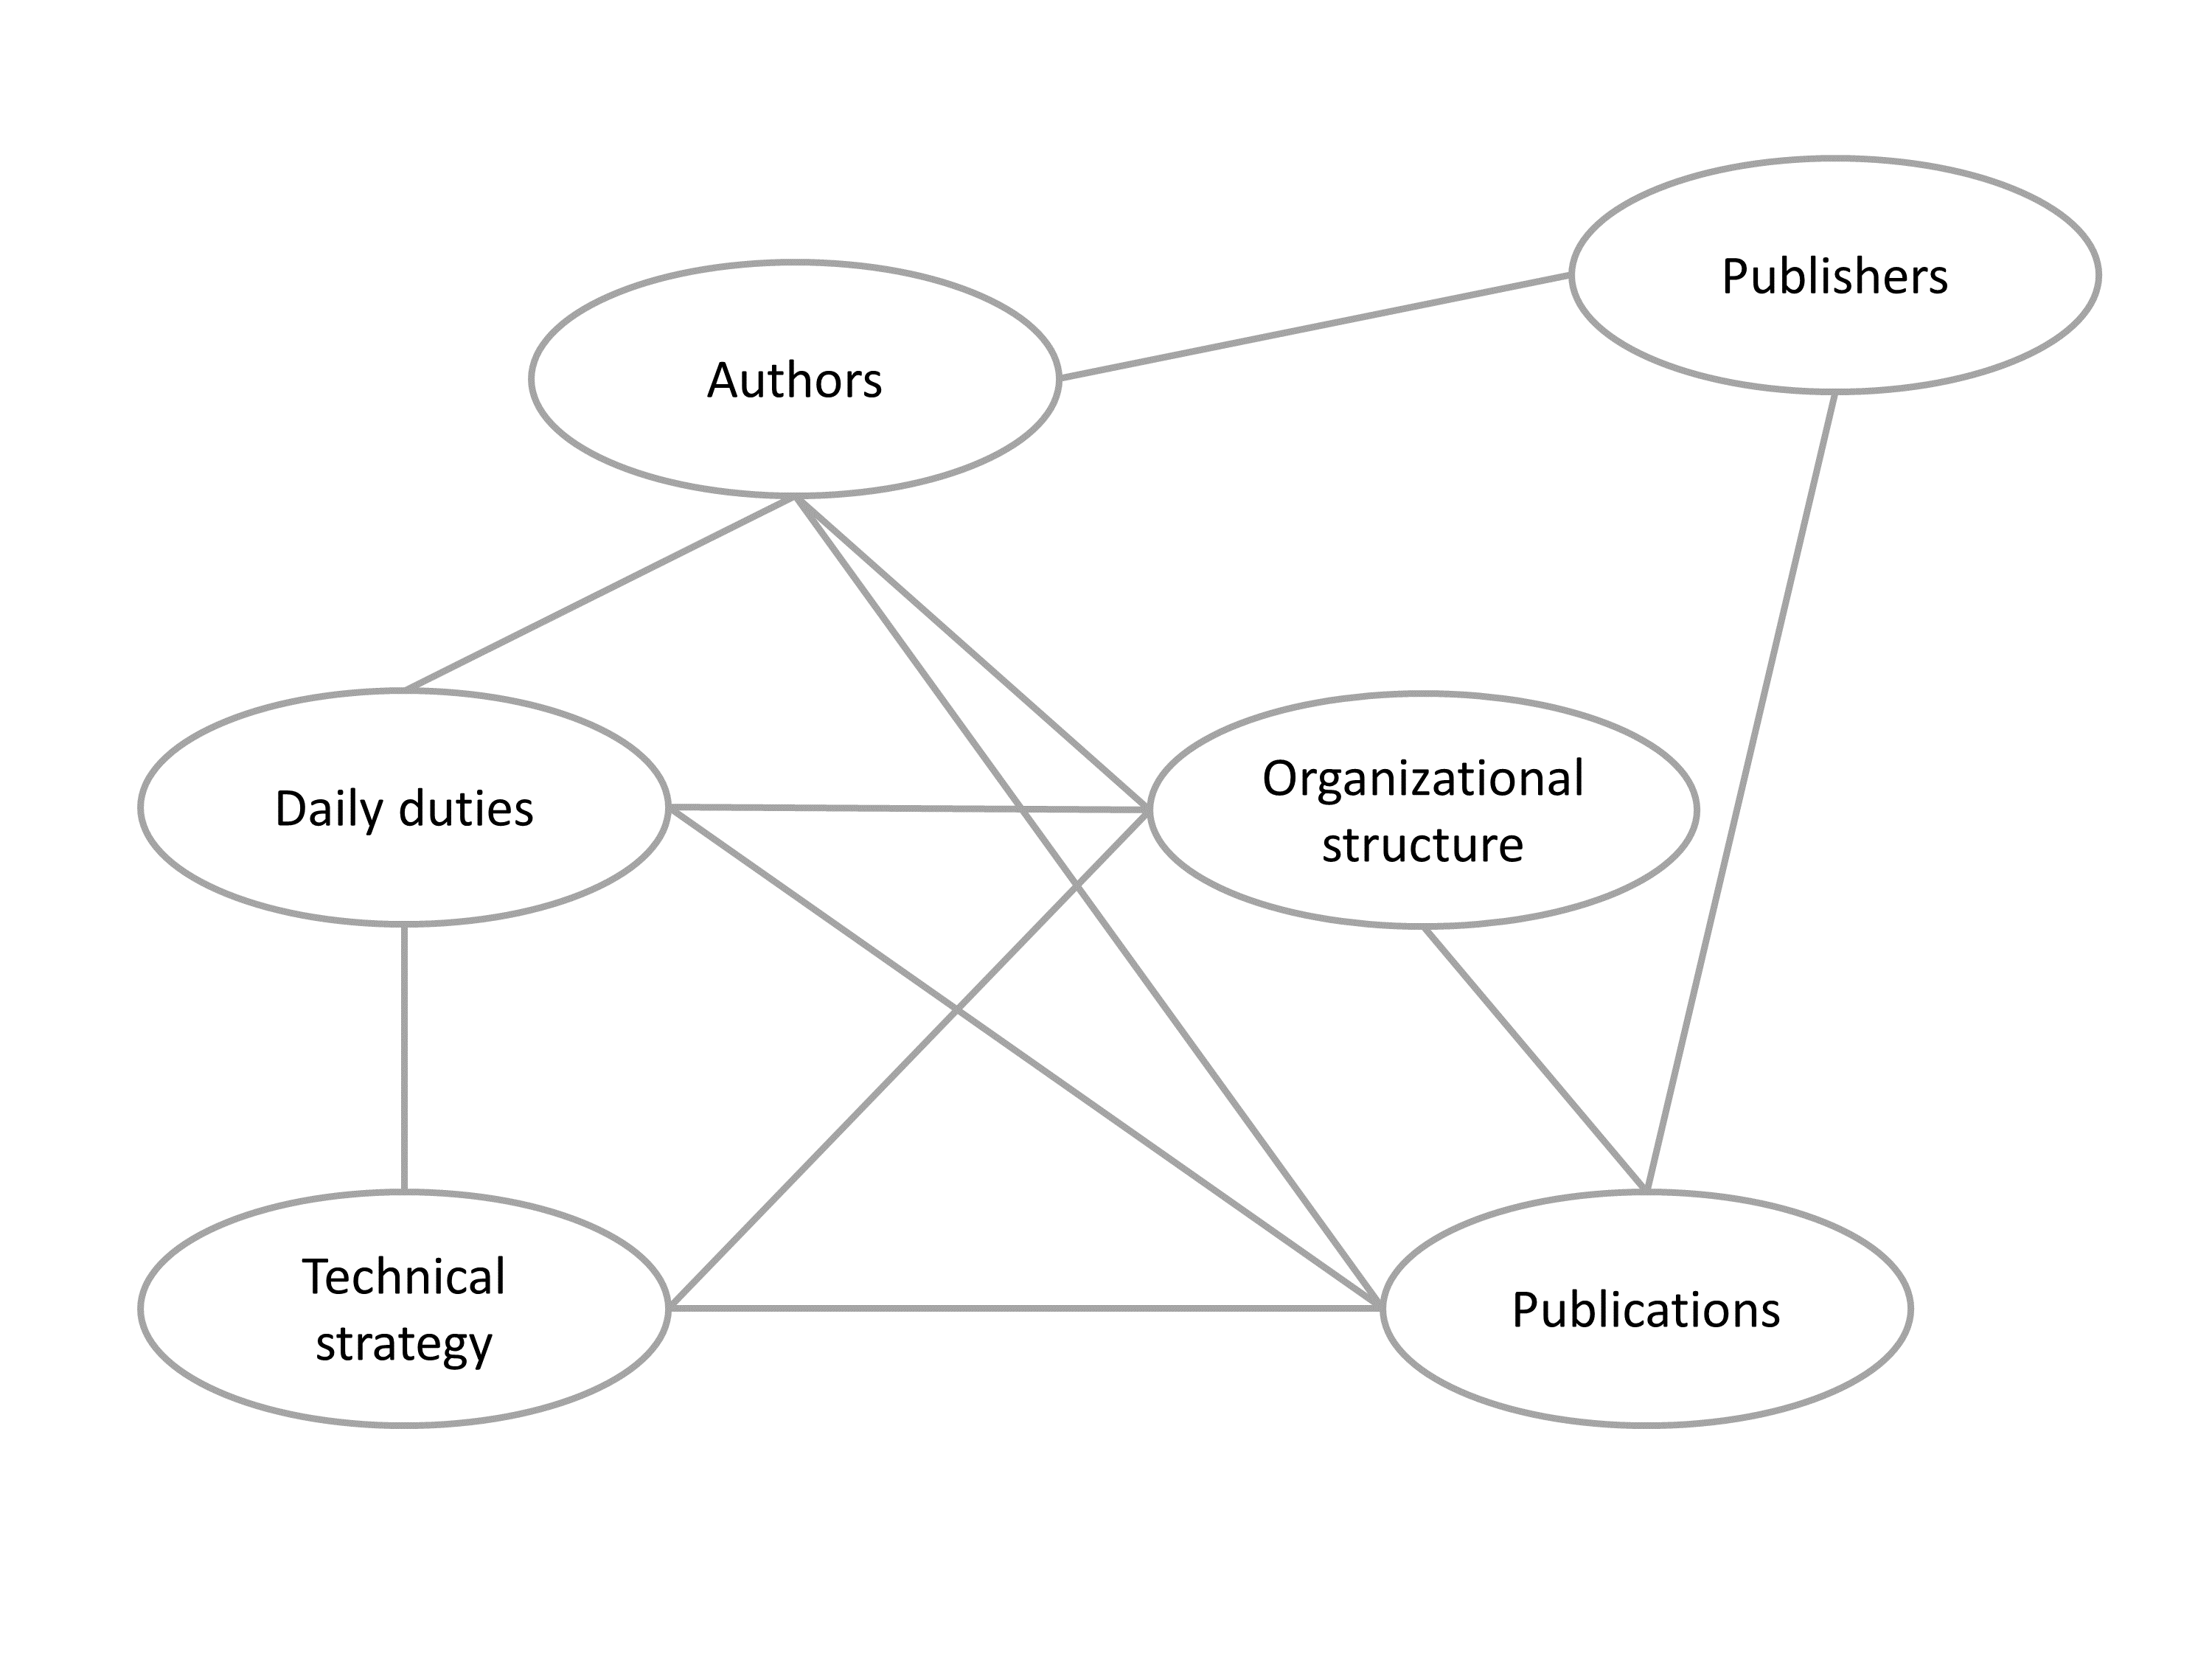
\includegraphics[width=0.99\textwidth]{bn2eng}
	\caption{The fragment of Bayesian network for STC.}
	\label{fig:bn2}
\end{figure}  

One solution may be the introduction of hidden parameters such as IC, which reduce the number of links. 
Suppose that the STC has an IC on which the number of publications and the number of authors depends. 
Thus, the number of combinations for probabilistic estimation is significantly reduced.

\subsection{The Expectation-Maximization algorithm}

Consider the probabilistic formulation of Jensen's inequality.
Let $\big(\Omega,\mathcal{F},\mathbb{P}\big)$ be a probability space, and $x\colon\Omega \to \mathbb{R}$ be a random variable defined on it. 
Let also $\varphi\colon\mathbb{R} \to \mathbb{R}$ be a convex (down) function. 
If $X, \varphi \left( X \right) \in L^1 \big(\Omega,\mathcal{F},\mathbb{P}\big)$, then $\varphi \big(\mathrm{E}[X] \big) \leqslant \mathbb{E}[\varphi (X)]$, where $\mathbb{E}[\cdot]$ means expectation. 
In other words, for the convex function $f$ and the probability distribution $t$, we obtain the following expression \ref{eq:jen}:

\begin{equation} \label{eq:jen}
f \left( \mathbb{E}_{p \left( t \right) } \, t \right) \geqslant \mathbb{E}_{p \left( t \right)} f \left( t \right)
\end{equation}

For further consideration, let us present the following definition of Kullback-Leibler divergence \ref{eq:kl0}.

\begin{equation} \label{eq:kl0}
\mathcal{KL} \left( q\vert \vert p \right)  = \int_x q \left(  x  \right)  \, \log \frac{q \left(  x \right) }{p \left(   x \right) } \, {\rm d}x
\end{equation}

Note that it is more accurate to call the Kullback–Leibler divergence an asymmetric measure of the difference between two distributions $q \left( x \right)$ and $p \left(x \right)$.
Since by definition this measure does not have symmetry \ref{eq:kl01}.

\begin{equation} \label{eq:kl01}
\mathcal{KL}  \left( q \vert \vert p \right)  \neq \mathcal{KL}  \left( p\vert \vert q \right) 
\end{equation}

Another useful property of the Kullback–Leibler divergence is shown as inequation \ref{eq:kl02}.

\begin{equation} \label{eq:kl02}
 \mathcal{KL} \left( q \vert \vert p \right) \geqslant 0
\end{equation}

To proof it let us make the following computations \ref{eq:kl03}.

\begin{eqnarray}\label{eq:kl03}
	\mathcal{KL}(q\vert \vert p) 
	& = & \mathit{E}_q \left(  - \log	 \frac{q}{p} \right) \\
	& = & \mathit{E}_q \left(  - \log	 \frac{p}{q} \right) \leqslant  \log \left( \mathit{E}_q \frac{q}{p} \right)\\
	& = & \log \int_x q \left( x \right) \, \frac{q \left( x \right)}{p \left(  x \right)} \, {\rm d}x \\
	& = & 0
\end{eqnarray}

Consider use of EM-algorithm for finding the hidden settings STC.
Assume that we have an STC model with latent parameters. 
Let's denote the latent parameters as $t_i$ and the observed parameters as $x_i$. 
Then the likelihood function can be expressed as ~\ref{eq:em0}.

\begin{equation} \label{eq:em0}
p \left( x_i \vert	\theta \right) = \sum_c p \left( x_i \vert t_i = c \right) p \left( t_i = c \vert \theta \right) 
\end{equation}

Where $p \left (t_i = c \vert \theta \right)$ is the a priori probability that $t$ takes the value $t$. 
The problem is to maximize the probability of the likelihood function by $\theta$. 
Since the logarithm is a convex continuously increasing function, we will look for the maximum logarithm of $p \left( x_i \vert \theta \right)$. 
Suppose also that all $N$ estimations of $x_i$ were made independently. 
Then the probability $X = \prod_i^N p \left( x_ \vert \theta \right) $.

\begin{equation} \label{eq:em1}
\log p \left(  X \vert	\theta \right) = \sum_i^N \log p \left( x_i \vert \theta \right) = \sum_i^N \log \sum_c p \left(  x_i \vert t_i = c \vert \theta \right)
\end{equation}

It is worth noting that we can search for the maximum expression ~\ref{eq:em1} using gradient methods. 
For example, using the stochastic gradient descent method. 
However, the author purposely used a different algorithm and showed it's advantages in the next paragraph.

Apply the Jensen inequality \ref{eq:jen} to the expression \ref{eq:em1} and get $\log p \left( x \vert \theta \right) \geqslant \mathfrak{L} \left( \theta, q \right)$.
Next, select the function $\mathfrak{L} \left( \theta, q \right)$ so that it is easy to maximize it (\ref{eq:em2}).

\begin{equation} \label{eq:em2}
\mathfrak{L} \left( \theta, q \right) = \sum_i^N \sum_c q \left( t_i = c \right) \log \frac{p \left( x_i, t_i = c \vert \theta \right)}{q \left( t_i = c \right)}
\end{equation}

So as a result, for the parameter $\theta$ and the distribution $q$ we obtain an inequality ~\ref{eq:em3}.

\begin{equation} \label{eq:em3}
\log p \left(  X \vert	\theta \right) \geqslant \mathfrak{L}\left( \theta, q \right)
\end{equation}

Now, to find the maximum of $mathfrak{L} \left( \theta, q \right)$, we apply the following two-step iterative algorithm (\ref{eq:em31}) for each iteration of $k$.

\begin{itemize}\label{eq:em31}
	\item Fix $\theta^k$ and choose $q^k$ so that $\mathfrak{L} \left( \theta^k, q^k \right)$ will maximal; 
	\item Get  $q^{k+1} = \operatorname*{arg\,max}_q \mathfrak{L} \left( \theta^k, q \right)$
\end{itemize}

The first step is called E-step, and the second M-step. 
Together, they represent an EM-algorithm whose result is $\theta$ for the hidden variable $t$.

\subsection{The E-step}

Let us consider the E-step in more detail. 
Maximizing the lower bound function $\mathfrak{L} \left( \theta^k, q^k \right)$ means that the distance between $\mathfrak{L} \left( \theta^k, q^k \right)$ and the maximum likelihood function $\log p \left( X \vert \theta^k \right)$. 
Lets write this equation for the k-th iteration (\ref{eq:em4}) and show that this distance can be expressed concerning Kullback–Leibler divergence.

\begin{eqnarray} \label{eq:em4}
	DIST & = & \log p \left( X \vert \theta \right) - mathfrak{L} \left( \theta, q \right)  \\
	& = & \sum_i^N \log p \left( x_i,\theta \right) - \sum_i^N \sum_c q(t_i = c) \log \frac{p \left( x_i,t_i=c \vert \theta \right)}{q(t_i=c)} \\
	& = & \sum_i^N  \big\{ \log p \left( x_i \vert \theta \right) \sum_c q(t_i=c) - \sum_c q(t_i = c) \log \frac{p \left( x_i,t_i=c \vert \theta \right)}{q(t_i=c)} \big\} \\
	& = & \sum_i^N \sum_c q(t_i = c) \big\{ \log p \left( x_i \vert \theta \right) - \log \frac{p \left( x_i,t_i=c \vert \theta \right)}{q(t_i=c)} \big\} \\
	& = & \sum_i^N \sum_c q(t_i = c) \big\{ \log p \left( x_i \vert \theta \right) - \log \frac{p \left( x_i,t_i=c \vert \theta \right)}{q(t_i=c)} \big\} \\
	& = & \sum_i^N \sum_c q(t_i = c) \log  \frac{p \left( x_i \vert \theta \right) q(t_i=c)}{p \left( x_i,t_i=c \vert \theta \right)}  \\
	& = & \sum_i^N \sum_c q(t_i = c) \log  \frac{p \left( x_i \vert \theta \right) q(t_i=c)}{p \left( t_i \vert x_i,\theta \right) p \left( x_i \vert \theta \right)}  \\
	& = & \sum_i^N \sum_c q(t_i = c) \log  \frac{ q(t_i=c)}{p \left( t_i \vert x_i,\theta \right) }  \\
	& = & \sum_i^N \mathcal{KL}( q(t_i) \vert \vert p \left( t_i \vert x_i, \theta \right) )\\
\end{eqnarray}

Thus, maximizing the lower bound function $\mathfrak{L} \left( \theta^k, q^k \right)$ is equivalent to minimizing the sum of Kullback–Leibler divergences for $q( t)$ and $p \left ( t \vert x, \theta \right)$. 
Since the Kullback–Leibler divergences are nonnegative by definition, we can equate them to zero to find the global minimum (\ref{eq:em5}).

\begin{equation} \label{eq:em5}
0 = \sum_i^N \mathcal{KL} \left( q \left( t_i \right) \vert \vert p \left( t_i \vert x_i, \theta \right) \right) 
\end{equation}

It is also known from the definition of the f Kullback–Leibler divergences that it is zero only if both distributions match (\ref{eq:em6}).

\begin{equation} \label{eq:em6}
q \left( t_i \right)  =  p \left( t_i \vert x_i, \theta \right) 
\end{equation}

The equation ~\ref{eq:em6} means that in order to find the optimal distribution $q \left( t \right)$ we must choose it equal to the posteriori distribution $p \left( t \vert x,\theta \right)$.

\subsection{The M-step}

At the M-step, the likelihood function ~\ref {eq:em2} is maximized at a fixed $ q \left( t \right) $ by $ \theta $.

\begin{eqnarray} \label{eq:em7}
	\mathfrak{L} \left( \theta, q \right) & = &  \sum_i^N \sum_c q \left( t_i = c \right) \log \frac{p \left( x_i, t_i = c \vert \theta \right)}{q \left( t_i = c \right)} \\
	& = &  \sum_i^N \sum_c q \left( t_i = c \right) \log p \left( x_i, t_i = c \vert \theta \right) - \sum_i^N \sum_c q \left( t_i = c \right) \log {q \left( t_i = c \right)} 
\end{eqnarray}

Note that since the expression $\sum_i^N \sum_c q(t_i = c) \log {q \left( t_i = c \right) }$ does not depend on $\theta$, it will be zeroed when differentiating. 
Thus, the expression ~\ref{eq:em7} can be transformed as follows (\ref{eq:em8}).

\begin{equation} \label{eq:em8}
\mathfrak{L} \left( \theta, q \right)  = \mathbb{E}_{q}\log p \left( X,T \vert \theta \right) + const
\end{equation}

Recall that in the expression ~\ref{eq:em8} $x$ is all data, and $T$ is all values of latent variables. 
$\mathbb{E}_{q}$ denotes the expected distribution of $q$. 
Since we choose distributions for $x$ and $T$, we can ensure that $ p \left( X,T \vert \theta  \right)$ is smooth and continuous. 
This choice will significantly simplify the finding of the extremum by $\theta$.

\subsection{Convergence of the EM-algorithm}

The EM-algorithm is designed to find the local extrema of the maximum likelihood function. 
To do this, we use the lower bound function $\mathfrak{L}(\theta^k, q^k)$, which does not decrease in the optimization process ~\ref{eq:em9}.

\begin{equation} \label{eq:em9}
\log p \left( X \vert  \theta ^{k+1} \right) \geqslant \log p \left( X \vert  \theta ^{k} \right)
\end{equation}

Use of EM-algorithm to identify hidden topics in the text.
The scientific text is one of the indications of NTC activity. 
The identification of text topics can be made using the Dirichlet distribution. 
Bayesian model for the posterior distribution of hidden topics in the text can be written in the following form (\ref{eq:lda1}).

\begin{eqnarray} \label{eq:lda1}
	p \left( W,Z,\Theta \right) = \prod_{d=1}^{D} p \left( \theta_d \right) \prod_{n=1}^{N_d} p \left( z_{dn} \vert \theta_d \right) p \left( w_{dn} \vert z_{dn} \right) \\
	p \left( \theta_d \right) \sim Dir \left( \alpha \right) \\
	p \left( z_{dn} \vert \theta_d \right) = \theta_{dz_{dn}} \\
	p \left( w_{dn} \vert z_{dn} \right) = \Phi_{z_{dn}w_{dn}} \\
	\sum_w \Phi_{tw} = 1 \\
	\Phi_{tw} \geqslant 0
\end{eqnarray}

Thus, $W$ - is text data (scientific articles, documents), $\Phi$ - word distribution in each subject, $Z$ - distribution of topics for each word, $\Theta$ - distribution of topics in the document.
The optimization task for searching for topics is as follows (\ref{eq:lda2}).

\begin{equation} \label{eq:lda2}
P \left( W \vert \Phi \right) \rightarrow max_\Phi
\end{equation}

To use the EM-algorithm, we write explicit equations for the E-step and M-step (\ref{eq:lda3}, \ref{eq:lda4}).

\textbf{E-step:}
\begin{equation}\label{eq:lda3}
\mathcal{KL} \left( q \left( \Theta \right)  \, q \left( Z \right)  \vert \vert p \left( \Theta,Z \vert W \right)  \right)  \rightarrow \underset{q \left( \Theta \right)  \, q \left( Z \right) } {\text{minimize}}
\end{equation}

\textbf{M-step:}
\begin{equation}\label{eq:lda4}
\mathbb{E}_{q \left( \Theta \right)  \, q \left( Z \right) } \log p \left( \Theta,Z,W \right)  \rightarrow \underset{\Phi}{\text{maximize}}
\end{equation}

The resulting expressions for the E-step (\ref{eq:lda3}) and M-step (\ref{eq:lda4}) allow to obtain the latent topics from text.

\section{Modeling of self-organizing teams in the scientific environment}
\label{sec:moso}

Self-organization of working groups is of great interest for scientific and technical organizations looking for new forms of practical organization of employees' work.
Consideration of the phenomenon of self-organization as an alternative to the formation of working groups led to the construction of a model of the process of self-organization.
Consideration of the life cycle of the working group concerning the goal allowed to introduce formal criteria for evaluating the effectiveness of the work of the group and predict its productivity.

An important factor affecting the productivity of the working group is the nature of the problem being solved.
The author proposed his classification of the creative tasks of the oil and gas industry from the competencies necessary to solve them.

In the framework of the developed methodology for the life cycle of the working group and the classification of tasks, a mathematical model of self-organization of working groups was built to solve creative problems. Calibration of the mathematical model of the appearance of working groups was carried out on the data of Gazprom Neft STC.

In the created system of performance indicators, a digital simulation experiment was conducted to identify the main characteristics of the self-organization of working groups.

As a result, the clustering of creative tasks on the effectiveness of solutions by various working groups was made, recommendations for creating organizational measures to increase the likelihood of self-organization of working groups were drawn up, criteria for assigning creative tasks to various types of working groups were highlighted, the main criteria for forming active working groups were identified.

Modeling group actions of individuals depend on potential participants in the group and goals.
For example, fans of a football club can easily be combined into a group, but they do not have a specific goal.
On the other hand, scientists can join a research group for a specific purpose, for example, writing a scientific article.
Are the joining principles the same in these cases?

There are two ways  of the appearance of groups:
\begin{enumerate}
	\item Self-organization - the process of organizing employees due to internal factors, without external specific impact, 
	\item Formation and promotion of members of the group from the outside.
\end{enumerate}

Example of forming a group in an organizational environment: 

\textit{The head of the Department decides to form a working group to create an oilfield improvement system of two field developers. }

An example of self-organization of groups in an organizational environment: 

\textit{Several field developers have decided that together they need to improve the methods of processing data on the unique modes of operation of wells using machine learning algorithms and selflessly work together on the weekends on this task.
}\label{exp:2}

The decision to create a group inside leads to self-organization, the decision to create a group from outside forms a group.
Note that in practice the process of the emergence of working groups is a superposition of self-organization and formation.
However, for research purposes in this paper, the authors intend to consider the formation and self-organization separately to identify the common characteristics of these phenomena.

A group is created for a specific time and a specific task.
In this sense, the signs of the project activity are evident - the uniqueness of the result and the limited resources to achieve the goal.
Thus, it seems reasonable to apply the project methodology for assessing the effectiveness of the group as a project team.

The group structure is determined by the nature of the tasks to be solved.
For tasks of mass service, for example, in working groups in call centers unite specialists with a precise, identical profile of competences.
There is almost no separation of duties in such a group: typical maintenance tasks require standardized actions by group members.
The workload is evenly distributed across the group members.

The group created to solve the creative problem is not homogeneous.
Specialists with different competencies are needed to solve the creative problem.
Figuratively, we can imagine how the task is decomposed into the competence of the participants.
Moreover, this is not a uniform distribution. 
The participants get different amounts of work within their competencies.
For the above example (\ref{exp:2}), the task requires competences in the technical modes of operation of wells and methods of machine learning.
What will happen if the competencies needed to achieve the goal are needed more than the group has?
Each of the group members will perform work within their competencies, but the goal will not be achieved, as there will be outstanding work.
This circumstance is a common situation, as with the wrong planning of groups (formation), and with self-organizing groups.
The result of work in such a situation turns out to be negative, but the attitude to this result is different in the case of self-organization and formation.

The main criteria for the effectiveness of the working groups are the result of their activities and the timing for achieving this result - these are generally accepted organizational performance indicators.
The study of the phenomenon of self-organization of working groups in the dynamics is a complex organizational task.
Therefore, the author used in this work a mathematical model of the phenomenon of self-organization of working groups.
The mathematical model makes it possible to study the most characteristic aspects of the phenomenon of self-organization, but it has a certain degree of approximation, inaccuracy.

A computational experiment by the created model of self-organization of working groups, which is presented below, evaluatштп the results of the work of various groups on various tasks.
In connection with this formulation of the experiment, the following research questions arise: 

In connection with this formulation of the experiment, the following research questions arise:

\begin{enumerate}
\item 
How do groups self-organize? 
Which employees can self-organize and which ones not? 
How does self-organization is influenced by competences, experience, social factors?
\item 
What organizational conditions are necessary for the self-organization of groups in a scientific and technical environment? 
\item 
What type of tasks do self-organized groups cope with more efficiently than formed ones?
\item 
What are the principles of forming groups for the most effective solution to creative problems?
\end{enumerate}

Numerous publications are devoted to the evaluation of the effectiveness of research and development projects, as well as to the study of factors affecting the effectiveness of scientific activities, see, for example, \cite{shcherb1982, ovch2009,fursov2016,shmatko2017}.
As a rule, in these works the research team is considered as a ``black box'', producing scientific results, and evaluation of its effectiveness is made only by the results, the internal structure of the research team is usually not taken into account. 
Self-organizing teams are studied in detail in \cite{moe2008understanding}.  
Separately examines the motivating factors \cite{shmatko2017} and the factors influencing the performance of \cite{fursov2016}.

At the same time, the topic of modeling and analysis of teamwork is also well developed and actively studied since the middle of the XX century, see \cite{bavelas1948mathematical,nov2008, bei2014}. 
A formal description of the competence profile is the subject of numerous studies and publications, see, for example, \cite{rozewski2009competence,bei2014}.

The first approximation may be a model limited to the existence of a fixed set of specific skills. 
In this case, the competence profile of each employee can be described as a vector of values, in which each coordinate describes the level of his knowledge of the relevant skill.

The vector describing the competence profile of the team is the result of the simple addition of the competence profiles of the participants. 
Such a model naturally occurs if we measure the level of competence by performance when performing the appropriate type of tasks. 
Then it is natural to assume that when working together in a team, the performance of the participants develops.

A similar vector can also describe the profile of the problem.
A certain level of performance is required for each type of task in order to prepare and conduct a scientific study, taking into account the time limit.

In this study, the author consider small self-organizing teams, in which the initiative of creation comes from employees. 
This assumption corresponds to the real situation in most research teams, where the administration can motivate employees in various ways to apply for participation in a scientific conference or recommend to prepare an article for a particular journal, but the final decision, as a rule, remains for the researcher.

In this study, it is assumed that the list of competencies and the level of experience are the criteria from which the employee decides to join the team.

A set of topics that correspond to the sequence of incoming invitations from conferences and journals to which applications are open is considered as input to the model. 
One or more topics are known for each event or publication. 
Preparation of an article on a given topic requires a specific set of competencies. 

The space of scientific activity determines competencies. In the oilfield services industry, the set of competencies differs from the set of competencies in the wood processing industry. 

Experience describes a vector of a certain length and direction in the competence space. 
The projection of the vector on the axis experience competencies demonstrate experience in or the necessary skills. 

A task, for example, the topic of a scientific article, also represents a vector in the space of competences. 
Topics may require competencies that authors do not possess individually. 
Each co-author closes only a part of the competencies required for solving the problem (writing the article).

\subsection{Starting the team building process}

The process of formation of the team starts with taking the first participant of the decision on the establishment of the team for the preparation of an application for a conference or article in the collection.
Usually, this happens as follows. 
An unoccupied employee reviews the list of invitations and evaluates his / her competencies regarding the announced topics. 
If at least one of his competencies meets or exceeds the requirements of the goal, he decides to create a team and becomes its first participant.
At the initial moment, the competence profile of the team coincides with the profile of the first participant.
The following participants will join this team taking into account the requirements corresponding to the chosen topic, as well as the competence profiles of other team members.

\subsection{Joining new members to the team}

The second (subsequent) participant will learn from one of the team members about the purpose and assessment of the current competencies of the team. 
This information is shared between staff members who are quite familiar with each other. 
In the model, this is represented by a communication graph. 
Each participant evaluates his competences for the needs of the team to achieve the goal and make a decision about joining the team. 
The solution is positive if at least one of the competencies of this participant when adding to the profile of the team brings it closer to the goal.

\subsection{Finalizing the team}

Because of the limited time to solve the problem, the time to form teams cannot be unlimited.
If during the allotted period the team with the required set of competencies could not be formed, the process stops, the participants are released from their obligations and switch to the search for another task. 
If the team is successfully formed, we believe that its members are busy for some time and the result of this work is the publication.

\subsection{Formal competency model}

Let $N$ denote the number of key skills required to work in a given subject area, $W$ denotes the number of employees in an organization. 
Then the competence profile for the employee is called vector $\vec{\kappa} \left (w \right)$ (\ref{eq:team1}).

\begin{equation}\label{eq:team1}
\vec{\kappa}\left( w \right) = \left( \kappa_1, \ldots, \kappa_{\bf N} \right) \mbox{, where } w \in {W}, \kappa_i \in \mathbf{R}^{+}
\end{equation}

The competence profile of a team $T$ consisting of $M$ a person is a vector of the same dimension $N$, which is defined as the sum of all team members (\ref{eq:team2}).

\begin{equation}\label{eq:team2}
\vec{\kappa} \left( T \right)  = \sum_{i=1}^{{\bf M}}
\vec{\kappa} \left( w_i \right) \mbox{, where } T= \{w_1, \ldots, w_{\bf M} : w_i \in {W} \}
\end{equation}

Informally, the $i$-th component of the vector corresponds to the performance of a person and a team when performing tasks of a particular type.
The theme profile $p$ has the same type. Namely, it is an $N$ - dimensional vector \ref{eq:team3}.

\begin{equation}\label{eq:team3}
\vec{\kappa} \left( p \right) = \left( \kappa_1, \ldots, \kappa_N \right)
\end{equation}

In equation  \ref{eq:team3}  $i$-th component of the vector corresponds to the minimum performance of the team, in which all tasks of the corresponding type will be performed on time and with proper quality.

\subsection{Key decision making model}

The key functions are those that simulate the logic of decision-making at different stages of team formation implementing the process of team erection:
\begin{itemize}
	\item
	$\alpha(w, p) $ describes the goal selection by the first team member, namely $\alpha(w, p)=1$ if the employee $w$ considering the goal $p$ makes a positive decision about team creation and $\alpha(w, p)=0$ otherwise; 
	\item 
	$\beta (w, T, p)$ formalizes the decision to join the team by the second and subsequent participants;
	\item 
	$\gamma (T, p, t)$ models self-timer solutions at time t based on the comparison of the created team profile and the task profile. 
\end{itemize}

This study assumes that $\alpha$, $\beta$, and $\gamma$ are deterministic Boolean functions that depend only on the competence profile of the individual, team, and task, respectively:

\begin{eqnarray} \label{eq:team4}
	\alpha(w, p) = \alpha'(\vec{\kappa}(w), \vec{\kappa}(p)),\\
	\beta(w, T, p) = \beta'(\vec{\kappa}(w), \vec{\kappa}(T), \vec{\kappa}(p)),\\
	\gamma(T, p, t) = \gamma'(\vec{\kappa}(T), \vec{\kappa}(p), t).
\end{eqnarray}

Let $\bf K$ denote the whole space of possible values of the competence vector. 
Then the fact that in our model the algorithm of team building depends only on the participant's competence profiles, team and goal set the type of functions $\alpha'$, $\beta'$ and $\gamma'$:

\begin{eqnarray} \label{eq:team5}
\alpha': {\bf K} ^2 \to \{0, 1\},\;\;\;
\beta': {\bf K} ^3 \to \{0, 1\},\;\;\;
\gamma': {\bf K} ^2 \to \{0, 1\}
\end{eqnarray}

These functions can be described as the following logical formulas:

\begin{eqnarray} \label{eq:team6}
\alpha'(x,y)=1 \iff \exists i (x_i \geq y_i) \\
\beta'(x,y,z)=1 \iff \exists i [(x_i > y_i) \wedge (y_i < z_i)]  \\
\gamma'(x,y,t)=1 \iff \exists i (x_i < y_i)  \wedge (t > \tau_{\max})
\end{eqnarray}

\subsection{Team building process}

At the time of team building, the list of open problems ${P}$ is fixed, and for each specific problem, $p\in {P}$ its profile $\kappa(p)$ is set. 
Also fixed set of employees $W$ and for each employee, $w\in W$ the profile of his competences $\kappa(w)$is known. 
Also, the graph of communications between employees $G\subseteq W\times W$ is given. 
Another parameter is the time $\tau_{\max}$ during which the team should be generated.

At each step, the following occurs sequentially.

\begin{enumerate}
	\item 
	Each employee $w_0$ who is not included in any of the teams and has not received an invitation to join the team considers the list of goals $P$. 
	If there is $p_0$ for which $\alpha (w_0,p_0)=1$, the employee decides to create a new $T_0$  team and sends invitations to join the team to all neighbors in the communication graph $G$.
	\item 
	If the co-worker $w_1$ was not included in the  team and received an invitation to enter the $T_1$  team created to solve the $p_1$ problem, he accepts the invitation if $\beta(w_1, T_1, p_1) = 1$ and sends invitations to all his neighbors in the $G$column. 
	Otherwise, the invitation is declined.
	\item 
	If the $\gamma(T_2, p_2)=1$ condition is met for some $T_2$  team created to solve the $p_2$ problem, the  team starts and all prompts are canceled.
	\item 
	If for some team $T_3$, created to solve the problem $p_3$, after a specified time $\tau_{\max}$ condition $\gamma(T_3,p_3)=0$, this  team is disbanded and all invitations are canceled.
\end{enumerate}

Even though $\alpha$, $\beta$ and $\gamma$ are deterministic, the algorithm admits a large degree of uncertainty, which is associated with the non-deterministic nature of the interaction of objects within the system. 
In particular, the result is significantly affected by the following parameters, which are implemented probabilistically:
\begin{itemize}
	\item the order of consideration of the task list by a free employee:
	\item the order of the consideration the employee received invitations;
	\item the order in which employees are selected to apply the next step of the algorithm. 
\end{itemize}

The constructed model is the basis for further research of the process of formation and functioning of project teams in the scientific environment. 
In particular, on its basis, it is planned to develop a methodology for assessing the effectiveness of research activities.
Also interesting is the refinement and expansion of the model, in particular:

\begin{itemize}
	\item 
	Competency models can be refined using fuzzy logic.
	\item 
	When modeling long-term periods, there is a need to take into account the professional and career development of employees and the associated changes in their competence profiles. 
	\item 
	Functions $\alpha$, $\beta$ and $\gamma$, describing the process of making key decisions, can be refined by taking into account other individual and team characteristics, as well as the specifics of the tasks.
	\item 
	The team building algorithm can have a more complex iterative logic that takes into account different approaches to flexible project management.
	\item 
	A separate study deserves the situation with the unsuccessful completion of the project. 
	Regarding scientific activity, this means that the written publication has not been accepted for publication, but the results are a good start for further work. 
	In the current work, the author made the assumption that employees do not write \textit{into the desk}, and each co-authorship leads to publication.
\end{itemize}

\section{Methodology of the co-authorship graph}
\label{sec:coat}
The current practice of constructing graphs of co-authorship involves the use of the mathematical apparatus of graph theory. 
Traditionally, undirected graphs are used to construct co-authorship graphs.
The co-authorship graph provides a visual visualization of the chosen scientific community and allows analysis using such common graph metrics as: Betweenness centrality \cite{leifeld2017collaboration, koseoglu2018authorship,ho2017basic} and Closeness centrality \cite{chang2017hidden,paraschiv2017semantic,ahmed2017analysis}. 
These metrics, as well as the Degree metric, are intended for formal selection of important vertices of the graph.

\subsection{Bipartite graphs}
\label{sec:coath}
An essential aspect for the construction of the graph of co-authors is the selection of data for analysis. 
Usually, researchers use public bibliographic information containing a list of co-authors. 
The source of such information may be Google Scholar, ArXiv and other online libraries. 
The consideration of open scientific communities is as interesting as the narrowing of the sample to one country \cite{krasnov2013measurement}, industry \cite{gielfi2017university} and even organization \cite{kradoya2016structure}.
Adding fields related to the author's affiliation into the graph allows us to research the relationship of organizations.
As an example, in \cite{gielfi2017university} the authors analyze the links between research institutes and industrial research centers in the oil and gas industry.
This approach to sampling allows us to analyze the topology of relationships between organizations, based on the authors ' affiliation with the organization. 

Note that all the above studies do not take into account the content of research articles.
This feature will be important in the future. 
The average number of co-authors may vary depending on the industry, but overall the number of co-authors is growing.
We note this fact as a structural feature of the study area. 

In the above study, the co-authorship graph is built on an undirected graph.
The authors are equivalent in co-authorship, although it is not. 
In the work of the author \cite{krasnov2017model} the structure of the team of co-authors is analyzed, and possible roles in the research process are formulated. 

Besides, in the traditional construction of the graph of co-authorship, information on all joint research work is contained in the edges of the graph. 
Often edges are drawn with different thickness or color depending on the number of collaborations, but this characteristic of edges is not considered in the context of graph metrics, as it does not reflect the communication meaning of re-authorship.
Taking into account these limitations, we formulate the following research questions:

\begin{itemize}
	\item Are there other ways to construct a co-authorship graph? 
	\item What are the advantages and disadvantages of different ways to build a graph of co-authors? 
	\item What are the quantitative, comparable characteristics of co-authorship graphs?
\end{itemize}

In the above studies, the graph of co-authorship is constructed as an undirected graph: articles become equivalent edges connecting authors.
The author of this study believes that the construction of the co-authorship graph as a bipartite graph will be more informative.
Such an approach makes it possible to include information on scientific articles in the co-authorship graph.
The Figure \ref{fig:bi1} shows the basic principle for constructing a graph of co-authors by a directed bipartite graph.

\begin{figure}[ht]
	\centering
	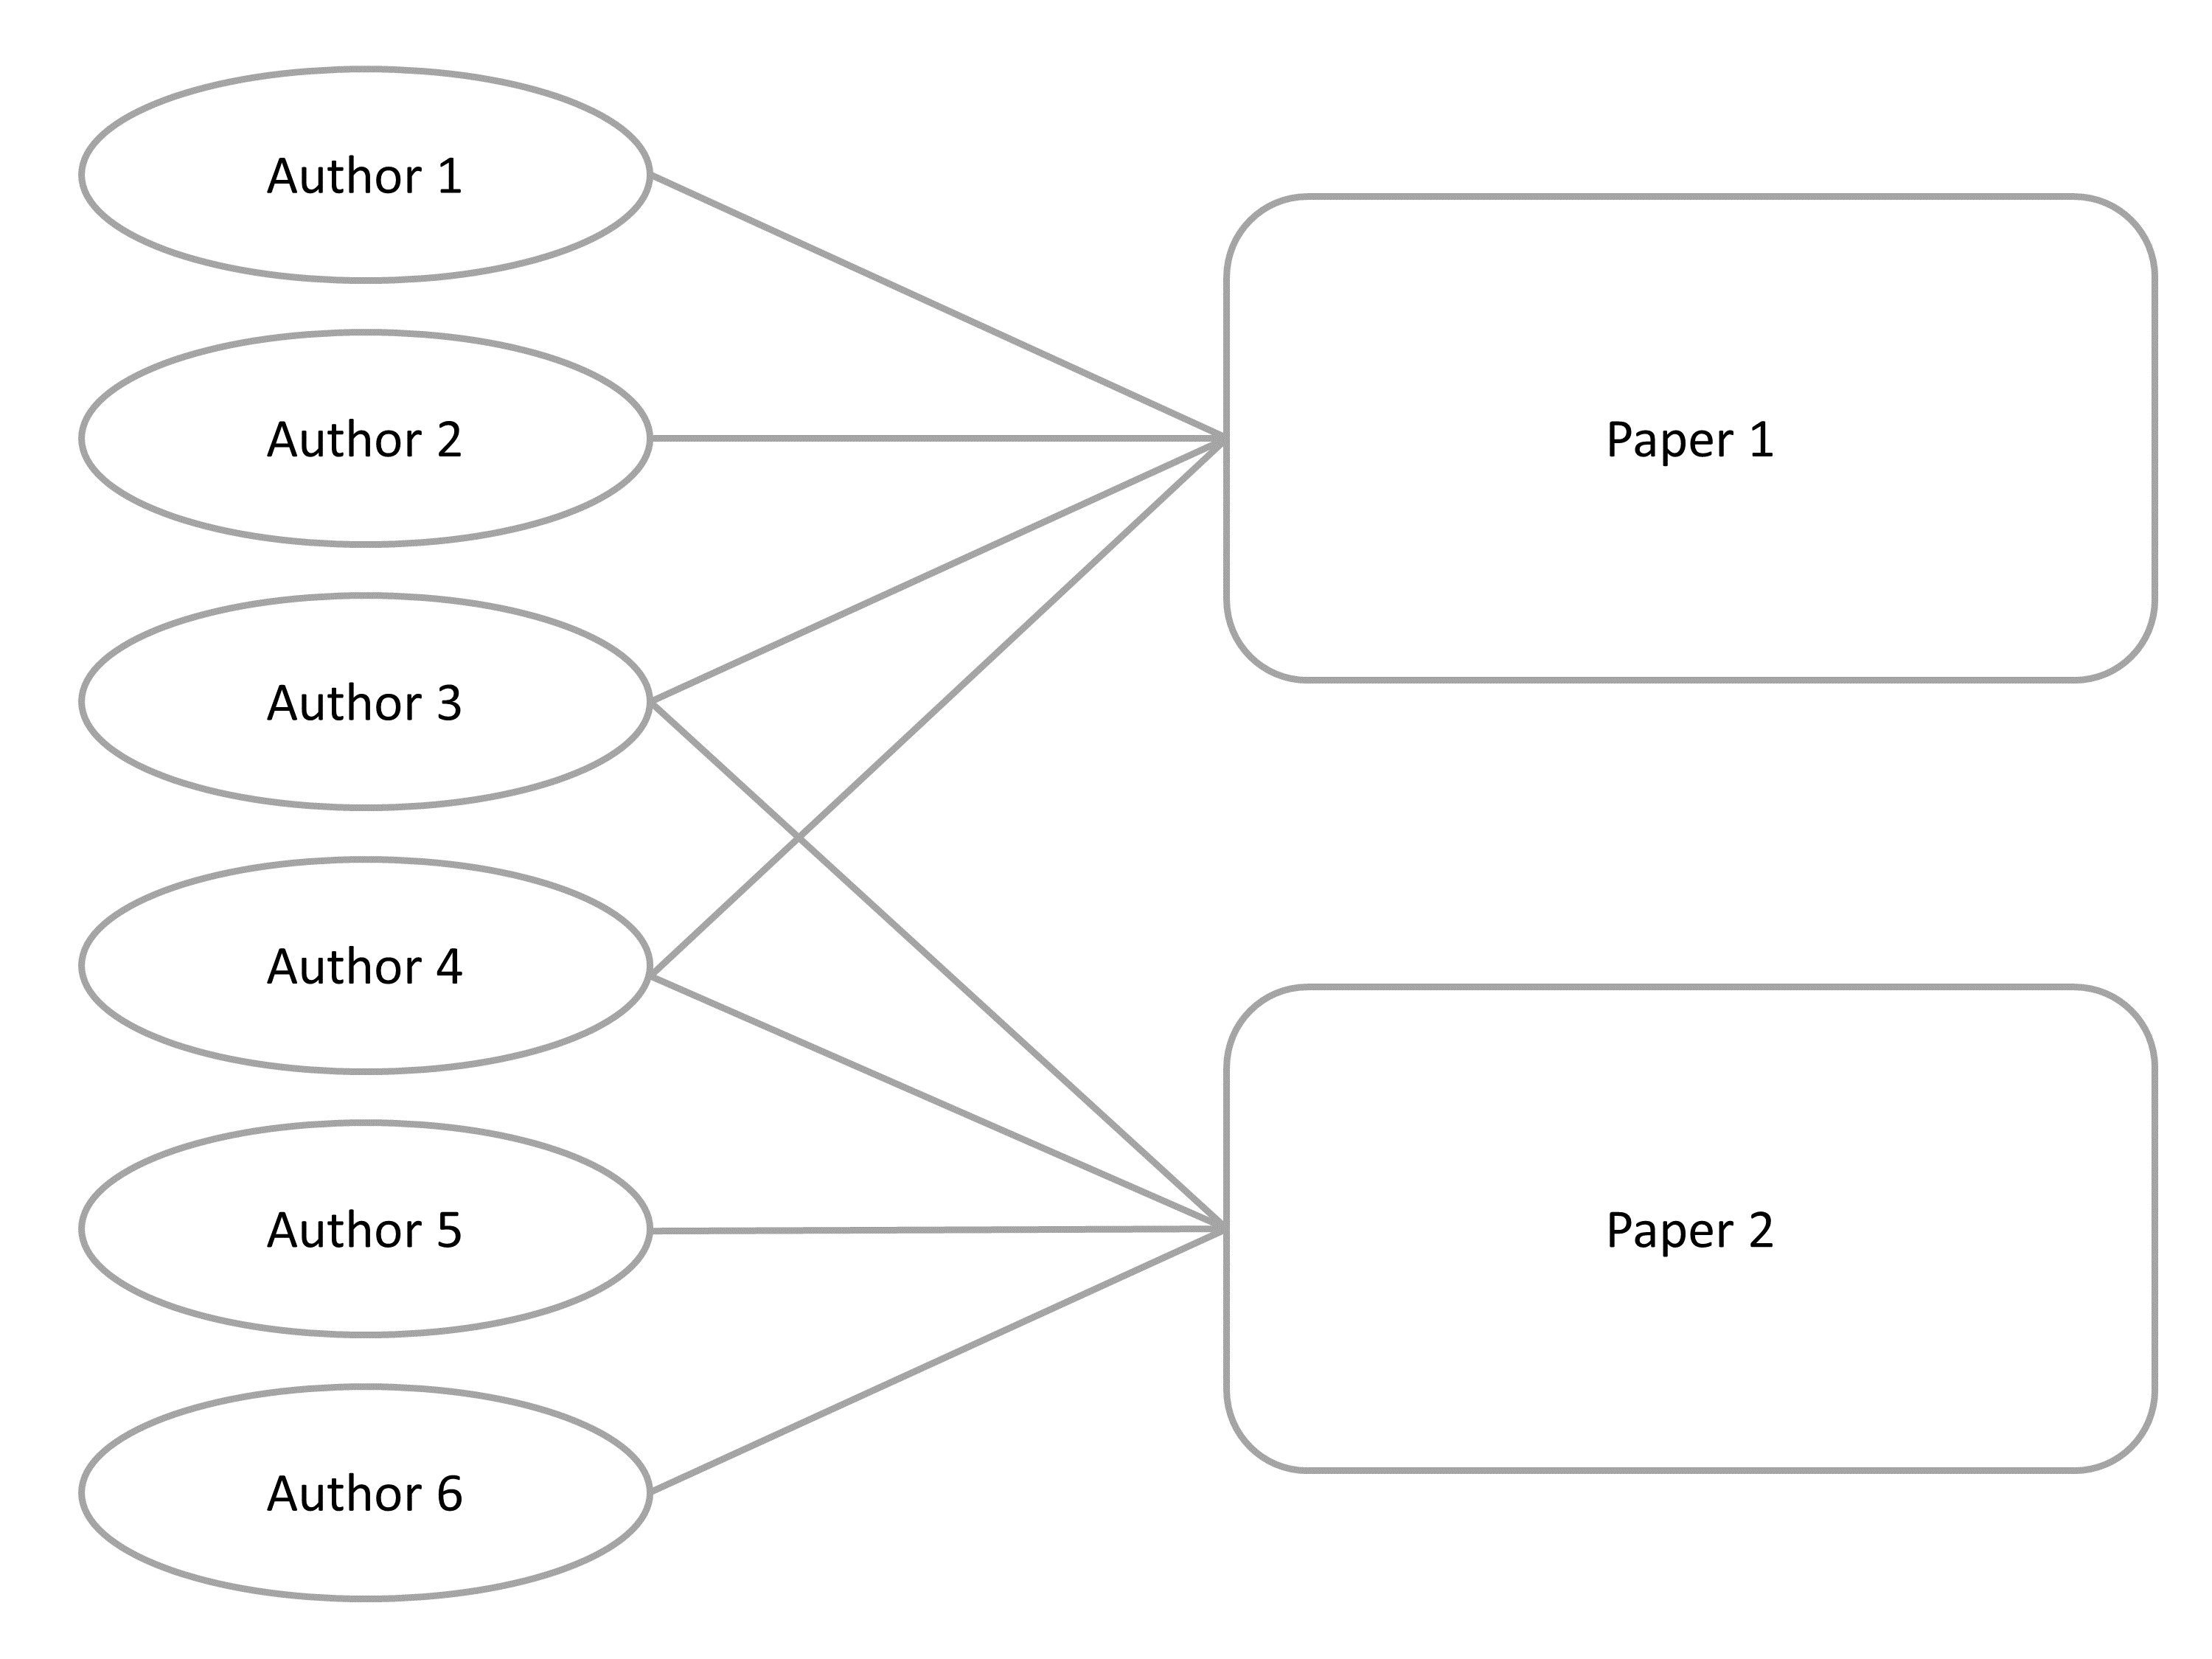
\includegraphics[width=0.8\textwidth]{bi1eng}
	\caption{Bipartite graph of co-authorship.}
	\label{fig:bi1}
\end{figure}  

The advantages of this approach are that in the graph of co-authors it becomes possible to save for further analysis the bibliographic information about the article: 

\begin{enumerate}
	\tightlist
	\item the title of the article 
	\item publication year 
	\item the publisher 
	\item keywords 
\end{enumerate}

Note that the traditional representation of a co-authorship graph as an undirected graph is a projection of a bipartite graph onto the set of vertices of the authors. 
Let us explain this in more detail. 
An oriented graph $G = (V,E)$ is called bipartite if the set of its vertices can be divided into two parts $ a \cup P = V$, such that 
\begin{itemize}
	\item no vertex in $a$ is connected to vertices in $P$
	\item no vertex in $P$ is connected to vertices in $a$.     
\end{itemize}

In this case, $A$ is a set of authors, $P$ is a set of articles. $A$ and $P$ are parts of the graph $G$.
Note that the graph $G$ can be either complete or incomplete depending on whether the authors have connections to all the articles. 
Shown in Figure \ref{fig:bi1} bipartite graph is incomplete. 
Let's denote $G_A$ projection of the graph $G$ on the set of vertices $a$.
The graph $G_A$ is a traditional representation of the graph of co-authors and is shown in figure \ref{fig:bi2}.

\begin{figure}[ht]
	\centering
	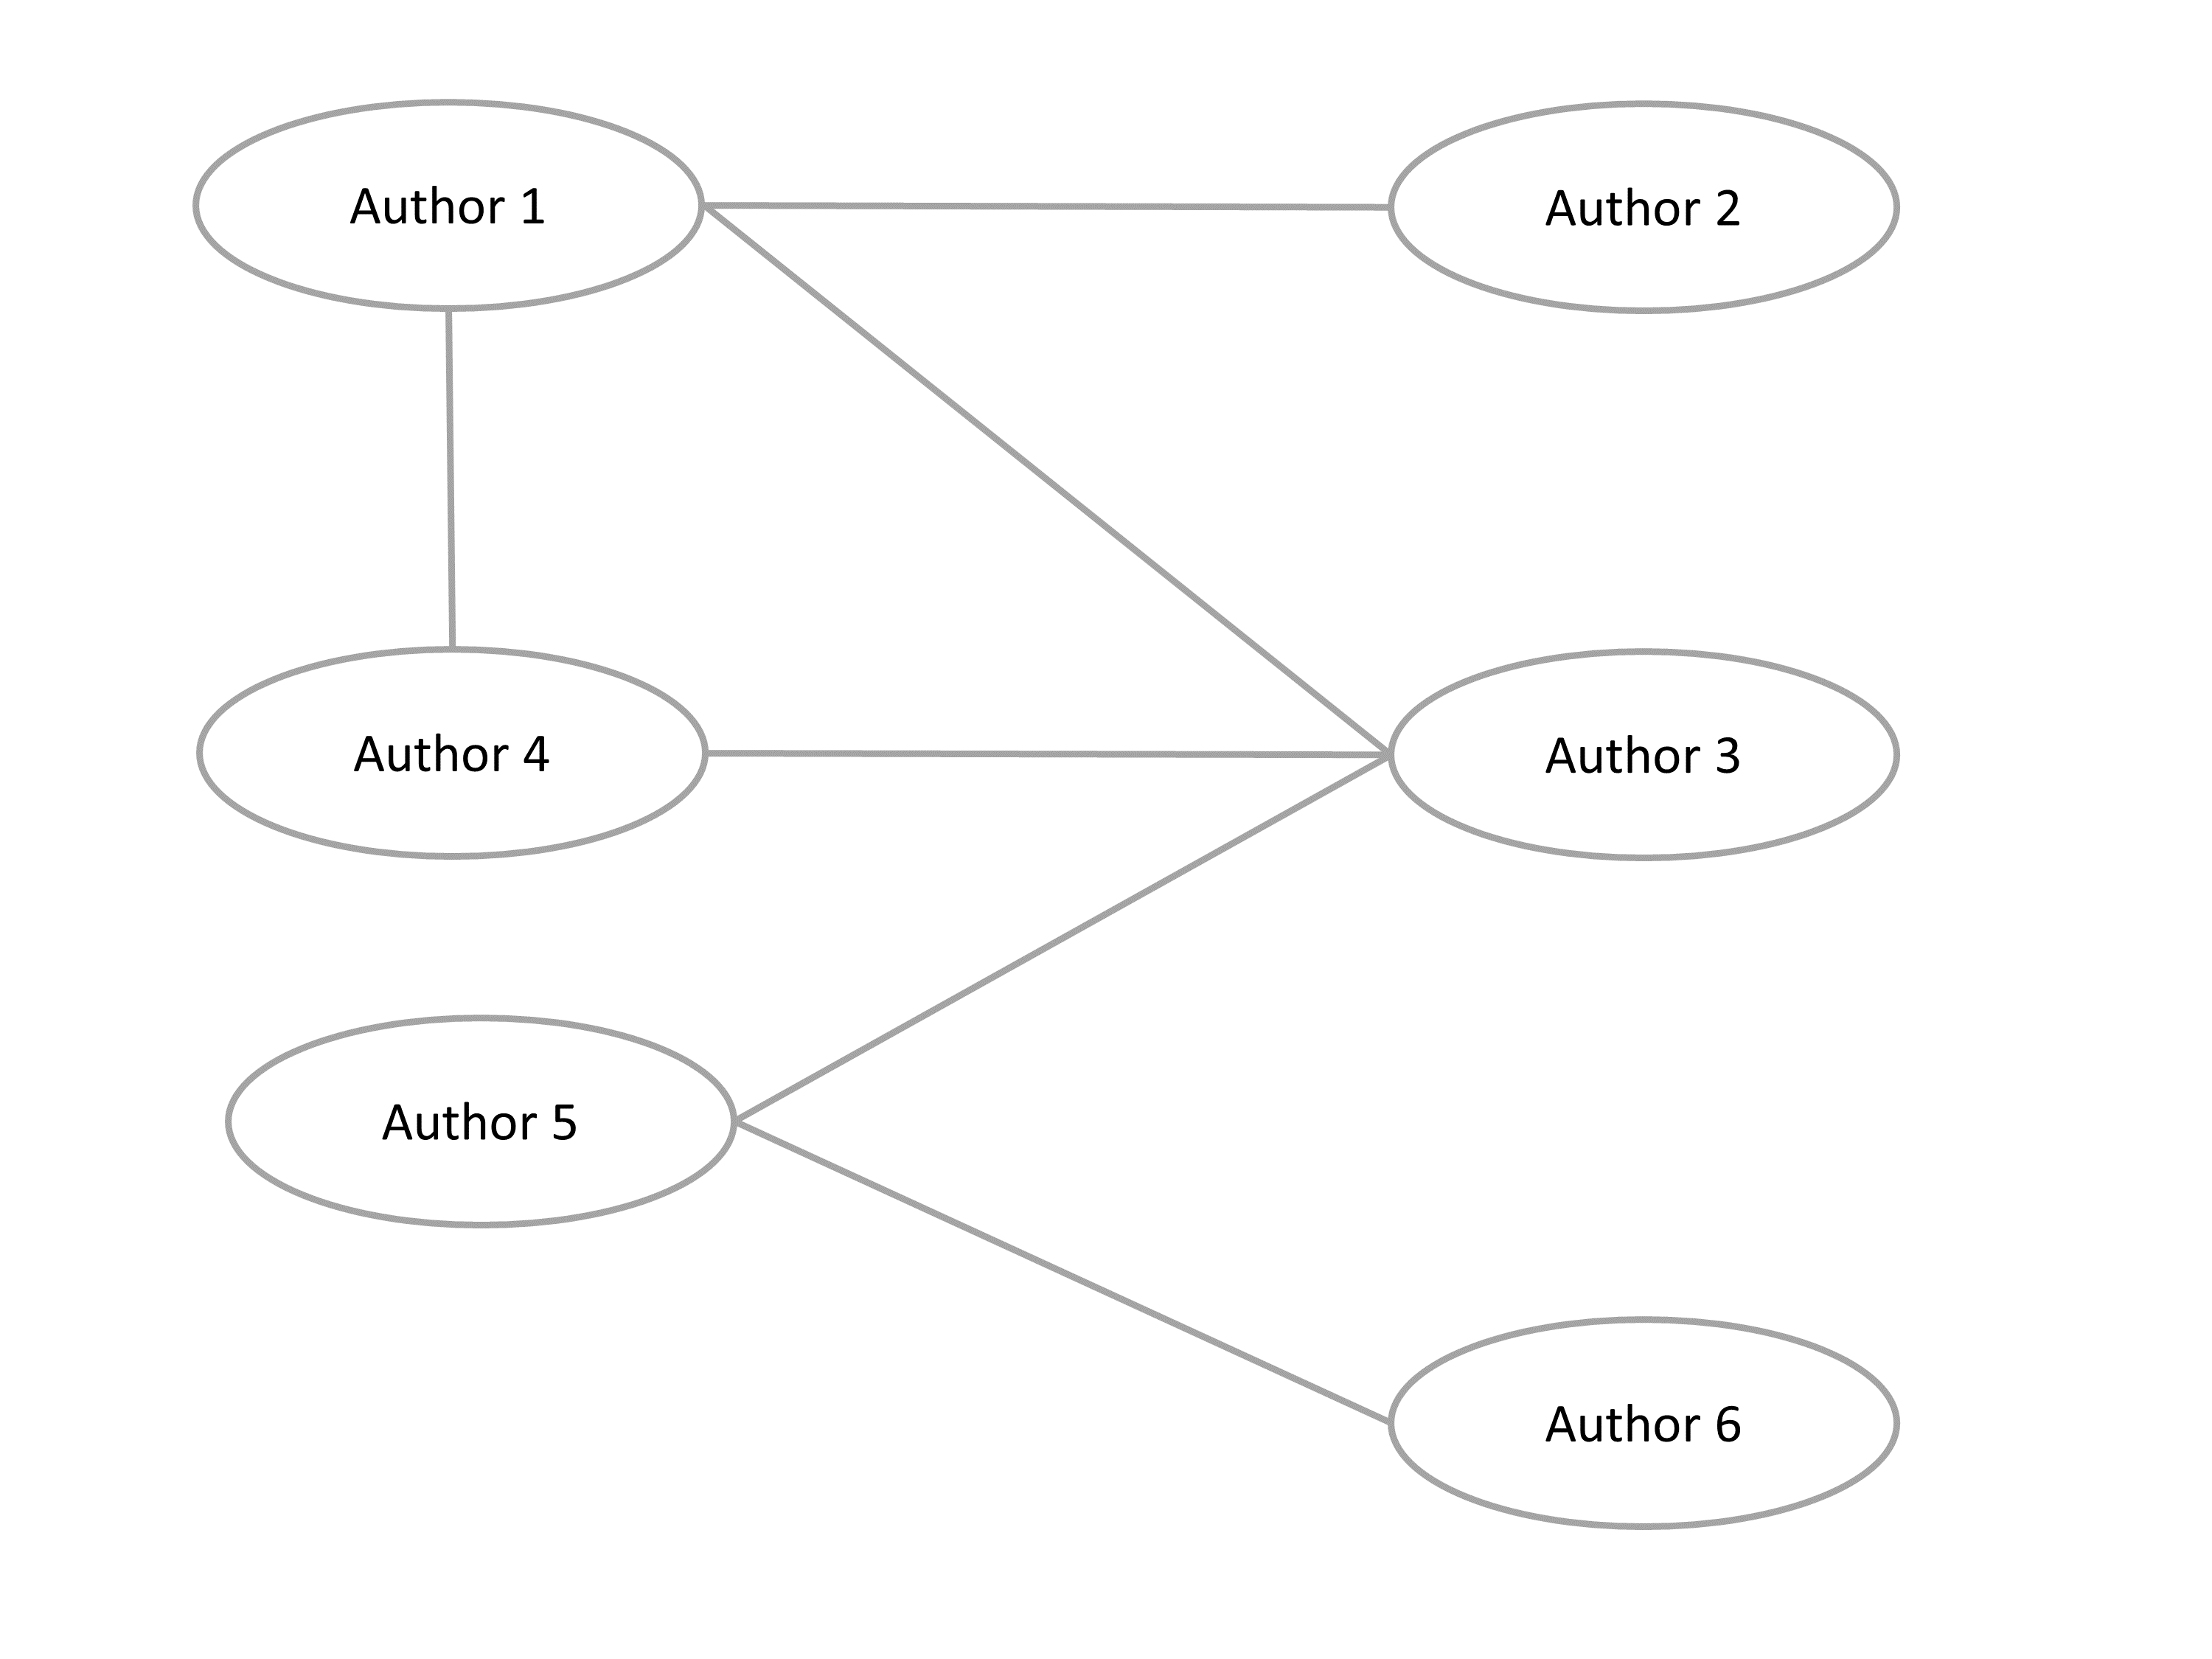
\includegraphics[width=0.8\textwidth]{bi2eng}
	\caption{Undirected co-authorship graph.}
	\label{fig:bi2}
\end{figure}  

From the figure \ref{fig:bi2} we can see that when constructing the projection, only cumulative characteristics of co-authorship can become the attributes of edges of the graph $G_A$.
For example, the number of co-authorships of two authors.

\subsection{Modeling of the co-authorship graphs}
The following stochastic approaches are widely used to model co-authorship graphs as a social network: 
\begin{enumerate}
	\item Random graphs,
	\item Small-world model,
	\item Preferential attachment model.
\end{enumerate}

One of the essential limitations of stochastic models is the fixed number of vertices and their constant growth. 
In practice, the number of potential co-authors changes in the organization.
It is also important to understand that stochastic models aim to model a graph with specific parameters. 
Such as clustering and density.

On the other hand, the formation of small groups, which include a group of co-authors of the scientific article, is modeled by the principle of additional competencies related to the class of deterministic methods of creating graphs of co-authorship. 

A combined machine learning-based approach is used to predict new vertices of the co-authorship graph. 
There are a preliminary selection of the authors' features, statistical indicators of activity for the last few time intervals, as well as structural indices of influence and local metrics in the co-authorship network. 
The results obtained in this study allow the author to conclude the applicability of communication prediction methods for the analysis of collaborative behavior patterns in a large organization with a dynamic team structure, as well as changing external and internal factors affecting individual and collective publication activity.

The basis for predicting changes in the graph of co-authors for the scientific and technical center are the following components: 
\begin{itemize}
	\item Current structure of the co-authorship graph,
	\item External impacts,
	\item Internal changes. 
\end{itemize}

Consider each of the components in more detail. 
The current structure of the co-authorship graph represents a set of metrics describing a given co-authorship graph.
These metrics include the following:

\begin{itemize}
	\item For the edges
	\begin{itemize}
		\item Common Neighbours (CN)
		\item Salton Index (SI)
		\item Jaccard Index (JI)
		\item Hub Promoted Index (HPI)
		\item Hub Depressed Index (HDI)
		\item Leicht-Holme-Newman Index (LHN1)
		\item Preferential Attachment Index (PA)
		\item Adamic-Adar Index (AA)
		\item Resource Allocation Index (RA)
	\end{itemize}
	\item For the vertices 
	\begin{itemize}
		\item Degree centrality
		\item Betweenness centrality
		\item Closeness centrality
		\item Harmonic centrality
		\item Clustering
	\end{itemize}
\end{itemize}

Each of these metrics represents a specific set of features of the co-authorship graph, affecting the forecast of its changes.
External influences to the scientific and technical center compose of the publication policy of editorial offices publishing scientific articles.
In the simplest case, the lack of opportunity to publish an article due to limitations on the volume of the issue of the journal results in unsuccessful co-authorship.
The main dependencies of the publication activity of the scientific and technical center on the editorial staff are discussed in the \cite{krasnov2017model}.
Changes in the staff cause internal changes in the scientific and technical center.
New employees come to the organization, some employees leave.
In the process of mentoring and training, employees acquire new competencies.
As a result of research, new research and scientific groundwork are born.
Often, changes in the internal requirements for the quality of publications can also cause structural changes, confirming the principle of  ``publish or perish'', and affecting both the structure of the team and the activity parameters of individual employees and research teams.
Let us consider in more detail what the forecast of the development of the graph of co-authors for the scientific and technical center is.
By development, we mean the emergence of new peaks and edges.
The graph of co-authorships can be considered as the cumulative total for the period, as well as incremental changes over the years.
Next, we will consider the fact of authorship as a sign of the top of the graph of co-authorship.
In other words, an employee represented by the top of a graph of co-authorship can either write or not write an article in the next period.
The forecasting process, in this case, will solve the problem of binary classification.
For each employee, the probability of creating an article on a specific topic will be determined.
The article is a collective effort of the work of co-authors with a specific set of competencies that have found their application in the purpose of the study.
This is the basic idea of the principle of complementarity of competencies.
Authors with the same competencies do not have a rational justification for combining to conduct scientific research.
Let us consider competences as attributes of graph vertices.
To identify the competencies necessary for writing an article, we will use keywords, and in their absence, the method of thematic modeling of the text of the work.

\section{Modern processes of labor organization based on agile methods}

Agile methods of software development are widely used in various industries. 
Writing code is the process of creating a logically structured text as well as writing a scientific article. 
Teamwork in writing scientific articles requires a division of labor to improve productivity, just as writing code requires the allocation of specialists for testing and documentation.

The use of the role model of agile methods seems to be a promising cross-industrial experience for application but needs theoretical verification. 
One of the variants of testing hypotheses, which proved to be in conditions when the formulation of a real experiment seems to be highly expensive, is the method of simulation. 
The author sees additional benefits from the institutionalization of the process of writing scientific articles and the use of proven industrial performance indicators for its evaluation.

The proclamation of the basic principles of agile methods in the form of the Manifesto \cite{fowler2001agile} indicated the urgent need to move to more effective methods of software development. 
The determination of this step has repeatedly proved itself in practice and later found theoretical justification \cite{bonner2016empirical}. 
The essence of agile methods can be described in different ways, but for this study, we have chosen the following phrasing:

\begin{enumerate}
	\tightlist
	\item Priority of team interactions
	\item Priority of a working program code
	\item Priority of the reactions under a plan
\end{enumerate}

Modern methods of writing scientific articles remain on the positions of consistent, ``waterfall'' approach.
This approach was appropriate in Isaac Newton's time when one unique mind worked on the commitment of his life.
In the conditions of the current speed of exchange of scientific information, singles remain out of work.
Research teams replace them.
It is intuitively clear that the coordinated work of the research team of co-authors depends on their productivity: the optimal ratio of quality and speed of publication of research results in the form of scientific articles available to the broadest range of stakeholders. 
In agile software development techniques, team education is based on the principles of self-organization \cite{hoda2016multi,moe2008understanding}.
Self-organizing teams in \cite{moe2009overcoming} are divided into three types:

\begin{enumerate}
	\tightlist
	\item ``Pilots of the aircraft'',
	\item ``Computer teams'': creation of new software products,
	\item ``Brainstorm teams'': solving single complex problems.
\end{enumerate}

For further research, we will be more interested in the type of ``Computer teams''.

\subsection{Team size}

Team sizes play an essential role. 
Agile software development practices consider small (5-7), large (10-50), and extra-large (100-200) \cite{alnuaimi2010team} teams.

It is important to note that the above estimates converge with those obtained in \cite{kradoya2016structure} for teams of co-authors: current creative teams of co-authors on average consist of 3 participants. 
In what follows, we shall mean that the number of team members with an average of 3 co-authors.

\subsection{Team assembling}

Agile methods \cite{fowler2001agile} mean by self-organization of the team only limited control from outside. 
The author study how teams are assembling in detail.

As we said in section \ref{sec:moso}, it is necessary to understand that the team is assembled for a specific purpose. 
The authors of the \cite{guimera2005team} study propose an empirical probabilistic algorithm for joining a new participant to an already formed group.

\begin{figure}[ht]
	\centering
	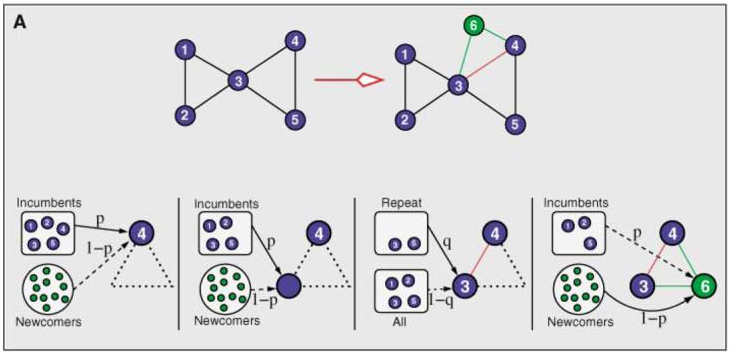
\includegraphics[width=0.8\textwidth]{guimera2}
	\caption{Probability-based team formation algorithm \cite{guimera2005team}.}
	\label{fig:ta2}	
\end{figure}

On the figure \ref{fig:ta2} depicted the probability-based team formation algorithm. $p$ is the probability for new members, $q$ -for group members \cite{guimera2005team}.
The authors of \cite{guimera2005team} assess the impact of the internal structure of the team on its expansion.

In \cite{moe2009overcoming} it is noted that the main factor for self-organization of teams is individual competencies.
The competencies of each participant are evaluated regarding usefulness for achieving the goal. 
In studies \cite{berger1972status, berger1980status} it is argued that such an assessment leads to the emergence of a system of statuses of team members, which is expressed in the hierarchy of communications. 
For the present study, it is sufficient that:
\begin{enumerate}
	\tightlist
	\item the goal is forming the basis for the team;
	\item the goal demand for the competencies of team members;
	\item participants assess each other's competencies to achieve a goal.
\end{enumerate}

The fundamental algorithm of team formation for two participants can be represented as the following time sequence (\ref{tab:ta1}):

\begin{table}[H]
	\centering
	\caption{Team flow.}
	\label{tab:ta1}
	\resizebox{0.95\textwidth}{!}{%
		\begin{tabular}{|l|l|l|}
			\hline
			\textbf{Step} & \textbf{Action} & \textbf{Result} \\ \hline
			One & \begin{tabular}[c]{@{}l@{}}The competences and experience necessary\\ for the achievement of the goal are defined.\end{tabular} & The goal \\ \hline
			Two & \begin{tabular}[c]{@{}l@{}}The first member of the team self-evaluate \\ hist competences and experience to the goal.\end{tabular} & The first member \\ \hline
			Three & \begin{tabular}[c]{@{}l@{}}The first member decided to create \\ a team for the goal.\end{tabular} & The team with one participant created \\ \hline
			Four & \begin{tabular}[c]{@{}l@{}}The second participant learns from \\ the first participant about the scope of the goal.\end{tabular} & The goal has not covered by the competences yet. \\ \hline
			Five & \begin{tabular}[c]{@{}l@{}}The second participant evaluate \\ the rest of the required competences.\end{tabular} & \begin{tabular}[c]{@{}l@{}}The competences of the second \\ participant are in demand for the goal.\end{tabular} \\ \hline
			Six & \begin{tabular}[c]{@{}l@{}}The second participant \\ decide to join the team.\end{tabular} & The team has two members. \\ \hline
		\end{tabular}
	}	
\end{table}

Shown in table  \ref{tab:ta1} sequence describes the main action of assembling the team.
We can say that after joining the team members have their profile of competencies to achieve a given goal. 
The team competencies are a superposition of competencies of the participants. 
The experience of the participants covers some of the competencies required to achieve the goal, and some are not.

The second participant joins the team with the set of competencies different from the first participant. 
For the convenience of the further notation let us formulate the following statements:

\begin{itemize}
	\tightlist
	\item Employees team up to achieve the goal;
	\item Team competencies are a function of the competencies of the participants;
	\item The unification of the first participant with the team to achieve the goal takes place on the same principles as the union team of $n$ participants with $n+1$ participant.
\end{itemize}

Let us consider the phenomena of the uniting of the first and second participants in more detail. 
The organizational environment defines the dimension $N_{comp}$ of the competency space. 
Each participant of the organizational environment $a$ has a vector of competencies $c_i$ such that $i \in N_{comp}$. 
The experience  $e_i$ characterizes each competence  $c_i$. 
The participant's experience is a natural number, $e_i \in \mathbb{N}$. 
As a result, we can say that the participant has a vector of experience in the competence space. 
Note that the competence space of the organizational environment has a significantly larger dimension than the vector of competencies of the participant.
Initially, the team $t_0$  does not contain participants and does not have its competencies (Fig. \ref{fig:ta3}).

\begin{figure}[ht]
	\centering
	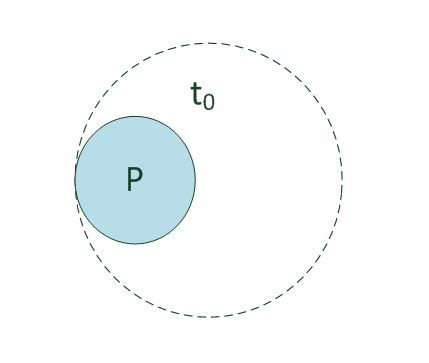
\includegraphics[width=0.5\textwidth]{scrum_fig3}
	\caption{The scheme of the team without participants.}
	\label{fig:ta3}		
\end{figure}

Let $P$ denote the goal to unite the team, $c_j$ denote the vector of competences, and $e_j$ denote the experience for each competence required to achieve $P$. 
As a result of successful uniting, the $t_1$ team will be formed for the achievement of the goal (Fig. \ref{fig:ta4}).

\begin{figure}[ht]
	\centering
	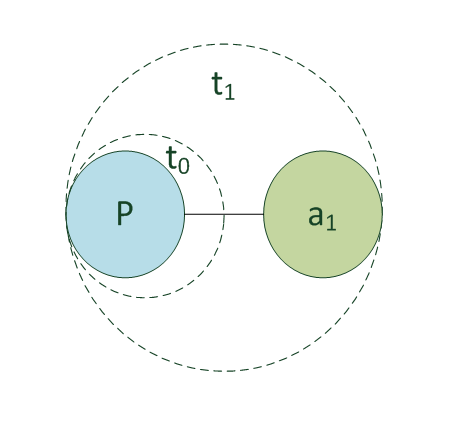
\includegraphics[width=0.5\textwidth]{scrum_fig4}
	\caption{The scheme of the team with one participant.}
	\label{fig:ta4}
\end{figure} 

The team $t_1$  has a new vector of competencies. 
Since $t_1$  has one participant $a_1$, then the vector competence $t_1$ is the same as the vector of competences of $a_1$. 
The team $t_2$ will be formed when participant $a_2$ joining team $t_1$  as shown in figure  \ref{fig:ta5}.

\begin{figure}[ht]
	\centering
	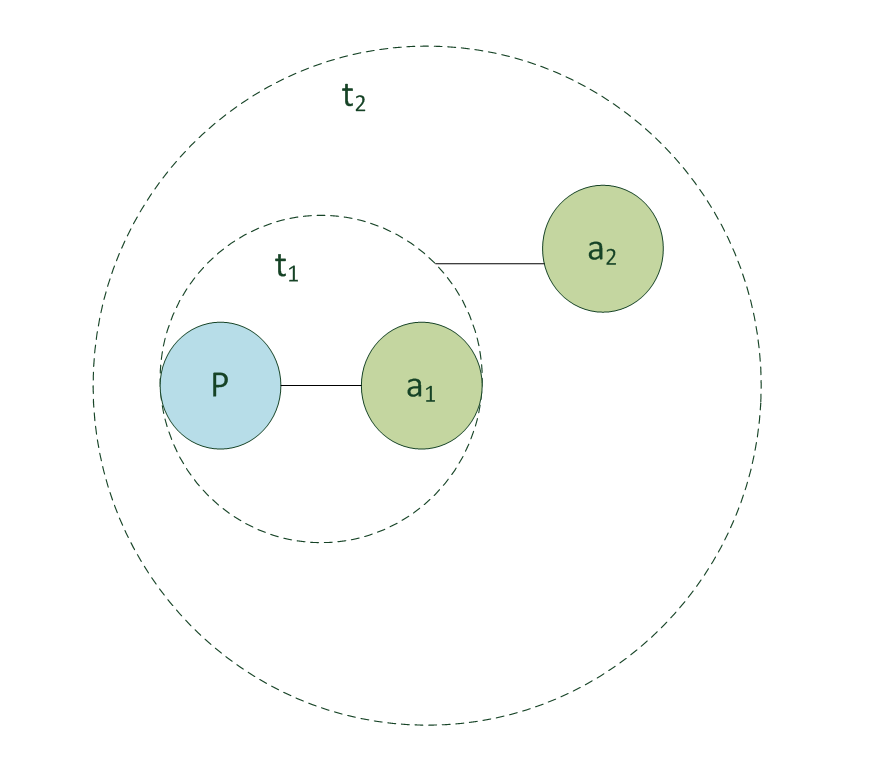
\includegraphics[width=0.6\textwidth]{scrum_fig5}
	\caption{The scheme of the team with two participants.}
	\label{fig:ta5}
\end{figure} 

Since the participant joins all elements of the team, it is possible to bring the scheme (Fig. \ref{fig:ta5}) to the form of the team graph (Fig. \ref{fig:ta6}).

\begin{figure}[ht]
	\centering
	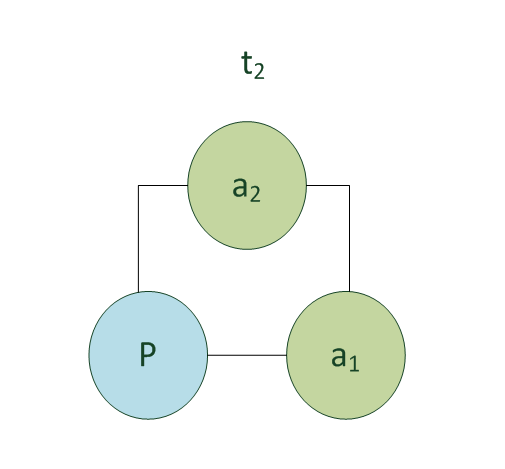
\includegraphics[width=0.6\textwidth]{scrum_fig6}
	\caption{The graph of the team with redundant connections.}
	\label{fig:ta6}	
\end{figure}  

The goal $P$ is an attribute of an edge linking $a_1$ and $a_2$.
We can convert the team graph with two members to an equivalent graph shown in the figure \ref{fig:ta7}.

\begin{figure}[ht]
	\centering
	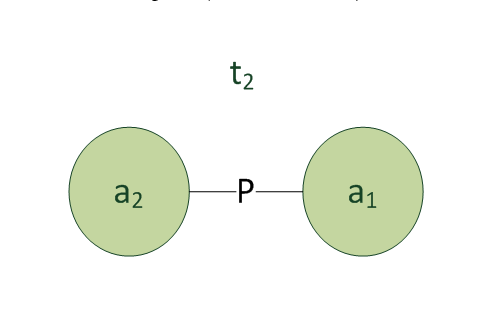
\includegraphics[width=0.6\textwidth]{scrum_fig7}
	\caption{The graph of the team with two participants.}
	\label{fig:ta7}
\end{figure}  

For the case of writing scientific articles, the graph of the team  $t_2$, shown in figure \ref{fig:ta7} denotes $g(t_2)$ and is called a co-authorship graph, where goal $P$ implies a scientific paper.
There is no information about the history of the team assembling in this notation. 
An example of a fragment of a co-authorship graph shown in the figure \ref{fig:ta8}.
The vertices of the graph are the researchers, and the edges are the joint scientific publication. 
The co-authorship graph is an undirected network.

\begin{figure}[ht]
	\centering
	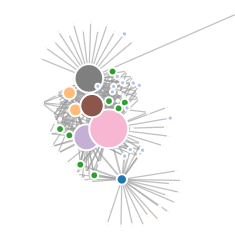
\includegraphics[width=0.5\textwidth]{scrum-img8}
	\caption{Fragment of a co-authorship graph.}	
	\label{fig:ta8}
\end{figure}  

Note that often for clarity the size of vertex reflects number of scientific articles written by the participant.

\subsubsection{Team code}

Let us introduce the concepts of \emph{Full Team Code (FTC)} and \emph{Residual Team Code (RTC)}.
These concepts play a crucial role in the formation of the team. 
The ingredients of the team code are competencies. 
By its type \emph{Full} and \emph{Residual} \emph{Team Code} are vectors in the space $N_{comp}$ .

Consider how a participant evaluates his competences for the needs in competencies for achieving the goal.

The characteristics of the goal $P$  are the basis for the formation of the team. 
That is, the first team member $a$ and the goal $P$ should be combined based on the concept of competencies. 
In other words, the necessary conditions for achieving the goal should be the possession of a $a$ specific set of competencies and experience. 
Concerning sets of employee competence $a$ and goals $P$ should be in the same space and have intersections. 
The presence of the intersections will lead to a team.

Let us introduce the evaluation function as $\Phi (P,t,a), \Phi \in [0,1] $. 
The result $\Phi$ be the probability of connection of participant $a$ to the team $t$ for the goal $P$. 
Then the function $\Phi$ for $n$-th participant can be written as $\Phi_n (P,t_{n},a_n)$.

As the participant joins, the team's competence vector will change.
It will include the competencies of new participants, and experience on the same competencies will develop (\ref{eq:scrum1}).

\begin{equation} 
\label{eq:scrum1}
ut_{n-1} = \prod_{a_j}^{a_{n-1}}\sum_i^{N_{comp}}\bigg\{c_j * \, e_i \bigg\}
\end{equation}

The value of $ut_{n-1}$ will be called \emph{Full Team Code (FTC)}. 
The \emph{FTC} characterizes the team's potential to achieve goals.

Expression \ref{eq:scrum2} represents the function $\Phi$ following the above algorithm \ref{tab:ta1}.

\begin{equation} 
\label{eq:scrum2}
\Phi  = P \cdot \prod_{a_j}^{a_{n-1}}\sum_i^{N_{comp}} \bigg\{c_j *\, e_i \bigg\} \cdot a_n
\end{equation}

An important semantic part in the expression \ref{eq:scrum2} carry out the component $rt^P_n$, which the author calls \emph{Residual Team  Code} -- \emph{RTC}. 
The expression for \emph{RTC} is \ref{eq:scrum3}.

\begin{equation} 
\label{eq:scrum3}
rt_n^P  = P \cdot \prod_{a_j}^{a_{n-1}}\sum_i^{N_{comp}} \bigg\{c_j *\, e_i \bigg\}
\end{equation}

The \emph{RTC} $rt_n^P$ characterizes uncovered  $t_n$ team competence for the goal  $P$. 
The zero vector as \emph{RTS} characterizes the complete staffing of the team's competencies to achieve the goal.
Now we can convert the expression \ref{eq:scrum2} to a more appropriate view \ref{eq:scrum4}.

\begin{equation} 
\label{eq:scrum4}
\Phi  =  rt_n^P \cdot a_n 
\end{equation}

The expression (\ref{eq:scrum4}) has an intuitive meaning: 

\emph{In order to assess the possibility of joining the team, the new participant must find out whether he/she has the necessary experience in the required competencies to fulfill the goal, taking into account that the existing team has already closed some of the necessary competencies with its experience}. 

In the works of \cite{hamilton2003team, prat2002should} this principle of team formation is called complementary.

\subsubsection{Team homogeneity}

We have considered the formation of teams by complementarity (complementarity) of competencies. 
The second driving force for the formation of teams is homogeneity.

The homogeneity of groups in social networks, or the propensity of people with similar characteristics to form links between themselves, also called hemophilia, is an essential factor in the formation and evolution of social networks \cite{mcpherson2001birds}. 
Many studies observed dynamic structure hemophilia \cite{snijders2010introduction,steglich20108}, which occur in parallel two processes.
On the one hand-similar individuals form social connections (social selection). 
On the other hand, people who are already connected adopt each other's behavior (social influence).
The combination of these factors results in a homogeneous social system in which there is a connection between individuals with similar behavior and characteristics, and the nature of the connection can be both formal and informal.

Although connections between individuals with similar characteristics are more likely than connections between different ones, the level of similarity is also essential.
In work \cite{block2014multidimensional} it was shown that social similarity by more than one indicator leads to the fact that people are less likely to form relationships with each other. 
The author explains this effect by the fact that people who are too similar in many characteristics, as a rule, cannot bring something new and constructive into a mutual relationship or a team.
Productive cooperation requires not only the similarity of interests but also different professional and life experience, which allows us to offer multidimensional approaches to its solution.

The main unifying factor in the team is the competence of the participants that affect the achievement of the goal.
Based on the concept of \emph{RTS} introduced earlier, we can consider the residual competencies of the participant, that is, competencies that are not required to unite the team to achieve the goal. 
The influence of this part of competencies on the team can both strengthen it and weaken it during work.

\subsubsection{Team work}

The team members define the beginning of work to achieve the goal, and it does not depend on the process of team formation. 
Only a running team may have performance indicators. 
For example, an important for the scientific domain term  ``scientific capacity''  means nothing more than the work performed by a team that has not empty \emph{RTS}.

Formation of the central system of internal interaction within the team according to the study \cite{harper1985power} occurs when meeting participants.
Thus, for this study, the author will ignore the time of establishing stable operation of communication channels.

In agile methods of software development, the most attention is paid to communications within the  team  \cite{boehm2003people} and with external agents \cite{paasivaara2012experiences}, which are mostly also a team, but in a broader sense.

The author formulates the following statement:

\textbf{Characteristics of communication channels correspond to the nature of the team.}

Thus, measuring the work of communication channels can make conclusions about the nature of the team.
Note a necessary consequence: this type of measurement of team performance does not create an additional burden on employees, in contrast to the methods of evaluation based surveys.

The question of measuring the contribution of individual participants or the result of the team is considered in many works \cite{tannenbaum2013team,hill1982group}. 
All researchers emphasize the fact that we need to measure both, team performance, and individual performance.
The study \cite{tims2013job} shows the following measurement scheme (Fig. \ref{fig:ex9}).

\begin{figure}[ht]
	\centering
	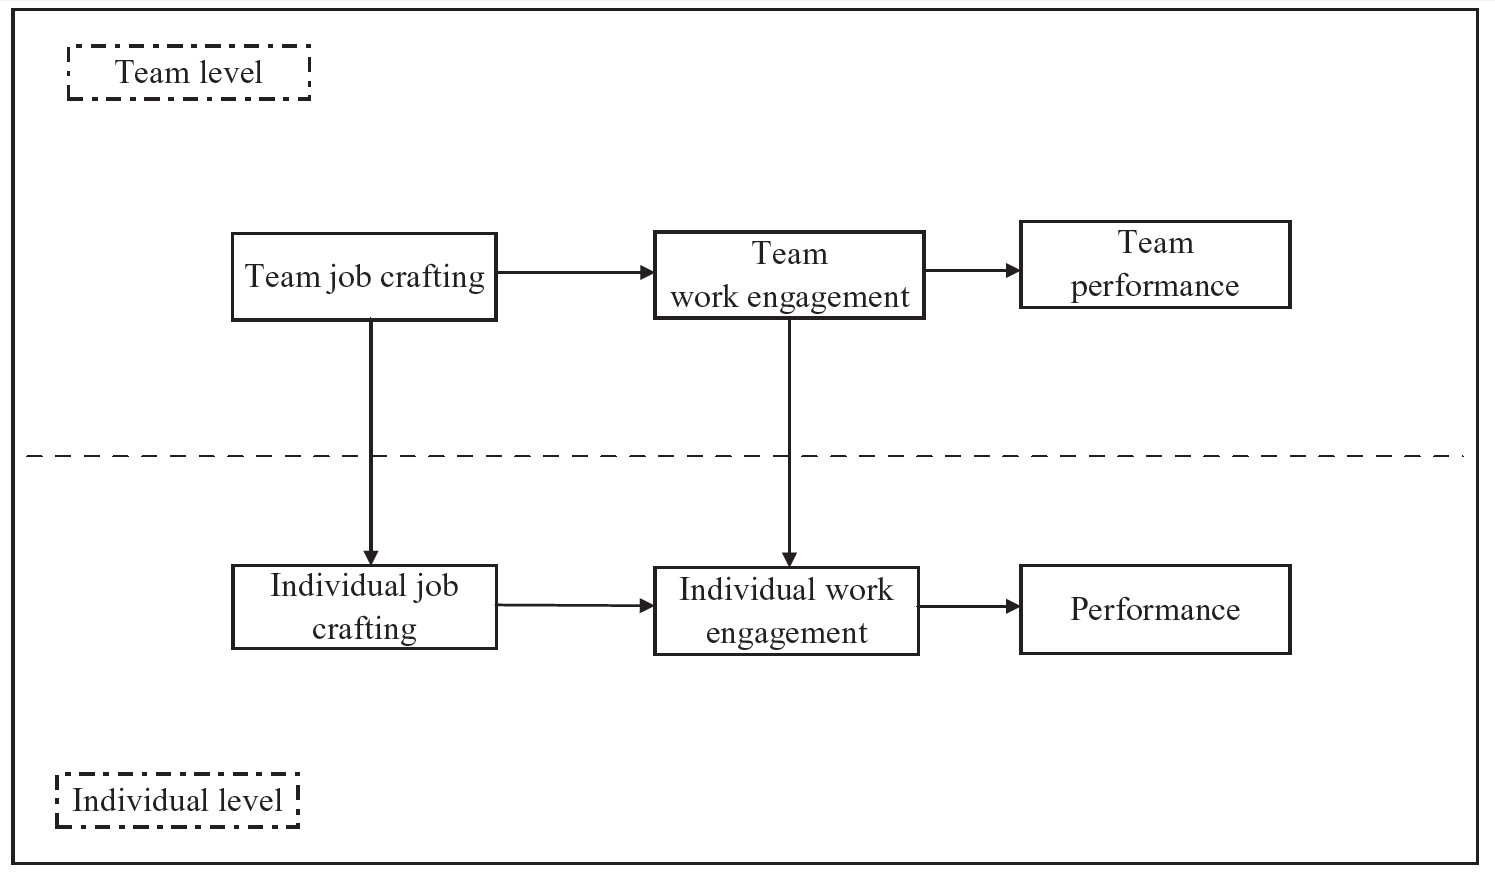
\includegraphics[width=0.8\textwidth]{scrum-img9}
	\caption{Team and participant performance measurement levels \cite{tims2013job}.}
	\label{fig:ex9}
\end{figure}

For example, the measurement of Individual Performance through surveys is explored in \cite{cropley2012measuring} by introducing Creative Solution Diagnosis Scale (CSDS) -- a scale of creativity. 
Measure the individual performance of an employee on such a scale the authors of \cite{cropley2012measuring} suggest using the Consensual Assessment Technique, which requires additional effort from employees.
The strengths and weaknesses of the survey method for measuring Individual Performance are outlined in the fundamental work of \cite{jackson1965person}.

The question of the method of measurement of Individual Performance finds an interesting statement in the modern concept of ``sensible organization'' \cite{olguin2008sensible}.
The authors of the \cite{olguin2008sensible} study, in addition to measuring traditional digital communication channels, put bracelets on employees that track movements and other body parameters.

The problems of the dependence of the team performance on the team structure are considered in the study \cite{kradoya2016structure}.

\subsubsection{Scrum Methodology}
One of the most common agile practices of teamwork is Scrum \cite{sutherland2013scrum}. 
Scrum is designed to produce the best possible results for team development of complex, intelligent products.
There are three fundamental roles in classic Scrum:

\begin{itemize}
	\tightlist
	\item Product owner - responsible for compliance with the objectives;
	\item Scrum master - responsible for the effective interaction in the team;
	\item Development team.
\end{itemize}

The recommended size of the Scrum team -- 5-7 people corresponds to the limitations of this study.
According to the ideology of Scrum \cite{sutherland2013scrum}, larger team require significant resources to communications, while the smaller size teams reduce the size of work that a team can complete per unit of time.

The basis of Scrum is Sprint, during which team creates the product. 
Sprints have the same duration throughout the product creation processes, one week is recommended. 
The task of Sprint is to materialize the product in its current form. 
In this study, the product is a scientific article.

The Scrum methodology declares the need for certain activities that are not related to research and writing text, which lead to better results. 
Also, Scrum sets a specific beat for these additional activities.

Let us introduce indicators that are affected by the application of Scrum to the process of writing scientific articles:

\begin{enumerate}
	\tightlist
	\item accelerate the exchange of messages in the communication channels;
	\item duplication in the absence of timely communication on research progress;
	\item non-compliance of the written article with the publication rules.
\end{enumerate}


From the formalism of the graph of co-authorship application of Scrum would lead to the selection of vertices of the graph provides the functions \textit{Product owner (PO)} and \textit{Scrum master (SM)} (Fig.\ref{fig:ex10}).

\begin{figure}[ht]
	\centering
	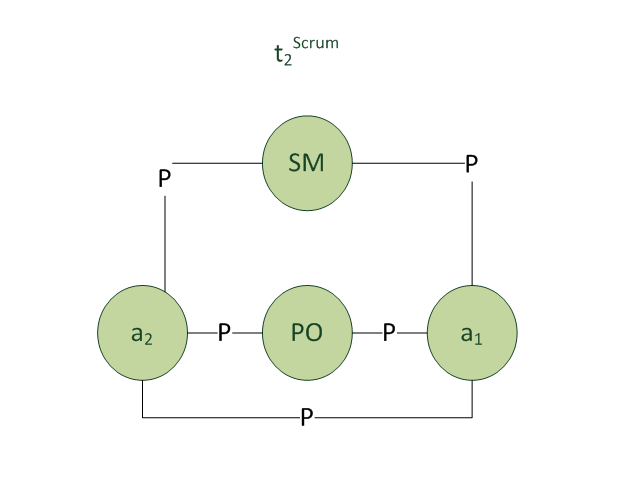
\includegraphics[width=0.8\textwidth]{scrum_fig10}
	\caption{The co-authorship graph with Scrum roles.}
	\label{fig:ex10}
\end{figure}  

With the graph $g (t_2^{Scrum}$) shown in Fig.\ref{fig:ex10} we can perform the conversion similar to the one made above with the graph $g(t_2)$. 
As we can see, the Scrum roles of PO and SM connect the vertices $a_1$ and $a_2$. 
It follows that PO and SM are the characteristics of the edges of the graph connecting $a_1$ and $a_2$. 
The transformed graph of co-authorship using Scrum roles is shown in Fig. \ref{fig:ex11}.

\begin{figure}[ht]
	\centering
	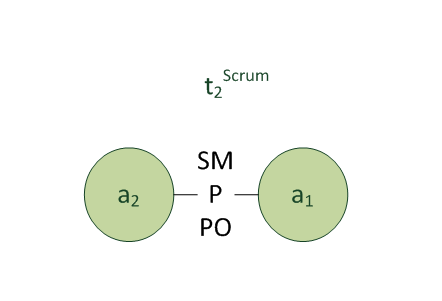
\includegraphics[width=0.5\textwidth]{scrum_fig11}
	\caption{The co-authorship graph with Scrum attributes.}
	\label{fig:ex11}
\end{figure}  

The role of Scrum according to \cite{fowler2001agile} should not interfere in the substantive work of the team, but only to speed up information exchange and to eliminate information barriers.
We formulate this as a hypothesis, the formal proof of which is postponed for further research:

\textbf{The introduction of Scrum roles in the co-authorship process does not change the appearance of the co-authorship graph.}

Now consider the performance indicators of the teams.

\subsubsection{Team performance metrics}

In modern work \cite{pereme2016toward}, considered the development of indicators that measure the rate of transition of the product from the research phase to the development phase. 
Authors of \cite{pereme2016toward} proposed an integral model for such indicators.  
They consider knowledge to be the object of measurement, and indicators are based on the Knowledge Management process.  
They did not offer any specific KPIs, but describe the spatial axes of their model such as processes, tools, and people.

The link between the team's ability to assemble and its productivity was investigated in \cite{edwards2006relationships}. 
It is worth noting that in \cite{edwards2006relationships} the assembling of a team implies the formation, not self-organization.

The composition of the team in time is not constant and say that the assembling of the team at one time or another time is not completed correctly.
Participants can leave a team and participate in several teams at the same time. 
An important milestone in the work of the team is determined by zero \emph{RTS} when the team members present all the competencies necessary to achieve the goal. 
Let us formulate this as statements:

\begin{itemize}
	\item \textbf{A team is complete if and only if its RTS is equal to the zero vector in the space $N_{comp}$.}
	\item \textbf{The minimum time in which the RTS became equal to the zero vector is called the Assemblance Time ($T_c$).}
\end{itemize}

Note that $T_c$ can be longer than the time allotted by the publishing house or the Program Committee of the scientific conference for preparation. 
Thus, the article will not have the required qualities in time and will not be accepted for publication.

Indicators that most accurately reflect the dynamics of the work will be based on changes in the dynamics of all parameters of the team. 
Let us introduce the function of the application of experience by the team in the competencies defined by the goal: $E (P,t)$.
Factors that negatively affect $E$ will be the complexity of communications $\Xi(g)$ within the team and the need to engage in activities not aimed at creating scientific articles:  $\Gamma(t)$.

Both $\Xi(g)$ and $\Gamma (t)$ will increase the time required to write a scientific paper.
Thus, the team may not achieve the goal in a particular time.

Let's formulate two considered reasons for not achieving the goal by the team:

\textbf{Abandoned Scientific Article (AAA) will be recognized as an article that does not meet the time frame of the publication process with the required quality.} 

The ratio of the number of abandoned articles ($Frac_{notpub}$) to the number of published articles is an indicator of the performance of the process of writing scientific articles.

Another more obvious performance indicator is the time taken to publish a scientific paper $T_{pub}$.

\section{Text Analysis }

Let us consider text mining and analytics (TM\&A). 
The mission of TM\&A is to turn text data into high-quality information or actionable knowledge.
Concerning this mission there are two important conditions would be mentioned.
\begin{enumerate}
	\item Minimization of human effort (on consuming text data);
	\item Supplying knowledge for optimal decision making.
\end{enumerate}

Related to text retrieval, which is an essential component in any text mining system we must note that:
\begin{enumerate}
	\item Text retrieval can be a preprocessor for text mining;
	\item Text retrieval is needed for knowledge provenance.
\end{enumerate}

The broad picture of TM\&A is shown in figure \ref{fig:tm1}.

\begin{figure}[ht]
	\centering
	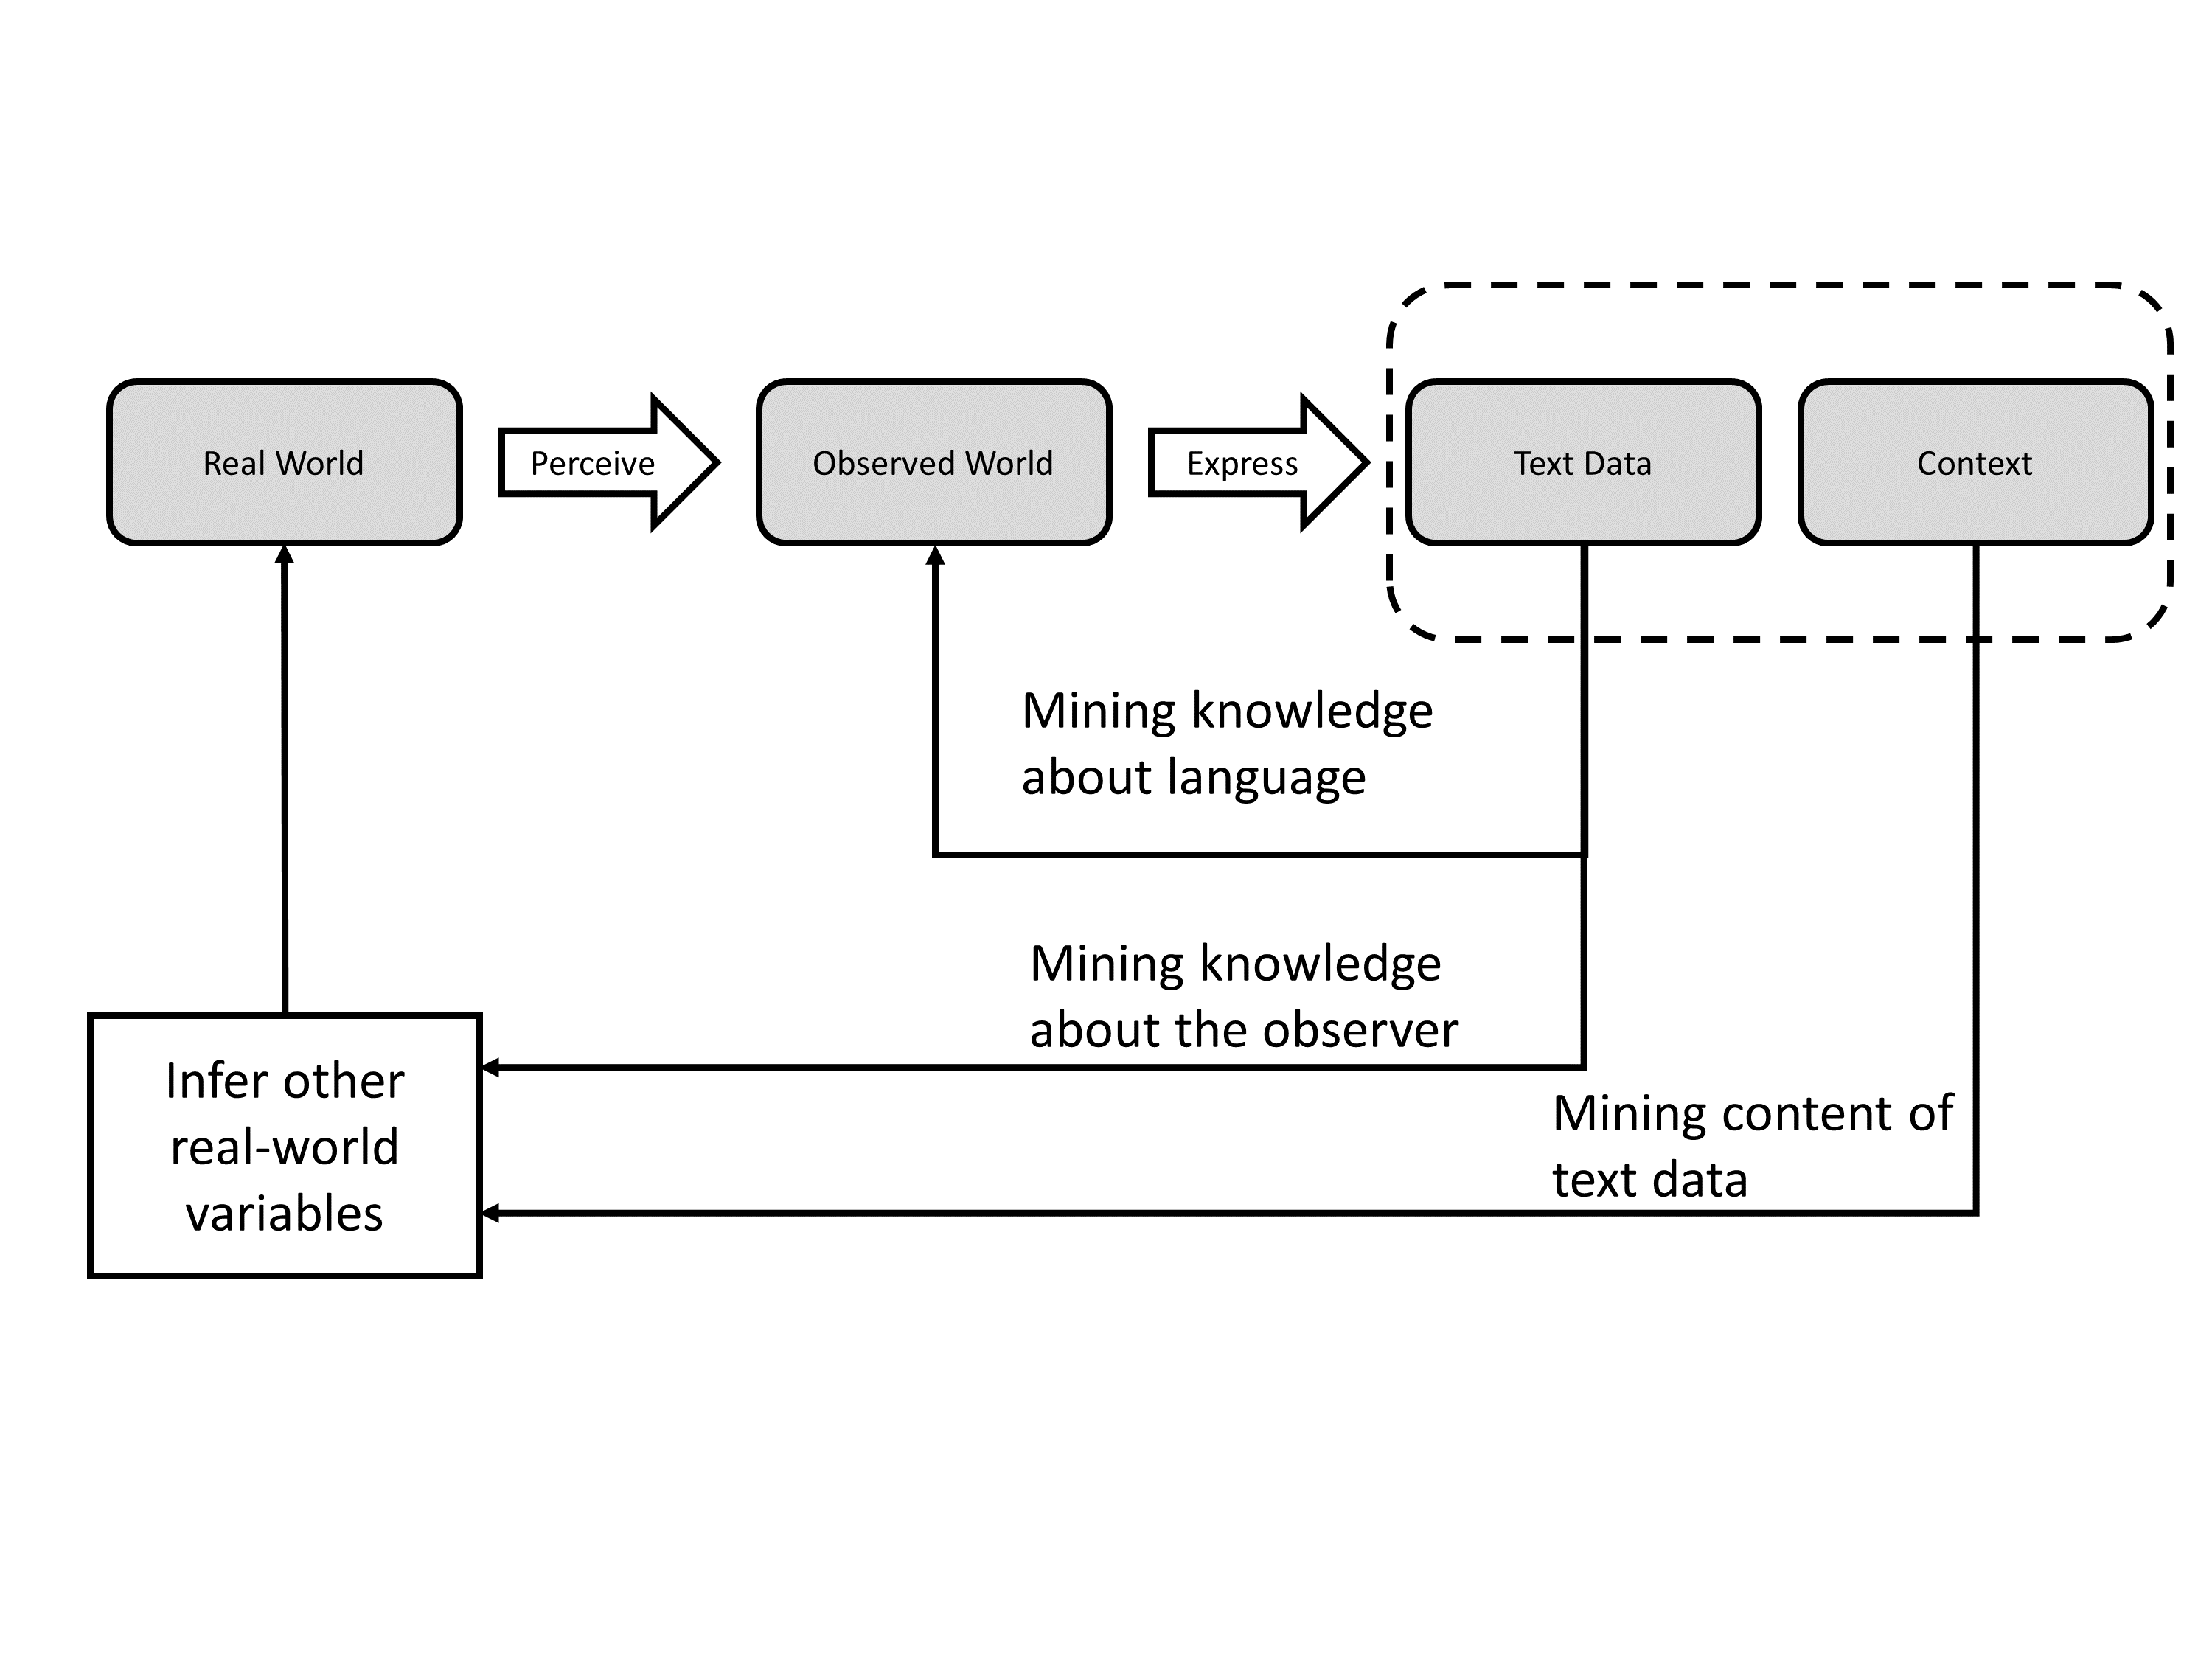
\includegraphics[width=0.9\textwidth]{tm1eng}
	\caption{Landscape of Text Mining and Analytics.}
	\label{fig:tm1}
\end{figure}  



\subsection{Topic Detection}\label{sec:topicmodel}

In recent years, the methods of topic modeling are rapidly developing. Recent studies have led to the development of several main areas: probabilistic [1], based on SVD [2] and generative [4].
Topic modeling defines each topic as the distribution of a certain number of words with specific probabilities. 
Most modern topic models are based on the Dirichlet distribution (LDA, Latent Dirichlet Allocation) [3].
It is hard to imagine that such a universal distribution as LDA would work adequately for any text. 
We need to fine-tune the algorithm for a specific problem domain. 
Therefore, the author focused on the primary world source for scientific and practical articles of the oil and gas industry - The OnePetro library. 
It is important to note that the OnePetro library covers a wide range of engineering disciplines and contains texts in English dedicated to the practical aspects of the application of new technologies in the oil and gas industry. 
The authors of the articles in the OnePetro are employees of oil companies from all over the world.

The precise formulation of the problem of topic modeling is as follows. 
Let fixed dictionary of terms $W$, from which elements are formed documents of given collection $ D $ containing documents $d \in D$. 
For each document $d$ its length $n_d$ and the number of $n_dw$ uses of each term $w$are known.
Let $\Phi=(\phi_{wt})$ be a matrix of term distributions $w$ in topics $t$, and $\Theta=(\theta_{td})$ be a matrix of topic distributions $t$ in documents $d$. 
Then the problem of thematic modeling is to find such matrices $\Phi$ and $\Theta$ that the equation is became valid (\ref{eq:op3_1}).

\begin{equation} 
\label{eq:op3_1}
p ( w \vert d ) = \sum_{t \in T} \phi_{wt} \theta_{td}
\end{equation}

In equation \ref{eq:op3_1} $ \phi_{wt} $ is the probabilities of the terms $w$ in each topic $t$, $\theta_{td}$ is the probabilities of the $t$ in each document $d$, and $ p ( w \vert d) $ is the probability of the term $w$ appearing in the document $d$.

The equation \ref{eq:op3_1} can be represented as $ \Phi \cdot \Theta $. 
It is easy to show that this problem has many solutions (\ref{eq:op3_2}).

\begin{equation} 
\label{eq:op3_2}
\Phi \cdot \Theta  = \Phi \cdot \Lambda \cdot \Lambda^{-1} \cdot \Theta = \hat{\Phi} \cdot \hat{\Theta}
\end{equation}

In equation \ref{eq:op3_1} $\hat{\Phi} = \Phi \cdot \Lambda $, and  $\hat{\Theta} = \Lambda^{-1} \cdot \Theta$.

It follows from the equation \ref{eq:op3_2} that the matrices $\hat{\Phi}$ and $\hat{\Theta}$ will also be solutions to the equation (\ref{eq:op3_1}).
But not all matrices $\Phi$ and $\Theta$  contain well-interpreted topics. 
Thus, the problem (\ref{eq:op3_1}) must enter the conditions which would produce adequate and exciting topics. 
Figuratively we can say that it is necessary to digitize the specificity of the subject area of the text for embedding in the algorithm of the search of optimal matrices $\Phi$ and $\Theta$. 
Note that when using LDA to create a thematic model, this setting is not made in the subject area.
For solving subtask configure the topic model for the subject domain, the author has used the mechanism of regularizers.

Let $p \left( t \right) $ be the distribution of topics in the document collection:

\begin{equation} 
\label{eq:op3_3}
p \left( t \right) = \sum_d p \left( d \right)  \theta_{td}
\end{equation}

Then it may be helpful to ad regularization based on the Kullback–Leibler divergence ($\mathcal{KL}$)  shown in \ref{eq:op3_4}.

\begin{equation} 
\label{eq:op3_4}
\mathcal{KL}(\Theta)= -\tau \sum_{t \in T} \ln \bigg( \sum_{d \in D} p \left( d \right) \theta_{td} \bigg) \rightarrow max
\end{equation}

Where $\tau$ is a regularization parameter to be chosen depending on the subject area of the document collection. 
The requirement of maximizing $\mathcal{KL}(\Theta)$ lead to the zero probability of the appearance of documents and the greater sparsity of the matrix $\Theta$.
The second mechanism for regularization may be the opposite - increasing the probabilities for topics that are present in many documents. 
Such subjects are called noise. 
To obtain the seals of the rows of the matrix $\Theta$ with noise subjects can apply regularization (\ref{eq:op3_4}) with the opposite sign. 
Thus, the matrix $\Theta$ after the regularization is to introduce an alternation of zones of sparsity for the major subjects and seals for noise topics. 

The resulting topic model should be formally checked for quality. 
Quality metrics of the topic model must be embedded in the learning process. 
Moreover, after reaching the formal convergence criteria of the model the history of metric evaluation needs to be visualized. 
The primary metric for detecting convergence of the topic model is the metric Perplexity calculated by the formula (\ref{eq:op3_5}).

\begin{equation} 
\label{eq:op3_5}
\mathcal{P}(D, \Phi, \Theta) = \exp \bigg( \frac{-1}{n_d} \sum_{d \in D}  \sum_{w \in d}  n_{dw} \ln \bigg( \sum_{t \in T} \phi_{wt} \theta_{td} \bigg ) \bigg)
\end{equation}

The Perplexity metric is not normalized and therefore cannot be used to compare the convergence of different models. 
The prevailing logic is that the smaller the Perplexity, the better the model. 
Therefore, to decide on sufficient convergence, the models are guided by the fact that Perplexity ceases to decrease significantly with the growth of the number of training iterations.

The resulting model of topics can be considered as a soft clustering. 
In this case, visualization tools used for clusters can be applied to the obtained topics. 
For example, manifold-based learning methods such as t-distributed Stochastic Neighbor Embedding (TSNE) and multi-dimensional scaling  (MDS) can be applied. 
The results of the TSNE algorithm depend on the chosen metric of the distance between the vectors. So we should find a suitable one.
When the dimension of the vector space in a few hundred use the following metrics:

\begin{itemize}
	\item 	Сosine distance: $ \frac{v_1 \cdot v_2}{\Vert v_1 \Vert_2 * \Vert v_2 \Vert_2 } $
	\item 	Euclidean distance: $ \Vert v_1 - v_2 \Vert_2$
\end{itemize}

To effectively use the visualization of the topic model with the help of learning methods based on manifold-based methods, it is necessary to present the words that make up the subject in Vector Space Model (VSP). 
This procedure is called word embedding. 
For it often uses the method GloVe described in the study \cite{pennington2014glove}. 
An alternative method of word embedding is FastText \cite{joulin2016bag}, so the author of this study decided to make a qualitative comparison of both methods of word embedding on the selected collection. 
Both methods learn vector representations of words based on how often words are used together. 
The difference between them is that FastText can be called ``predictive'', and GloVe is based only on the frequencies of words. 
In this light, GloVe is much simpler, and the author of this study believes that simplicity in business is the key to efficiency.

Library BigARTM \cite{ianina2017multi} allows you to build several regularizers and control groups of subjects consistently. 
This tool is unique at the time of writing this study. 
Widely used methods of constructing topic models based on LDA do not provide such opportunities.

\subsection{Sentiment Analysis}
Sentiment analysis of text is intended to detect in the texts of the emotionally charged vocabulary. 
Sometimes researchers distinguish the term ``Opinion mining'', thus emphasizing the task of searching in the texts of value judgments. 
In addition to the academic study of the tone of the text as one of the sections of computer linguistics, there are some applied studies aimed at improving the management decision-making process.

The use of recurrent and convolutional neural networks for sentiment analysis made it possible to achieve much higher accuracy compared to models based on logistic regression.

The author focused on the method of choosing the optimal architecture and hyperparameters of the neural network, which allows training the classification model on a public dataset containing estimates, and then to predict the text fragments from scientific and practical articles containing estimates with a given degree of accuracy.

The methodological approaches applied by the author can be presented in the following research framework of the study (Fig. \ref{fig:op4_1}). 
Let us consider in more detail each of the elements of the systematic framework.

\begin{figure}[ht]
	\centering
	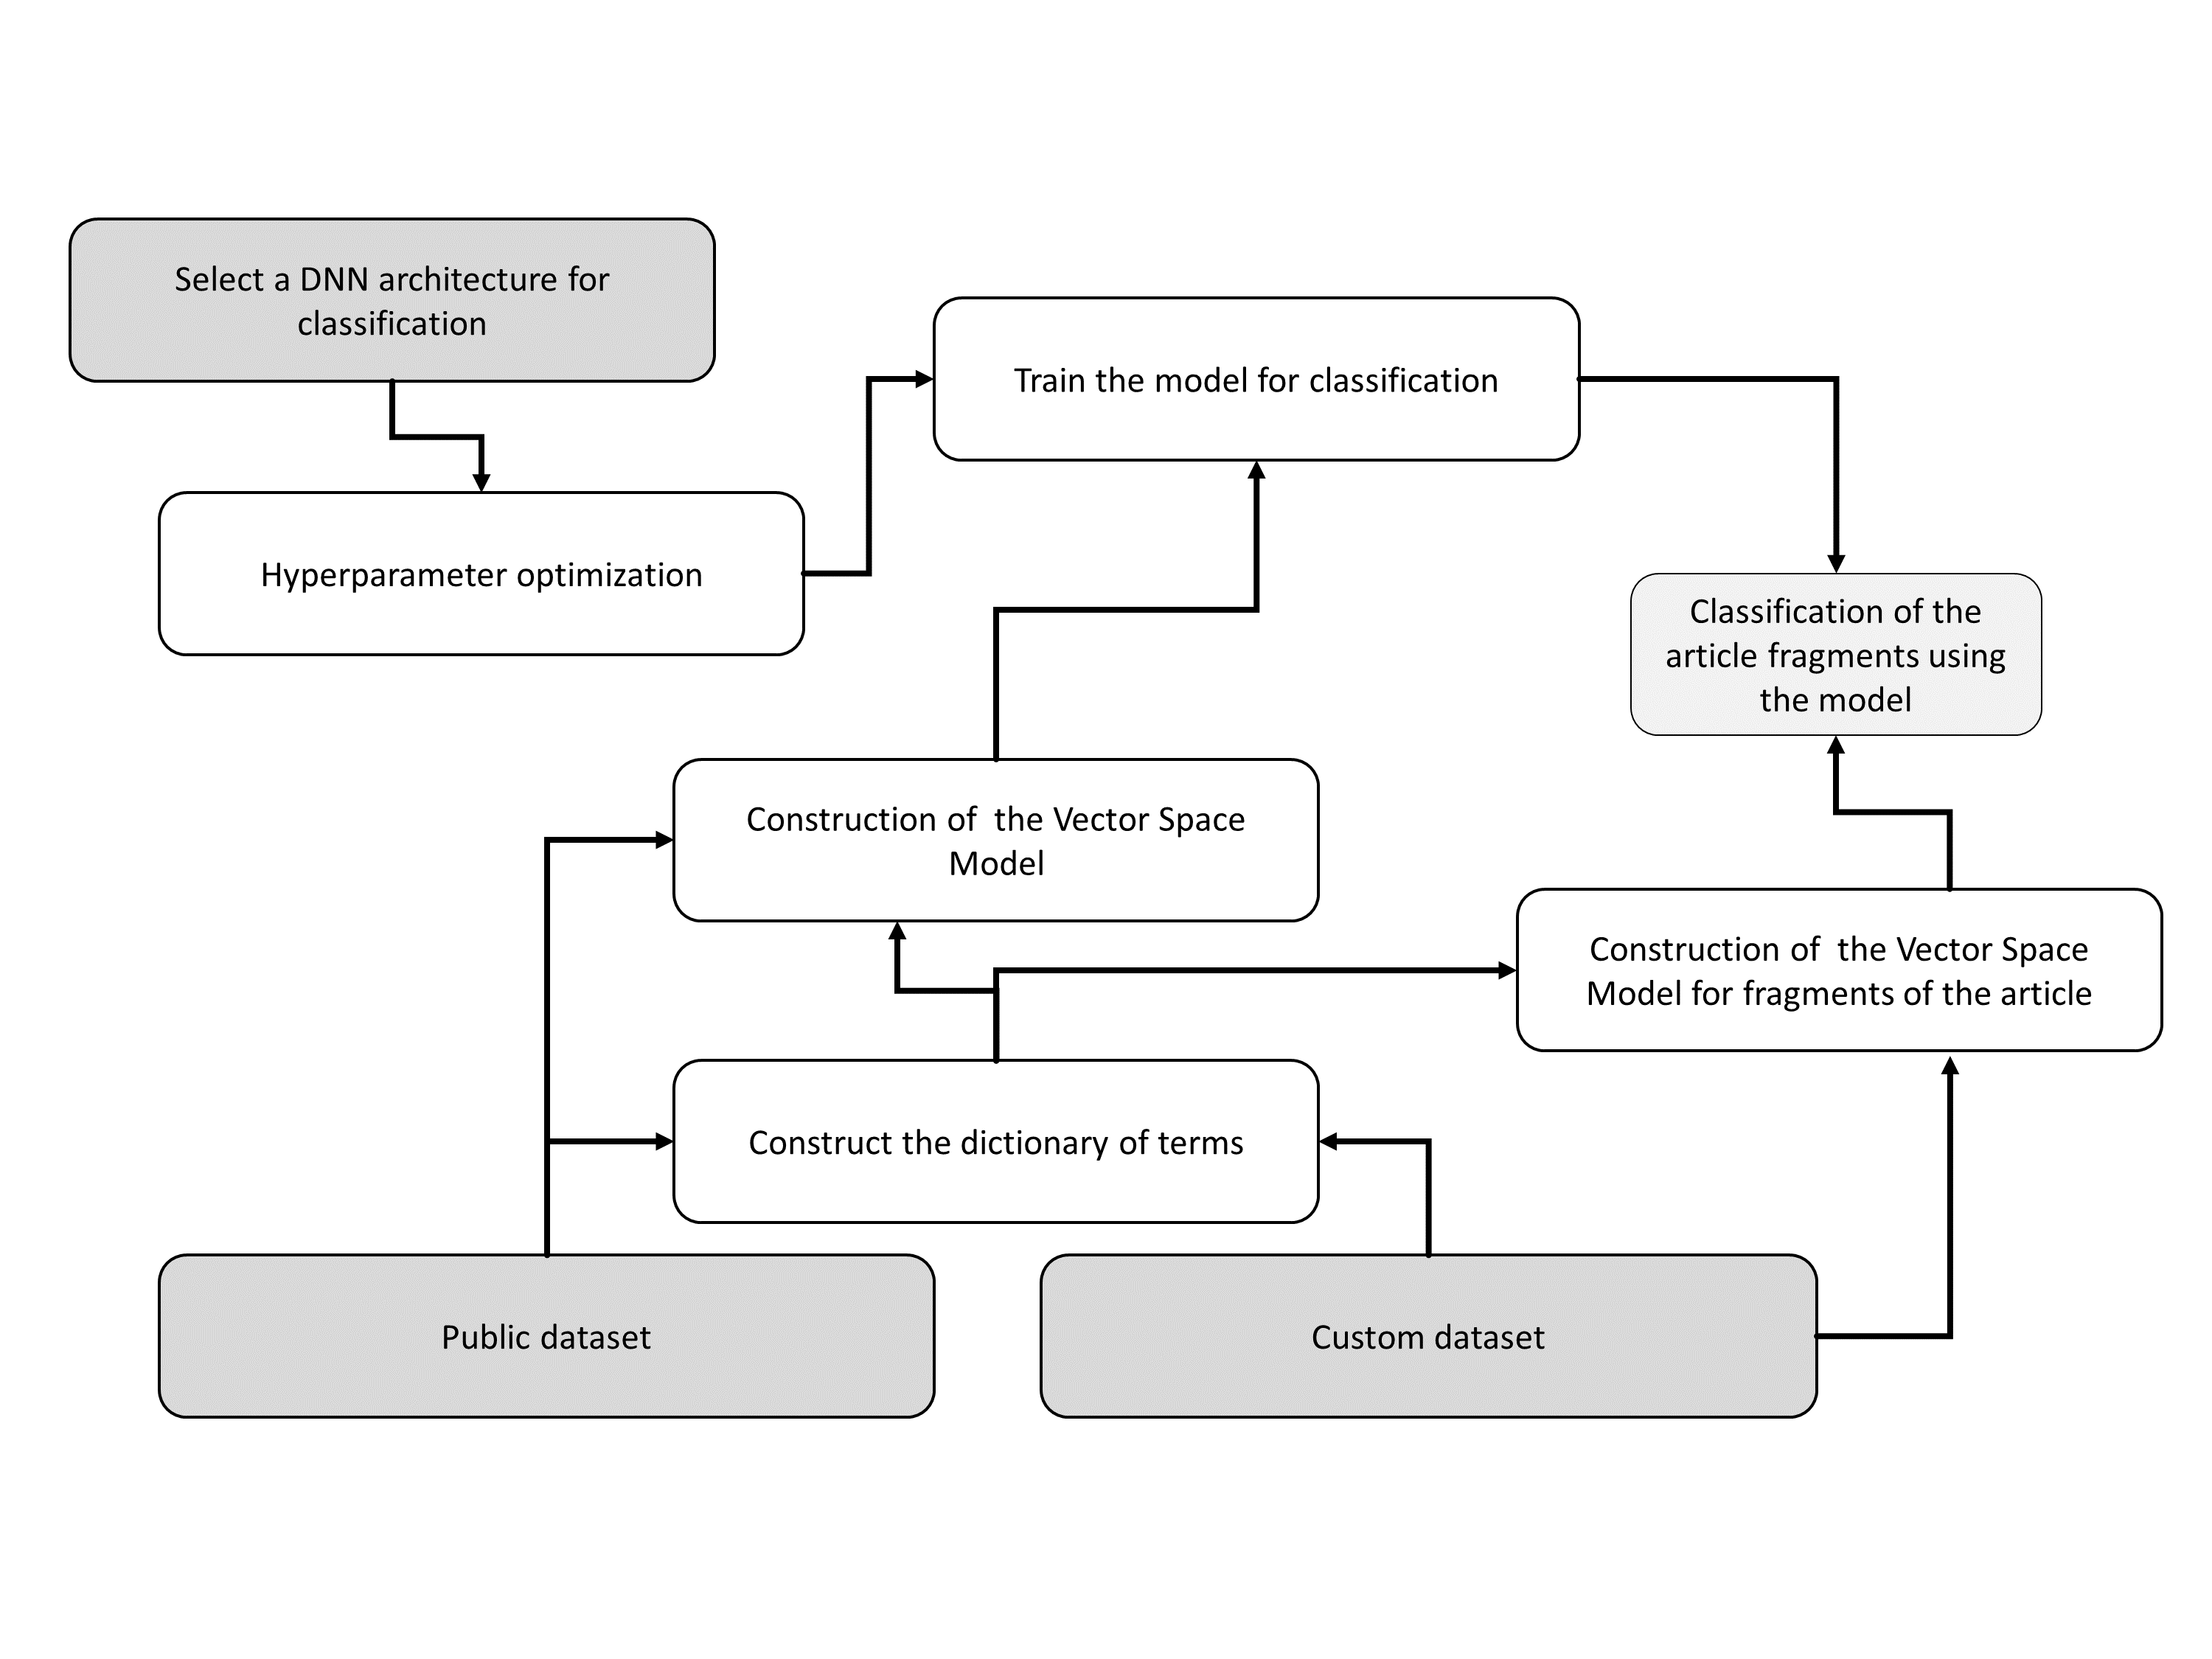
\includegraphics[width=0.9\textwidth]{op4_1eng}
	\label{fig:op4_1}
	\caption{Research framework for the study of emotional coloring of the texts.}
\end{figure}  

\chapter {Approbation and Results}
\section {The set for the experiment for direct and inverse problems.}

Two different domains are closely intertwined with each other and provide a comprehensive, in-depth look at the object of the study. 
Let us list these domains:

\begin{itemize}
	\item The study of the STC via external presentation,
	\item The study of the STC from the inside.
\end{itemize}	

These two tasks are oppositely directed. Let's take a closer look at them.

External manifestations include digital artifacts of the organization's activities - published scientific articles, conference materials, information sites on the Internet and news about the company.  
The study of digital artifacts is carried out using approaches based on the analysis of texts and co-authorship.

Then we are studying the STC from the inside; the research includes modeling of scientific activity, the efficiency of production processes, self-organization of small creative teams and models of scientific organization personnel.

Suppose we consider a particular organization with a certain
number of employees, budget and work plan. 
Our interests are in the roots of the effectiveness of this organization. 
From this point of view, the following issues are essential for us:

\begin{itemize}
	\item 
	What is the intellectual potential of the organization? 
	What research organization can perform independently, and which must be conducted in conjunction with other scientific organizations. 
	It is evident that when carrying out joint research, communication costs arise and the study needs additional coordination. 
	However, for efficiency is important not only the original boundary " can or can not," but also the distribution of time and effort.
	\item 
	Performance is known to degrade under high load conditions.
	However, for questions of efficiency, this effect must be considered in the dynamics, as the return from degraded to regular also takes time.
	Also, it is important to segment the load by employee type. 
	Beginners can be both overloaded and underloaded with work. 
	Depends on the turnover of staff. 
	However, a load of experts significantly more significantly affects the efficiency. 
	The effects of mental fatigue of experts dramatically affect the efficiency.
	\item 
	Scientific assets of the organization are exhausted? 
	What is the dynamics of creating scientific assets? 
	Are there any breakthrough trends in research conducted within the organization? 
	Who is involved in the creation of a scientific justification?
\end{itemize}

The parameters of the organization are impossible to measure. 
We need essential measuring instruments.
However, the effectiveness of STC depends on the parameters in principle. 
The methods of estimation of these parameters developed by the author give methodological approaches to the clarification of the above questions.

The direct method of measurement in this study is to simulate the dynamics of the organizational environment to obtain digital artifacts.
For this purpose, the author created personnel models, team building models, and STC productivity, models. 
The result of a multi-program experiment with these models is synthetic digital artifacts of the scientific organization: co-author, subjects, and directions of development. 

The inverse method of the experiment analyzes the real digital artifacts of the STC. 
Namely, scientific articles, conference materials and from digital artifacts, the author builds a model of co-authorship, models of scientific topics, models of scientific directions and scientific schools in the organization.

\section{The results of modeling of the process of publishing scientific articles}
\label{sec:di}
In this study, the publication activity of the scientific and technical center of Gazpromneft STC in the OnePetro electronic library of the  Society of Petroleum Engineers (SPE)\footnote{SPE is a not-for-profit professional organization  for oil and natural gas exploration and production (E\&P) professionals. It was founded in 1957, and today brings together more than 165,000 engineers, scientists, managers, and educators} was analyzed. 
The obtained dependence is shown in the figure (Fig. \ref{fig:om5}).

\begin{figure}[ht]
	\centering
	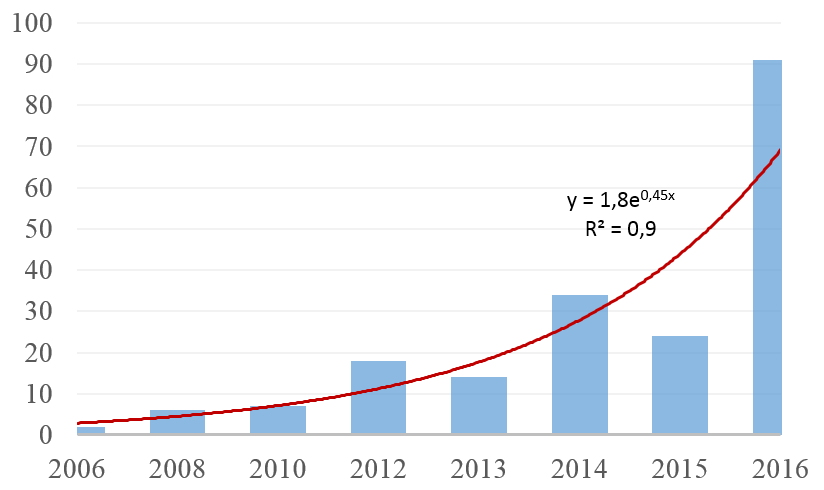
\includegraphics[width=0.8\textwidth]{om5}
	\caption{The number of publications of employees of Gazpromneft STC.}
	\label{fig:om5}
\end{figure}  

The exponential growth of publications in one edition cannot continue indefinitely. 
Each edition has its limit of publications, manuscripts coming over the permissible volume of publications, increase competition for the right to be published. 
However, as a result of selection, some high-quality manuscripts are rejected by publishers.
A simulation model was developed to study the publication process. 
The cognitive map of the publication process model is shown in the figure (Fig. \ref{fig:om6}).

\begin{figure}[ht]
	\centering
	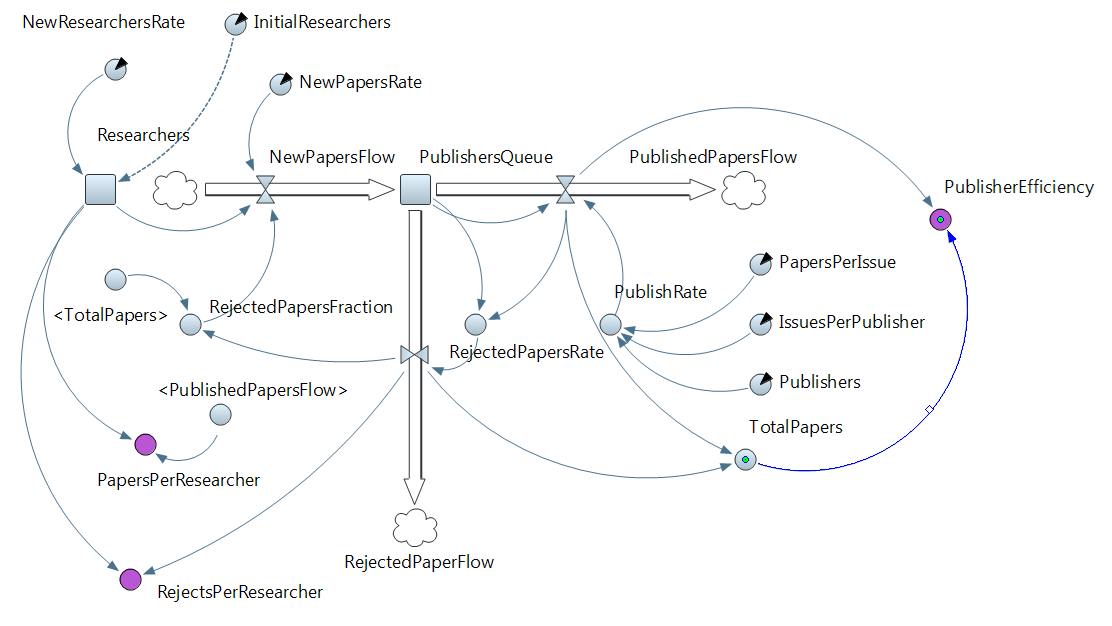
\includegraphics[width=0.8\textwidth]{om6}
	\caption{Cognitive map of the publication process model.}
	\label{fig:om6}
\end{figure} 

The created model of the publishing process contains two stocks:

\begin{itemize}
	\tightlist
	\item Researchers,
	\item PublishersQueue -- the stock of the manuscripts.
\end{itemize}

The model (\ref{fig:om6}) is controlled by the following free parameters (Tab. \ref{tab:om3}):

\begin{table}[H]
	\centering
	\caption{Free parameters of the publishing process model.}
	\label{tab:om3}
	\resizebox{0.7\textwidth}{!}{%
		\begin{tabular} {|l|l| }
			\hline
			\textbf{Parameter Name} & \textbf{Description} \\ \hline
			Publishers & The number of publishers \\ \hline
			PapersPerIssue & The number of articles in issue \\ \hline
			IssuesPerPublisher & The number of issues per publisher per year \\ \hline
			NewPapersRate & The speed of manuscripts creation \\ \hline
			InitialResearchers & The initial number of researchers \\ \hline
			NewResearchersRate & The rate of emergence of new researchers \\ \hline
		\end{tabular}%
	}
\end{table}

A digital experiment was conducted by the cognitive map of the publication process model.
Figure \ref{fig:om7} presents the dependence of the efficiency of the publications from time to time with the different number of publishers.

\begin{figure}[ht]
	\centering
	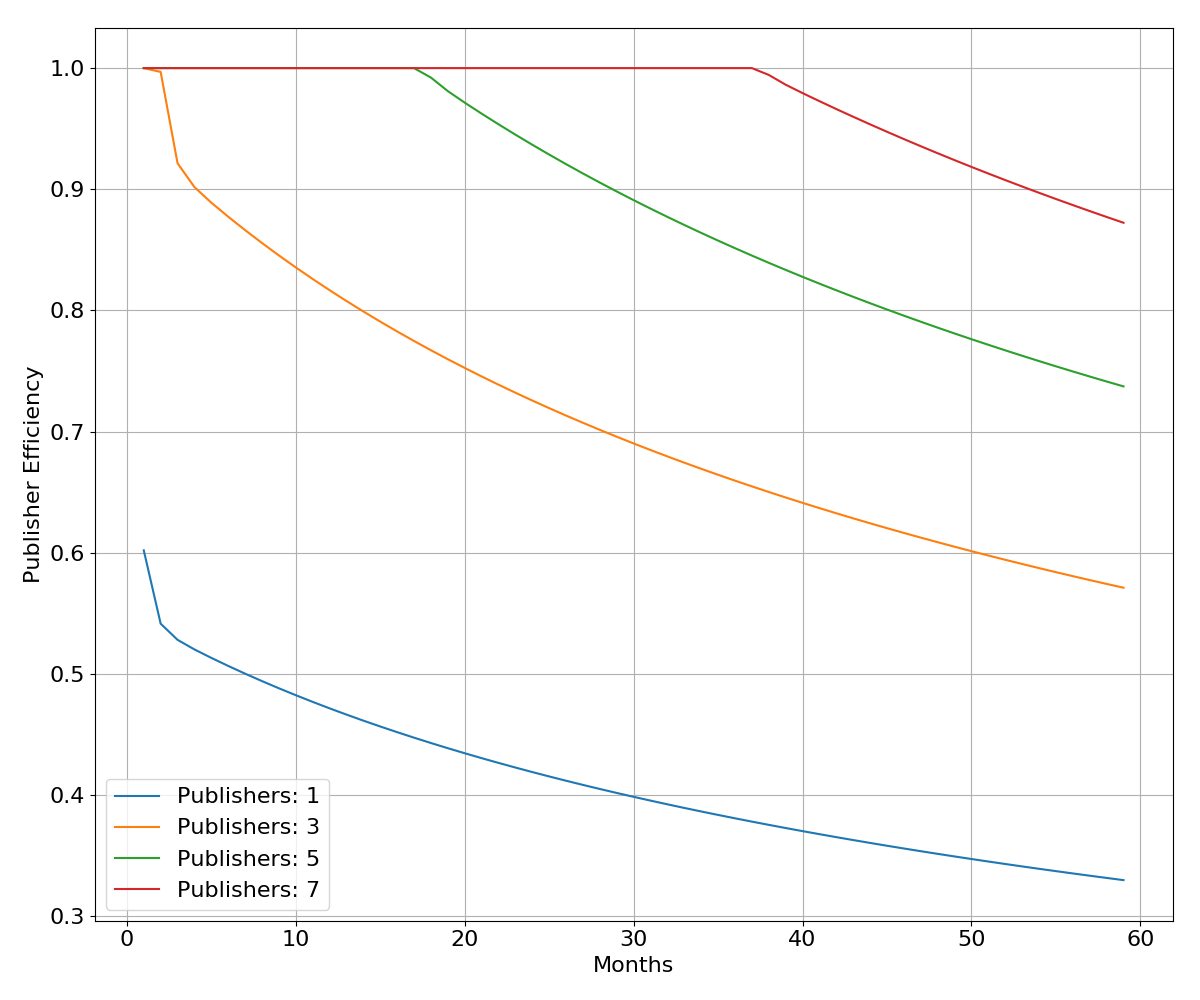
\includegraphics[width=0.8\textwidth]{om7}
	\caption{The curve of the effectiveness of publications  to time with a different number of publishers.}
	\label{fig:om7}
\end{figure} 

The decline in the effectiveness of publications, as we can see, has a sharp, avalanche-like character. 
This type of publication efficiency behavior requires special attention in order not to miss the beginning of stagnation and to take organizational measures to increase the number of publishers involved in the publication process.  

The principle of division of labor leads to an increase in the efficiency of processes. 
Hypothetically, extending the role model can improve the efficiency of the publishing process. 
Regardless of the number of co-authors, the publishing process defines the following roles:

\begin{itemize}
	\tightlist
	\item Producer -- the carrier of the main idea of the research;
	\item Editor -- changes the text of the manuscript;
	\item Reviewer -- is responsible for the conclusions and results of the study;
	\item Translator -- if the article is not in the authors' native language, technical translation and proofreading are required;
	\item Specialist in working with publishers -- responsible for finding publishers and external communication;
	\item Designer -- pictures, the presentation of the report;
	\item Speaker -- presents the result orally at the conference (if needed and as many times as needed);
	\item Data Scientist -- conducting computer calculations.
\end{itemize}

Given these roles, the research team does not change.
The authors of the study are the scientists who conducted it. 
The quality of the manuscript getting better, and communication becomes more professional. 
Note that the functions of external and internal corporate communications are usually present in the organizational environment, but do not focus on the individual needs of researchers.

\section{Measurement of the Intellectual Capital}
\label{sec:ic}
Intellectual capital (IC) by its nature is a composite indicator of the productivity of a research organization whose main product is knowledge.
The IC structure includes:
\begin{itemize}
	\tightlist
	\item Human capital 
	\item Organizational capital 
\end{itemize}

Human capital (HC) - includes knowledge and skills. 
Organizational capital (OC) includes technologies and processes. 
In other words, the HC characterizes the experience of employees, and the OC characterizes how employees apply their experience to the tasks in this organization. 

In addition to creating intellectual capital, we can also consider its destruction – employees who conducted research leave and take with them knowledge.

Employees' contribution to intellectual capital is not equal. 
Next, the authors define the roles that belong to the "core team". 
The loss of employees at the core of the team dramatically impacts performance. 
The core includes employees with a high level of experience and the most popular skills in the organization.

There are quite a few approaches that describe the life cycle of an employee within an organization or position, but most studies agree on four main stages regarding the level of productivity:

\begin{enumerate}
	\tightlist
	\item the initial stage, 
	\item the accumulation of experience, 
	\item the productive stage, 
	\item the productivity decline.  
\end{enumerate}

At the same time, the stage of adaptation (initial stage and accumulation of experience) may differ depending on the type of activity and position level, but on average it takes up to six months for specialists and middle managers, about a year for senior managers.

The highest percentage of turnover among newcomers, so more attention should be paid to the social adaptation of new employees, the integration of newcomers in the processes and mentoring.

When a creative team breaks up, the brain drain can be different and doesn't always harm performance. 
In other words, sometimes the departure of an experienced, but having a different from the majority of the mental model of the employee, reduces the growth constraints of the IC.

There are two cases of staff turnover by employee's resignation and employer-initiated. 
From the IC point of view, both components have a negative impact. 
In Russian practice, there is a stable concept of staff turnover: an indicator that records the level of change in composition as a result of dismissal and transition to another job for personal reasons. 
The concept of turnover usually does not include the transition of an employee to another employer through transfer, which significantly distorts the Russian results compared to foreign ones. 
In different industries and industries, as well as at different levels of management, various values of staff turnover (from 2-5 to 80\%) are considered the natural, which is due to the peculiarities of the business and categories of employees. 
For example, for retail and service sectors are characterized by very high rates of staff turnover, whereas for heavy industry, the standard relatively low value of staff turnover (5-10\%).
Typically, the level of staff turnover increases as the younger X-generations and Y-generations enter the labor market.

It is also important to note the relationship between burnout, fatigue and staff turnover, which has a negative impact on the productivity of the organization.
The staff turnover has positive feedback reduced productivity. 
Organizations with high turnover typically have more problems with productivity and IC accumulation. 

The most significant component of IC is the productivity of the organization, reflecting the ratio of effective staff to the total number of employees.  

The author of this study has built a model of the IC based on the productivity of the organization. 
As an input for the IC model, a staff model was also built.
The staff model usually solves the problem of predicting the number of personnel depending on the specific drivers of the population, usually an external (number of projects, tasks, customers, objects, services) from the current or specified productivity.
The main problem of the staff models developed by the organizations, is a linear dependence of the personnel number of drivers and the lack of consideration of the factor of adaptation of the personnel (that is, the transition from beginners to experienced staff) as well as applicability only in a specific organization with its drivers and processes.

The objective of this experiment is to consider the behavior of the IC under load on the staff. 
A task execution model was created to assess changes in the IC under high load conditions. 
All three models are described next. 

Figure \ref{fig:icmon1} show the cognitive map of the staff model developed by the author of this study on the recommendations from \cite{oliva2010d}.

\begin{figure}[ht]
	\centering
	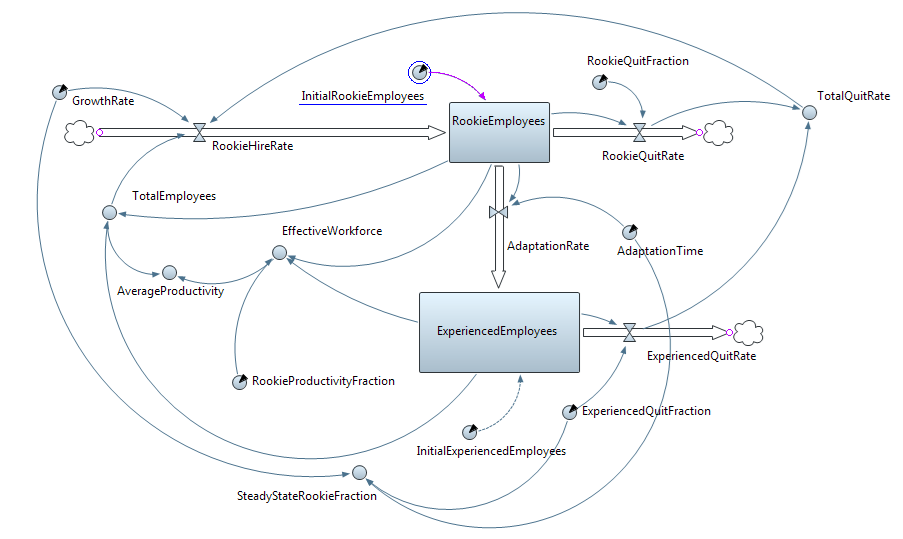
\includegraphics[width=0.8\textwidth]{icmon1}
	\caption{The cognitive map of the staff model.}
	\label{fig:icmon1}
\end{figure}  

The staff model consists of two stocks - Rookie Employees (Beginners) and Experienced Employees  and four flows:

\begin{itemize}
	\label{list:icmon1}
	\tightlist
	\item Rookie Hire Rate,
	\item Rookie Quit Rate,
	\item Adaptation Rate,
	\item Experienced Quit Rate.
\end{itemize}

Free parameters of the staff model are in te table \ref{tab:icmon1}: 

\begin{table}[H]
	\centering
	\caption{The free parameters of the staff model.}
	\label{tab:icmon1}
	\resizebox{\textwidth}{!}{%
		\begin{tabular} {|l|l|l| }
			\hline
			\textbf{Name} & \textbf{Description} & \textbf{Value} \\  \hline
			The speed of recruitment & Growth Rate & 0.01 per week ( from Total Employees) \\ \hline
			The initial number of newcomers to the company & Initial Rookie Employees & 40 people \\ \hline
			The initial number of experienced employees in the company & Initial Experienced Employees & 60 people \\ \hline
			The time of adaptation of the newcomer to the experienced employee & AdaptationTime & 50-100 weeks \\ \hline
			The percentage contribution of the novice in staff productivity & Rookie Productivity Fraction & 30-80\% \\ \hline
			The share of fired beginners & Rookie Quit Rate & 0.01 \\ \hline
			Share of layoffs of experienced employees & experienced Quit Fraction & 0.004 \\ \hline
		\end{tabular}
	}
\end{table}

Dynamic variables of the staff model are in table \ref{tab:icmon2}: 

\begin{table}[H]
	\centering
	\caption{The dynamic variables of the staff model.}
	\label{tab:icmon2}
	\resizebox{\textwidth}{!}{%
		\begin{tabular}{|l|l|}
			\hline
			\textbf{Variable name} & \textbf{Formula} \\ \hline
			Total Employees & RookieEmployees+ExperiencedEmployees \\ \hline
			Effective Workforce & ExperiencedEmployees + RookieProductivityFraction * RookieEmployees \\ \hline
			Average Productivity & EffectiveWorkforce / TotalEmployees \\ \hline
			Steady State Rookie Fraction & AdaptationTime*(ExperiencedQuitFraction+GrowthRate)/(1+AdaptationTime*(ExperiencedQuitFraction+GrowthRate)) \\ \hline
			Total Quit Rate & RookieQuitRate+ExperiencedQuitRate \\ \hline
		\end{tabular}%
	}
\end{table}

The flows listed in \ref{list:icmon1} calculated by the formulas from table \ref{tab:icmon3}:
 
\begin{table}[H]
	\centering
	\caption{The formulas for the staff model.}
	\label{tab:icmon3}
	\resizebox{\textwidth}{!}{%
		\begin{tabular}{|l|l|}
			\hline
			\textbf{Name of the flow} & \textbf{Formula} \\ \hline
			Rookie Hire Rate & RookieHireRate = TotalQuitRate + TotalEmployees*GrowthRate \\ \hline
			Rookie Quit Rate & RookieQuitRate = RookieEmployees*RookieQuitFraction \\ \hline
			Adaptation Rate & AdaptationRate = RookieEmployees/AdaptationTime \\ \hline
			Experienced Quit Rate & ExperiencedQuitRate = ExperiencedEmployees*ExperiencedQuitFraction \\ \hline
		\end{tabular}%
	}
\end{table}

The staff model produce the input for the task model to the simulation of the workload. 
The figure  \ref{fig:icmon2} shows the cognitive map of the task model, developed by the authors of this study.

\begin{figure}[ht]
	\centering
	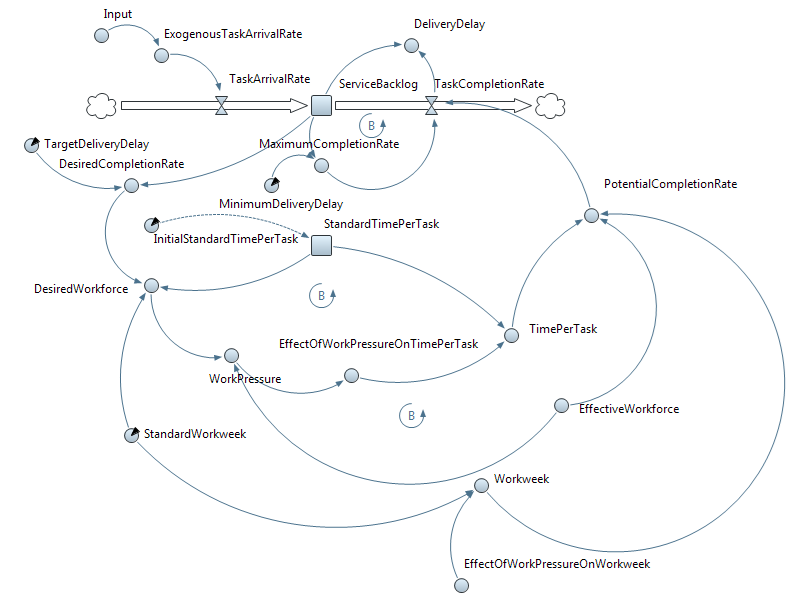
\includegraphics[width=0.8\textwidth]{icmon2}
	\caption{The cognitive map of the task model.}
	\label{fig:icmon2}
\end{figure}  

The task model consist of two stocks: ServiceBacklog (The task queue) and StandardTimePerTask (Standard time to complete the task). 
The table \ref{tab:icmon4} shows the free parameters that manage the task model:

\begin{table}[H]
	\centering
	\caption{The free parameters of the task model.}
	\label{tab:icmon4}
	\resizebox{0.5\textwidth}{!}{%
		\begin{tabular}{|l|l|}
			\hline
			\textbf{Parameter name} & \textbf{Parameter value} \\ \hline
			Standard Workweek & 40 hours \\ \hline
			Target Delivery Delay & 0.2 weeks \\ \hline
			Initial Standard Time Per Task & 1 person*hour/task \\ \hline
			Minimum Delivery Delay & 0.05 weeks \\ \hline
		\end{tabular}%
	}
\end{table}

The table \ref{tab:icmon5} shows the dynamic variables of the task model.
\begin{table}[H]
	\centering
	\caption{The dynamic variables of the task model.}
	\label{tab:icmon5}
	\resizebox{0.7\textwidth}{!}{%
		\begin{tabular}{|l|l|}
			\hline
			\textbf{Variable name} & \textbf{Formula} \\ \hline
			Desired Workforce & DesiredCompletionRate * StandardTimePerTask / StandardWorkweek \\ \hline
			Potential Completion Rate & EffectiveWorkforce * Workweek / TimePerTask \\ \hline
			Time Per Task & StandardTimePerTask * EffectOfWorkPressureOnTimePerTask(WorkPressure) \\ \hline
			Desired Completion Rate & ServiceBacklog / TargetDeliveryDelay \\ \hline
			WorkPressure & DesiredWorkforce / EffectiveWorkforce \\ \hline
			Workweek & StandardWorkweek * EffectOfWorkPressureOnWorkweek(WorkPressure) \\ \hline
		\end{tabular}%
	}
\end{table}

Exogenous dynamic flows of new jobs (TaskArrivalRate) and the flow of completed jobs (TaskCompletionRate) control the task queue (ServiceBacklog). 
The equation \ref{eq:icmon1} defines the equilibrium point for the task model.

\begin{equation}
EffectiveWorkforce = Desired Workforce
\label{eq:icmon1}
\end{equation}

The staff model and the task model coupled via dynamic variables. 
Together, these models represent the dynamics of skills and processes that characterize the intellectual capital of the organization, as we noted earlier.
The table \ref{tab:icmon6} shows the dynamic variables that couple two models.

\begin{table}[H]
	\centering
	\caption{The dynamic variables that couple the staff model and the task model.}
	\label{tab:icmon6}
	\resizebox{0.8\textwidth}{!}{%
		\begin{tabular}{|l|l|}
			\hline
			\textbf{Variable name} & \textbf{Action} \\ \hline
			Effective Workforce & Calculated in the staff model for the task model. Describes the number of employees for assignments. \\ \hline
			Workweek & Calculated in the task model for the staff model. Describes the number of hours required to complete incoming tasks. \\ \hline
		\end{tabular}%
	}
\end{table}

Lets examine the performance curves to identify the behavior of IC.  
The performance curve is a graphical representation of the change in learning rate of a particular activity. 
The figure \ref{fig:icmon3} shows the performance curves for the staff model for various values of time of adaptation of newcomers. 
In the staff model, the dynamic variable that characterizes productivity is Average Productivity variable.

\begin{figure}[H]
	\centering
	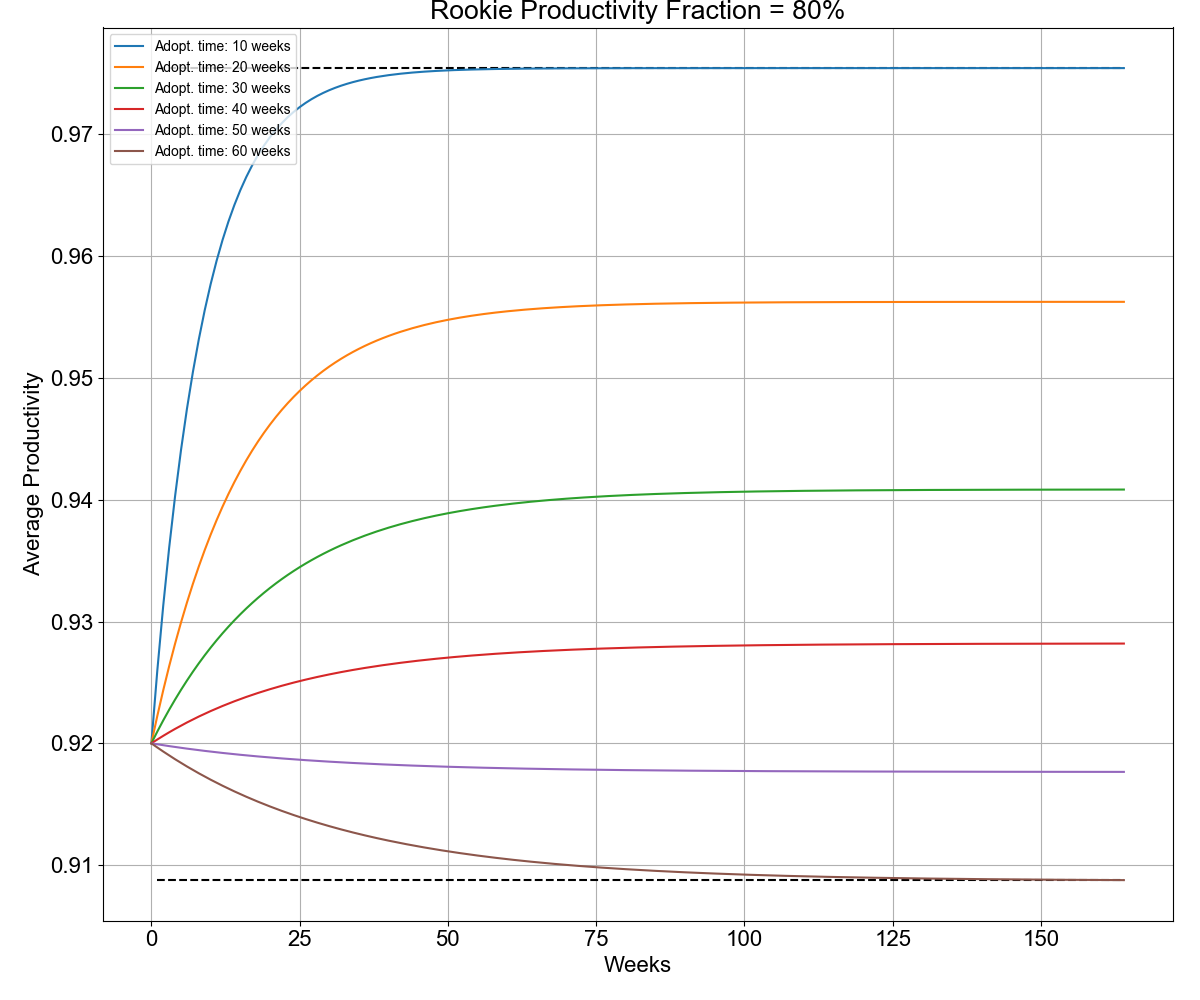
\includegraphics[width=0.8\textwidth]{icmon3}
	\caption{The performance curves for different AdaptationTime.}
	\label{fig:icmon3}
\end{figure}  

As we can see from the figure \ref{tab:icmon3} than Rookie Productivity Fraction is 80\%  and Adaptation Time is more than 50 weeks the learning curve goes to the lower asymptote, and at Adaptation Times over 60 weeks, the learning curve strives to the upper asymptote of the Average Productivity.
Consequently, demonstrating a different nature of the performance behavior. 
In practice, this means that with a significant adaptation time of newcomers, organizational productivity falls, as the number of experienced employees in the team decreases regarding beginners, and the contribution to productivity from beginners is less than from experienced employees.
On the other hand, the curves in the figure \ref{fig:icmon4} shows that for the Adaptation Time equal to 20 weeks, the productivity curves have a uniform character and differ in the rate of reaching the limit value – asymptote.

\begin{figure}[ht]
	\centering
	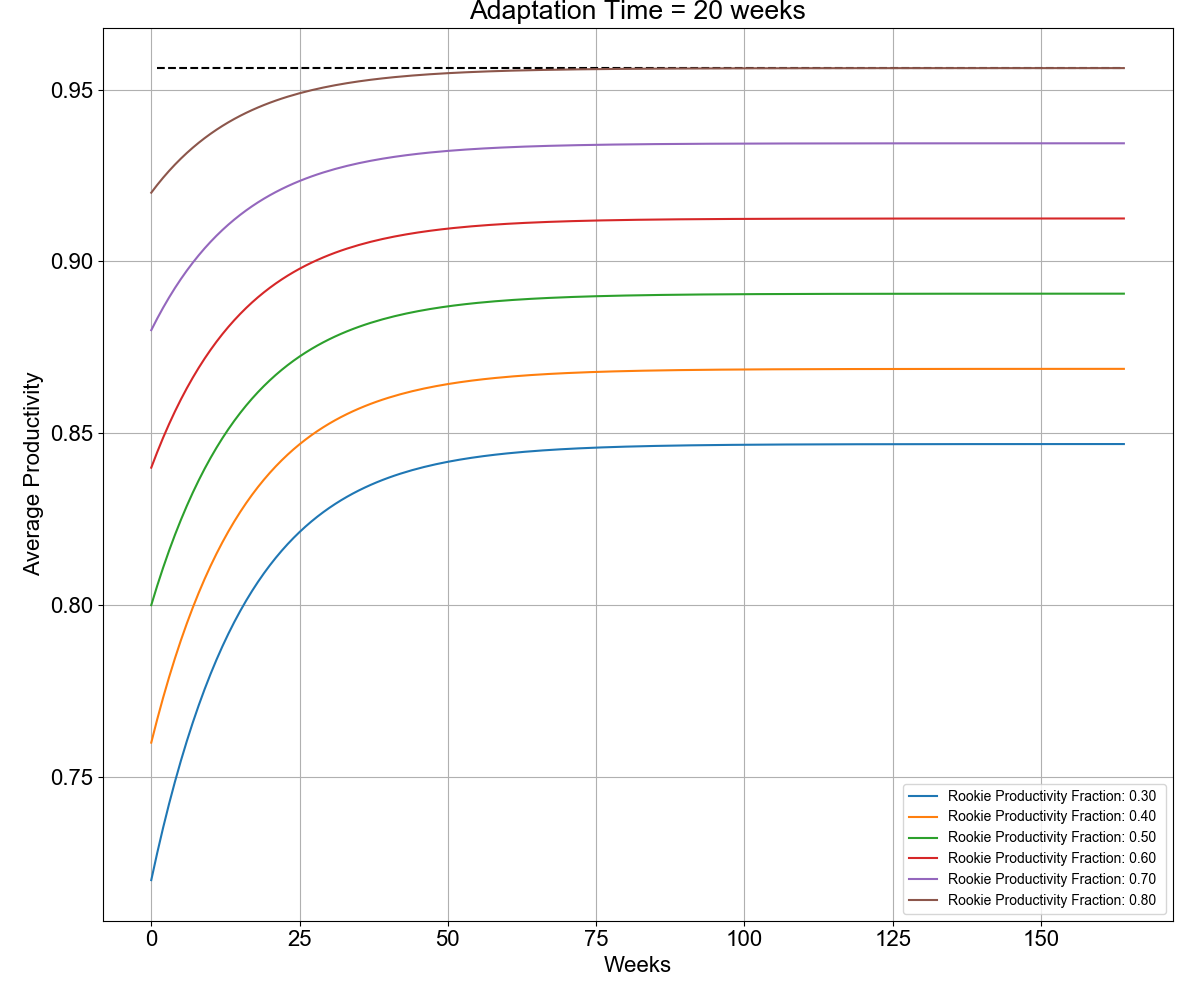
\includegraphics[width=0.8\textwidth]{icmon4}
	\caption{The performance curves for different Rookie Productivity Fractions.}
	\label{fig:icmon4}
\end{figure} 

The small contribution of newcomers means that the complexity of the tasks does not imply the participation of untrained staff. 
On the other hand, large proportions of newcomer contributions mean that assignments allow even an inexperienced staff member to work with high returns approaching the returns of experienced staff.

The exogenous function was used to simulate different regimes of workload on the task model.
The figure \ref{fig:icmon5} shows the performance for different regimes.

\begin{figure}[ht]
	\centering
	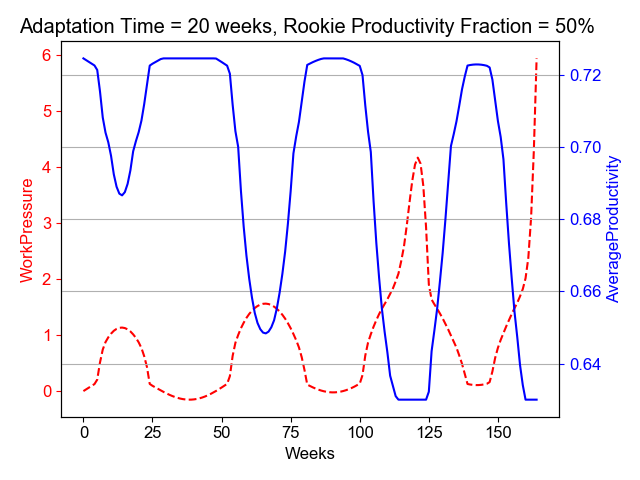
\includegraphics[width=0.8\textwidth]{icmon5}
	\caption{The performance and Work Pressure curves for the IC model.}
	\label{fig:icmon5}
\end{figure} 

From the figure \ref{fig:icmon5} we can see that in peak pressures the performance falls, but due to the adaptation of newcomers, the organization restores performance when the load falls. 
For different Adaptation Times in the IC model, the performance curves will have the form shown in the figure  \ref{fig:icmon6}.

\begin{figure}[ht]
	\centering
	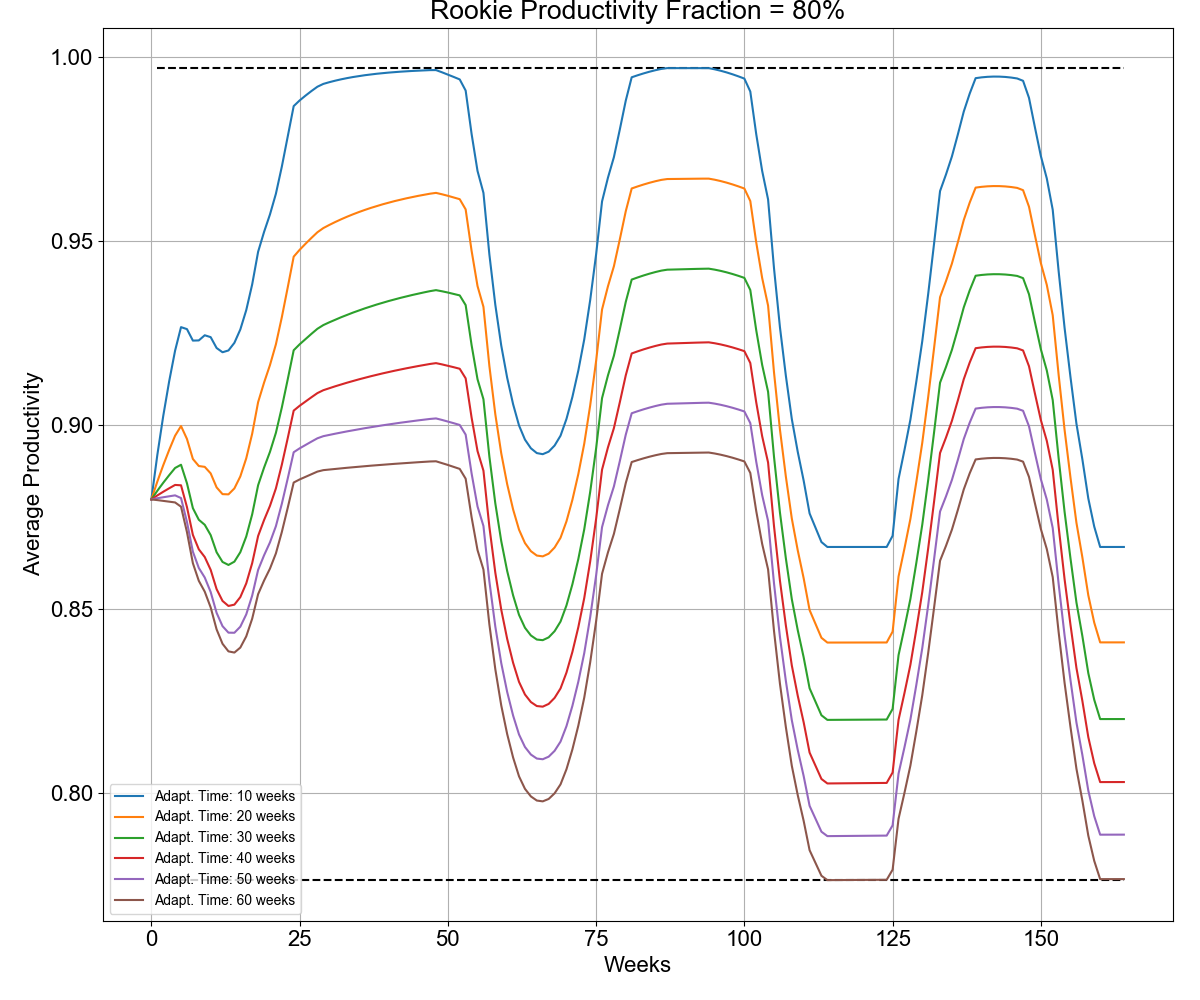
\includegraphics[width=0.8\textwidth]{icmon6}
	\label{fig:icmon6}
	\caption{The performance curves for the IC model with different Adaptation Times.}
\end{figure}

The figure \ref{fig:icmon7} presents performance curves for an adaptation Time of 20 weeks, taking into account the load.
We can observe different performance behavior before entering the asymptotes with different shares of newcomers, which reflects the fact that the possible inclusion of newcomers in the solution of tasks (before adaptation) characterizes these tasks as quite typical and straightforward.

\begin{figure}[H]
	\centering
	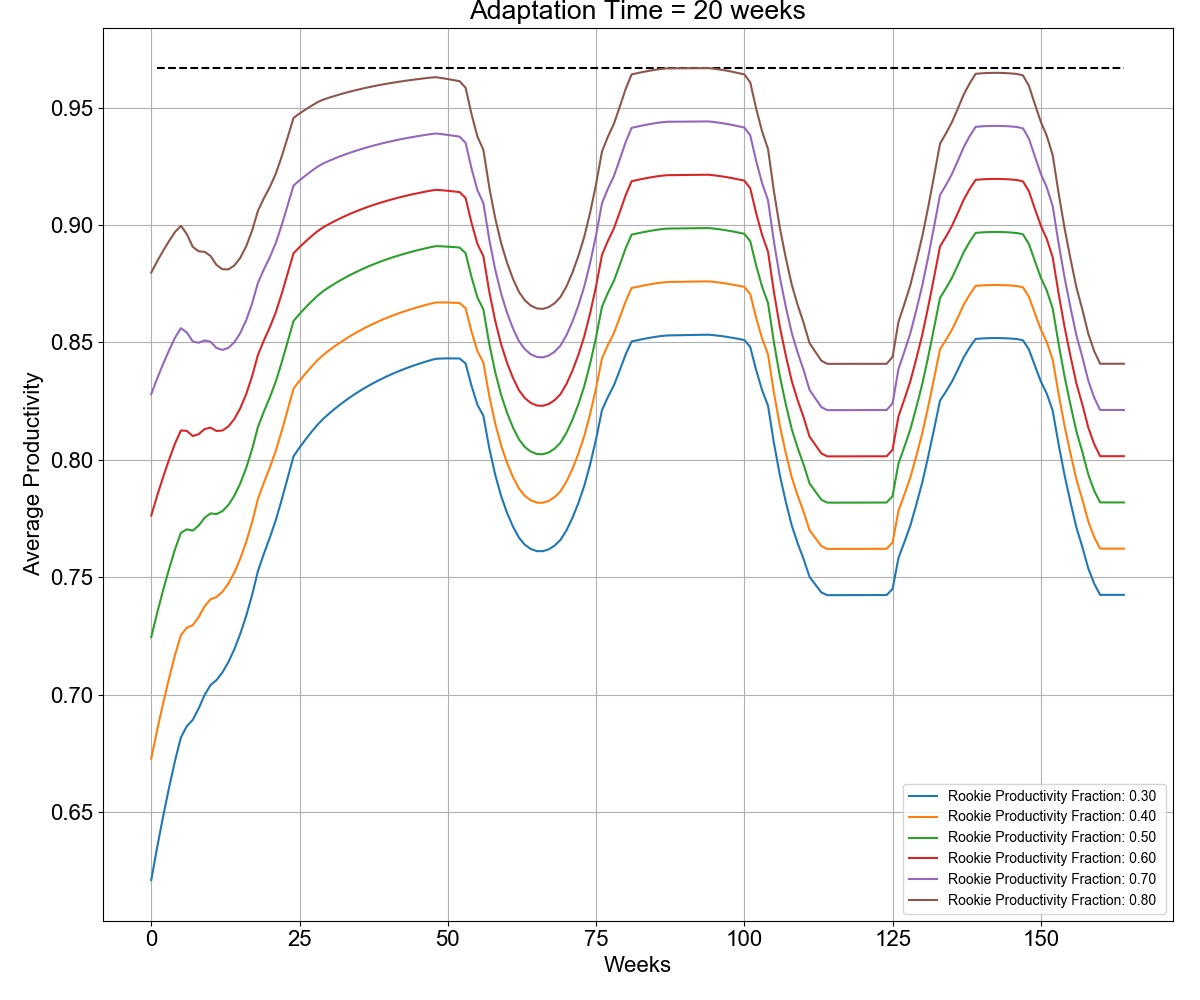
\includegraphics[width=0.8\textwidth]{icmon7}
	\caption{The performance curves for different Rookie Productivity Fractions with pressure.}
	\label{fig:icmon7}
\end{figure} 

Note that with a short adaptation time of beginners (20 weeks) and a high share of newcomers in productivity (80\%), the relative decline in productivity is lower than with a low high share of newcomers in productivity (30\%). 
This observation confirms the fact that with the increasing pressure of short and simple tasks for beginners their productivity falls less than on complex tasks.

To simulate the effect of burnout and fatigue of employees in the conditions of long-term work in the mode of the extended week, the following dependencies are introduced in the IC model:

\begin{enumerate}
	\tightlist
	\item The effect of burnout is to increase the rate of dismissal of experienced employees, depending on the time of work in an extended week.
	\item The effect of fatigue of employees is to reduce the productivity of employees depending on the time of work in an extended week.
\end{enumerate}

The figure \ref{fig:icmon8} shows the result of simulation of the IC model for 500 weeks. 
Such a long-term is chosen to show the effects of burnout and fatigue of the staff and as a consequence the decline in productivity caused by work in the extended working week.

\begin{figure}[ht]
	\centering
	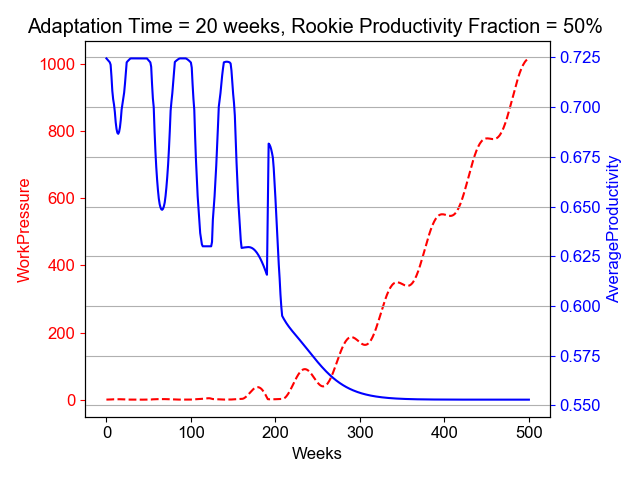
\includegraphics[width=0.8\textwidth]{icmon8}
	\caption{The performance curves and pressure for the IC model with the extended working week.}
	\label{fig:icmon8}
\end{figure} 

The performance drop caused by prolonged high load has a dramatic effect on the IC. 
In conclusion, the figure \ref{fig:icmon9} shows the curves of changes in human capital -- experienced employees, beginners and the total number of employees.  The curve of the required number of employees to perform incoming tasks is shown separately. 
We see that the number of newcomers is growing faster than the number of experienced employees.

\begin{figure}[ht]
	\centering
	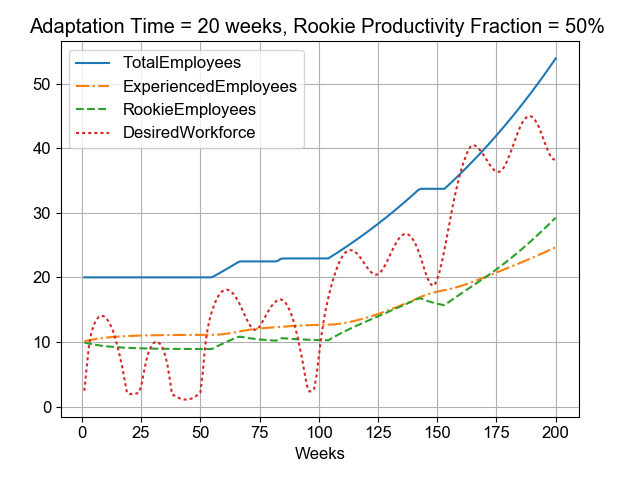
\includegraphics[width=0.8\textwidth]{icmon9}
	\caption{The curves of changes in human capital.}
	\label{fig:icmon9}
\end{figure} 

The results of the experiment confirm the theoretical work on the study of the processes of intellectual capital management. 
The novelty of this study is to develop quantitative assessments that help to clarify the strategy of the intellectual capital management research organization. 

The situation of workers in the conditions of high load considered by the author is typical for the Russian economy in modern conditions and is especially actual in oil and gas branch.

\section {The results of Team Building Modeling}
\label{sec:so}
For example, in industry research organization $\Omega$ laboratory work $\lambda_i$ , where $i \in (1 \dots N_{\lambda})$ . 
We denote the set of laboratories $ \Lambda = \{ \lambda_i, \dots, \lambda_{N_{\Lambda}} \}$.
The laboratories have researchers $ a = \{ a_{i}, \dots, a_{N_A} \} $.  
	
We denote the set of topics $t_i$, where $I \in (1, \dots, N_T )$, by which the organization $\Omega$ leads the R\&D as $T = \{ t_1, \dots , t_{N_T} \}$. Then the activities of the organization $\Omega$ to perform R\&D can be described by the following components (\ref{eq:so1}):

\begin{equation} 
\label{eq:so1}
\mathbb{M}_{\Omega} = \bigg \{ S, \Xi, \Psi, E \bigg \} \mbox {, where }  S = \{ \Lambda, A, T, P, X \}
\end{equation} 

In addition to the above defined components, there are in the \ref{eq:so1} equation:

\begin{itemize}
	\item $ \Xi = \{ \xi_1 , \dots , \xi_{N_{\Xi}} \} $ -- connections between the subjects (team work, co-authorship, etc.),
	\item $ \Psi = \{ \psi_1 , \dots , \psi_{N_{\Psi}} \} $ -- actions of the subjects  (theme search, call for papers, etc.),
	\item $ P = \{ \rho_1 , \dots , \rho_{N_P} \} $ -- researches,
	\item $ X = \{ \chi_1 , \dots , \chi_{N_X}  \} $ -- publishers.
\end{itemize}

Employees of the organization $\Omega$ perform research on topics $T$, create scientific articles and reports $P$ for publication in journals and presentations at conferences $X$.
When creating scientific articles $P$ reviews of journals and conferences $X$ are used.
Conferences and editorial offices of journals $X$ set priority topics $T$ and accept manuscripts for publication on a specific schedule (abstracts, full text, reviewers' comments, presentation, publication) and from the most qualified and experienced researchers.
The researcher has qualifications on the topics $T$, which can be represented as the $n$-dimensional vector $(c_1, \dots , c_{N_T} )$ and the experience of writing articles $(e_1 , \dots , e_{N_E} )$, where $c_i,e_i \in \mathbb{R}$. 
Both qualifications and experience do not need to be normalized. 
Qualification grows with the successful implementation of research, and experience grows with the successful publication of articles on relevant topics.

Simulation modeling is a statistical experiment. 
Its results should be based on relevant statistical tests. 
The author chose a repetition method to compute confidence intervals and test hypotheses.
Thus, each observation is presented as an independent run of the model, in which the transition period is not taken into account.
Then the average values of the sample are calculated. 
Since the runs are independent, a standard dispersion formula is applied.
The advantage of this method is that each simulation run of the model is determined by its sequence of random numbers from the interval $\left(0, 1\right)$, which provides statistical independence of the obtained observations. 
The disadvantage is that initial transient conditions can strongly influence all observations.

GazpromNeft STC was taken as calibration organization for modeling. 
Six research topics $T = \{ t_1, \dots , t_{N_T} \} $, where $N_T = 6 $, were chosen within the STC :
	
\begin{enumerate}
	\tightlist
	\item Development and exploitation of oil fields;
	\item Geology and exploration;
	\item Information technology in O\&G;
	\item Technologies of oil production;
	\item Design of the field construction;
	\item Drilling.	
\end{enumerate}	

As the publisher of $\chi_1$ selected edition of ``Oil industry'' produces the eponymous magazine since 1933. 
The authors chose the issue of the magazine for December 2016 (NX,12-2016), consisting entirely of articles by employees of Gazpromneft STC. 
The conference 16RPTC (SPE Russian Petroleum Technology Conference and Exhibition), held on October 24, 2016, in Moscow, was chosen as the conference $\chi_2$. 
Thus, $x = \{ \chi_1, \dots, \chi_{N_X}\}$, where $ N_{x} = 2$.

Currently, the analysis of social collaborations distinguishes two approaches:
\begin{itemize}
	\tightlist
	\item 
	The structural approach focuses on the geometric shape of the network and the intensity of interactions (edge weight). 
	In this case, Structural Theory and Network Exchange Theory are used to interpret the results;
	\item 
	The dynamic approach focuses on changes in network structure over time.
\end{itemize}

The experiment at this stage aimed to confirm the adequacy of the structure of the components of the model $\mathbb{M}_{\Omega}$ on the example of the scientific and technical center of the oil and gas industry. When observing the visualization of agent behavior, the authors did not need to add new components to the model.

For the set conditions from $\mathbb{M}_{\Omega}$ a private model $\mathbb{M}_{STC}$ was created and a lot of running simulation of the model was carried out.
One step of the simulation shown in the figure \ref{fig:so1}.
	
\begin{figure}[ht]
	\centering
	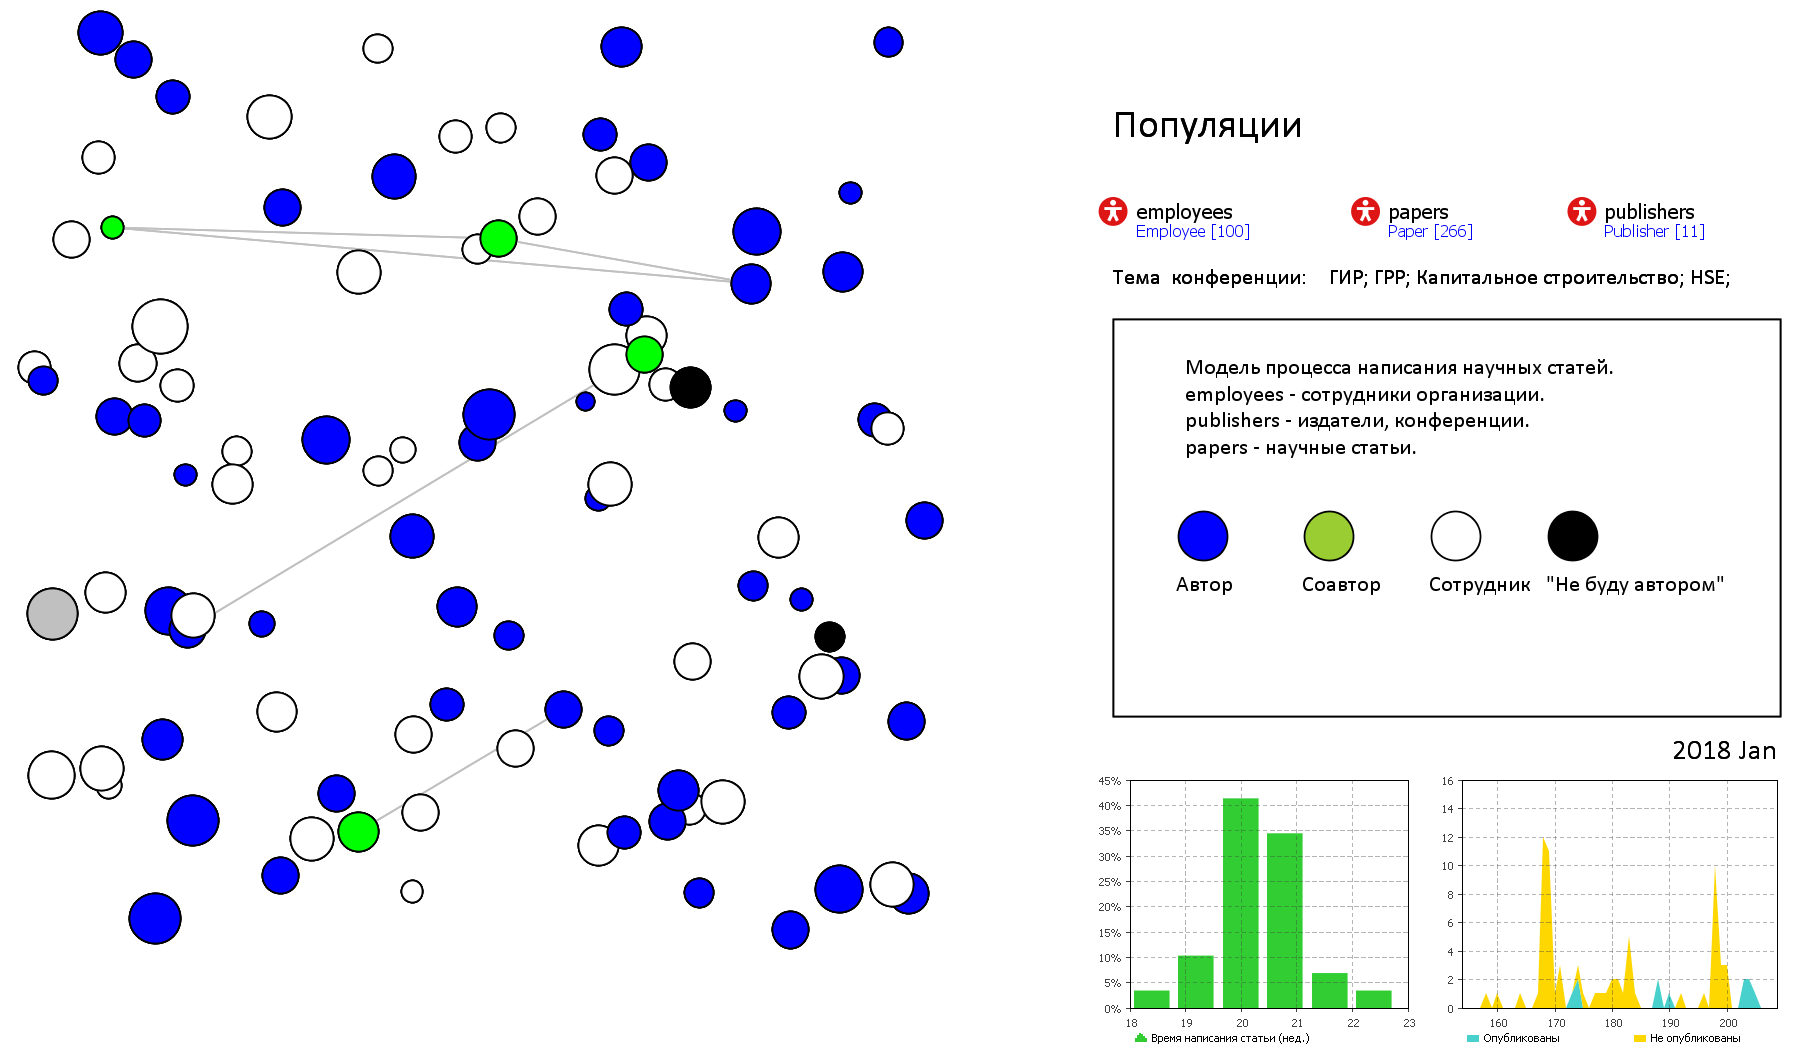
\includegraphics[width=0.9\textwidth]{so1}
	\caption{One step of the simulation.}
	\label{fig:so1}
\end{figure}

Moreover, by simulations, a database was created for the further study of the processes. 
The central database entities for the simulation of the $\mathbb{M}_{STC}$ model  are shown in the figure \ref{fig:so2}.  

\begin{figure}[ht]
	\centering
	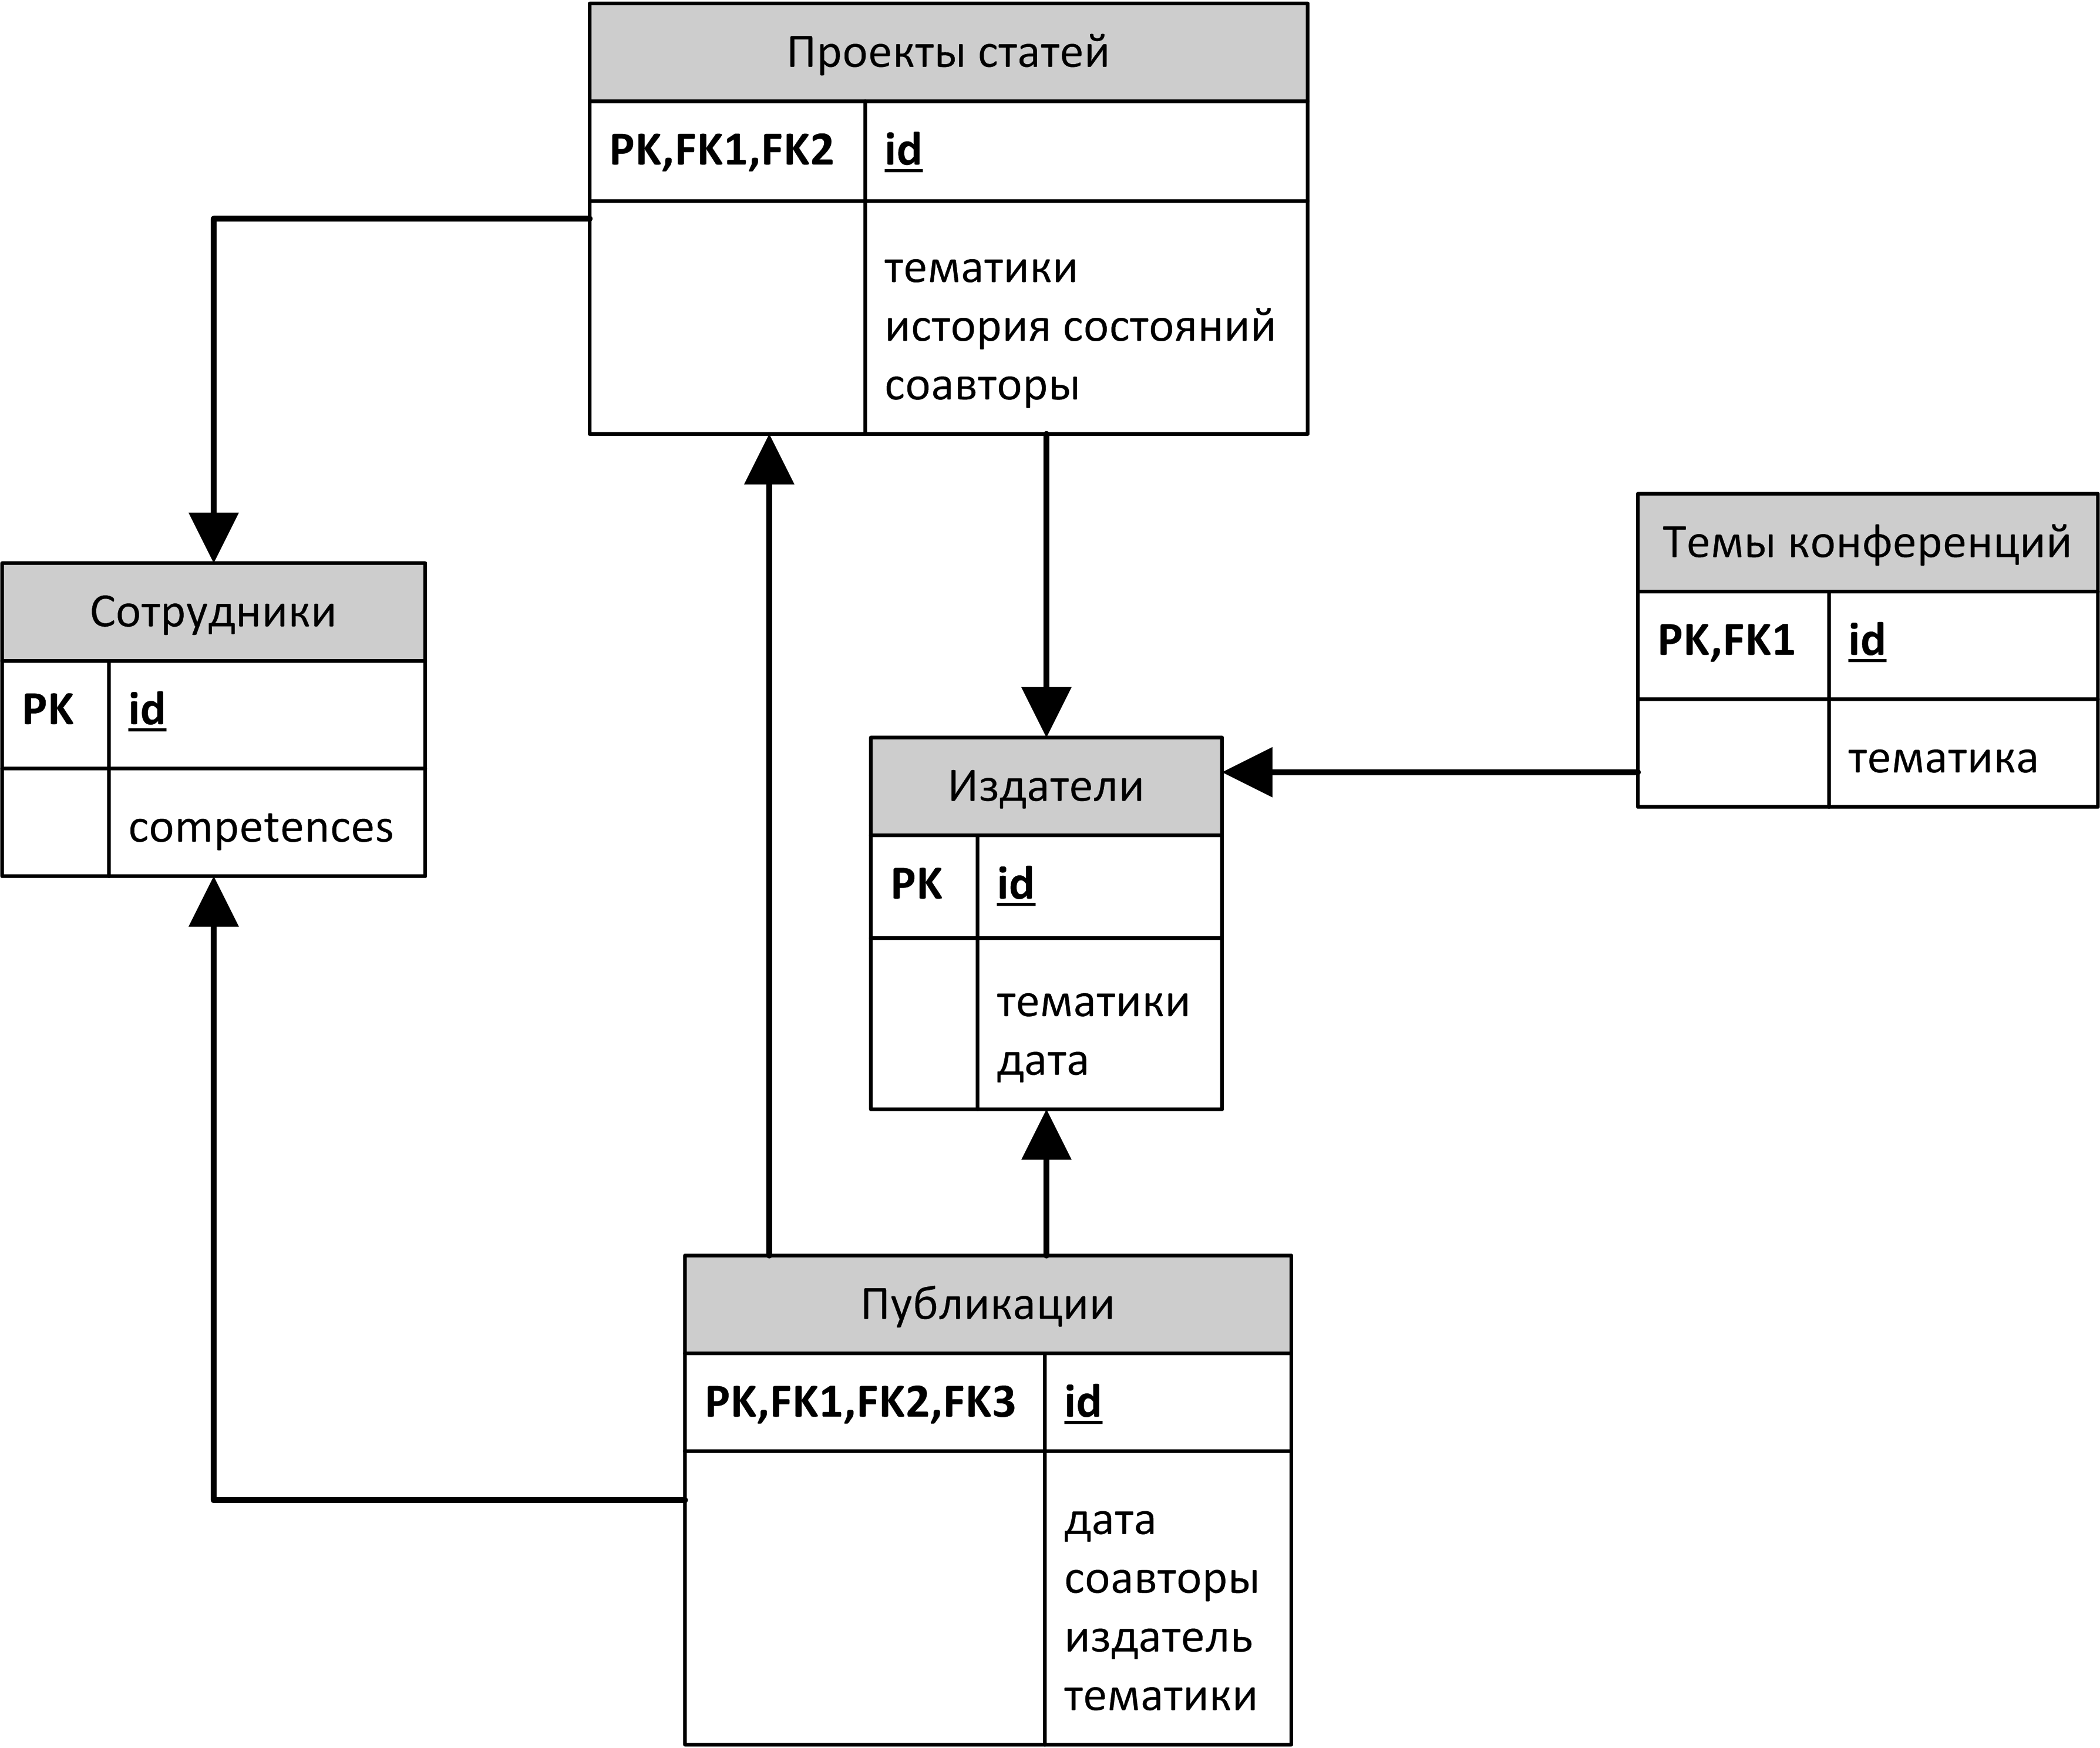
\includegraphics[width=0.6\textwidth]{so2}
	\caption{The ERD for the simulation of the $\mathbb{M}_{STC}$ model.}
	\label{fig:so2}
\end{figure}  

Based on the simulation results, we obtained the following results (\ref{tab:so1}) for the process of creating and publishing a scientific article.

\begin{table}[H]
	\centering
	\caption{The results of simulation of the $\mathbb{M}_{STC}$ model.}
	\label{tab:so1}
	\resizebox{0.7\textwidth}{!}{%
		\begin{tabular}{|l|l|}
			\hline
			\textbf{Variable name} & \textbf{Value} \\ \hline
			Average writing time & $20 \pm 2$ weeks \\ \hline
			Average number of co-authors & $3.5 \pm 1.0$ \\ \hline
			Maximum number of co-authors & $7 \pm 3$ \\ \hline
			Average number of articles per author per year & $2 \pm 0.5$ \\ \hline
			The share of articles that did not meet the publication schedule & $40 \pm 10$ \% \\ \hline
		\end{tabular}%
	}
\end{table}

The results are in agreement with the author's experience but need further verification.
A joint bibliometric study of real empirical data was carried out using the author's method \cite{KDGY} to assess the correctness of the simulation results. 
Under the conditions of the experiment, a database of publications containing the following information fields was created:

\begin{enumerate}
	\tightlist
	\item Publication date;
	\item Authors;
	\item Title;
	\item Key words according to the dictionary $T$;
	\item Publisher according to the list $X$.
\end{enumerate}


The database was consolidated from the articles of the publishing house ``Oil industry'' and publications from the electronic library of the community of oil and gas engineers SPE OnePetro.
The analysis of publications is carried out, and the graph of co-authors is constructed \ref{fig:so3}.

\begin{figure}[ht]
	\centering
	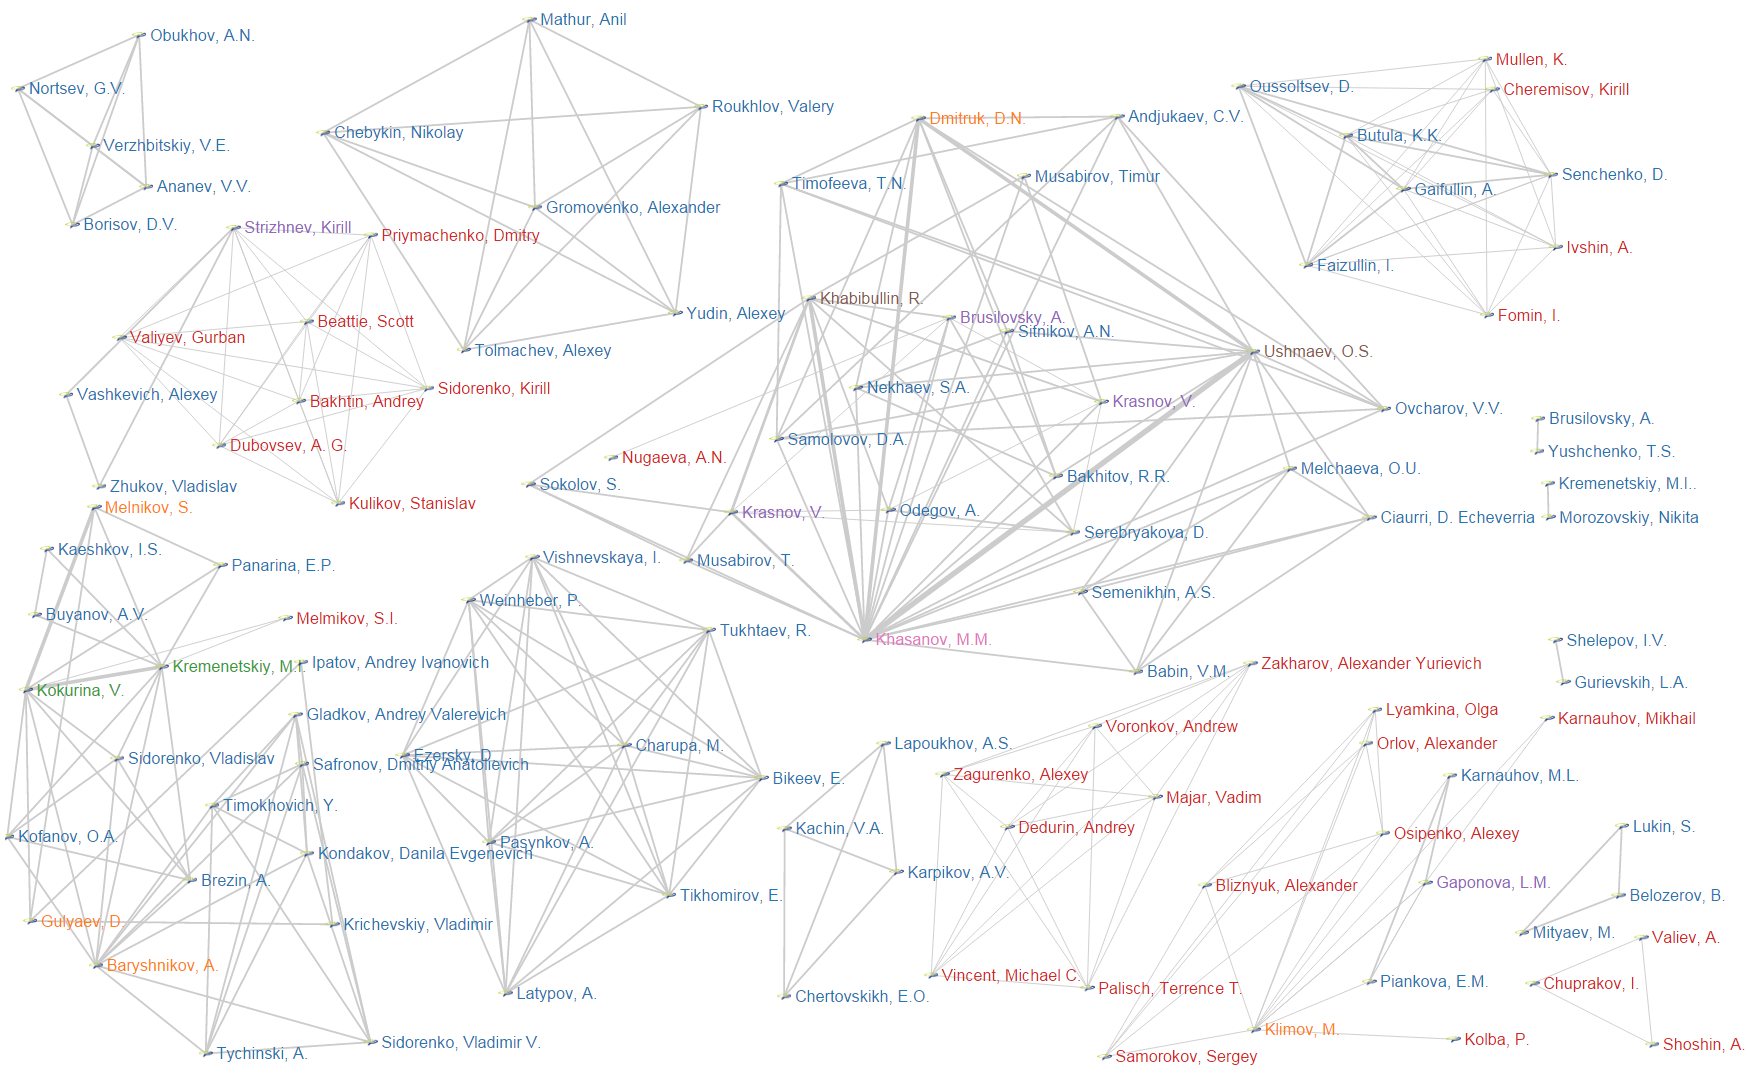
\includegraphics[width=0.8\textwidth]{so3}
	\caption{Co-authorship graph for Gazpromneft STC.}
	\label{fig:so3}
\end{figure}

Based on the database of publications, the following parameters of the collaboration are calculated (\ref{tab:so2}):

\begin{table}[H]
	\centering
	\caption{The results of the direct measurement of the STC activities.}
	\label{tab:so2}
	\resizebox{0.7\textwidth}{!}{%
		\begin{tabular}{|l|l|}
			\hline
			\textbf{Variable name} & \textbf{Value} \\ \hline
			Average number of published articles per author per year & $ 2 \pm 0.5$ \\ \hline
			Average number of co-authors & $2.8 \pm 0.1$ \\ \hline
			Maximum number of co-authors & $10 \pm 1$ \\ \hline
		\end{tabular}%
	}
\end{table}

The obtained empirical results confirm the results of the simulation, which indicates the prospects for the use of simulation as an analog for modeling social processes in an organizational environment.

\section{The result of optimization of the scientific activities}
\label{sec:scrum}
The task of finding the optimal parameters of the team of co-authors for the most productive contribution of scientific articles belongs to the class of optimization problems. 
The function that we want to minimize will depend on the following parameters:
\begin{itemize}
	\tightlist
	\item
	Number of employees in the organizational environment($N_{o}$);
	\item
	The rate of appearance of new employees ($Vemp_{new}$);
	\item
	The rate of staff quiting ($Vemp_{fired}$);
	\item
	Maximum number of employee competencies ($Cmax_{emp}$);
	\item
	The maximum number of competencies necessary to achieve the goal of the study ($Cmax_{pub}$).
\end{itemize}

The vector of the optimum values consists of the following variables:

\begin{itemize}
	\tightlist
	\item
	The time to publish a scientific article ($T_{pub}$);
	\item
	The fraction of employees who published articles ($Frac_{pub}$);
	\item
	The fraction of abandoned articles ($Frac_{notpub}$).
\end{itemize}

The following parameters represent the organization environment:

\begin{itemize}
	\tightlist
	\item
	Minimum and maximum number of employees in the organization	($N_{omax}$,$N_{omin}$);
	\item
	The rate of appearance of potential research targets ($V_{pub}$);
	\item
	Time limits for writing an article ($T_{eoc}$);
	\item
	Meeting speed ($V_{friending}$);
	\item
	The speed of a research target propagation ($V_{go}$)
\end{itemize}

Based on the above parameters, the cost function $\mathcal{F}$ for optimization can be written in the following form (\ref{eq:scrum5}).

\begin{equation} 
\label{eq:scrum5}
\mathcal{F}\bigg\{ \frac{1}{Frac_{pub}}, T_{pub}, Frac_{notpub} \bigg\} \rightarrow \, min
\end{equation}

The equation \ref{eq:scrum5} has the following constraints:
\begin{equation} 
\left\{ \begin{array}{rcl}
N_o \in [ N_{omin}, N_{omax} ]\\ 
Cmax_{emp} \leq Cmax_{pub} \in [ 1, N_{comp} ]\\
Vemp_{new} \geq Vemp_{fired} \geq 0
\end{array}\right.
\label{eq:scrum6}
\end{equation}

The optimization experiment was conducted in AnyLogic environment for two models: with and without Scrum.
Graphs of co-authorship stay the same. 
From the optimization experiment, the simulation of the co-authorship model developed by the author of this study was calibrated.
The optimal parameters $ N_{o} $, $ Vemp_{new} $, $ Vemp_{fired} $, $ Cmax_{emp} $, $ Cmax_{pub} $ were found for Gazpromneft STC.
The optimal values of the parameters are given in Table \ref{tab:ex1}.

\begin{table}[H]
	\caption{Optimal values of the scientific activities.}
	\label{tab:ex1}
	\centering
	\resizebox{0.9\textwidth}{!}{%
		\begin{tabular}{|l|c|}
			\hline
			\textbf{Name} & \textbf{Value} \\ \hline
			Number of employees in the organization ($N_o$) &  136 \\ \hline
			The rate of appearance of new employees ($Vemp_{new}$) & 1 per week \\ \hline
			Staff turnover ($Vemp_{fire}$) & 1 employee per month \\ \hline
			The maximum number of competencies of an employee ($Cmax_{emp}$) &  4 \\ \hline
			The maximum number of competencies necessary to achieve the goal of the study ($Cmax_{pub}$) & 5 \\ \hline
		\end{tabular}
	}
\end{table}

The calibrated model became the basis for the study of the effect of the introduction of Scrum roles in the process of writing scientific articles.
For the selected $T_{pub}$ and $Frac_{notpub}$ was carried out many simulation runs of two types: using the methods of Scrum and without Scrum. 
The data analysis was performed in the statistical environment $Python$.
The results of model runs  for $T_{pub}$ and $Frac_{notpub}$ shown in  figures \ref{ex:fig12} and \ref{ex:fig13} respectively.

\begin{figure}[ht]
	\centering
	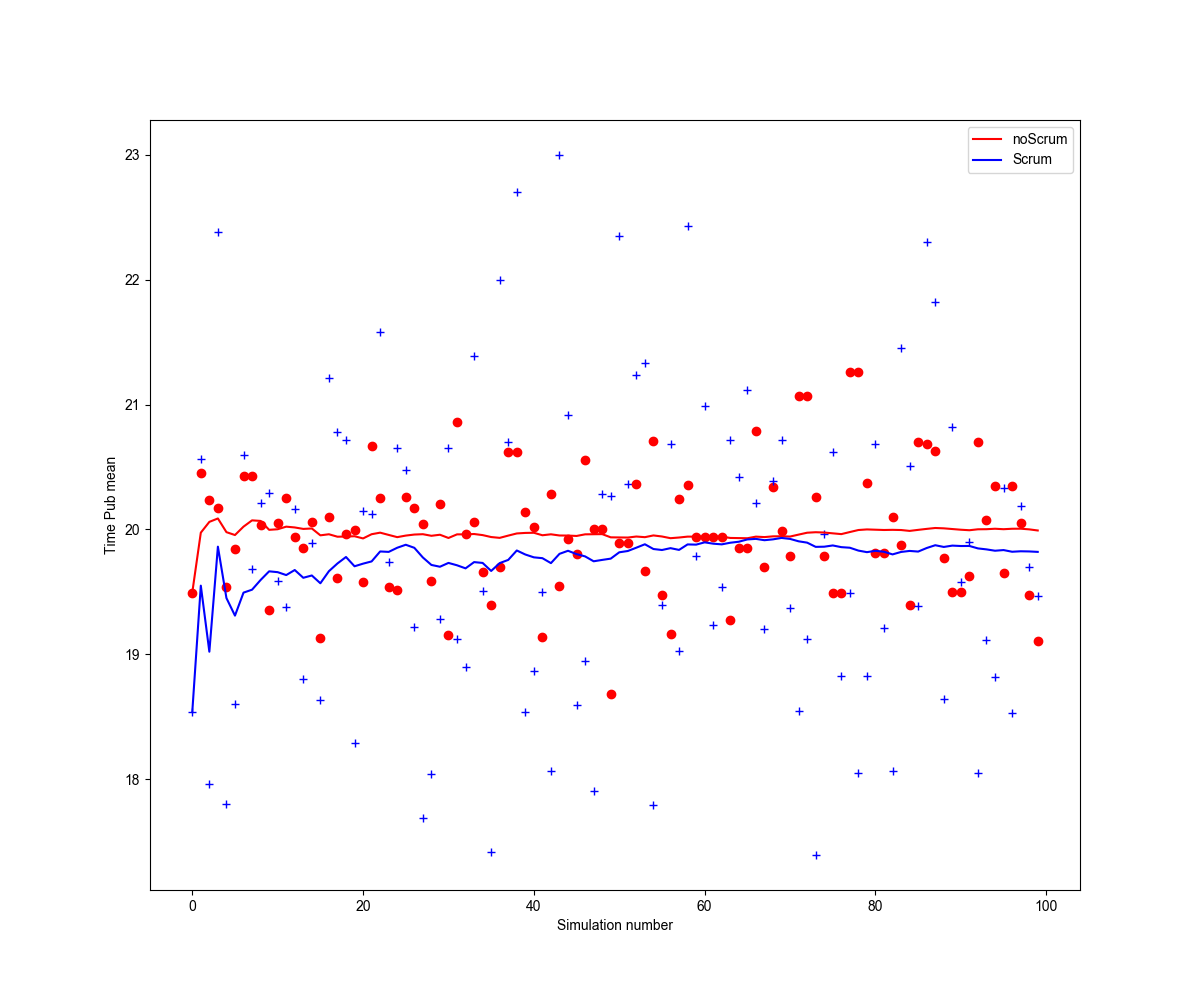
\includegraphics[width=0.8\textwidth]{scrum-img12}
	\caption{ The average time of publication of articles depending on the number of the run.}
	\label{ex:fig12}
\end{figure}  

\begin{figure}[ht]
	\centering
	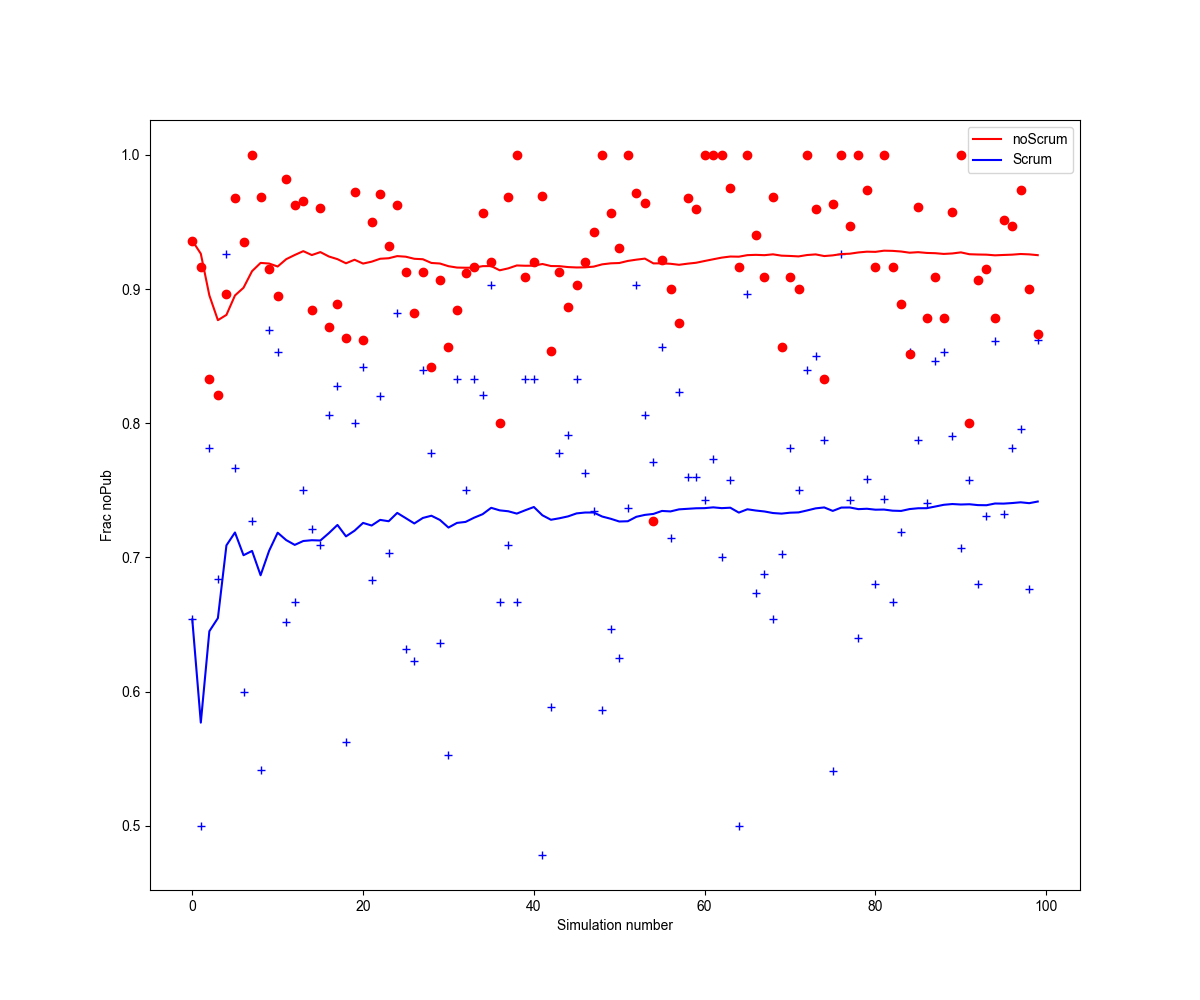
\includegraphics[width=0.8\textwidth]{scrum-img13}
	\caption{The share of abandoned scientific articles depending on the run number.}
	\label{ex:fig13}
\end{figure}  

In both figures, the lines show the dependence of the moving average.
To assess the impact of Scrum on the time of writing $T_{pub}$, the author compared the time of writing articles for two t-test samples to compare two independent samples.
The results showed that at the level of 1\% significance, the duration of writing articles using Scrum does not change.

\begin{itemize}
	\tightlist
	\item The average time to write a scientific article with Scrum was $19.90$ weeks with a standard deviation of $3.33$ weeks.	
	\item The average time to write a scientific article without Scrum was $19.90$ weeks with a standard deviation of $0.77$ weeks.
\end{itemize}

The author also additionally used the nonparametric Mann -- Whitney U-test in the case where the distribution of features does not correspond to the normal distribution, the results of which were similar to the t-test.
The results indicate that the use of Scrum does not accelerate the writing of articles, even if the function of writing articles is not subject to normal distribution.

Another indicator that can be used to measure Scrum productivity is the share of \textit{abandoned} scientific papers. 
We estimated the proportion of \textit{abandoned} scientific papers for teams that use Scrum and does not apply.

\begin{itemize}
	\tightlist
	\item
	The fraction of \textit{abandoned} scientific papers in the Scrum teams is $0.74$ with $\sigma =  0.02$;
	\item
	The fraction of \textit{abandoned} scientific papers in the non-Scrum teams is $0.92$ with $\sigma =  0.01$.
\end{itemize}

In other words, out of 100\% of the articles started in teams using Scrum, 26\% of the articles will be successful. 
In non-Scrum teams, only 8\% of articles will be in the time frame of the publication process with the required quality.

\section{Co-author Relationship Prediction}
\label{sec:allo}

Collective co-authorship in writing scientific articles has deterministic and random structural components. 
In addition to the rational aspects in the formation of a team of co-authors of a particular scientific article, there are emotional components. 
In the temporary perspective, working groups of researchers are formed and break up the labor collective, and the composition of contractors who participate in joint industry collaborations for research are updated.

Despite the complexity of co-authorship, there are several classes of models for simulating co-authorship. 
Among them are models based on random graphs and models of co-authorship formation based on co-author competencies. 
Both mathematical tools have been developed and used for several decades separately. 
However, there are not so many practical applications of co-authorship models in corporate practice.

The author hypothesized that it is necessary to combine several different types of models in order to better understand the nature of scientific collaborations in a separate organization. 

The author of this study set the task to develop a methodology for building a model of co-authorship for the scientific and technical center, taking into account the various structural components of co-authorship. 

As a result, the author has developed a model using machine learning methods, random graphs, and competency models. 
From the developed model the forecast of development of co-authorship in writing scientific articles of Gazpromneft STC is made.

The practical value of the results of this study is as follows: Quantified the contribution of various structural components in the formation of co-authors in writing scientific articles.

Forecasting the development of co-authorship in writing scientific articles allows to carry out 
planning corporate resources to support the growth of scientific publications.
Understanding the cluster structure of co-authorship allows aligning the areas of scientific activity under the strategic plan of the scientific and technical center.


Measurement of the activities of research organizations by the graph of co-authorship is a well-established practice. 
The researchers show opportunities to identify the highly productive authors and influential authors. 

The publication activity of  Gazpromneft STC was chosen as the object of research. 
The data were obtained from the onepetro open electronic library of the international community of petroleum engineers (SPE). 
After cleaning the data, 172 articles were left. 
The distribution of authors by year is shown in the figure \ref{fig:guest2}.

\begin{figure}[ht]
	\centering
	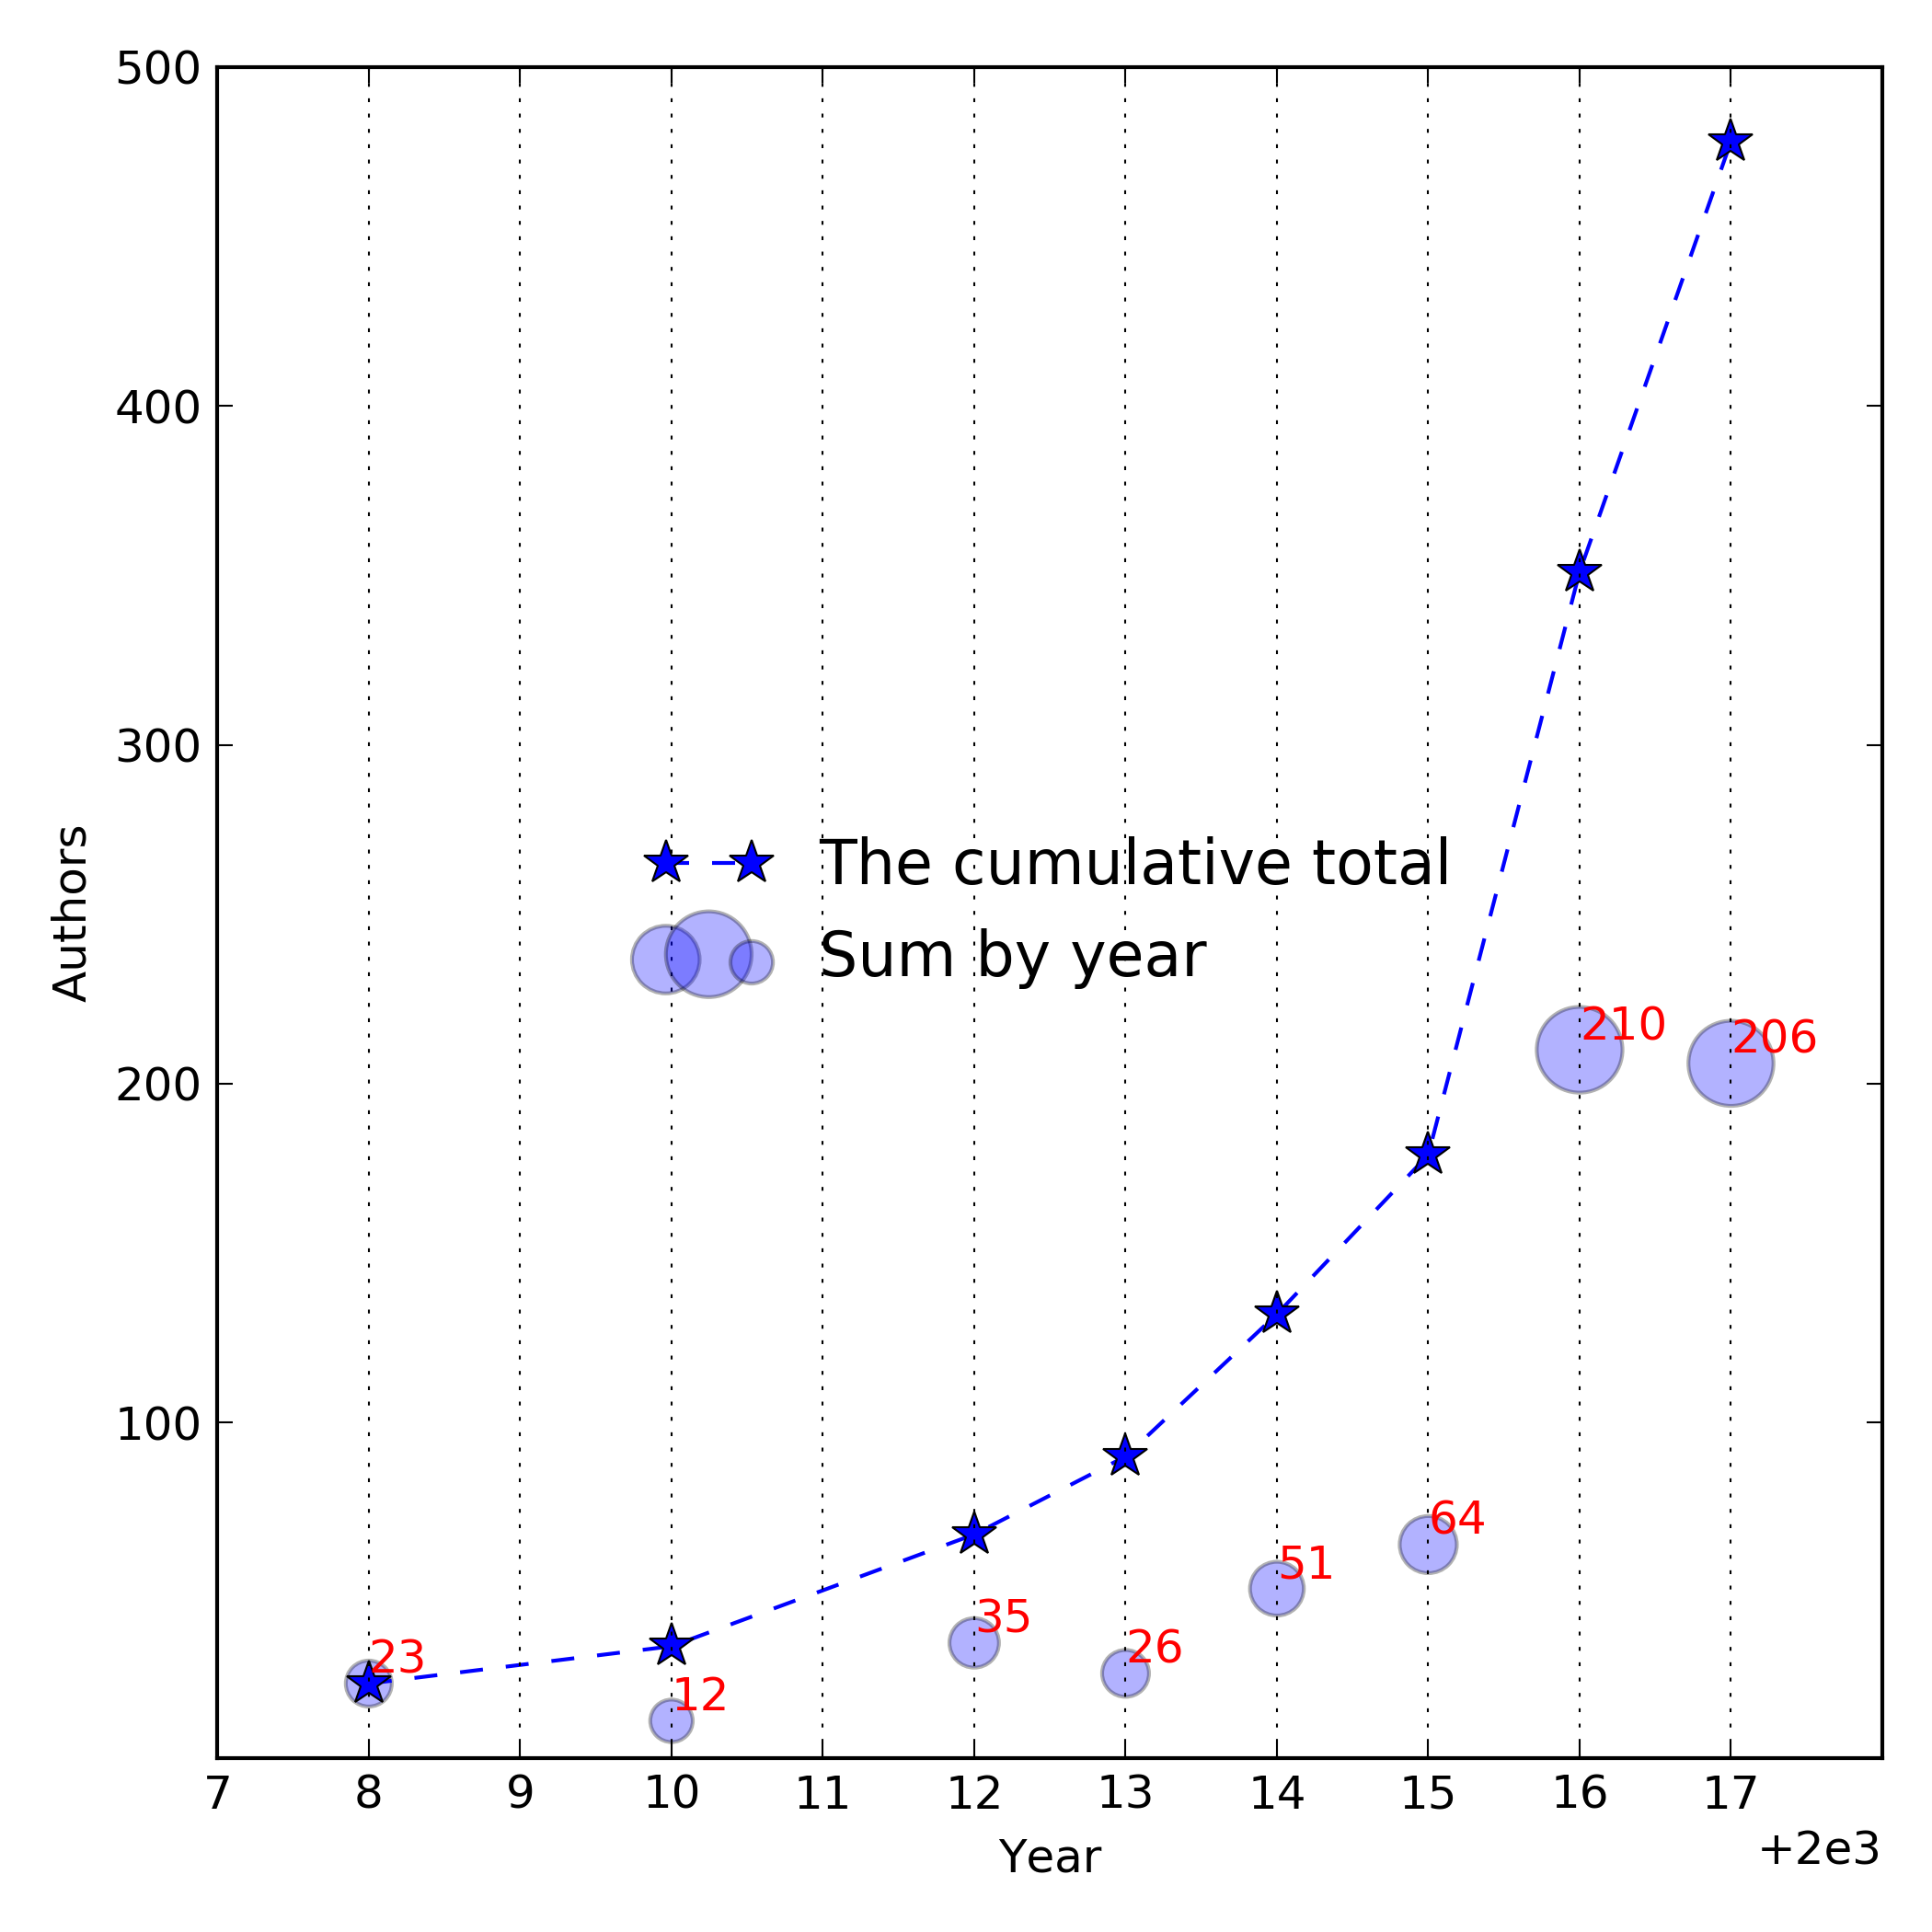
\includegraphics[width=0.8\textwidth]{guest2eng}
	\caption{Author allocation by year.}
	\label{fig:guest2}
\end{figure}  .

A direct answer to the placed research question can be an interpolation of the author quantity growth curve. We will receive the following dependency as a result of such assessment: with authenticity giving a forecast of 585 authors in 2018. On the graph, we can also see that the number of authors in 2017 (207) is less than in 2016 (210), which could be a growth saturation and influence the forecast.
Let us make a forecast based on the co-authorship graph. To do this, let us build a bipartite co-authorship graph \cite{krasnov2018bi} with node: author (479) and article (171). Authors possess technical competencies, while articles are characterized by their name, issue year and keywords. 

The obtained co-authorship graph has 26 connected components, the biggest of which contains 556 nodes, while the rest have no more than eight. Small connected components relate to authors that wrote their first article. The existence of small connected components can be looked at as one of the components for co-authorship graph growth. The Table \ref{tab:guest1} shows the quantity and size of connected components for each year with an accumulating total. 

% Please add the following required packages to your document preamble:
% \usepackage{booktabs}
\begin{table}[!ht]
	\centering
	\caption{The size of connected co-authorship graph components by year with an accumulating total.}
	\label{tab:guest1}
	\begin{tabular}{@{}|l|l|l|@{}}
		\toprule
		\textbf{Year} & \textbf{The size of connected components}                                                                                & \textbf{\begin{tabular}[c]{@{}l@{}}Small components\\ portion\end{tabular}} \\ \midrule
		2017          & \begin{tabular}[c]{@{}l@{}}\textbf{556}, 8, 8, 8, 6, 5, 5, 5, 4, 4,\\ 4, 4, 4, 4, 3, 3, 3, 2, 2, 2, 2, 2, 2, 2, 2, 2\end{tabular} & 15\%                                                                        \\ \midrule
		2016          & \begin{tabular}[c]{@{}l@{}}\textbf{367}, 8, 8, 8, 8, 8, 6, 5, 5, 5,\\ 5, 4, 4, 4, 4, 3, 3, 3, 2, 2, 2, 2, 2, 2, 2, 2\end{tabular} & 23\%                                                                        \\ \midrule
		2015          & \begin{tabular}[c]{@{}l@{}}\textbf{89}, 22, 21, 15, 12, 12, 8, 8, 8,\\ 8, 6, 6, 5, 4, 3, 3, 2, 2, 2, 2, 2\end{tabular}            & 63\%                                                                        \\ \midrule
		2014          & \begin{tabular}[c]{@{}l@{}}\textbf{46}, 18, 15, 12, 12, 10, 8, 8, 8,\\ 7, 6, 5, 4, 4, 3, 2, 2, 2, 2, 2\end{tabular}               & 74\%                                                                        \\ \midrule
		2013          & \begin{tabular}[c]{@{}l@{}}\textbf{23}, 15, 12, 11, 10, 8, 8, 7, 5,\\ 4, 4, 4, 2, 2, 2\end{tabular}                               & 80\%                                                                        \\ \midrule
		2012          & \textbf{15}, 14, 12, 11, 8, 8, 7, 4, 4, 4                                                                                         & 83\%                                                                        \\ \midrule
		2010          & \textbf{12}, 9, 8, 8, 4, 3                                                                                                        & 73\%                                                                        \\ \midrule
		2008          & \textbf{12}, 8, 7, 3                                                                                                              & 60\%                                                                        \\ \bottomrule
	\end{tabular}
\end{table}

Therefore, we can see that the co-authorship graph is progressing in quantity in the small connected components segment, while at the same time becoming more connected based on the number of nodes increasing in the main connected component. In order to increase the accuracy of forecasting it is expedient to take this structure into consideration. 

Incremental co-authorship graph growth dynamic by year is depicted in Figure \ref{fig:guest3}. We specify that the co-authorship graph of 2017 is the sum of all depicted in Figure \ref{fig:guest3}.

%\begin{figure}[!ht]
%	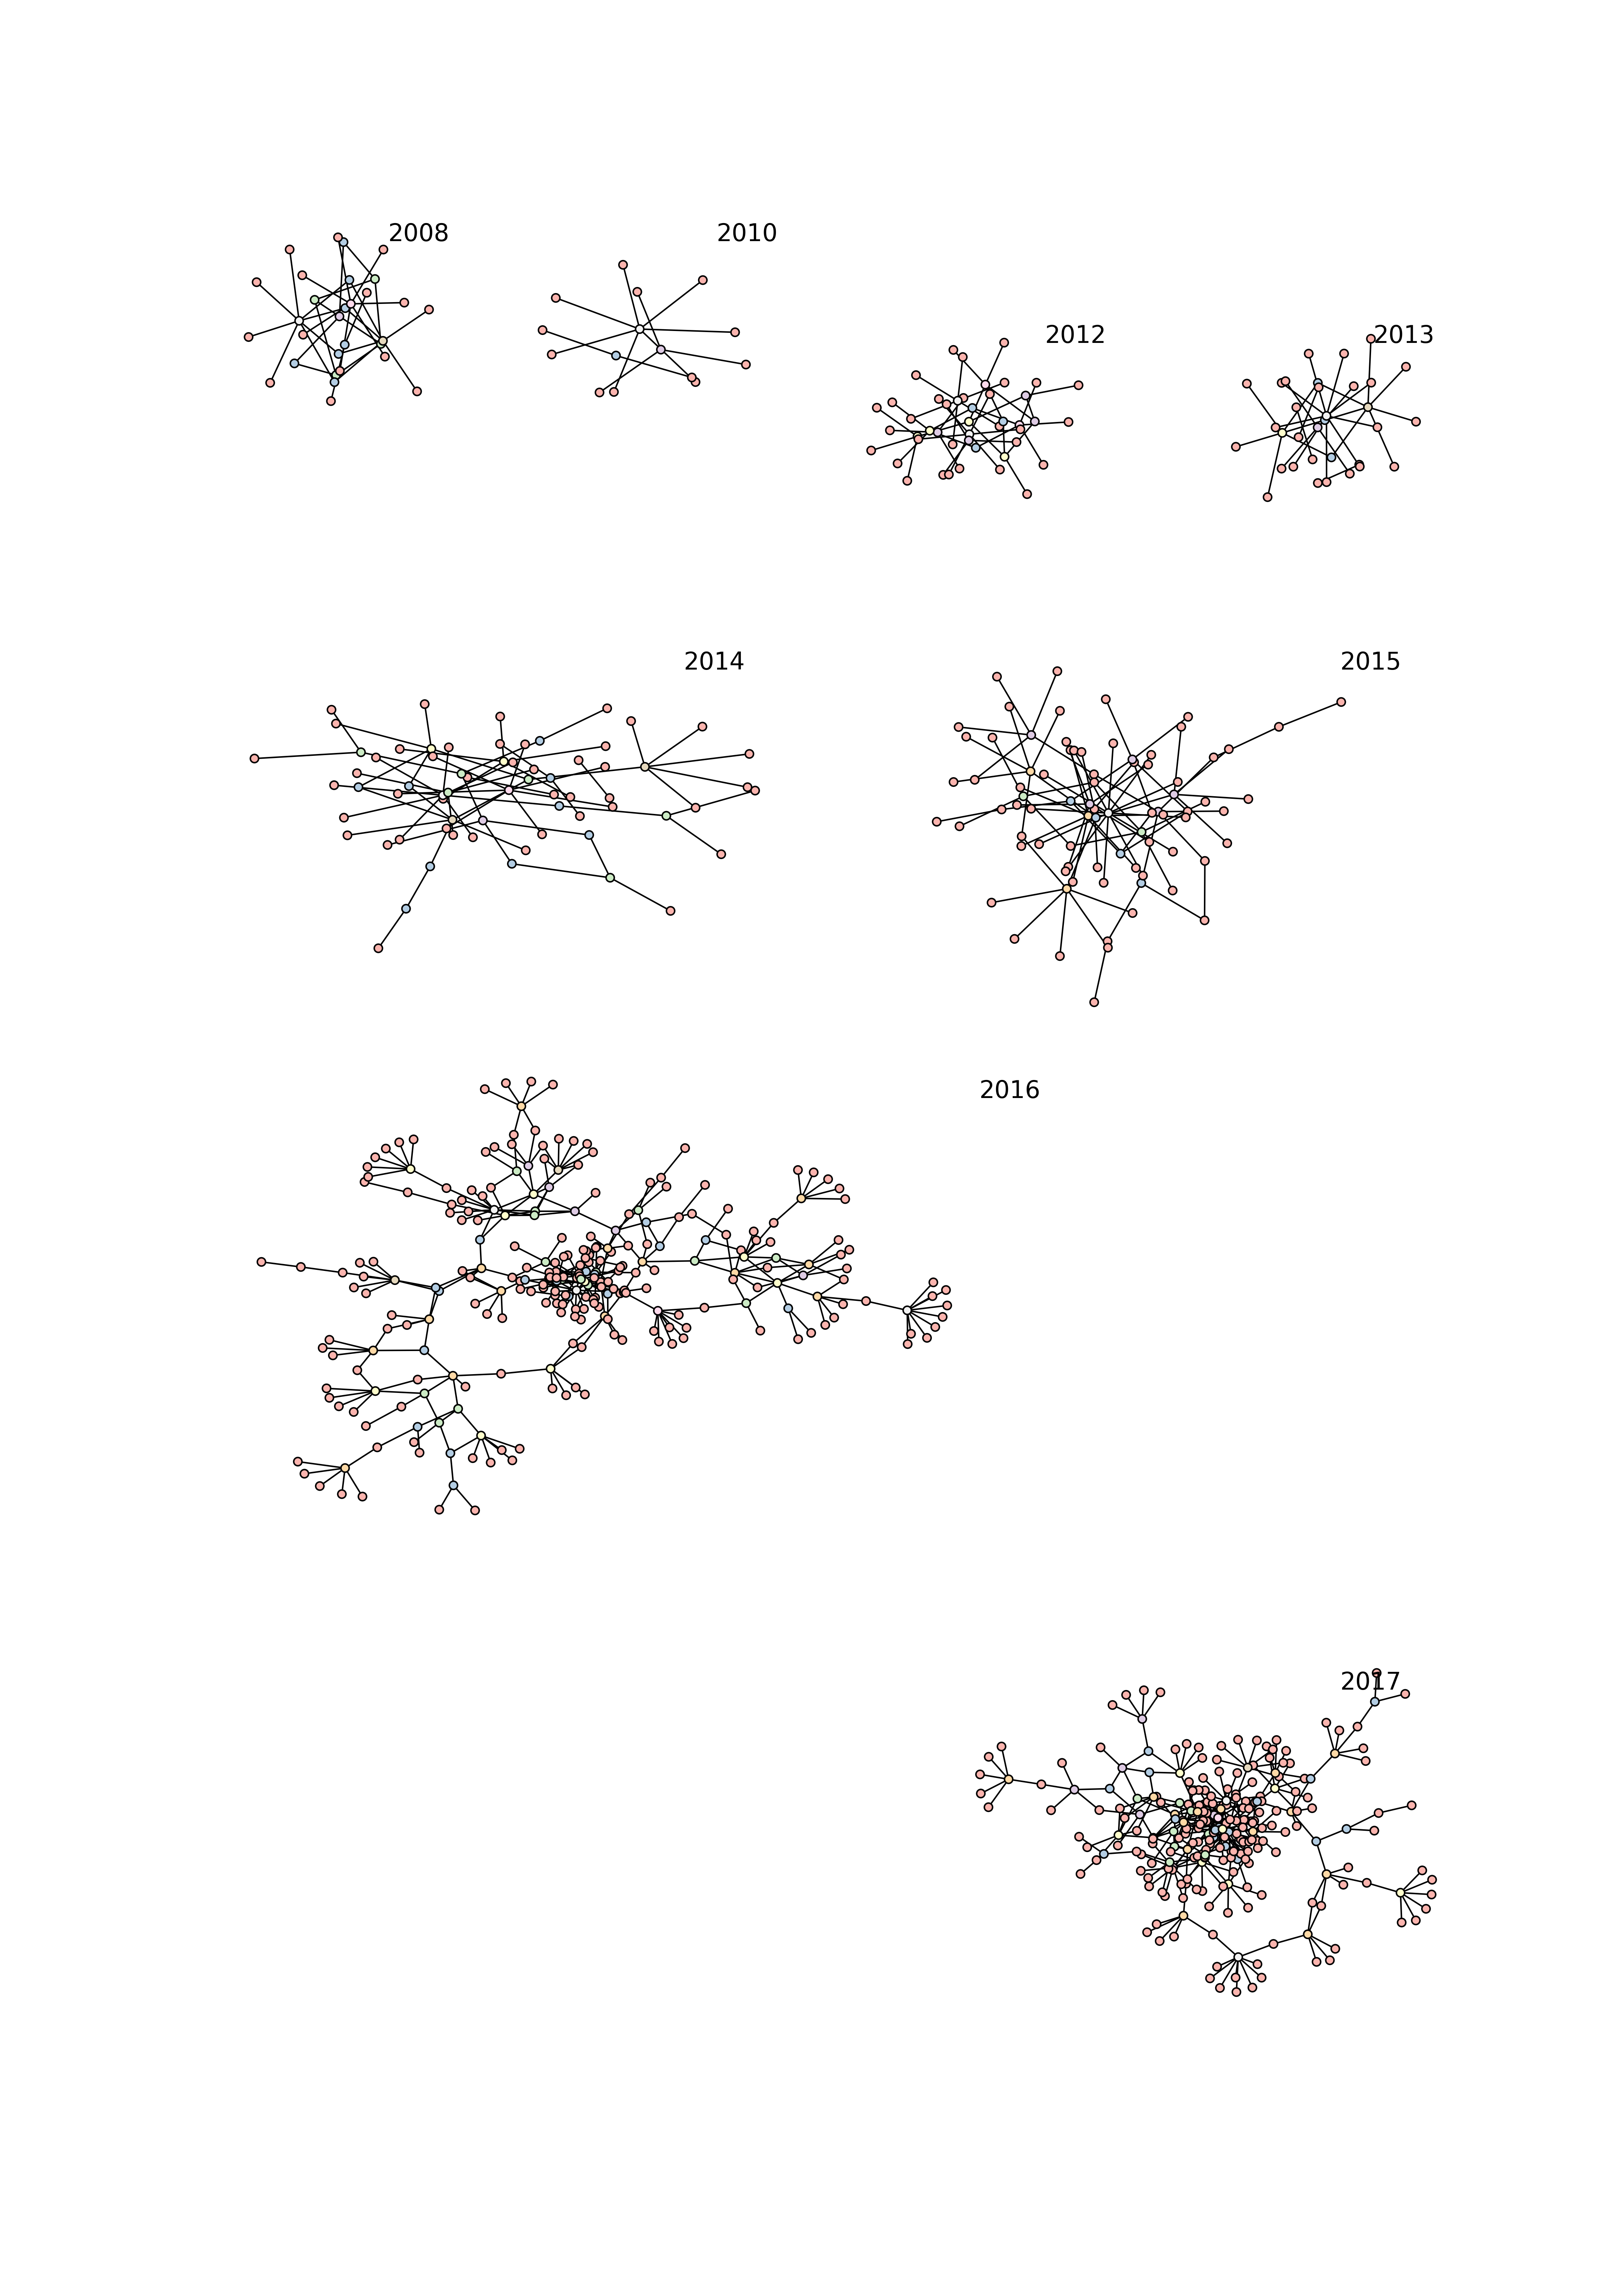
\includegraphics[width=\textwidth]{guest3eng.png}
%	\caption{The co-authorship development growth dynamic by year graph.}
%	\label{fig:guest3}
%\end{figure}

From the figure Figure \ref{fig:guest3} we can make a quality conclusion about the increase of quantity of annually added connections to the co-authorship graph. The change in growth leads to the co-authorship graph becoming more complex in 2016, which can be stated to be the ``elbow effect'' \cite{ketchen1996application}.

We will use the following graph node metrics in order to forecast authorship:

\begin{itemize}
	\tightlist
	\item Degree centrality
	\item Betweenness centrality
	\item Closeness centrality
	\item Harmonic centrality
	\item Clustering
\end{itemize}

The Figure \ref{fig:guest4} exposes the allocation of co-authorship graph node metrics.

\begin{figure}[ht]
	\centering
	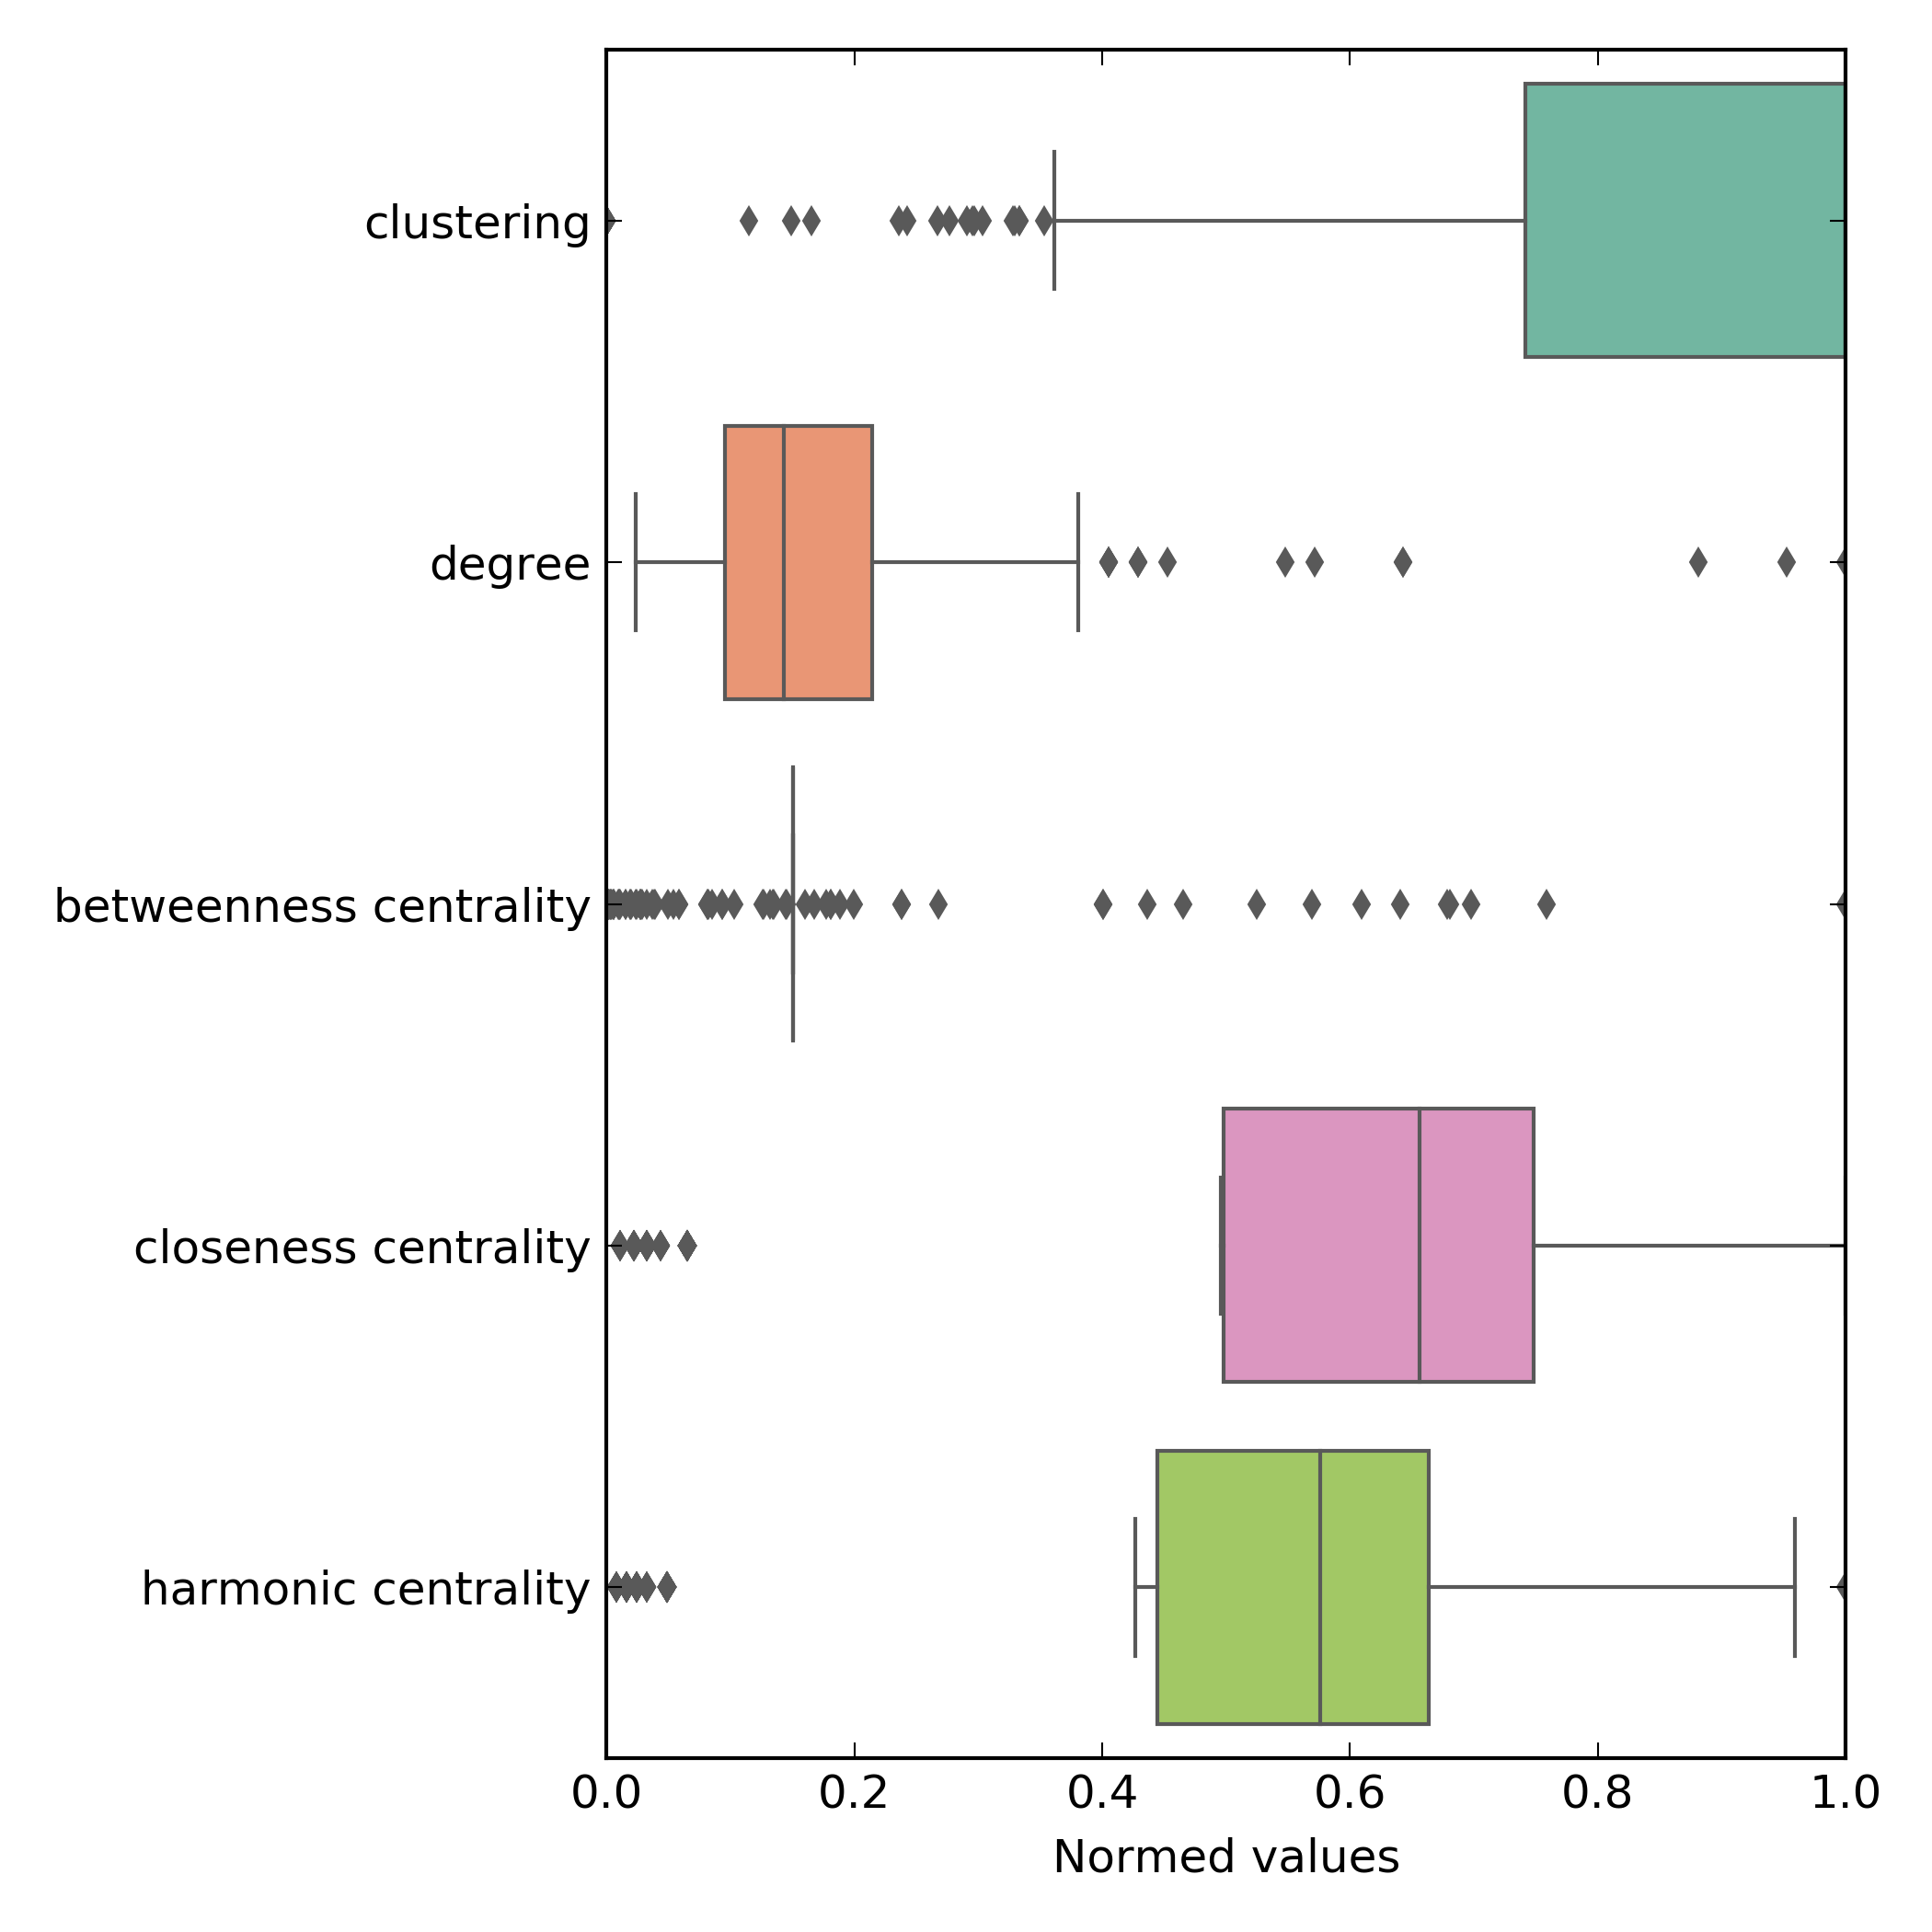
\includegraphics[width=0.7\textwidth]{guest4eng.png}
	\caption{Co-authorship graph node metrics.}
	\label{fig:guest4}
\end{figure}

We will use the binary classification model to forecast authorship. The model choice will be conducted based on the ROC-curve.  Model learning will be conducted with the 2016 metrics. Model parameters are optimized with the help of cross-validation with a 5-fold folding. The following results were obtained as a result of comparing different classifiers (Table \ref{tab:guest2}).

% Please add the following required packages to your document preamble:
% \usepackage{booktabs}
% \usepackage{graphicx}
\begin{table}[!ht]
	\centering
	\caption{Comparing classifier by the ROC AUC metric.}
	\label{tab:guest2}
	\begin{tabular}{@{}|l|l|@{}}
		\toprule
		Model                                                            & ROC-AUC \\ \midrule
		KNeighborsClassifier                                             & 0.66    \\ \midrule
		RidgeClassifier                                                  & 0.73    \\ \midrule
		RandomForestClassifier                                           & 0.72    \\ \midrule
		SVM                                                              & 0.70    \\ \midrule
		\begin{tabular}[c]{@{}l@{}}Multi-layer\\ perceptron\end{tabular} & 0.75    \\ \bottomrule
	\end{tabular}%
\end{table}

Multi-layer perceptron classifier based on a neural network with one layer consisting of 10 perceptions showed the best ROC AUC metric value.

The execution report of the authorship forecast for 2018 based on the co-authorship graph of 2017 is presented in the Table \ref{tab:guest3}.

% Please add the following required packages to your document preamble:
% \usepackage{booktabs}
% \usepackage{graphicx}
\begin{table}[!ht]
	\centering
	\caption{Classification report of authorship forecast for 2018.}
	\label{tab:guest3}
	%%\resizebox{\textwidth}{!}{%
	\begin{tabular}{@{}|l|l|l|l|l|@{}}
		\toprule
		Labels                                                & Precision & Recall & F1-score & Support \\ \midrule
		\begin{tabular}[c]{@{}l@{}}not\\ author\end{tabular}  & 0.80      & 0.98   & 0.88     & 66      \\ \midrule
		author                                                & 0.80      & 0.20   & 0.32     & 20      \\ \midrule
		\begin{tabular}[c]{@{}l@{}}Avg /\\ Total\end{tabular} & 0.80      & 0.80   & 0.75     & 86      \\ \bottomrule
	\end{tabular}%
	%%}
\end{table}

406 authors were predicted in 2018 as a result of forecasting. If we add employees who will write their first article in 2018 to the forecast, we will get an additional 15\% based on the assessment of the connected components growth dynamic. In total 467 employees will become authors in 2018.

\section{Results of Clustering of R\&D Trends}

Planning of research and development trends in science and technology centers should be in line with the actual state of things. Such phenomena as organizational frigidity, research diversification and propensity for developing IT products are able to significantly impair any strategies and development trends.   

However, feasibility of plans is an important attribute of development able to which significantly raise personnel’s motivation for achieving best results. This is why setting achievable goals is of such importance. 
There are never enough quantitative tools for appraisal of research and development activities. Formal paperwork reporting on STC is not suitable for evaluation of researchers’ involvement and dedication. 

Instead, small formats of research works such as presentations at scientific and technical conferences or scientific articles in peer-reviewed scientific publications require much more informal approach from researchers. Analysis of a science and technology center’s performance based on its publication activity is a common practice. Many studies analyze text corpus of scientific articles and make conclusions on development trends. Text data noise levels are quite high; even most advanced analysis methods based on word embedding are able to produce accurate predictions only if analyzed are huge text volumes which are seldom available in case of small organizations. Small research organizations suffer the most from inaccurate planning of research activities.

Author of this research propose to take advantages of articles (presentations) analysis based on co-authorship bipartite graph to extract research trends with the purpose of their further evaluation and planning.

From a formal point of view we have to solve the problem of unsupervised machine learning for co-authorship graph, attribute clusters to particular subjects and detect variations in clusters over the time.

Let us examine the conceptual meaning of the Betweenness centrality metrics applied to the problem of clustering of co-authorship graph in an STC. The Betweenness centrality metrics shows how important is a particular node for the graph’s connectivity. Connections in a co-authorship graph reflect research collaboration. Co-authorship graphs are not always connected; usually they consist of several connected components of various sizes. 

Connected components are natural clusters. Small connected components reflect primary initiatives – researchers’ first articles. However the main connected component may contain up to 90\% of a co authorship graph’s nodes and call for a special approach to clustering. 

To extract clusters from a main connected component of a co-authorship graph one may use the method of artificial removal of the nodes with the top-value Betweenness centrality metrics. As each of such nodes is removed a graph may break down into several disconnected components. The Figure \ref{fig:allo2} shows such separation model.  On the left side of the figure depicted initially connected graph. On the right side of the picture the same graph with the node with the top-value Betweenness centrality metrics removed looks like two connected components.

\begin{figure}[ht]
	\centering
	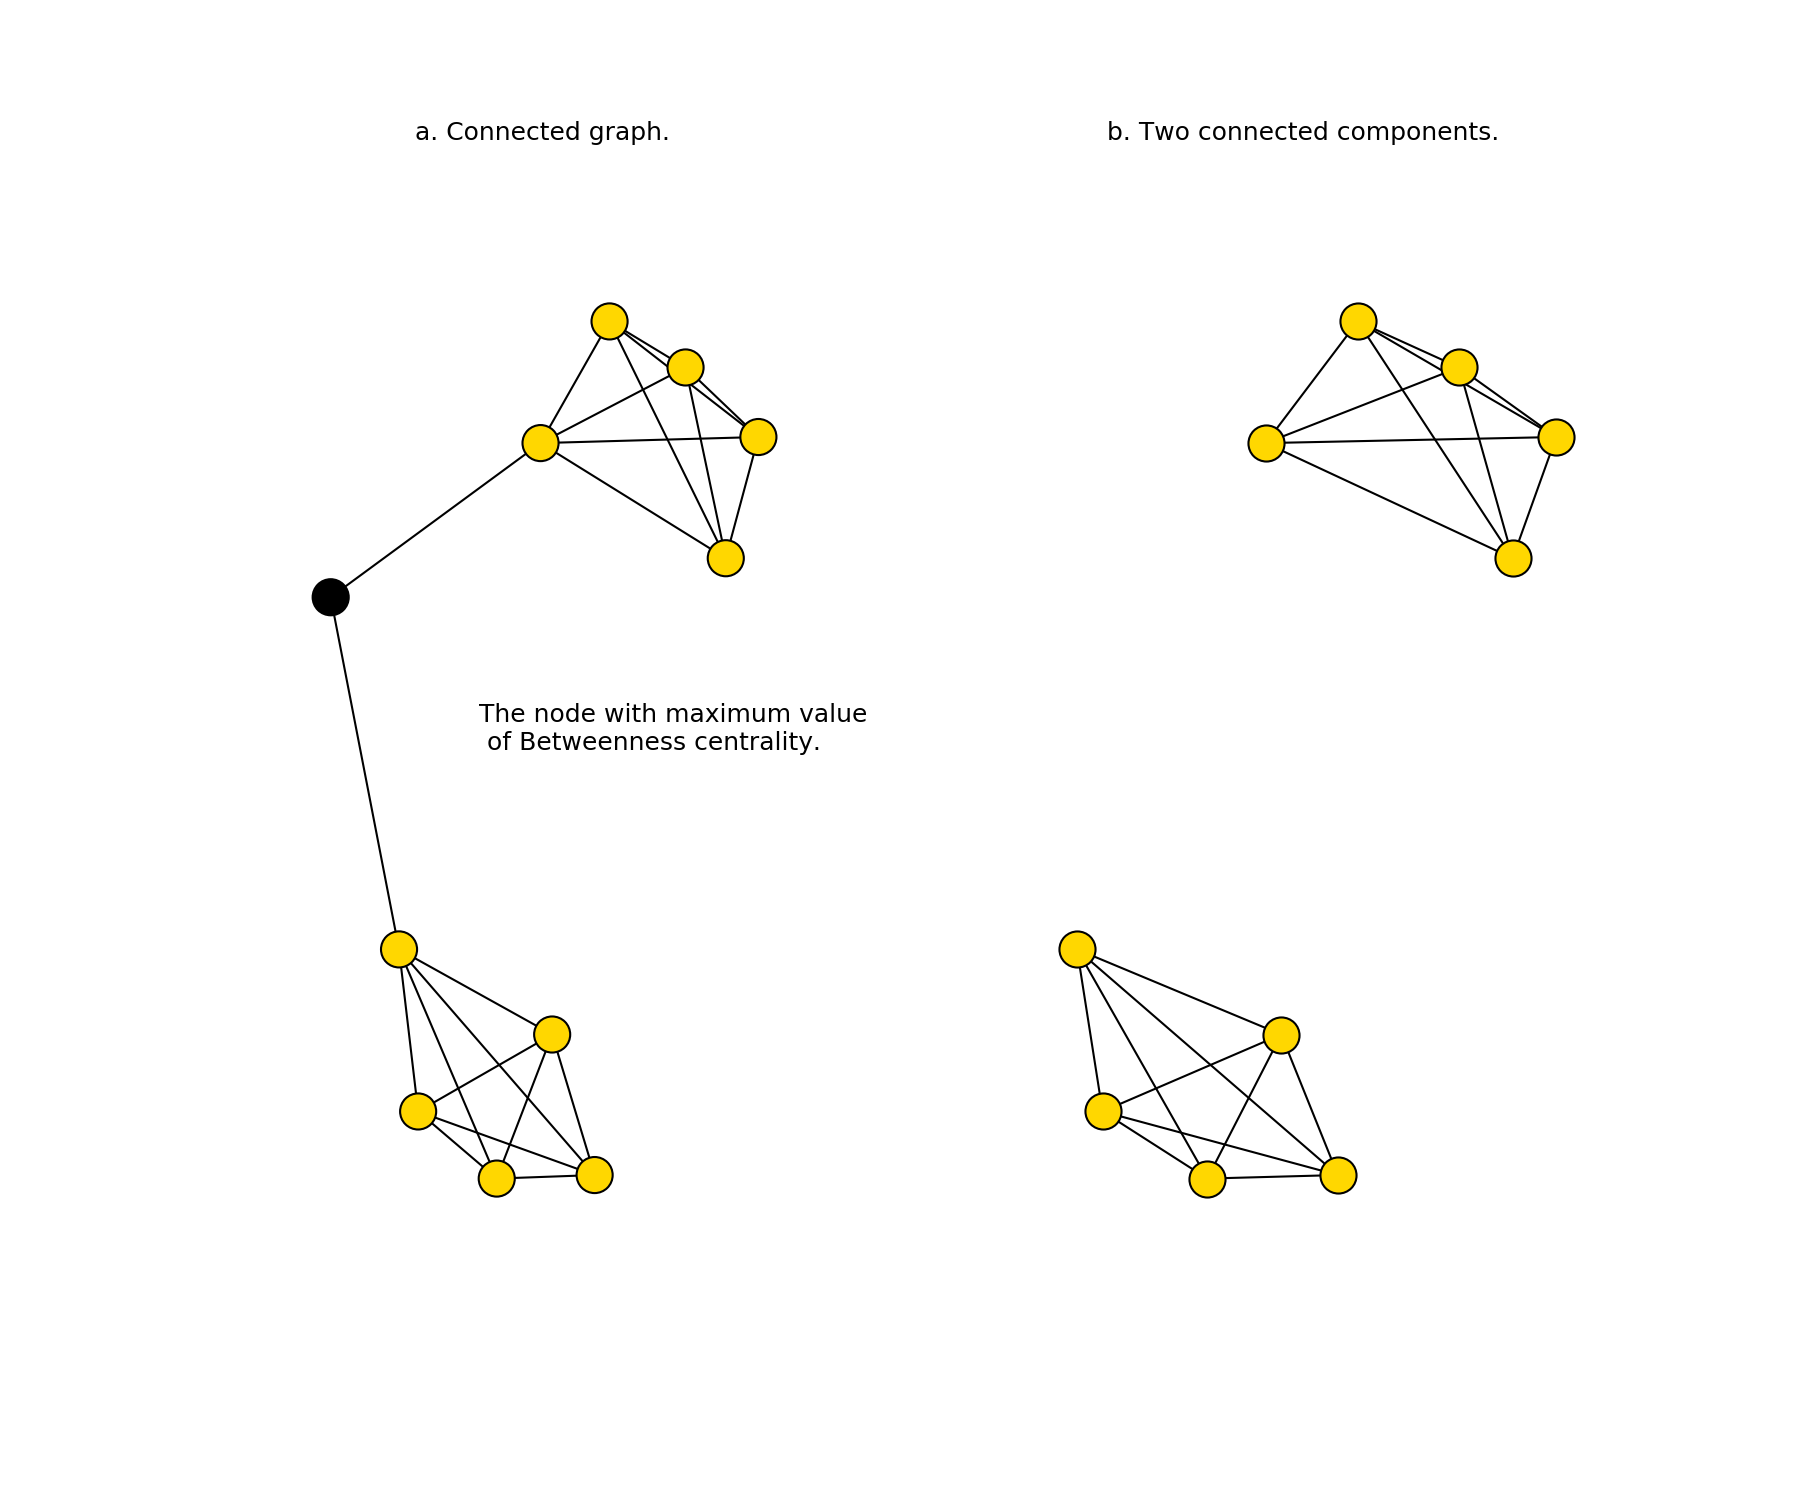
\includegraphics[width=\textwidth]{allo2eng.png}
	\caption{Graph separation model}
	\label{fig:allo2}
\end{figure}

Each of the components resulting from such separation can be analyzed for subjects homogeneity based on articles texts of which each component is formed. Several iterations would result in a set of clusters. 

The method proposed by the authors is a heuristic one and requires examination by a particular formal criterion. Conventional criteria for the purposes of clustering are proximity metrics for a cluster components and distances between components in separate clusters. 

Convergence of the authors’ method is ensured through searching a minimum of functional errors in determining $\mathit{k}$ clusters with  equation \ref{eq:allo1}.

\begin{equation} 
\frac{WSS}{BSS} -> min
\label{eq:allo1}
\end{equation}

Where $\mathit{WSS_{c_i}}$ –  within-cluster variation for cluster $C_i$, $m_i$ - centroid of $C_i$ and $i \in [1..k]$ (\ref{eq:allo2}).
The total $\mathit{WSS}$ measures the compactness of the clustering and we want it to be as small as possible.

\begin{equation} 
WSS = \displaystyle\sum_i^k\sum_{x \in C_i}\big(x - m_i\big)^2
\label{eq:allo2}
\end{equation}

And $\mathit{BSS}$ - weighted inter-cluster separation, measured by the between cluster sum of squares (\ref{eq:allo3}).

\begin{equation} 
BSS = \displaystyle\sum_j^k\sum_i^k \vert C_i \vert \big(m_j - m_i\big)^2
\label{eq:allo3}
\end{equation}

Where $ \vert C_i \vert $ - is a cluster size.

Interdisciplinary researches lead to the situation where articles may fall into several subject categories, thus the resulting clusters would be intersecting and non-exclusive.

The Gazpromneft STC publication activity has been chosen as a research subject. 
The data has been obtained from the OnePetro open on-line library of the international Society of Petroleum Engineers (SPE). 
Upon cleansing $172$ articles have been singled out.

Let us base our prediction on a co-authorship graph. 
For this purpose we build a co-authorship bipartite graph \cite{krasnov2018bi} with the nodes: author ($479$) and article ($171$). Authors have technical competences while articles have such attributes as title, year of publication and key words.

The resulting co-authorship graph has $26$ connected components of which the strongest one has $556$ nodes while the others have maximum eight nodes. 
Connected components with up to eight nodes represent the researchers’ first articles. 

Let us examine the strongest connected component (556 nodes). We extract a subgraph from the main co-authorship graph based on the nodes contained in the strongest connected component. The resulting subgraph is shown on the Figure \ref{fig:allo3} .

\begin{figure}[ht]
	\centering
	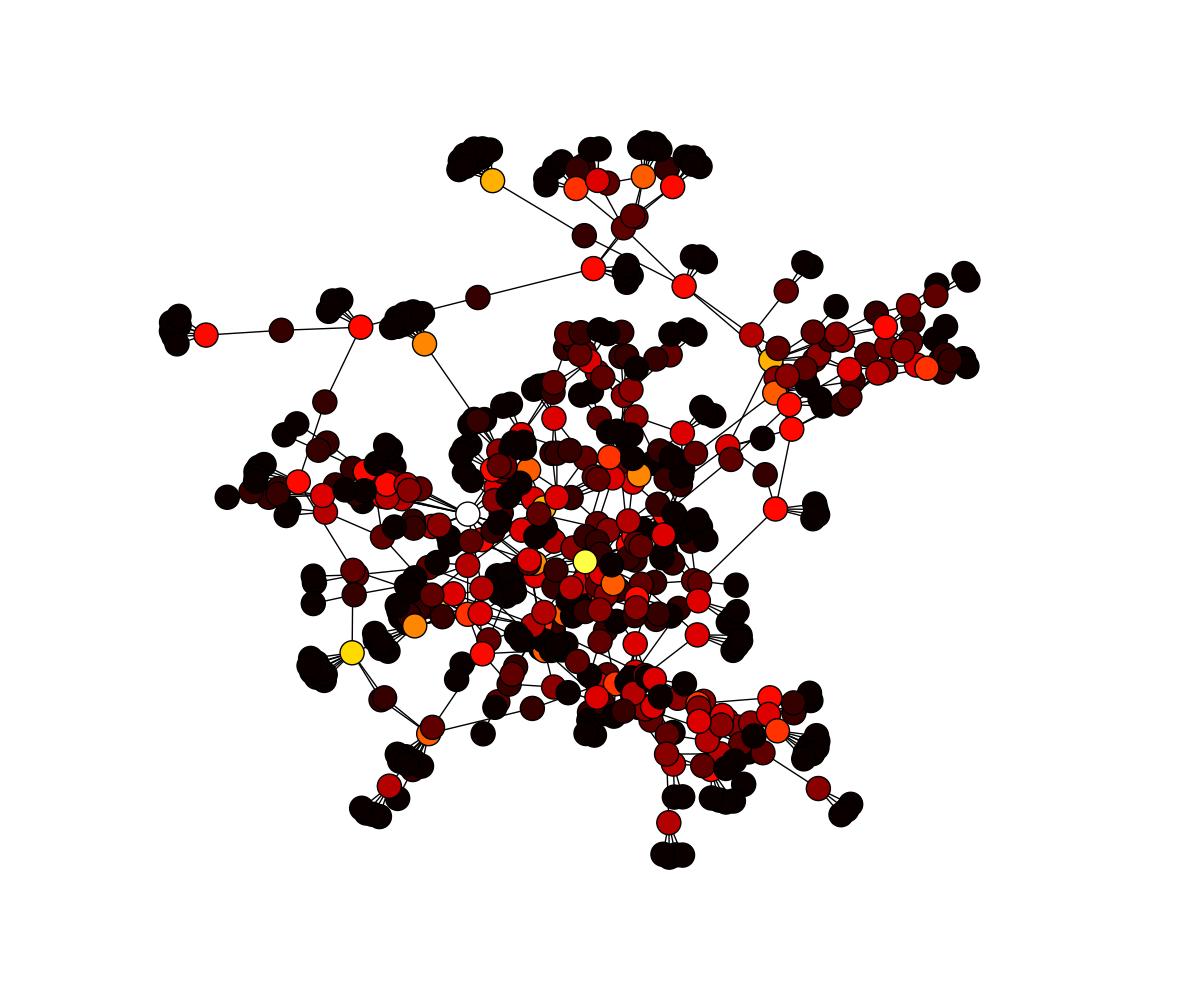
\includegraphics[width=0.6\textwidth]{allo3eng.png}
	\caption{Subgraph of the strongest connected component of the co-authorship graph of Gazpromneft STC.}
	\label{fig:allo3}
\end{figure}

Let us compute the Betweenness centrality metrics for the resulting subgraph. 
The obtained Betweenness centrality values are shown on the Figure \ref{fig:allo4}. 
Zero values for the Betweenness centrality are not shown.

%\begin{figure}[ht]
%	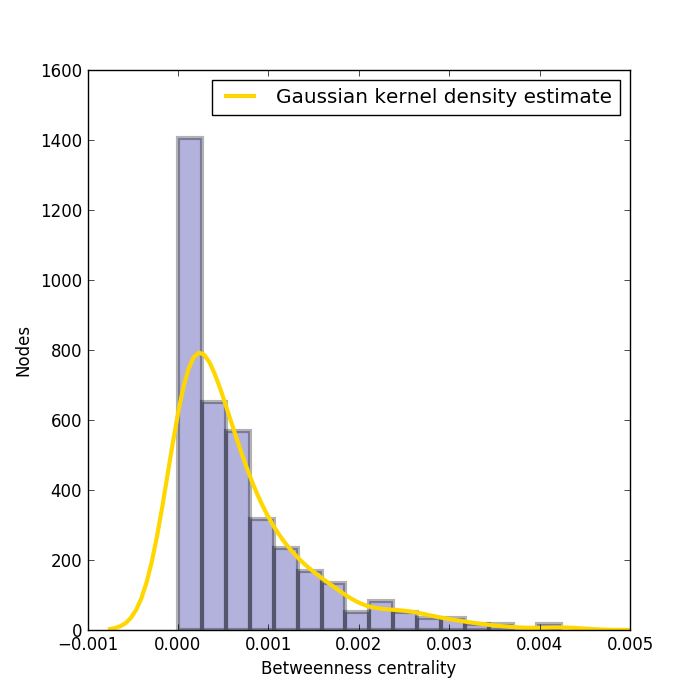
\includegraphics[width=\textwidth]{allo4eng.png}
%	\caption{Histogram of Betweenness centrality values for the subgraph of the strongest connected component of the co-authorship graph of Gazpromneft STC.}
%	\label{fig:allo4}
%\end{figure}

As we can see on the Figure \ref{fig:allo4} the values of the Betweenness centrality metrics in the third quartile belong to only $23$ nodes which represent less than 5\% of the total number of nodes. 

Let us apply the algorithm of artificial removal of the nodes with the highest value of the Betweenness centrality metrics. The Figure \ref{fig:allo5}  shows correlation between the connected components number and the number of artificially removed nodes.

%\begin{figure}[ht]
%	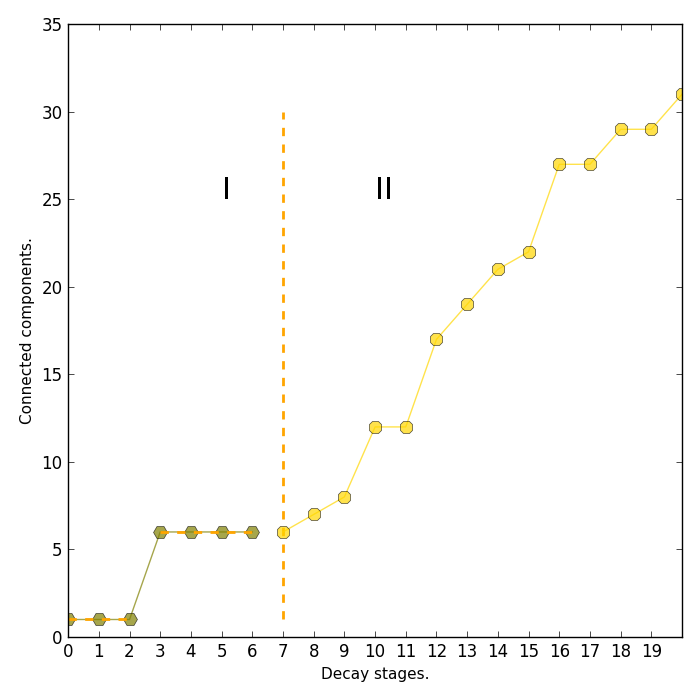
\includegraphics[width=\textwidth]{allo5eng.png}
%	\caption{Correlation between the connected components number and the number of artificially removed nodes.}
%	\label{fig:allo5}
%\end{figure}

As the nodes get removed the graph can behave in two following modes: 
\begin{enumerate}
	\item Connectivity constraint (Mode I)
	\item Exponential decay (Mode II)
\end{enumerate}

Mode I is characterized by the graph’s retaining its connectivity as the nodes with high values of the Betweenness centrality metrics get removed.  It means that the removed nodes are not the only connections between clusters.

Mode II is characterized by following the exponential model of a graph’s decay when each removed node causes exponential growth in emergence of new connected components.

Let us have a closer look at the second half of the Mode I of the algorithm when the graph has broken down into six connected components. These components’ sizes are $511, 34, 1, 1, 1, 1$. Among them the component with $34$ nodes shown on the Figure \ref{fig:allo6} represents the most pronounced direction of research into \textit{Subject 1}.

%\begin{figure}[ht]
%	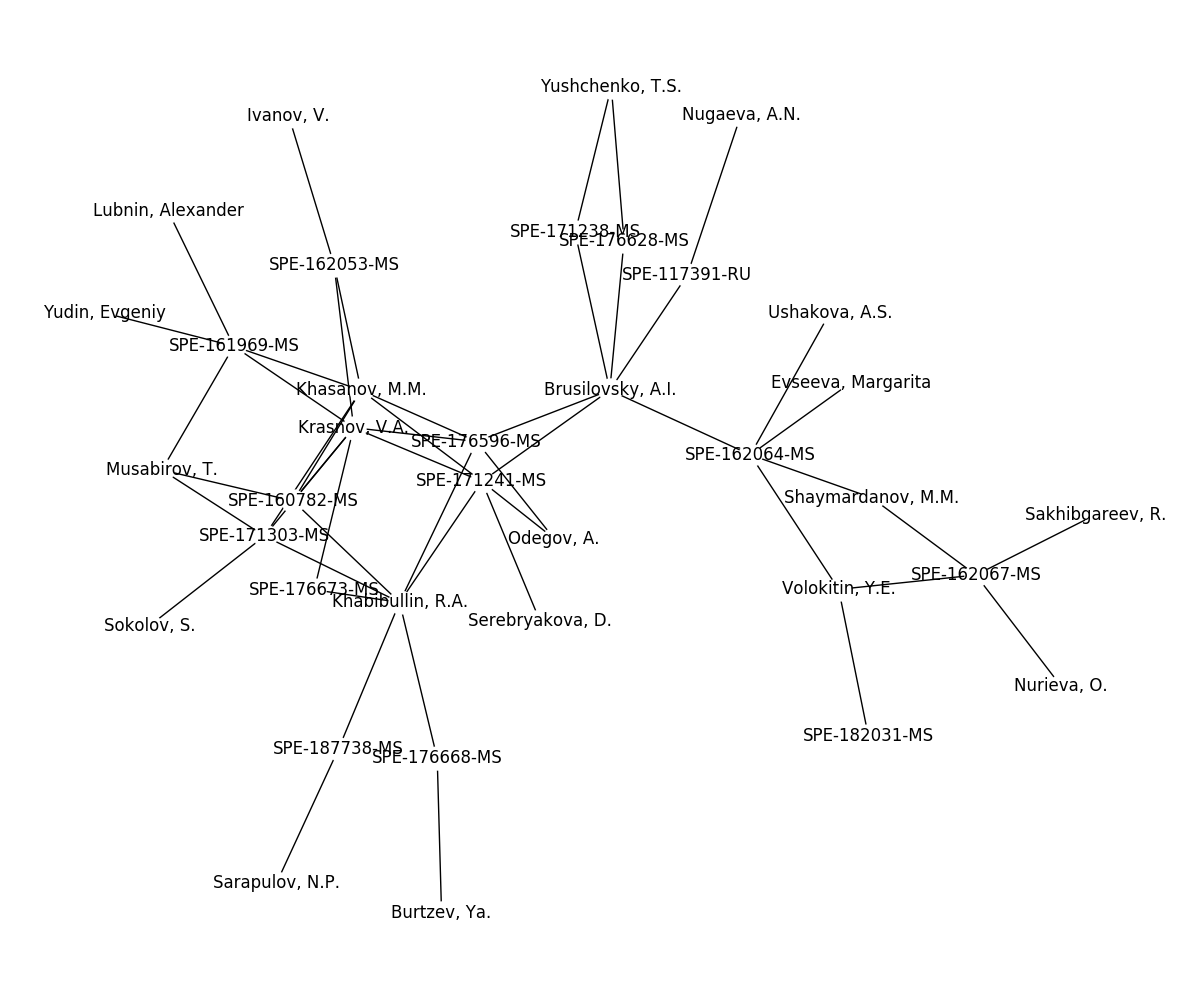
\includegraphics[width=\textwidth]{allo6eng.png}
%	\caption{The cluster of researchers into \textit{Subject 1} extracted through the method of removal of the nodes with the highest values of the Betweenness centrality metrics.}
%	\label{fig:allo6}
%\end{figure}

We have examined extraction of one cluster in detail. The complete algorithm of clusters extraction would consist of the following steps:
\begin{enumerate}
	\tightlist
	\item Building a co-authorship bipartite graph: $\mathit{G}$
	\item Finding the Betweenness centrality metrics for the $\mathit{G}$ graph
	\item Finding a node with $BC_{max}$ metrics (Betweenness centrality)
	\item Removing the $BC_{max}$ node (Betweenness centrality) from the $\mathit{G}$ graph
	\item Deriving a list of connected components of the $\mathit{G}$ graph
	\item Computing a quality metrics $WSS$ and $BSS$ of the retrieved clusters
	\item Further the algorithm is iterated for each connected component
	\item Algorithm is completed when all connected components represent clusters of acceptable quality.
\end{enumerate}

For the selected co-authorship graph $16$ clusters have been extracted. 
To compute values and W based on the articles texts we have applied the Vector Space Model (VSM). Each article is represented as a vector with the BM25 \cite{lv2011adaptive} metrics values for each word. Articles are considered as BOW (``bag of words''). For measuring distances between the articles’ VSM we have applied cosine measure. The Figure \ref{fig:allo7} shows the clusters separability matrix. Clusters’ numbers are on the axes. BSS function values are in the cells.

\begin{figure}[ht]
	\centering
	\includegraphics[width=0.7\textwidth]{allo7eng.png}
	\caption{Clusters separability matrix.}
	\label{fig:allo7}
\end{figure}

For the purposes of comparison of the resulting articles’ clustering we have performed clustering with the KMeans algorithm which yielded similar results (Figure \ref{fig:allo8} ).

\begin{figure}[ht]
	\centering
	\includegraphics[width=0.6\textwidth]{allo8eng.png}
	\caption{Comparison of the clustering algorithm proposed in this article with the KMeans algorithm.}
	\label{fig:allo8}
\end{figure}

The articles corpus has been broken down into clusters using the KMeans algorithm. 
The resulting clusters allowed arranging authors into groups.

\section{The probabilistic model of hidden topics based on the archive of the journal ``Oil Industry''.}

The question of which way applied science and technology is moving is key to any scientific and technological field. 
Traditionally, the definition of development vectors was made and is made by experts in the subject area, but a significant increase in the volume of information and an increase in the number of development directions indicate the need to Refine and improve this tool and develop additional methods of research of industry trends. 
In this study, the author analyzes the trends of the oil industry through automated text processing of scientific articles in the industry journal ``Oil industry''. 
Identifying the most common topics in the journal for the period from 2008 to 2016, we concluded that the importance of hard-to-recover reserves and the growing interest in the methods of development of such fields. 

The journal ``Oil industry'' is devoted to oil and gas problems.
It publishes articles on a wide range of issues in the oil and gas sector: economic, technical, technological, environmental and information. The publication dates back almost a century and has been published every month since 1920. 
All published articles are peer-reviewed.
The journal is included in The Russian science citation index (RSCI) and the international Scopus indexing system. 
Materials of the journal are in closed access and distributed by subscription. 
The main headings of the journal:

\begin{itemize}
	\tightlist
	\item oil and gas companies news;
	\item oil and gas industry;
	\item economics, management, law;
	\item geology and exploration;
	\item drilling;
	\item development and exploitation of oil fields;
	\item field design and construction;
	\item technology of oil production;
	\item oilfield equipment;
	\item transportation of oil;
	\item environmental and industrial safety;
	\item information technology. 
\end{itemize}

For the study, the editors kindly provided the archives of the articles of the journal ``Oil industry'' for the period 2008-2016. 
The sample contains 108 issues of journals, with articles from 3517 authors. 
Thus, a complete sample was obtained, which contained materials in a variety of substantive areas. 
On average, in the issue of ``Oil economy'' about 20-25 articles. 
The issues of the journal were considered, as they were the unit of analysis. 
The authors of the journal's articles are researchers, engineers and industry experts, many of them are candidates and doctors of science.

The research process had the following steps:

\begin{enumerate}
	\item
	Initially, the archives are presented as PDF files. 
	Sometimes it was a single file (binder) with articles for the whole year, and sometimes different files with individual articles. 
	In both cases, the files were intended for printing, that is, they contained a table of contents, page numbers, thematic inserts, and other editorial elements. 
	For the analysis, only texts in the form of sentences were needed, so the author implemented a software module to bring all the data to such a format. 
	It should be noted that, based on the chosen method, it was essential to keep the word order and division into sentences, while it was necessary to keep belonging to the issue, not to the article, as the minimum unit of interim analysis was chosen one issue.
	\item 
	At the second stage of the analysis, the words were reduced to the necessary forms. 
	For the analysis and comparison of words by methods of frequency and probabilistic analysis, it is necessary to narrow possible variants of the use of word forms. 
	There are several algorithms for solving text normalization task, in this case, stemming was used. 
	Stemming is the procedure of finding the basis of the word, and the basis and the root of the word may differ from each other.  
	One of the most common tools is Porter's stemmer, which, however, often trims the word more than necessary, making it difficult to get the correct word basis, such as ``stolovaia''->``stol''.
	Also, Porter's stemmer  cannot cope with all kinds of changes in the root of the word (for example, drop-down and fluent vowels), characteristic of the Russian language. 
	Therefore, the author focused on the use of the technology of stemming company ``Yandex'' - \textit{MyStem}. 
	This program produces a morphological analysis of the text in Russian. 
	It can build possible parses for words that are not included in the dictionary and offers several options for the basics of the word. 
	However, the author found it necessary to maintain a reverse dictionary for the resulting word forms in order to maintain the relationship between the original word and the resulting word form. 
	Abbreviations widely used in the oil and gas industry were treated as a separate branch. 
	Definition of abbreviations was based on the dictionary of abbreviations established and supported in the company GazpromNeft in the framework of the project of Corporate Wikipedia \cite{khasanov2016corporate}.
	\item 
	At the third stage of the study, the formation of the dictionary was carried out. 
	It is known that the most significant semantic weight are not single words, but combinations of words, in particular pairs of words – bigrams. 
	The author used heuristic algorithms to distinguish bigrams. 
	A matrix of bigrams in the neighborhood of five words for each of the sentences was compiled. 
	Then we calculated the frequency of use of each of the bigrams, after which were recorded 5\% of the most common phrases.
	\item
	In the fourth stage, the vocabularies of individual words and bigrams were combined for the overall treatment algorithms of allocation of subjects. 
	The resulting dictionary was analyzed for the selection of high and low-frequency words for their filtering. 
	Traditionally, the final generation of the dictionary is made with the help of stop words. 
	The author did not use algorithms of stop words selection in this article. 
	This decision was because the addition of a dictionary of stop words did not add accuracy to the study.
	\item 
	At the final fifth stage, a model of topics was built. 
	The BigARTM \cite{ianina2017multi} tool was used to build the topic model. 
	At this stage, we obtained the matrix distribution of topics for the document ($\Theta$) and the distribution of words for the topic ($\Phi$). 
	To improve the accuracy of the algorithm, the author applied an analytical approach that clarifies the regularization parameters.
\end{enumerate}

The primary metric for detecting convergence of the topic model is the Perplexity metric. 
The curve of the dependence of Perplexity on the number of iterations on the body of texts is shown in figure \ref{fig:nx1}.

\begin{figure}[ht]
	\centering
	\includegraphics[width=0.6\textwidth]{nx1}
	\caption{The Perplexity score for the body of texts.}
	\label{fig:nx1}
\end{figure}  

From the figure \ref{fig:nx1}, it can be seen that in three passes the topic model showed acceptable convergence and did not need further optimization. 

Essential quality metrics of the model are the degree of the sparseness of the matrices $\Phi$ and $\Theta$. 
These metrics can be controlled by the parameters $\tau$ corresponding to the regularizers. 
In the figures \ref{fig:nx2} and \ref{fig:nx3} dependencies for the sparsity of $\Phi$ and $\Theta$ matrices are displayed.

\begin{figure}
	\centering
	\begin{minipage}{.5\textwidth}
		\centering
		\includegraphics[width=0.9\linewidth]{nx2}
		\caption{The degree of the sparseness of $\Theta$ from $\tau$ dependence.}
		\label{fig:nx2}
	\end{minipage}%
	\begin{minipage}{.5\textwidth}
		\centering
		\includegraphics[width=0.9\linewidth]{nx3}
			\caption{The degree of the sparseness of $\Phi$ from $\tau$ dependence.}
		\label{fig:nx3}
	\end{minipage}  
%	\caption{The degree of the sparseness of the matrices $\Phi$ and $\Theta$.}
%	\label{fig:nx2-3}
\end{figure}

Based on the dependencies shown in figures  \ref{fig:nx2} and \ref{fig:nx3} the author chose the regularization parameters of the topic model, which allow achieving an optimal ratio between essential terms and noise.

The thematic model obtained as a result of this study can be presented in various forms. The level of noise terms makes it difficult to interpret the results, so there are six substantive topics from the planned twelve. 
The table \ref{tab:nx1} presents the topics calculated by the model.

\begin{table}[H]
	\centering
	\caption{Fragment of the matrix $\Phi$ for terms with maximum probabilities.}
	\label{tab:nx1}
	\resizebox{\textwidth}{!}{%
		\begin{tabular} {|l|l|l|l|l|l| }
			\hline
			\textbf{Topic1} & \textbf{Topic2} & \textbf{Topic3} & \textbf{Topic4} & \textbf{Topic5} & \textbf{Topic6} \\ \hline
			электронный & ЭЦН & сдвиг & почва & нефтегазоносность & ингибитор \\ \hline
			знание & УЭЦН & сигнал & добавка & свод & разлом \\ \hline
			автоматизация & сероводород & окисление & композиция & компания & деформация \\ \hline
			интегрировать & фациальный & разрушение & знание & впадина & трещиноватость \\ \hline
			пользователь & гамма & деформация & агрегат & сепарация & исследовательский \\ \hline
			архив & доломит & реологический & загрязнение & миграция & известняк \\ \hline
			хранение & замер & песчаный & ПЗП & прогнозный & порода \\ \hline
			доступ & депрессия & осадки & надежность & активность & политехнический \\ \hline
			подразделение & агент & капиллярный & камень & филиал & штанга \\ \hline
			платформа & каротаж & сечение & окисление & цемент & приемистость \\ \hline
		\end{tabular}%
	}
\end{table}

It is safe to say that the terms collected in the column \textit{Topic 1} characterize the subject of knowledge management. 
In column \textit{Topic 2} are the subject of extraction. 
The other columns can also be quite unambiguously interpreted. 
Moreover, for machine processing, a set of terms is more important than its generalizing theme.

\begin{figure}[H]
	\centering
	\includegraphics[width=0.94\textwidth]{nx4}
	\caption{Matrix $\Theta$.}
	\label{fig:nx4}
\end{figure} 

In the figure \ref{fig:nx4} the $\Theta$ matrix is presented, giving an idea of how the topics obtained are distributed in each of the analyzed releases. 
We can see that the theme with \textit{Topic 9}  is presented in all editions  – it has shared information, greetings, and advertising. 
The resulting view also allows we to select the most relevant releases with a specific topic. 

It is important to note that the method chosen by the author has shown a high speed of analysis, which makes it possible for use in online search processes. 
For example, on the website of the publishing house as a means of improving the search and giving recommendations to readers on articles with similar topics. 
It should also be noted that this technique can be further improved and adapted for the analysis of significantly large amounts of dynamic data and highlight critical areas of technological development in both broader and narrower areas.

\section{Topic Classification Through Topic Modeling with Additive Regularization for Collection of Scientific Papers}

Topic Modeling is one of the current directions in statistical procession of natural languages. 
The Probabilistic Latent Semantic Analysis (PLSA) \cite{hofmann2017probabilistic} of a collection of documents describes each topic through discrete probability distribution of words, while each document as a discrete distribution of topics.

Through this approach one can build an infinite number of various mathematical models for collections of documents. In practice for the purpose of Text Mining one needs ``good''  topic models: topics should be homogeneous and have unique content.

There are several dozens of various methods of building topic models. The most popular one is the method of building a topic model based on the Latent Dirichlet Allocation (LDA) suggested by D. Blei  in 2003 according to the following formula:

\begin{equation} 
\label{eq:op1}
p \left( d \vert w \right) = \sum_{t \in T} p \left( w \vert p \right) \; p \left( t \vert d \right)
\end{equation},
where $T$ is a set of topics, $p(t)$ is an unknown distribution of topics over the entire collection, $p(d)$ is a prior documents distribution (estimation $\frac{n_d}{n}$),  $p(w)$ is a prior distribution in a word set ($\frac{n_w}{n}$). 

Based on the equation (\ref{eq:op1}) we can introduce the following entities:  

\begin{itemize}
	\item $ \theta_d = \big( p \left( t \vert d \right) : t \in T \big) $ -- probability vectors of documents,  $\vert T \vert  \sim  Dir \left( \theta , \alpha \right) , \quad \alpha \in \mathbb{R}^{dim \vert T \vert}$, 
	\item $ \phi_t   = \big( p \left( w \vert t \right) : w \in W \big) $ -- probability vectors of topics, $ \vert W \vert \sim Dir \left( \phi, \beta \right) , \quad \beta \in \mathbb{R}^{dim \vert W \vert}$.
\end{itemize}

Practical experience shows that topical modeling based on the LDA model not always brings as well interpretable results as the ones mentioned in the original article \cite{blei2012probabilistic}: topics contain ``empty'' words, it may be difficult to attribute the obtained topic to a particular class, the words contained in the topic most probably do not describe the topic. 

Many practical researchers have noted that the LDA topic model does not overfitting itself as the PLSA does; however, from the Author's experience, this is not the case for the large collections of documents. 
It should be noted that the very concept of overfitting is not quite applicable to mathematical models, as the problem of generalization of a new text based on the topic model is not set in practice. As a rule practical researchers use ready sets of documents and solve a problem of getting information of this particular collection's hidden structure.

Topics extracted from collections of documents often contain noisy words and cannot be sufficiently interpreted, even by experts. The very need for experts for determine topics names makes automatic processing of documents collection very cumbersome.  

Another issue in the topic modeling is that the obtained topics do not have any priorities or any other features which would make their interpretation easier. Such as a topic's degree of authenticity or its weight in a document. 
For this reason the obtained topics need additional heuristic modifications in order to make them ``brushed up''. Which suggests that such ``brushing up'' could be done even during the model training process.  In other words, there are certain rules for obtaining $\theta_d$ and $\phi_t$ during the training process which may affect the quality of the obtained topics. 

%Given this, the Author has formulated the following research hypothesis:
%
%\fbox{%
%	\parbox{0.95\textwidth}{%
%		Hypothesis 1.\\
%		If a collection of documents can be presented as triads\\
%		$\Omega_n = \left( w_i , d_i, t_i \right), \; i \in \left( 1, \dots , n \right) $,\\
%		where $w_i$ are words, $d_i$ are documents, and $t_i$ are hidden topics,
%		for each hidden topic $t_i$ there would be a single class
%		$C_j, \; j=1, \dots, m $  and  $m \ll n$.
%		And $C$ are the classes of the hidden topics.
%	}
%}


The essential rationale of the method described in this paper is setting aside the Dirichlet prior allocation and considering potential improving of the PLSA topic model in order to obtain more interpretable topics.

A series of researches like \cite{vorontsov2015additive, vorontsov2014additive, vorontsov2015additive2} support the presumption that the PLSA probabilistic topic model can be improved through additive regularization. Additive regularization of topic models (ARTM) is a multicriteria approach where a probabilistic topic model is optimized based on a weighted sum of criteria.

The paper \cite{voron2013mod} presents the method of developing an ARTM topic model which allows managing the training process through adding to the authenticity function, at the training stage, such regulators such as:

\begin{equation} 
\label{eq:op2}
R\left( \Phi ,  \Theta \right) = \sum_{t \in T } \sum_{w \in W}  \beta_{wt} \ln \left( \phi_{wt}\right) + \sum_{d \in D} \sum_{t \in T} \alpha_{td} \ln \left( \theta_{td} \right)
\end{equation},
where $\beta_{wt}$ and $\alpha_{td}$ are regularization coefficients.

This approach to the management of the quality of probabilistic topic model has been proposed by Prof. K.V. Vorontsov. 

The probabilistic topic model of text generation describes the process of documents collection formation through known distributions $p \left(w \vert t \right)$ and $p \left( t \vert d \right)$. 
The topic modeling problem is the reverse one: for a given collection $D$ to find matrices of coefficients $\phi_{wt} $ and $\theta{td} $ with which the following condition is true:

\begin{equation} \label{eq:op3}
p \left( w \vert d \right)  \approx \sum_{t \in T} \phi_{wt}  \theta_{td}
\end{equation}

The model training under the ARTM method is based on the reduced EM--algorithm which is used for iterated search of non-linear equations for $\phi_{wt}$ and $\theta_{td}$. 

Each topic's semantics is described as a $\phi_{wt}$ matrix. 
Therefore, to manage the quality of a topic model through regulators $\tau_i R_i \left(\Phi , \Theta \right)$ one can use various approaches in their sequenced combination so that each them would prepare the model for processing in the subsequent training iterations. 
Each approach can be described as a function setting values for $\tau_i$ coefficients depending on iteration step.  
However, how many iterations would be required for each approach, depends on such factors as the collections' vocabulary capacity and the sufficiency of documents.

Through the diversity of approaches $R_i \left( \Phi , \Theta \right)$ each topic's semantics $\phi_{wt}$  changes. On Figure \ref{fig:op4} is shown how the ``document-topic'' space transforming  in process of regularization.

\begin{figure}
	\centering
	\includegraphics[width=0.85\textwidth]{op3fig4eng.png}
	\caption{The ``Document-topic'' space transformation.}
	\label{fig:op4}
\end{figure}


The theory shows that it is possible to form the ``black'' and the ``white'' lists of topics through making matrices $\phi_{wt}$ and $\theta_{td}$ \cite{vorontsov2015bigartm} smooth or sparse, determine ``main'' and ``auxiliary'' topics \cite{vorontsov2015non} as well as decorrelate topics by excluding repeated and linearly dependent topics \cite{vorontsov2014tutorial}. 
However, experiments with particular collections of documents are still to support these theoretic assumptions.

It is important to note that in the process of training a convergence matrix will be the Perplexity calculated as follows:

\begin{equation} 
\label{eq:op4}
P \left(D,\Phi, \Theta \right) = exp \bigg( \frac{-1}{n_d} \sum_{d \in D} \sum_{w \in d} n_{dw} \times \ln \bigg( \sum_{t \in T} \phi_{wt} \theta_{td} \bigg) \bigg)
\end{equation}

The \textit{Perplexity} matrix is not normed and, therefore cannot be used in comparing various models convergence. The general essence is, that the smaller \textit{Perplexity}, the better a model. 
That is why in making decisions on sufficiency of convergence the criterion is whether \textit{Perplexity} stops significantly decreasing as the number of training iterations grows.

The Author has used a collection of documents from the work \cite{krasnov2018bi}, containing 1696 science and technology articles in English from the OnePetro e--library. 
All the articles in the collection are dedicated to oil and gas industry.

In the beginning, the Author has trained the PLSA topic model in order to establish the speed of convergence in respect to the \textit{Perplexity} matrix. \textit{Perplexity's} dependence on the number of the model training epochs is shown on Figure \ref{fig:op1}.

\begin{figure}
	\centering
	\includegraphics[width=0.65\textwidth]{op3fig1eng.png}
	\caption{Correlation of \textit{Perplexity} to number of epochs.}
	\label{fig:op1}
\end{figure}

The dynamics of the \textit{Perplexity} convergence shows that this model version gets converged pretty fast. From the 10th iteration any further changes of the \textit{Perplexity} metrics become insignificant.

In this experiment the Author's task was to divide topic into the basic and the auxiliary ones. 
From the perspective of regularization it means that the noisy topics would be smoothed while the basic ones get sparse in the process of the model's training. 
From the Equation (\ref{eq:op2}) it follows that for smoothing coefficients $\beta_{wt} $ and $\alpha_{td}$ have to be negative, and for sparsity -- positive. 

The obtained result can be presented in a graphical mode as a map of the matrix $\Theta$ coefficients. 
Let us consider the result of the model's distributing documents into particular topics. 
Distribution of topics for each document is shown in the $\Theta$ matrix.  
To obtain a more general idea of the $\theta$ matrix' transformation the author have represented it as charts before (Fig. \ref{fig:op2}) and after (Fig. \ref{fig:op3}) regularization.

\begin{figure}
	\centering
	\begin{minipage}{.5\textwidth}
		\centering
		\includegraphics[width=0.95\linewidth]{op3fig2eng.png}
		\caption{The $\Theta$ matrix before regularization. Numbers of documents in the collection are marked on the x -- axis.}
		\label{fig:op2}
	\end{minipage}%
	\begin{minipage}{.5\textwidth}
		\centering
		\includegraphics[width=0.95\linewidth]{op3fig3eng.png}
		\caption{The $\Theta$ matrix after regularization. Numbers of documents in the collection are marked on the x -- axis.}
		\label{fig:op3}
	\end{minipage}
\end{figure}

As we can see in the figure \ref{fig:op2}  and figure \ref{fig:op3} the $\Theta$ matrix in the process of regularization becomes sparser in the basic topics (\textit{sbj0} -- \textit{sbj10}) and more compressed in the auxiliary topics (\textit{nz0} -- \textit{nz1}). 

The vocabulary of the auxiliary topic is quite significant. The Table \ref{tab:op1} below shows auxiliary topics before and after regularization.

\begin{table*}[tbp]
	\centering
	\caption{Top10 terms forming auxiliary topics before and after regularization learning.}
	\label{tab:op1}
	\begin{tabular}{|l|l|l|l|}
		\hline
		\multicolumn{2}{|l|}{\textbf{Before regularization}} & \multicolumn{2}{l|}{\textbf{After regularization}} \\ \hline
		\textit{nz0} & \textit{nz1} & \textit{nz0} & \textit{nz1} \\ \hline
		pump & wave & pump & stress \\ \hline
		pipeline & seismic & sand & equation \\ \hline
		esp & seg & completion & seismic \\ \hline
		power & frequency & injection & wave \\ \hline
		subsea & velocity & tubing & velocity \\ \hline
		operating & waves & equipment & numerical \\ \hline
		lift & amplitude & operating & elastic \\ \hline
		equipment & x & downhole & array \\ \hline
		installation & elastic & power & impedance \\ \hline
		liquid & offshore & esp & direction \\ \hline
	\end{tabular}
\end{table*}

Noteworthy is that the seismic (\textit{nz1}) topic is among the auxiliary ones. 
According to an expert, such words as seismic, wave, velocity, elastic, seg, frequency and amplitude relate to seismic.
Articles on seismic are rare on the OnePetro platform and indeed can be considered secondary. 
After regularization learning several terms related to calculation appeared in the \textit{nz1} but the seismic topic remained.
In particular, the offshore term has gone to the basic topics. 
Situation with the \textit{nz0} topic is quite clear. 
It includes the most frequently used words which are not actually noise.

Let us also pay attention to the quantitative analysis of the $\Theta$ matrix coefficients. 
For example the document No. 555 has the biggest topic weight 0.72 (\textit{sbj6}).
Probabilities of other primary topics for this document are close to zero. 
Thus, this document according to the model is fully focused on the sbj6 topic represented by words: recovery, injection, steam, core, viscosity, flooding, solvent, heavy, saturation, surfactant. 
With the help of an expert the \textit{sbj6} was named ``Chemical Enhanced Oil Recovery''.

On the other hand, we can find in our sample of texts corpus that this document correlates to the article with the title ``Low Tension Gas Process in High Salinity and Low Permeability Reservoirs''. 
Here is an abstract from the public summary of this article on the OnePetro.org \footnote{https://www.onepetro.org/conference-paper/SPE-179839-MS} :

\fbox{%
	\parbox{0.90\textwidth}{%
		\texttt{Abstract}\\
		\texttt{Chemical enhanced oil recovery (EOR) in carbonate reservoirs has always been technically and economically challenging. Conventional Alkaline-Surfactant-Polymer (ASP) flooding has limited application in low permeability (2-20 mD) and high salinity formations (~200,000 ppm TDS) with a large concentration of divalent cations. Also injectivity into such low permeability reservoirs can be a significant problem with polymer solutions} $\dots$. \\
	}
}

As we can see from the public abstract from the article, its subject is highly specific. 
Moreover, based on the model we know that this article is indeed focused on this subject. 
When subscribing for this article one can be confident that it would not have other topics. 

It is also worth noting that an expert's help was not essential for retrieving the \textit{sbj6} topic's title; instead one could avail oneself of the fact that the document was represented by one single topic and find its title in the article's summary. 

\section{Analysis of Strong and Weak Ties in Oil\&Gas Professional Community}
The importance of weak social ties in professional communities is well studied and widely accepted.
In our paper we analyze the structure of strong ties based on the co-authorship relation and use the formal concept analysis framework to figure out weak ties.
The research is motivated by fast growing need in cross-disciplinary research, which requires experts from different areas to understand the bigger picture and identify potential fellows for collaborative research projects in nearest future.

The goal is to develop a methodology and tools for automated analysis of a collection of research papers available at the SPE digital library.
On the basis of these analyzes one should be able to:
\begin{itemize}
	\item figure out the most important and relevant research topics,
	\item assess the influence of different researchers and scientific schools,
	\item identify strong and weak ties in the professional community, \end{itemize}
and use all of these in daily research management process.
This paper is focused on the third item in the list. It continues our study of professional communities started in 
\cite{KrYav_BI,krasnov2013comparison,krasnov2014connectivity,krasnov2014indicators,barysheva2015profiling,barysheva2015building,sofia2017structure}

The analysis of social networks  of co-authorship has a long history \cite{hou2008structure}. There are a plenty of studies examining the structure of co-authorship ties within diverse scientific fields and reveal specific collaboration patterns for the different disciplines \cite{acedo2006co,barabasi2002evolution,ding2011scientific,newman2001structure,rodriguez2008relationship}.
Here we intend to uncover weak social ties in the Oil\&Gas professional community. This is similar to the task of link prediction in social networks, see e.g. \cite{wang2015link}.

Weak ties within social networks is one of the key concepts. The idea of the differentiation of ties by their strength was firstly considered by sociologist Granovetter in \cite{granovetter1973strength}, who empirically showed that weak ties (e.g. ties with not very close friends and relatives) are of a great importance in case of information propagation and knowledge diffusion. In case of Granovetter, weak ties were the source of the important information about working places and vacancies.

The identification of weak ties within a professional community has a great practical importance. Firstly, identification of people who are working on the same topic and substantial research idea is very important for information gathering and knowledge diffusion. Secondly, knowing the social environment, e.g. 'weak ties' within the community can be important in collaboration and cooperation establishment. 

This study is based on materials of annual SPE Russian Oil and Gas Conference and Exhibition 2016. 
The main features of this event are as follows:

\begin{itemize}
	\item  Multi-disciplinary. The conference presentations, selected on the basic directions of development Oil \& Gas industry. These areas are listed below.
	\item  Periodic. This is an annual conference.
	\item  Regional. The majority of the participants represented mainly the Russian companies.
	\item  High selection criteria. The conference acceptance rate is approximately 15\%. The selection process is conducted by Subject Matter Experts.
	\item The conference program consists of four parallel sections.
	\item At least one co-author must attend the event and present the work.
\end{itemize}

The data we work on is retrieved from open portal of Society of  Petroleum Engineers (SPE) at  \url{http://www.onepetro.org}. 

Clean up and preparation of meta information was produced using Python on hybrid cluster at Gazpromneft STC. Text analysis was done using Python NLTK library. Statistical analysis was performed using SciPy library.

The collection comprises 404 articles written by 839 co-authors. It includes papers in the following areas:
\begin{enumerate}
	\item Well construction – drilling and completion.
	\item Static and dynamic modeling.
	\item Hard-to-recover reserves.
	\item Well and formation testing.
	\item Field development monitoring and control.
	\item Well intervention.
	\item Shelf development experience and prospects.
	\item Field geophysical survey/well logging.
	\item Gas condensate and oil gas condensate field development.
	\item Brownfields.
	\item Geomechanics.
	\item Oil and gas production - equipment and technologies.
	\item Cores recovery, examination and analysis
\end{enumerate}

In the retrieved data each publication record includes the following information:
\begin{itemize}
	\item title and abstract of the article;
	\item the list of authors and their affiliations; 
	\item year of publication.  
\end{itemize}

The most time-consuming step was to prepare the data and make the data set clean and useful. 
Unfortunately, the portal does not have a directory for authors. 
As a result sometimes we had up to 6 different spellings of the same name in different articles.

Almost every paper in the collection is written jointly by a few authors. It usually takes at least several months to write a good paper, so in the context of professional community each publication could be considered as a proof of strong ties between the co-authors.

%\begin{figure}[ht]
%	\centering	
%	\includegraphics[width=0.85\textwidth]{wt1eng}
%	\caption{{\bf Visualization of the strong ties in  Oil\&Gas professional community.} }
%	\label{fig:wt1}
%\end{figure}

In figure \ref{fig:wt1} nodes are authors, links correspond to the co-authorship relation. The graph has 839 nodes, 2315 ties, 127 components.
The descriptive statistics for the co-authorship network is given below.

\begin{itemize}
	\item Number of nodes: $839$
	\item Number of strong ties: $2315$
	\item Number of connected components: $127$
	\item Size of the largest connected component: $198$
	\item Size of the second largest connected component: $20$
\end{itemize}

This and the other graphs in this paper are produced with yEd Graph Editor \cite{wiese2004yfiles}.

An inspection of the largest connected component shows that it mostly consists of participants of the well established collaborative program between Gazprom subsidiaries and Schlumberger. Otherwise the picture is very typical for a large industrial research conference, where the audience consists of big number of small cliques, which hardly communicate with each other.

As it was already mentioned above the goal of our work is to help the members of a professional community identify participants with similar interests and then convert weak ties into strong ones by establishing mutually beneficial collaborative research projects.

The importance of weak ties is well studied in the literature, see \cite{granovetter1973strength,granovetter1983strength}.
In this paper we assume that two researches have weak ties if they both work with the same objects or concepts. We believe that if two persons work on the same substantial problem (e.g. they share same narrow research topic), they should at least know each others' works. We assume these social ties are weak, because they are very much likely to know each other and even communicate, but the intensity of their interactions and communications is very much likely to be low, because they are not involved in joint projects.

The heuristics is implemented in the following way. 
First, we start from extracting keywords for each paper in order to create a formal context, i.a. object-attribute relation in which objects are words, attributes are authors, and the relation is {\it ``a keyword $w$ is used by an author $a$''}. 
Second, the association rules with high characteristics of support and confidentiality are computed using Concept Explorer tool, see \cite{yevtushenko2006conexp,yevtushenko2000system}.

Finally, for every association rule of the form:
\begin{equation}
a_1, \ldots, a_m \Rightarrow b_1, \ldots, b_k, 
\end{equation}
where $a_1, \ldots, a_m, b_1, \ldots, b_k$ are author IDs we assume that all members of the joint group $\{a_1, \ldots, a_m,b_1, \ldots, b_k\}$
are weakly connected.

As it was mentioned above our data set stores titles and abstracts of papers. As these texts are rather small we initially consider all words as equally important.

After the clean up the object-property table has 729 objects (keywords) and 839 attributes (authors).


On table \ref{tab:wt1} several examples of the association rules are presented. Each rule has two parts, antecedent and consequent, which are set of attributes. Support indicates the number of objects, which share these attributes. In our case, support is the number of keywords common for all authors in the set.

\begin{table}[H]
	\caption{Examples of the computed association rules. Attributes are authors' IDs, support is the number of common keywords for these authors.}
	\label{tab:wt1}
	\begin{center}
		\renewcommand{\arraystretch}{1.5}
		\label{my-label}
		\begin{tabular}{|c|c|c|c|c|}
			\hline
			Support & Antecedent attributes & Confidence & Support & Consequent attributes \\\hline\hline
			17 & 564;825 & $=$ 94\% $\Rightarrow$ & 16 & 133 \\
			16 & 335;636 & $=$ 94\% $\Rightarrow$ & 15 & 226;131;542;552    \\
			15 & 131;335 & $=$ 100\% $\Rightarrow$ & 15 & 226;542;552;636   \\
			16 & 101;436 & $=$ 88\% $\Rightarrow$ & 14 & 132   \\
			15 & 801;357;510 & $=$ 93\% $\Rightarrow$ & 14 & 8   \\
			15 & 333;754 & $=$ 93\% $\Rightarrow$ & 14 & 42;133\\  
			6 & 108;233 & $=$ 83\% $\Rightarrow$ & 5 & 754\\  
			\hline
		\end{tabular}
	\end{center}
\end{table}

In figure \ref{fig:wt2} nodes are authors, co-authorship relation is represented by blue solid links, the dashed red edges correspond to the weak ties. Grey boxes set out previously disconnected fragments, which get bridged with the weak ties.

%\begin{figure}[ht]
%	\centering
%	\includegraphics[width=0.85\textwidth]{wt2eng}
%	\caption{Visualization of the largest connected component with the weak ties.}
%	\label{fig:wt2} 
%\end{figure}

The main idea here is to interpret each association rule as an evidence of common interests for the involved authors. For example, from rule
$$
15 \; | \; 333;754 \; = 93\% \Rightarrow \;  14\; | \; 42;133  
$$
we conclude that members with IDs 333, 754, 42, and 133 work on the close subjects as they use 14 common keywords, so each two of them are considered weakly tied.

In general, each rule of a form
$$
s \; | \; a_1;\ldots;a_n \; = c\% \Rightarrow \;  s'\; | \; b_1;\ldots;b_m  
$$
produces $C_{n+m}^2$  pairwise weak ties within the union set $\{a_1,\ldots,a_n, b_1,\ldots,b_m\}$.


%\begin{figure}[ht]
%	\centering
%	\includegraphics[width=0.85\textwidth]{wt3eng}
%	\caption{Second largest connected component with the weak ties (dashed red). Grey boxes are used to set out previously disconnected fragments, which get bridged with the weak ties.}
%	\label{fig:wt3}
%\end{figure}

For the data set of SPE papers the suggested procedure yielded the following.
First, we have got 216 association rules with confidence greater than 80\% and support at least 5 objects (keywords). 
Some of them are listed on \ref{tab:wt1}. 
That resulted in 436 weak links out of which 149 were unique. 
Finally it turned out that the bigger part of them duplicates some of the existing strong ties and only 46 out of 149 suggest new connections.
The network graph with the added weak ties is presented on figures \ref{fig:wt2} and \ref{fig:wt3}.

Briefly, most of the isolated islands are not affected and remain isolated.Three cliques got connected to the largest component, see \ref{fig:wt2}.
Another two joined the second largest component, see \ref{fig:wt3}.

The fact that out of 149 identified weak ties 103 are duplicates of the already established strong ties shows that the suggested heuristic is rather conservative, two thirds of the found connections are certainly relevant.

For the remaining new links we rely on expert opinion. For that visualization on figure \ref{fig:wt4} was used together with the corresponding table of suggested candidate pairs for collaboration. 
%
%\begin{figure}[ht]
%	\centering
%	\includegraphics[width=0.85\textwidth]{wt4eng}
%	\caption{Graph of the new identified weak ties.}
%	\label{fig:wt4}
%\end{figure}

\section{Deep analysis of publication texts}
\label{seq:emo}
The use of artificial neural networks for text analysis has been developed
in the mid-90s in the works of \cite{ng1997feature, lam1999feature, lam1999automatic}. 

However, because of the high demands on computing resources for neural network training, it remained an academic discipline.
Acceleration of research in this domain is connected with the growth of computing speed and the advent of new architectures of artificial neural networks like convolutional neural networks \cite{kim2014convolutional} and recurrent neural networks \cite{mikolov2010recurrent}.
Learning neural networks has always required large amounts of labeled data.
Moreover, with the advent of more layers with neurons, the need for labeled data has grown significantly. 
For example, to train an artificial neural network with one hundred thousand coefficients tens of thousands of marked texts are needed. 
So for the architecture of deep neural networks, the number of trained coefficients is millions \cite{krizhevsky2012imagenet, miller1995wordnet}.
Therefore, training an artificial neural network on its data means allocating a certain amount of time and resources for labeling a dataset. 
In other words, each person classified object must be assigned to one of the classes ``manually''.
Not so long ago, there were labeled text corpora with open access, for example,
UMICH SI650 \footnote{https://www.kaggle.com/c/si650winter11}, TreeBank \footnote{http://nlp.stanford.edu/sentiment/treebank.html}, 
Twitter Sentiments \footnote{http://www.sananalytics.com/lab/twitter-sentiment/}, MPQA Opinion Corpus \footnote{http://mpqa.cs.pitt.edu} and works on their analysis \cite{maas2011learning, socher2013recursive, akkaya2009subjectivity}.

For this experiment, the author applied the method of \textit{Transfer learning}.
As a labeled dataset, the author selected reviews of movies \cite{maas2011learning}. 
This dataset contains 25 thousand positives and 25 thousand negative reviews. 
The dataset is thus balanced for training and validating the classification model.
The length of reviews varies from 5 to 977 words and is shown in the figure \ref{fig:op4_2}.

\begin{figure}[ht]
	\centering
	\includegraphics[width=0.6\textwidth]{op4_2}
	\caption{The distribution of length of reviews.}
	\label{fig:op4_2}
\end{figure}

In assembling the dictionary of reviews were discarded low-frequency words, that is, the words found in the documents are rare. 
The distribution of word frequencies by documents is shown in the figure \ref{fig:op4_3}.
\begin{figure}[ht]
	\centering
	\includegraphics[width=0.6\textwidth]{op4_3}
	\caption{Word frequency distribution by documents.}
	\label{fig:op4_3}
\end{figure}

1696 scientific articles from the  OnePetro were prepared as the dataset.  
To build a vector model of the text, we used the trained GloVe model. 
GloVe vectors with dimensions 100 and 300 were used. 
The advantage of using a trained vector text model is a significant reduction in the amount of computation.
The number of trained parameters for creating a vector text model is several times greater than the number of parameters for the classification model architectures chosen by the author. 

The author limited himself to a class of models based on artificial neural networks. 
Among the architectures of artificial neural networks used for text classification are CNN-LSTM and Stacked LSTM.  
The author chose the following three variants of model architectures for classification using artificial neural networks.

\begin{enumerate}
	\tightlist
	\item Recurrent neural network from a single LSTM layer. Further we will call this architecture RNN and separately indicate the number of elements in the LSTM layer.
	\item A convolutional neural network from a single layer Dropout-Conv1D-Conv1D-MaxPooling and a recurrent neural network from a single layer of LSTM elements. Further we will call this architecture CNN-LSTM and separately indicate the number of elements and the parameters of the convolutional layers.
	\item Recurrent neural network of two LSTM layers. Further we will call this architecture RNN-2 and separately indicate the number of elements in the LSTM layer.
\end{enumerate}

For the considered classification model architectures, the author chose the following essential hyperparameters:

\begin{itemize}
	\tightlist
	\item Model type: RNN, CNN-LSTM, RNN-2.
	\item Dictionary dimensionality. Depending on the filters of low-frequency words, the dimension of the dictionary changed from 2,000 to 200,000 words.
	\item VSM dimensionality: 100 and 300
	\item Fragment length: 80, 128 и 196.
\end{itemize}

The training of classification models was carried out in parallel on several servers with GPU.
The dataset contained an equal amount of positive and negative reviews, so the Accuracy metric was chosen to assess the quality of learning.
The cross-entropy function made the optimization of model parameters for classification.
To accelerate learning, the author applied the method of early stopping based on the Accuracy metric on the validation data set. 
Learning curves for the RNN type classification model are shown in the figures \ref{fig:op4_4} and \ref{fig:op4_5}.

\begin{figure}[ht]
	\centering
	\includegraphics[width=0.6\textwidth]{op4_4}
	\caption{The learning curves for the RNN model.}
	\label{fig:op4_4}
\end{figure}

From the dependence \ref{fig:op4_4} of the Accuracy metric for the training and validation dataset, it can be seen that in the area of the 42nd training iteration, the Accuracy metric stops increasing for the validation dataset.
This phenomenon means that the model is starting to overfit and learning should be stopped.
This classification model architecture does not allow for improved accuracy on this dataset.

\begin{figure}[ht]
	\centering
	\includegraphics[width=0.6\textwidth]{op4_5}
	\caption{Loss function for the RNN model.}
	\label{fig:op4_5}
\end{figure}

It is clear that the value of cross-entropy in the validation data set does not begin to decrease in the area of the 37th iteration.
That is, a little earlier than the Accuracy metric begins to degrade.
 
Based on the above techniques, classification models with different architectures and hyperparameters were trained.
The learning outcomes are shown in the table \ref{tab:op4_1}.

\begin{table}[H]
	\centering
	\caption{The learning outcomes.}
	\label{tab:op4_1}
	\resizebox{1.0\textwidth}{!}{%
		\begin{tabular}{|l|l|l|l|l|l|}
			\hline
			\textbf{Model type} & \textbf{Number of parameters, thousand.} & \textbf{Fragment length} & \textbf{VSM dimensionality} & \textbf{Dictionary dimensionality} & \textbf{Validation accuracy} \\ \hline
			CNN+RNN & 63 & 128 & 100 & 2 300 & 0,85 \\ \hline
			CNN+RNN & 63 & 196 & 100 & 2 300 & 0,87 \\ \hline
			CNN+RNN & 63 & 196 & 100 & 23 400 & 0,86 \\ \hline
			RNN & 69 & 128 & 100 & 2 300 & 0,87 \\ \hline
			RNN & 722 & 196 & 300 & 23 400 & 0,88 \\ \hline
			RNN & 81 & 128 & 100 & 47 969 & 0,85 \\ \hline
			RNN-2 & 161 & 128 & 100 & 2 300 & 0,86 \\ \hline
			RNN-2 & 161 & 196 & 100 & 2 300 & 0,87 \\ \hline
			RNN-2 & 1 443 & 196 & 300 & 23 000 & 0,87 \\ \hline
			RNN-2 & 1 443 & 196 & 300 & 248 739 & 0,85 \\ \hline
			RNN-2 & 1 443 & 80 & 300 & 248 739 & 0,85 \\ \hline
		\end{tabular}%
	}
\end{table}

The best value of the Accuracy metric on the validation dataset showed the RNN model with a dictionary of 23 thousand words and a vector textual dimension of 300. 
Note that in the test dataset the Accuracy metric value for this model was 88\%.

The resulting model was used to predict the tonality of scientific articles from OnePetro. 
Each scientific article was divided into fragments of a length of 196 words to assess emotional coloring. 
Then fragments of articles were collected back to get an emotional map of the entire article. 
Thus, it was possible to identify fragments of an article with abnormal emotional colors, such as disappointment and satisfaction.

This study does not take into account the semantics of the text, so the subject of emotional coloring was not automatically determined. 
Selected fragments of the article must be analyzed with the help of an expert. 
However, such an approach to annotating an article allowed finding difficult-to-find fragments. 
The table \ref{tab:op4_2} shows examples of emotional fragments of articles.

\begin{table}[H]
	\centering
	\caption{Identified emotional fragments of articles.}
	\label{tab:op4_2}
	\resizebox{1.0\textwidth}{!}{%
		\begin{tabular}{|l|}
			\hline
			the results from pilot tests which were using as injectant are disappointing and the results from pilot tests which were using natural gases are encouraging \\ \hline
			to sum up diffusion mechanism for in pilot tests had not been well recognized which in turn did not enhance oil production rate in those wells \\ \hline
			the outstanding result from this study \\ \hline
			using the other forward model result dramatically bad \\ \hline
		\end{tabular}%
	}
\end{table}

The author also developed a color representation of the emotional coloring of articles depending on the probability of assigning a piece of text to a positive or negative emotional coloring.

\begin{figure}[ht]
	\centering
	\includegraphics[width=0.85\textwidth]{op4_6}
	\caption{The polarity map of the articles emotionality.}
	\label{fig:op4_6}
\end{figure}

On the x-axis, the ordinal number of the article is plotted; on the y-axis, the emotional coloring of the article fragments. 
The color scale displays a digital characteristic of emotionality: negative (-1), positive (+1).

In the picture, the emotionality of fragments of articles is displayed as a map. 
For each article on the X-axis, the emotionality of each fragment is shown sequentially along the Y-axis.

Scientific articles use academic vocabulary, and it would be naive to expect a degree of emotion in them comparable to reviews of movies. 
However, modern text-processing concepts based on the analysis of context allow us to isolate and classify changes in emotionality precisely enough to process even scientific articles. 
The author believes that the conducted study opens up the possibility of creating additional tools for annotation and classification of scientific texts.

\part{Conclusions}

In recent years, the question of the trajectory of the development of the oil and gas complex, as well as the entire energy system, is becoming increasingly appealing, both from experts and from the broad public \cite{bakhtin2017trend, kuzminov2017global}. 
Several factors facilitate this situation.

\begin{itemize}
	\tightlist
	\item First, the pace of economic development leads to a significant increase in global energy consumption. 
	As noted in the report of the Analytical Center under the Government of the Russian Federation, a significant increase in energy consumption occurs at the expense of developing countries, mainly in the Asia-Pacific region, while in developed countries the volume of electricity generation is stable, and consumption trends are similar to trends in general economic growth and recessions.
	\item Secondly, there is a change in the structure of hydrocarbon reserves. As noted in the ``Energy Strategy of Russia for the Period until 2035'' (formulated in 2015), the domestic oil industry is faced with such a problem as ``an increase in production costs due to the prevalence of \textit{hard to recover reserves} (HTRR) which complicates the retention of the achieved levels of oil production''. 
	At the same time, one of the tasks posed to the oil sector is the development of  HTRR in volumes up to 17\% of the total production, which can be solved by developing mining technologies.
	\item Finally, thirdly, renewable energy sources play an increasing role in the energy sector, which affects the structure of energy markets.
	Experts, politicians, and citizens are increasingly concerned about environmental and climate challenges, which indicates the need for diversification of energy resources.
	Additionally, it is worth noting the negative impact of external economic and political restrictions on the raw materials sector of the Russian economy.
\end{itemize}

Thus, the energy sector is in the process of continuous transformation, and one of the critical issues on the agenda of the oil community is the optimization of geological exploration, production, and use of energy carriers.

There are several ways to analyze the trajectory of a change in scientific, technical and technological processes of oil production. The most obvious is a survey of experts specializing in mining.

Methods of expert surveys are widely used in various studies in which other forms of research are impossible or difficult to access due to the lack of objective data. 
Thus, the vast majority of foresight research is being implemented. 
The advantages of the expert survey include their relative simplicity and accessibility, as well as the possibility of using it in the absence of information about the phenomenon being studied.

At the same time, the apparent disadvantage of the expert survey is the possible subjectivity and limitations of the experts, their commitment to a certain point of view.
As noted in the work of Bakhtin and co-authors \cite{bakhtin2017trend}, over the past years the volumes of expert-analytical and scientific literature, as well as information in general, have been overgrowing, so the task of receiving, filtering, processing and reflexive perception of all information becomes virtually impossible.
At the same time, the expert needs to develop and improve in various substantive areas, which requires even greater labor and temporary investments.
This situation demonstrates the need to develop and form additional feedback, which is designed to help the expert and professional community to analyze vast amounts of information and to extract the most relevant aspects from it, in particular, to identify technological trends.

With the development of automated methods for processing unstructured data, in particular, text data, thematic modeling of scientific texts is gaining popularity \cite{blei2006dynamic}.
As was demonstrated in the work of Blea and Lafferty, thematic modeling turns out to be promising tools for tracking trends in such scientific fields as nuclear physics and neuroscience \cite{Blei:2003}, technologies of the agro-industrial complex \cite{bakhtin2017trend} , and so on.
The study of automatically selected topics in the time perspective illustrates the changing interest of the scientific community to various objects and subjects of study.
The advantage of this method is the possibility of automated processing of vast amounts of information and the identification of latent topics of texts.
At the same time, thematic modeling cannot be called an exclusively automated method, since the topics obtained as a result of machine classification should later be manually reviewed and worked out by subject-matter experts.
Thus, thematic modeling can be considered as a method containing the advantages of both automated text processing and expert evaluation.
The implementation of this method in the application to various substantive tasks will allow forming a dialogue between science and strategy at a fundamentally new level.

Topic modeling allows us to quickly process a significant amount of text to narrow the found concepts to small significant pieces of text - topics. 
Every topic seems to be a set of words, and a possible interpretation depends on the quality of this representation.
The author showed the effectiveness of the approach to improving the interpretability of topics based on sequential regularization.

The applied methods of managing the relationship ``density-sparseness'' open up the possibility of setting the model on the subject area of the texts.
The author showed the principles of creating and customizing a model of topics that allow intellectual search (exploration) of highly focused sources of knowledge.
Clustering of topics was tested using two methods for vectorization of words (FastText, GloVe) and two methods for reducing the dimension of a vector space (TSNE, MDS). 
The results are presented in the form of diagrams and confidently show the presence of clusters.
The approach to the analysis of textual information based on the modeling of topics is widely used in the internal processes of GazpromNeft STC for optimizing knowledge management processes, identifying the most promising areas of research and finding opinion leaders in specific scientific areas.
It is important to note that the method chosen by the author showed a high analysis rate, which makes it possible for use in online search processes. For example, on the publisher's site as a means of improving search and giving recommendations to readers on articles with similar topics.
It should also be noted that the developed methodology can be further improved and adapted for the analysis of substantially large arrays of dynamic data and the identification of critical areas of technological development in both broader and narrower areas.

Existing forecasts of scientific and technological development (including foresight forecasts) for the most part extrapolate existing trends for the long term. Thus, considerable interest is acquired by works in which it becomes possible to identify new technological trends that can significantly alter the structure of markets.
By themselves, individual technologies should not be considered as separate and isolated initiatives. Many technological trends are developing in parallel, which is the result of venture capital policy, technological development, and other related factors.

Because of this, an important area of analysis of technological trends is the study of the coevolution of the development of several technologies at once.
It is the study of the totality of scientific and technical initiatives that will allow a meaningful analysis of the direction of technological development.

In the section \ref{sec:ic}, the author presents a new perspective on the process of publishing scientific articles. 
Productivity indicators and strategies for managing the productivity of the publication process have been determined.
The organizational environment should serve as a tool for increasing the efficiency of the primary production processes. The recognition by a research organization of the fact that the publication of scientific articles is one of the primary production processes means that it is necessary to create individual units aimed at supporting the effectiveness of this process. A measure of the maturity of the process is the degree of division of labor of its participants. A scientist should be engaged in his direct duties - research and is not obliged to delve into the details of the processes of arranging business trips, the ergonomics of presentations and the subtleties of communication with publishers.

The author has developed a role model, which will allow scientists to unload the scientists from the formal labor costs of publishing research results and in some cases avoid the appearance of ``guest'' co-authors.

Due to the limitation on the volume of publications in the publisher’s edition, organizations need to expand the list of publishers publishing their researchers in order to maintain the growth rate of the number of published articles.

The productivity indicator expressing the share of articles rejected by the publisher is an essential characteristic of the publication of research results not only at the organizational but also at the industry level. The possibility of analyzing this indicator makes it possible to assess the sufficiency of the capacity of the market of scientific publishing houses and the degree of competition for publication in publications with a high impact factor.

In the section \ref{sec:scrum}, the author summarizes and elaborates the formalization of the process of self-organizing teams to achieve a specific goal -- writing scientific articles.
The study developed a detailed algorithm for the formation of a graph of co-authors widely used in various studies.
The basic theoretical statements are formulated and proved, definitions of the staffing of the team and the failed scientific article are given.
The hypothesis about the invariance of the graph of the co-authors concerning the introduction of Scrum roles in the process of writing articles was formulated and confirmed.
As a result of the optimization experiment conducted by the author, the optimal values of the parameters for the constructed article writing model were found.
According to the results made on the optimized co-authorship model developed by the author, the effect of introducing flexible methods (Scrum) into the process of writing scientific articles by small teams of co-authors is as follows:

\begin{itemize}
	\tightlist
	\item  The average time of writing a scientific article ($T_{pub}$) does not change;
	\item  The average share of abandoned scientific articles ($Frac_{notpub}$) decreases.
\end{itemize}

The overall influence of Scrum on the process of writing scientific articles by a team of co-authors is positive.
The productivity of teams formed on the complementary principle becomes higher from the use of flexible methods and Scrum, in particular.

In the experiment described in the section \ref{seq:emo}, a hypothesis was confirmed about the possibility of isolating emotionally-colored text fragments from scientific articles.
Scientific articles use academic vocabulary, and it would be naive to expect a degree of emotion in them comparable to reviews of movies. However, modern text-processing concepts based on the analysis of context make it possible to isolate and classify changes in emotionality precisely enough to process even scientific articles. The author believes that the conducted study opens up the possibility of creating additional tools for annotation and classification of scientific texts.
Recurrent neural networks showed the best quality assessment of the allocation of emotionally colored text fragments. Accuracy metric accuracy for them was 88\%. It is important to note that concerning learning speed, recurrent networks permanently lose to convolutional networks. The author sees an explanation of the difference in performance in that a higher degree of parallel computing is possible for learning convolutional neural networks. Whereas for recurrent neural networks it is necessary to maintain a sequence of previous neuron states.
In further studies, the author plans to explore the applicability of emotionally colored text fragments for the task of classifying texts as attributes. Also in the opinion of the authors, the analysis of the syntax of emotionally colored text fragments is of scientific interest.


In the experiment described in the section \ref{sec:allo}, an analysis of the dynamics of the co-authorship graph for one organization was carried out from public data on publications. 
The bipartite graph of co-authorship, methodically substantiated by the author in the section \ref{sec:coath}, was chosen as the primary analytical tool.
A multi-component approach to predicting changes in the properties of a graph of co-authorship has been applied. 
The analysis of small related components revealed their share in the annual increase in the number of authors. 
Note that the share of small components in the considered column of co-authors decreases with time, which is a structural limitation of the growth of the organization in question.

In 2016, the ``Effect of the elbow'' was discovered -- a sharp complication of the nature of the growth of the co-authorship graph over the years.
The author made a direct growth forecast based on the growing trend of the authors over the years and a revised forecast for the growth of the graph of co-authorship based on modeling using machine learning methods.
A comparison of the accuracy of classifiers determined the classifier based on the neural network as the most accurate for this task.
The forecast made from the model showed a result (467) significantly smaller than the result based on the trend (585).
As a result of the study, the author concluded that there is essential information in the structure of the graph of co-authors on the development of the graph of co-authors, which determines the growth forecast. 
That allows determining the significant signs of the formation of new collaborations, as well as the regression prediction of new links between the already formed research teams.

The use of vectorization methods for graph models in combination with feature extraction will improve the accuracy of predicting the emergence of new connections, as well as qualitatively measure publication activity based on publicly available metrics of journals and conferences.
The author also proposed a method for identifying areas of scientific research based on a graph of co-authorship. 
The proposed method is related to top-down clustering algorithms. 
The \textit{Betweenness centrality} metric was chosen as the criterion for the selection of clusters.
As a criterion for checking the quality of clusters, the metric of the closeness of cluster members and the remoteness metric of various clusters based on the topics of scientific articles included in the graph of authorship were selected.

The result of the application of the proposed method is an enlarged vision of the scientific direction of the organization’s development, made from public data on the publication activity of employees.
The method developed by the author for identifying research directions by a graph of co-authorship was tested at the GazpromNeft STC. 
As a result, 16 clusters characterizing the activities of the organization were identified.
Essential features of the developed method for identifying research directions based on the graph of co-authorship are as follows:

\begin{itemize}
	\tightlist
	\item The recursiveness of the algorithm allows working with graphs of various orders;
	\item The ``greedy'' algorithm for determining the quality of clusters allows you to adjust the optimization at each step;
	\item The use of bipartite graph construction co-authors allows us to analyze different projections;
	\item Research based on public data provides ample opportunities for use in business intelligence.
\end{itemize}

The novelty of the method of identifying research directions from a graph of co-authorship proposed by the author consists in the use of a duplex construction of a graph of co-authorship and a dynamic clustering model using structural metrics of the graph of co-authorship and proximity metrics of texts of scientific articles.

The results of the simulation experiment are consistent with empirical observations.
Based on this, the author concluded that the work of researchers could be modeled using an agent-based approach.

The author has created the staff model in the organization and the model of tasks. Based on the interaction of these models, the author has built a model of productivity, which reflects the changes of IC for R\&D organization. 

The author has constructed dependences of IC on various terms of adaptation of beginners and various levels of workload, have shown the asymptotic behavior of IC that allows to model situations of different types of tasks, characteristics of the organization: staff turnover, the speed of adaptation, the complexity of tasks and so forth. 

The study analyzed how the IC is affected by the workload on the staff. 
It is shown how productivity decreases with time at high loads and the need to work longer than 40 hours a week. 
The author modeled the effects of ``burnout'' and ``fatigue'' of staff from the long-term high workload.

An experiment on multi-agent simulation was conducted, in which the agents were laboratory researchers interacting with each other and producing scientific articles as a result of their work. 

In addition to the broad mathematical model of NTC $ \mathbb{M}_{\Omega} $, the author created a private $\mathbb{M}_{GPN}$ model by calibrating the broad model on the data of NTC Gazpromneft. 

To create a compact description of the computer experiment to predict the effectiveness of STC from a private model $\mathbb{M}_{GPN}$, the author used the \textit{Anylogic} software.
Based on the created private model, the author identified the following free parameters:

\begin{itemize}
	\item Maximum number of co-authors
	\item Average number of co-authors in articles
	\item Distribution of the number of co-authors
	\item Number of articles per year per employee
\end{itemize}

Solving such a problem is an essential step towards identifying the mechanisms of collective work and the formation of a community high-tech product.

\printbibliography

\part*{Publications of the author}

\begin{refsection}[authorpapersVAK]
	\nocite{*}
	\printbibliography[title={Publication in HAC editions.}]
\end{refsection}

\begin{refsection}[authorsvid]
	\nocite{*}
	\printbibliography[title={Patents.}]
\end{refsection}

\begin{refsection}[authorconferences]
	\nocite{*}
	\printbibliography[title={Proceedings.}]
\end{refsection}

\begin{refsection}[authorpapers]
	\nocite{*}
	\printbibliography[title={Publications in peer-reviewed journals.}]
\end{refsection}



\appendix

\part*{Large figures}

\begin{figure}[!ht]
	\centering
	\includegraphics[width=\textwidth]{guest3eng.png}
	\caption{The co-authorship development growth dynamic by year graph.}
	\label{fig:guest3}
\end{figure}

\begin{figure}[!ht]
	\centering
	\includegraphics[width=\textwidth]{allo4eng.png}
	\caption{Histogram of Betweenness centrality values for the subgraph of the strongest connected component of the co-authorship graph of Gazpromneft STC.}
	\label{fig:allo4}
\end{figure}

\begin{figure}[ht]
	\centering
	\includegraphics[width=\textwidth]{allo5eng.png}
	\caption{Correlation between the connected components number and the number of artificially removed nodes.}
	\label{fig:allo5}
\end{figure}

\begin{figure}[!ht]
	\centering
	\includegraphics[width=\textwidth]{allo6eng.png}
	\caption{The cluster of researchers into \textit{Subject 1} extracted through the method of removal of the nodes with the highest values of the Betweenness centrality metrics.}
	\label{fig:allo6}
\end{figure}

\begin{figure}[ht]
	\centering	
	\includegraphics[width=1.0\textwidth]{wt1eng}
	\caption{Visualization of the strong ties in  Oil\&Gas professional community.}
	\label{fig:wt1}
\end{figure}

\begin{figure}[ht]
	\centering
	\includegraphics[width=1.0\textwidth]{wt2eng}
	\caption{Visualization of the largest connected component with the weak ties.}
	\label{fig:wt2} 
\end{figure}

\begin{figure}[ht]
	\centering
	\includegraphics[width=1.0\textwidth]{wt3eng}
	\caption{Second largest connected component with the weak ties (dashed red). Grey boxes are used to set out previously disconnected fragments, which get bridged with the weak ties.}
	\label{fig:wt3}
\end{figure}


\begin{figure}[ht]
	\centering
	\includegraphics[width=1.0\textwidth]{wt4eng}
	\caption{Graph of the new identified weak ties.}
	\label{fig:wt4}
\end{figure}


\end{document}
